\documentclass[a4paper,11pt,twoside,openany]{book}

\overfullrule=5pt % draw overfull hboxes for visual inspection

\usepackage[
	%showframe, % show frame for page margins etc.
	headheight=14pt, % see project.log for suggestions from fancyhdr package if you get warning
	outer=2cm, vmargin=2cm, hscale=0.75, % fix 0.75 textwidth a,d 2cm out margins, then inner margin is whatever is left over (and wider than inner margin, for printing!)
	%scale=0.75, % fraction of page width/height to use
	%bindingoffset = 1cm,
	%marginpar=2cm, % define to avoid \marginpar{} from overflowing
]{geometry}
\newcommand\TODO[1]{\textcolor{red}{(\textbf{TODO:} #1)}}
\newcommand\TODOM[1]{\marginpar{\TODO{#1}}}

\usepackage{ifdraft}
%\usepackage[utf8]{inputenc} % ignored with lualatex / xelatex (which are utf8-based)
\usepackage{amsmath}
\usepackage{amssymb}
\usepackage{dsfont} % for identity operator \mathds{1}
\usepackage{mathtools}
\usepackage{tensor}
\usepackage{braket}
\usepackage[retain-unity-mantissa = false, exponent-product = \cdot]{siunitx}
\usepackage{slashed}
\usepackage{parskip} % new paragraph: new line, no indent
%\usepackage[title]{appendix}
\usepackage{xurl} % makes URLs break anywhere! (must be loaded before hyperref)
\usepackage[hidelinks]{hyperref} % hide colored boxes around links
\usepackage[noabbrev]{cleveref}
\usepackage{mdframed} % TODO: remove, only to draw frames for marking relevant sections to supervisor

\usepackage[labelfont=bf]{caption} % figure title in bold
\usepackage[labelfont=bf]{subcaption} % figure title in bold
%\captionsetup{subrefformat=parens}
\DeclareCaptionLabelFormat{bold}{\textbf{(#2)}}
\captionsetup{subrefformat=bold}

\usepackage{nextpage}
\usepackage{pdfpages}
\usepackage{graphicx}
\usepackage[usetransparent=false,inkscapepath=.cachesvginkscape/]{svg}
\newcommand\credit[2]{\textbf{Credit:} #1 (\url{#2}).}

%\usepackage{unicode-math} % make code display utf8 characters properly (seems that only fontspec below is enough?)
%\setmonofont{DejaVu Sans Mono} % will affect whole document, including URLs etc.
\usepackage{fontspec}
\newfontfamily\codefont{DejaVu Sans Mono}[NFSSFamily=CodeFamily] % set mono font for minted code only
\ifdraft{
	\usepackage{fancyvrb} % fast, but ugly
	\fvset{fontfamily=CodeFamily}
	\fvset{fontsize=\scriptsize}
	\fvset{frame=single}
	\newcommand{\codefile}[2]{\VerbatimInput{#2}}
}{
	%\usepackage{minted} % nice, but slow
	%\setminted{breaklines}
	%\setminted{frame=single}
	%\setminted{breakanywhere}
	%\setminted{fontfamily=CodeFamily}
	%\setminted{fontsize=\scriptsize}
	%\newcommand{\codefile}[2]{\inputminted{#1}{#2}}

	\usepackage[skins, breakable, minted]{tcolorbox}
	\usepackage{lipsum}
	\setminted{fontfamily=CodeFamily}
	\setminted{fontsize=\scriptsize}
	\newtcbinputlisting{\codefileunprotected}[3]{%
		listing engine = minted,
		minted language = {#1},
		minted options = {
			fontfamily = CodeFamily,
			fontsize = \scriptsize,
			style = bw,
		},
		listing file = {#2},
		title={\textbf{\texttt{#3}}},
		colback=white, colframe=black,
		listing only,
		breakable,
		enhanced jigsaw, sharp corners,
	}
	\newcommand\codefile[3]{%
		\tikzexternaldisable
		\codefileunprotected{#1}{#2}{#3}
		\tikzexternalenable
	}
}

\usepackage{fancyhdr}
\pagestyle{fancy}
\fancyhf{}
\fancyhead[LE,RO]{\textbf{\thepage}}
\fancyhead[RE]{\rightmark}
\fancyhead[LO]{\leftmark}
\fancyfoot[CE,CO]{}

\usepackage{csquotes}

\usepackage{tikz}
\usetikzlibrary{external}
\usetikzlibrary{positioning}
\usetikzlibrary{shapes.symbols}
\usetikzlibrary{shapes.misc}
\usetikzlibrary{shadows}
\usetikzlibrary{trees}
\usetikzlibrary{calc}
\usetikzlibrary{decorations.markings}
\usetikzlibrary{arrows.meta}

% OLD. I did this before. But did not play well after adding -output-directory option.
% \tikzexternalize[prefix=.cachetikz/] % DO NOT USE DIRECTORY NAME WITH _ (. seems ok after changing .latexmkrc)

\tikzexternalize
\tikzsetexternalprefix{project-figure-}
\tikzset{% Dirty fix for using -output-directory option. From https://tex.stackexchange.com/a/338560
external/system call={lualatex \tikzexternalcheckshellescape --halt-on-error --interaction=batchmode --output-directory=./.cachelatex --jobname "\image" "\texsource"},
	/pgf/images/include external/.code={%
		\includegraphics{.cachelatex/#1}%
	},
}

\usepackage{pgfplots}
\usepackage{pgfplotstable}
% NOTE: externalization does NOT recompile when only the global options below are changed
\pgfplotsset{
	compat=1.17,
	% Using title={\subcaption{...}} REQUIRES text width to be set, otherwise it throws hard-to-understand errors
	% TODO: the contents of title={...} MUST change for the externalization library to recompile the figure
	every axis title/.style={at={(0.5,1)}, align=center, above=1ex, text width=0.8*\pgfkeysvalueof{/pgfplots/width}]},
}
\pgfplotscreateplotcyclelist{Set1NoYellow}{
	{Set1-A},
	{Set1-B},
	{Set1-C},
	{Set1-D},
	{Set1-E},
	%{Set1-F},
	{Set1-G},
	{Set1-H},
	{Set1-I}% <-- don't add a comma here
}
\usepgfplotslibrary{groupplots}
\usepgfplotslibrary{colorbrewer}
\pgfplotsset{
	lua debug=verbose,
	every axis plot/.append style = {no markers, thick},
} % output debug information

\pgfplotsset{
	/pgfplots/colormap={parametrize}{rgb255=(255,255,0) rgb255=(255,0,0)}
}
\pgfplotsset{
	/pgfplots/colormap={blackred}{rgb255=(0,0,0) rgb255=(255,0,0)}
}
\pgfplotsset{
	/pgfplots/colormap={negpos}{rgb255=(0,0,255) rgb255=(0,0,0) rgb255=(255,0,0)}
}
\pgfplotsset{
	/pgfplots/colormap={plasma}{%
		rgb=(0.050383, 0.029803, 0.527975)
		rgb=(0.186213, 0.018803, 0.587228)
		rgb=(0.287076, 0.010855, 0.627295)
		rgb=(0.381047, 0.001814, 0.653068)
		rgb=(0.471457, 0.005678, 0.659897)
		rgb=(0.557243, 0.047331, 0.643443)
		rgb=(0.636008, 0.112092, 0.605205)
		rgb=(0.706178, 0.178437, 0.553657)
		rgb=(0.768090, 0.244817, 0.498465)
		rgb=(0.823132, 0.311261, 0.444806)
		rgb=(0.872303, 0.378774, 0.393355)
		rgb=(0.915471, 0.448807, 0.342890)
		rgb=(0.951344, 0.522850, 0.292275)
		rgb=(0.977856, 0.602051, 0.241387)
		rgb=(0.992541, 0.687030, 0.192170)
		rgb=(0.992505, 0.777967, 0.152855)
		rgb=(0.974443, 0.874622, 0.144061)
		%rgb=(0.940015, 0.975158, 0.131326) % hard to see yellow on white
	},
}
\pgfplotsset{
    /pgfplots/colormap={viridisrev}{
        indices of colormap={
            \pgfplotscolormaplastindexof{viridis},...,0 of viridis}
    },
    /pgfplots/colormap={plasmarev}{
        indices of colormap={
            \pgfplotscolormaplastindexof{plasma},...,0 of plasma}
    },
}

\newcommand{\tablemaximum}[5]{
	\pgfplotstableread{#1}{\mytable}
	\pgfplotstablesort[sort key=#2, sort cmp=float >]{\mytablesorted}{\mytable}
	\pgfplotstablegetelem{0}{#2}\of\mytablesorted
	\pgfmathsetmacro{#3}{\pgfplotsretval} % find the maximum
	\pgfplotstablegetelem{0}{#4}\of\mytablesorted
	\pgfmathsetmacro{#5}{\pgfplotsretval} % find an associated value
}

%\fancypagestyle{plain}{\pagestyle{fancy}} % make chapter front pages, bibliography etc. use same style as other pages (see https://tex.stackexchange.com/a/10046)

% make consistent style also on chapter first pages, bibliography etc.
\fancypagestyle{plain}{
	\fancyhf{}
	\fancyhead[LE,RO]{\textbf{\thepage}}
}

% urldate=long and dateabbrev=false for full date, language=british for getting 17th September 2001 format (in biblatex, without affecting rest of document)
\usepackage[style=alphabetic,giveninits=true,maxnames=10,block=space,date=iso,urldate=iso,seconds=true,language=british]{biblatex} 
% for avoiding URLs running into margin: use block=ragged OR block=space in combination with penalities below
\setcounter{biburlnumpenalty}{9000} % avoid URLs running into margin
\setcounter{biburlucpenalty}{9000} % avoid URLs running into margin
\setcounter{biburllcpenalty}{9000} % avoid URLs running into margin
\DeclareFieldFormat*{title}{\mkbibemph{#1}}
\DefineBibliographyStrings{british}{%
	volume = {volume},
	edition = {edition},
	page = {page},
	pages = {pages},
	mathesis = {master's thesis},
	urlseen = {downloaded},
}
\AtEveryBibitem{
	\clearfield{day} \clearfield{month} % only show year
	\clearfield{series}
	\clearfield{pagetotal} % useless to se total number of pages

	\clearfield{issn} % never show issn
	\iffieldundef{doi}{}{\clearfield{url}} % clear URL if have DOI

	\ifentrytype{article}{\clearfield{urlday} \clearfield{urlmonth} \clearfield{urlyear}}{} % do not show visited on for articles
	\ifentrytype{book}{\clearfield{urlday} \clearfield{urlmonth} \clearfield{urlyear}}{} % and books

	% Forget location, except for books with no publisher (common for very old books)
	%\ifentrytype{book}{
		%\iflistundef{publisher}{}{\clearlist{location}}
	%}{
		%\clearlist{location}
	%}
}

\addbibresource{project.bib}

\usepackage{derivative}
\derivset{\odv}[style-inf=\mathrm] % write normal derivatives with upright d
%\derivset{\odv}[switch-/=true]

\usepackage{bm}

\newcommand\dif{\mathop{}\!\mathrm{d}}
\newcommand{\abs}[1]{\left\lvert #1 \right\rvert}
\newcommand{\norm}[1]{\| {#1} \|} % TODO: remove?
\renewcommand{\det}[1]{\abs{#1}}
%\newcommand{\tdet}{\text{det}}
\DeclareMathOperator{\tdet}{det}
\DeclareMathOperator{\asin}{asin}
\DeclareMathOperator{\asinh}{asinh}
\DeclareMathOperator{\acosh}{acosh}
\DeclareMathOperator{\sgn}{sgn}
\newcommand{\integral}[4]{\int_{#3}^{#4} #1 \dif #2}
\newcommand{\variation}[1]{\delta #1}
\newcommand{\trace}[1]{\text{tr} #1}
\newcommand{\lagr}{\mathcal{L}}
\newcommand{\ham}{\mathcal{H}}
\newcommand{\numdensity}{\mathcal{N}}
\DeclareMathOperator{\diag}{diag}
\newcommand{\taylor}{\simeq}
%\AtBeginDocument{\renewcommand{\vec}[1]{\mathbf{#1}}} % NB: need AtBeginDocument due to unicode-math: https://tex.stackexchange.com/a/457845
\renewcommand{\vec}[1]{{\bm{#1}}} % don't need AtBeginDocument now that I use fontspec instead of unicode-math
\newcommand{\bigo}{\mathcal{O}}
\newcommand\pathintdif{\mathcal{D}}
\newcommand{\pathint}[2]{\int \pathintdif #1 \, #2}
\newcommand{\comm}[2]{[ #1 , #2 ]}
\newcommand{\acomm}[2]{\{ #1 , #2 \}}
\newcommand{\thermalavg}[1]{ \left< #1 \right>}
\newcommand{\conj}[1]{{#1}^*}
%\newcommand{\res}{\text{Res}}
\DeclareMathOperator*{\res}{Res}
\DeclareMathOperator{\real}{Re}
\DeclareMathOperator{\imag}{Im}
\newcommand{\1}{\mathds{1}}
\newcommand{\diml}[1]{\hat{#1}} % use to denote dimensionless quantity
\newcommand{\solarmass}{M_\odot}

% useful intro to Latex thesis: https://www.overleaf.com/learn/latex/How_to_Write_a_Thesis_in_LaTeX_(Part_1):_Basic_Structure

\title{%
	Neutron Stars \\ \ \\
	\normalsize Tolman-Oppenheimer-Volkoff equations, ideal equation of state and stability analysis
}
\author{Herman Sletmoen}
\date{\today}

\begin{document}

%\maketitle
\frontmatter
\begin{titlepage}
\includepdf[pages={1,{},2,{}}]{cover.pdf} % odd-even-odd-even
\end{titlepage}

\chapter*{Abstract}
\addcontentsline{toc}{chapter}{Abstract} % but still display in TOC (see https://tex.stackexchange.com/a/222961)

General relativity and quantum field theory are indispensable theories for the study of compact stars, composed of subatomic particles with extreme density.
In this thesis, we solve the Tolman-Oppenheimer-Volkoff system of equations for a cold Fermi gas composed of free neutrons, producing a mass-radius curve for neutron stars whose stability is analyzed.
First, we derive the Tolman-Oppenheimer-Volkoff system from the Einstein field equations in a radially symmetric metric for a perfect fluid in equilibrium.
Second, we present thermal field theory and use it to calculate the path integral for the partition function of a free Fermi gas described by the Dirac Lagrangian.
Third, we calculate the equation of state that relates the energy density and pressure from the partition function, then numerically integrate Tolman-Oppenheimer-Volkoff equations to find the mass-radius curve for neutron stars parametrized by their central pressures.
Finally, we use perturbation theory on the initial equilibrium analysis of general relativity to find a Sturm-Liouville differential equation that determines normal, radial vibration modes of stars outside equilibrium, then solve it with the shooting method to analyze the stability of the stars on the curve.
In addition, we review every required aspect of general relativity, relativistic fluid mechanics and Matsubara frequency summation. \TODO{drop preceeding sentence?}
Our mass-radius curve reproduces the upper mass limit of 0.71 solar masses for neutron stars originally calculated by Oppenheimer and Volkoff in 1939, and our quantitative stability analysis confirms the correctness of qualitative rules based on curvature and extrema in the mass-radius diagram.
Although observed neutron stars above 2 solar masses exceed this limit, the content of this thesis nevertheless establishes a broad and general base for continued study of more advanced stellar models.

\chapter*{Sammendrag}
\addcontentsline{toc}{chapter}{Sammendrag} % but still display in TOC (see https://tex.stackexchange.com/a/222961)

\TODO{do I need Norwegian abstract in project thesis, too?}

\tableofcontents
\chapter*{Notation and conventions} % do not number
\addcontentsline{toc}{chapter}{Notation and conventions} % but still display in TOC (see https://tex.stackexchange.com/a/222961)
%\markboth{NOTATION AND CONVENTIONS}{} % but still display correct header (see https://tex.stackexchange.com/a/78090)

\section*{Metric signature}

We use the $(-,+,+,+)$ metric signature.

\section*{Summation convention}

We use the Einstein summation convention, in which an index that appears once as a superscript and again as a subscript in the same term is to be summed over.
If the index is roman, the sum runs from $1$ to $3$, and if it is greek, it also runs over $0$.
For example,
\begin{equation*}
	T\indices{^\mu_\mu} = \sum_{\mu=0}^3 T\indices{^\mu_\mu}
	\quad \text{and} \quad
	T\indices{^i_i} = \sum_{i=1}^3 T\indices{^i_i}
	.
\end{equation*}

\section*{Fourier transformation}

We use the Fourier transformation convention
\begin{equation}
	f(k) = \int \dif x \, e^{i k x} f(x)
	\qquad \text{and} \qquad
	f(x) = \int \frac{\dif k}{2 \pi} \, e^{-i k x} f(k) .
\end{equation}
With this convention, the delta function $\delta(x' - x)$ is given by the highlighted part of
\begin{equation}
	f(x) = \int \frac{\dif k}{2 \pi} \, e^{-i k x} f(k)
	     = \int \dif x' \underbrace{\int \frac{\dif k}{2 \pi} \, e^{i k (x'-x)}}_{\displaystyle \delta(x'-x)} f(k) .
\label{eq:pre:delta_function}
\end{equation}

(TODO: table over all constants and notation, so I don't have to write everything in the text)


\mainmatter
\setcounter{chapter}{-1} % make this chapter 0
\chapter{Introduction}
%\addcontentsline{toc}{chapter}{Introduction} % but still display in TOC (see https://tex.stackexchange.com/a/222961)

Inspiration

\url{https://en.wikipedia.org/wiki/White_dwarf#Formation}

\url{https://en.wikipedia.org/wiki/Compact_star}

\section{The life and death of stars}

\begin{figure}
\centering
\usetikzlibrary{positioning}
\usetikzlibrary{shapes.symbols}
\usetikzlibrary{shadows}
\usetikzlibrary{trees}
\begin{tikzpicture}[
	edge from parent/.style={draw,very thick,-latex},
	level distance=5cm,
	level 1/.style={level distance=4.1cm},
	level 2/.style={level distance=3.8cm, sibling distance=6.7cm},
	level 3/.style={level distance=4.7cm},
	level 4/.style={level distance=4.3cm, sibling distance=5.3cm},
	sibling distance=6cm,
	every label/.style={text width=4cm, text centered, inner sep=0pt, yshift=+2pt},
	element/.style={font=\small},
	dualpath/.style={
		edge from parent path={(\tikzparentnode\tikzparentanchor) -| (\tikzchildnode\tikzchildanchor)},
	},
	cloud/.pic={
		\node [draw, cloud, element, aspect=2, fill=gray, inner sep=10pt] {H};
	},
	protostar/.pic={
		\node [draw, cloud, aspect=2, fill=black!20!white, inner sep=20pt] {};
		\shade [even odd rule, inner color=black!70!white, outer color=black!20!white] circle (20pt);
		\node [element] at (0, 0) {H};
		\node [element] at (-40pt, 0) {H};
		\node [element] at (+40pt, 0) {H};
	},
	mainsequencestar/.pic={
		\draw[draw=black, fill=orange!50!yellow, circular glow={fill=orange!50!yellow}] circle [radius=30pt]; \node [element] at (90:22.5pt) {H};
		\draw[draw=black, fill=red] circle [radius=15pt]; \node [element] at (90:0pt) {He};
	},
	browndwarf/.pic={
		\filldraw[brown] circle [radius=20pt];
		\node [element] at (90:0pt) {H};
	},
	redgiant/.pic={
		\draw[draw=black, fill=red!75!orange, circular glow={fill=red!75!orange}] circle [radius=40pt]; \node [element] at (90:30pt) {H};
		\draw[draw=black, fill=orange!50!yellow] circle [radius=20pt]; \node [element] at (90:15pt) {H};
		\draw[draw=black, fill=gray] circle [radius=10pt]; \node [element] at (90: 0pt) {He};
		\draw[draw=none] (-60pt,-60pt) rectangle (+60pt,+60pt);
	},
	redsupergiant/.pic={
		\draw[draw=black, fill=red!75!orange, circular glow={fill=red!75!orange}] circle [radius=50pt]; \node [element] at (90:45pt) {H};
		\draw[draw=black, fill=orange!50!yellow] circle [radius=40pt]; \node [element] at (90:35pt) {He};
		\draw[draw=black, fill=green!50!gray] circle [radius=30pt]; \node [element] at (90:25pt) {$\vdots$ };
		\draw[draw=black, fill=blue!50!gray] circle [radius=20pt]; \node [element] at (90:15pt) {Si};
		\draw[draw=black, fill=gray] circle [radius=10pt]; \node [element] at (90:0pt) {Fe};
		\draw[draw=none] (-60pt,-60pt) rectangle (+60pt,+60pt);
	},
	supernova/.pic={
		\node[starburst, fill=yellow, draw=red, minimum size=2cm] {};
	},
	planetarynebula/.pic={
		\node[starburst, starburst points=14, starburst point height=0.25cm, fill=yellow, draw=red,  minimum size=2.0cm] {};
	},
	blackhole/.pic={
		\draw [fill=black, circular glow={fill=red!50!orange}] circle[radius=40pt];
		\draw[draw=none] (-50pt, -50pt) rectangle (+50pt, +50pt);
	},
	neutronstar/.pic={
		\draw[draw=black, fill=blue!  0!purple, circular glow={fill=blue!0!purple}] circle [radius=40pt]; \node [element, rotate=45] at (135:35pt) {H,}; \node [element] at ( 90:35pt) {He,}; \node [element, rotate=-45] at (45:35pt) {Fe};
		\draw[draw=black, fill=blue! 25!purple] circle [radius=30pt]; \node [element, rotate=+20] at (110:25pt) {$e^-$,}; \node [element, rotate=-20] at (70:25pt) {$n$};
		\draw[draw=black, fill=blue! 50!purple] circle [radius=20pt]; \node [element] at (90:15pt) {$n$};
		\draw[draw=black, fill=blue! 75!purple] circle [radius=10pt]; \node [element] at (90: 0pt) {?};
		\draw[draw=none] (-50pt, -50pt) rectangle (+50pt, +50pt);
	},
	whitedwarf/.pic={
		\draw[draw=black, fill=white! 90!gray, circular glow={fill=cyan! 20!white}] circle [radius=30pt]; \node [element, rotate=+20] at (110:22.5pt) {H,}; \node [element, rotate=-20] at (70:22.5pt) {He};
		\draw[draw=black, fill=cyan! 60!white] circle [radius=15pt]; \node [element] at (90:0pt) {C, O};
		\draw[draw=none] (-50pt, -50pt) rectangle (+50pt, +50pt);
	},
]

	\node (protostar) {\tikz \node [label={[text width=6.0cm]below:\subcaption{\label{fig:intro:star_evolution_protostar}protostar in giant molecular cloud}}] {\tikz \pic {protostar};};}
		child { node [label={[]below:\subcaption{\label{fig:intro:star_evolution_mainseq}main sequence star}}] {\tikz \node [] {\tikz \pic {mainsequencestar};};}
			child { node {\tikz \node [label={below:\subcaption{\label{fig:intro:star_evolution_red_giant}red giant}}] {\tikz \pic {redgiant};};}
				child { node (planetarynebula) {\tikz \node [label={below:\subcaption{\label{fig:intro:star_evolution_planetary_nebula}planetary nebula}}] {\tikz \pic {planetarynebula};};}
					child { node {\tikz \node [label={below:\subcaption{\label{fig:intro:star_evolution_white_dwarf}white dwarf}}] {\tikz \pic {whitedwarf};};} }
				} edge from parent [dualpath] node [above, anchor=south west, xshift=-2pt] {$M \lesssim 8 \solarmass$}
			}
			child { node {\tikz \node [label={below:\subcaption{\label{fig:intro:star_evolution_red_supergiant}red supergiant}}] {\tikz \pic {redsupergiant};};}
				child { node (supernova) [label={below:\subcaption{\label{fig:intro:star_evolution_supernova}supernova}}] {\tikz \node [] {\tikz \pic {supernova};};}
					child { node {\tikz \node [label={below:\subcaption{\label{fig:intro:star_evolution_neutron_star}neutron star}}] {\tikz \pic {neutronstar};};} edge from parent [dualpath] node[above, anchor=south west, xshift=-8pt] {$M \lesssim 40 \solarmass$} }
					child { node {\tikz \node [label={below:\subcaption{\label{fig:intro:star_evolution_black_hole}black hole}}] {\tikz \pic {blackhole};};} edge from parent [dualpath] node[above, anchor=south east, xshift=+8pt] {$M \gtrsim 40 \solarmass$} }
				}
				edge from parent [dualpath] node [above, anchor=south east, xshift=+2pt] {$M \gtrsim 8 \solarmass$}
			}
		};
	\draw [-latex, dashed] (supernova)       to [out= 45, in=  0, out looseness=0.5] (protostar);
	\draw [-latex, dashed] (planetarynebula) to [out=135, in=180, out looseness=0.5] (protostar);
\end{tikzpicture}
\caption{\label{fig:intro:star_evolution}%
	Simplified life cycle of stars and their main structure at every stage (not to scale).
}
\end{figure}

% planetary nebula -> releases ionized gas -> forms clouds
The mother of any star is an enormous accumulation of light elements like hydrogen called a \textbf{giant molecular cloud}, formed by the ashes of dying stars at the end of the life cycle we have just begun to describe.
Such clouds consist of matter weighing up to tens of millions solar masses, distributed with a relatively low average density over a huge area that up to hundreds of lightyears across.
Internally, the dynamics of a molecular cloud is chiefly governed by the attractive force of gravity between particles and the repulsive thermal pressure from their motion and collisions.

Due to the force of gravity, parts of the cloud can clump together in areas of greater density.
As more mass accumulates, the force of gravity attracting the surrounding material only increases, causing a snowball effect that only amplifies the growth of the clump.
Initially, the material is not so dense, and thermal radiation can escape outside, causing low temperatures and pressure and allowing the clump to contract with little resistance.
However, once the density becomes sufficiently high, thermal radiation can no longer find its way out and is trapped inside.
When this happens, the temperature increases, in turn increasing the outwards pressure that counteracts the inwards gravitational collapse and considerably slows down the contraction.
During this stage depicted in \cref{fig:intro:star_evolution_protostar}, as the child ``clump'' grows by sucking up material from its parent cloud, it receives the more honorable name \textbf{protostar}.

Sooner or later, the protostar has depleted the cloud of its available mass.
It then continues to contract, causing the temperature and pressure to increase, ultimately reaching a state of equilibrium with the gravitational collapse.
The protostar is then promoted to a \textbf{main sequence star}.
Provided that the protostar has accumulated at least $M \gtrsim 0.08 \solarmass$, the temperature will reach $T \gtrsim \SI{1e7}{\kelvin}$ -- sufficient for the fusion of hydrogen into helium to take place.
For billions of years, the star supports itself by burning hydrogen into helium.
The heavier helium is pulled into the central regions of the star, establishing a helium \emph{core} surrounded by an \emph{envelope} constisting of the lighter hydrogen, as shown in \cref{fig:intro:star_evolution_mainseq}.

What happens after most of the hydrogen has burnt up depends heavily on the mass of the star.
Stars up to $M \lesssim 8 \solarmass$ evolve into \textbf{red giants}.
As the hydrogen fails to support the star, the core begins to contract again.
For heavier red giants, the temperature can increase to $T \gtrsim \SI{1e8}{\kelvin}$, activating both fusion of helium to carbon and carbon to oxygen, but the temperature is too low for fusion of heavier elements.
The core develops shells with elements of increasing weight towards the center as shown in \cref{fig:intro:star_evolution_red_giant}, from hydrogen to helium, carbon, or oxygen, depending on the exact mass of the star.
Due to the sudden increase in temperature, much energy is transported into the envelope, where it ignites leftover hydrogen and inflates the envelope up to 200 solar radii -- hence the name of the star.

Eventually, explosions in the envelope of a red giant trigger unstable pulsations of the hydrogen envelope.
This causes a \textbf{planetary nebula}, depicted in \cref{fig:intro:star_evolution_planetary_nebula} -- an ejection of the outer shells of the red giant into new interstellar clouds from which new starts can be born at a restart of the cycle.
The remaining inert core that is intact from the nebula forms a \textbf{white dwarf}.
Illustrated in \cref{fig:intro:star_evolution_white_dwarf}, a white dwarf is essentially the core of the preceeding red giant that is intact after the planetary nebula.
Since no further reactions occur, it is supported against collapse solely by electron degeneracy pressure.
White dwarves can be as hot as $T \approx \SI{1e7}{\kelvin}$ upon formation, but gradually cool down as they radiate away their energy.
Importantly, white dwarves can only support themselves for masses up to the Chandrasekhar limit $M \lesssim 1.4 \solarmass$.
\TODO{cooling etc}

If the mass of a main sequence star exceeds $M \gtrsim 8 \solarmass$, it essentially becomes a more dramatic a red giant -- namely a \textbf{red supergiant}.
The increased mass sends the temperature soaring well above $T \gtrsim \SI{1e8}{\kelvin}$, activating not only fusion from hydrogen to helium, carbon and oxygen, but even fusion to heavier elements such as neon and iron.
When the reactions reach iron, something dramatic happens.
In contrast to elements lighter than iron, fusion from iron or heavier elements \emph{require} energy instead of releasing it.
The burning therefore stops at iron.
At this point, the core of a red supergiant is so massive due to the more massive elements that it exceeds the Chandrasekhar limit.
Thus, the core collapses in an explosion called a \textbf{supernova}, illustrated in \cref{fig:intro:star_evolution_supernova}.
\TODO{iron peak graph?}

For supergiants whose mass does not exceed $M \lesssim 40 \solarmass$, the core left behind by the supernova is called a \textbf{neutron star}.
The core collapse of the supergiant has compressed the core past the white dwarf stage, reaching a new equilibrium composition of neutrons, protons, hyperons, leptons and possibly quarks.
Like white dwarves, neutron stars are ovens that are burnt out, and only continue to cool down and shine.
\TODO{temperature? new 1e11-1e12 K, quickly decays to 1e6, then radiate away and cool down}

Even more massive supergiants with more than $M \gtrsim 40 \solarmass$ experience such a tremendous force of gravity that they collapse directly to \textbf{black holes}, depicted in \cref{fig:intro:star_evolution_black_hole}.

\section{From proposition to observation and theory of neutron stars}


Since the dawn of mankind, humans have gazed upon the night sky with great curiosity of what lies out in the universe.
\begin{itemize}
\item Establish the importance of studying stars from an existential point of view.
\item Give a brief historical review of how our view of stars and the universe has changed, from the nonscientific views of the earliest days to the scientific viewpoint of the modern age.
\end{itemize}

After the discovery of the neutron in 1933, scientists soon proposed the existence of stars consisting of neutrons.
\begin{itemize}
\item Explain why neutron stars are plausible, from the original ``ignorant'' point of view before one has a good theoretical understanding of neutron stars.
\item Review the hypotheses that came from the initial theoretical work on neutron stars, before any observation was made.
\end{itemize}

In 1967, Jocelyn Bell and Antony Hewish discovered the first known neutron star.
\begin{itemize}
\item Review observations that have been made from neutron stars up until today.
\item Connect the observations made to the theoretical hypotheses from the last paragraph.
\end{itemize}

Today, scientists have a good understanding of neutron stars.
\begin{itemize}
\item Explain the modern, ``perfect'' understanding of neutron stars, that have not been covered by the ``naive'' view in the last two paragraphs.
\item Explain that neutron stars are formed by supernova explosions.
\item Explain that neutron stars are the smallest and densest class of stars that have been observed.
\item Explain that neutron stars are kept stable by the balance between gravitational attraction and Pauli pressure.
\end{itemize}

Being one of the most exotic types of objects humanity has observed, neutron stars are a gateway to developing our understanding of new, hypothetical astronomical objects.
\begin{itemize}
\item Explain why it is important to understand neutron stars first (even if others already understand them), in order to do new and interesting work.
\item Explain the possibility that neutron stars can develop into even more, currently hypothetical classes of stars, such as quark stars.
\end{itemize}

\section{Outline of this thesis}

In this thesis, we develop the theoretical tools necessary to study stars made of free neutrons, calculate their mass-radius curve and study their stability.
\begin{itemize}
\item State the content of this thesis, distinguishing between the theoretical tools we develop, and the results that we obtain by calculations with these tools.
\item Although these are not new findings but rather a review, this is our ``niche''.
\item To ``occupy our niche'', this paragraph should explain \emph{why} this particular content is the most natural buildup for a thesis on neutron stars.
\end{itemize}

In \textbf{\cref{chap:tov}}, we derive the \textbf{Tolman-Oppenheimer-Volkoff system of equations}
\begin{align*}
	\odv{P}{r} &= -\frac{G m \epsilon}{r^2 c^2} \left( 1 + \frac{P}{\epsilon} \right) \left( 1 + \frac{4 \pi r^3 P}{m c^2} \right) \left( 1 - \frac{2 G m}{r c^2} \right)^{-1} , \\
	\odv{m}{r} &= \frac{4 \pi r^2 \epsilon}{c^2} ,
\end{align*}
from the theory of general relativity.
\begin{itemize}
\item Explain why Newtonian gravity does not suffice to study stars, and that the relativistic effects of Einstein's theory is needed.
\item Explain the importance of the TOV equations for the study of \emph{any} kind of star.
\item Explain that the three unknowns in the equation are the pressure $P$, mass $m$ and energy density $\epsilon$.
      Since there are only two equations, we must find an additional one to solve for the unknowns.
      This is the equation of state $\epsilon = \epsilon(P)$, which is outside the scope of general relativity and must be found by statistical physics and quantum theory.
\end{itemize}

In \textbf{\cref{chap:tft}}, we will study \textbf{thermal field theory} -- the formalism needed to find the effects of quantum fields at nonzero temperature.
\begin{itemize}
\item Explain that thermal field theory is the ``missing link'' needed to find $\epsilon$ in the Tolman-Oppenheimer-Volkoff equation.
\item Present the buildup of this chapter: the partition function is needed for finding expectation values of thermodynamic variables, the partition function can be found by a path integral.
\item We first show how one does the path integral for bosons with complex numbers, then introduce anticommuting Grassmann numbers to find the path integral for fermions.
\end{itemize}

In \textbf{\cref{chap:nstars}}, we finally put together the pieces of \cref{chap:tov} and \cref{chap:tft} and study \textbf{neutron stars}.
\begin{itemize}
\item Make very clear that while chapter 1 and 2 ``only'' develop theoretical tools, chapter 1+2=3 puts the tools to work together and constitutes our ``results'' chapter.
\item Having found the partition function for free fermions in \cref{chap:tft}, we find the equation of state $\epsilon = \epsilon(P)$ for a gas of free neutrons.
\item Then we insert the equation of state into the Tolman-Oppenheimer-Volkoff equations and solve them, which yield the mass-radius-curve of neutron stars parametrized by their central pressure.
\item This is our ``results'', then we compare them to observations and earlier theoretical work.
\item Finally, we study the stability of the stars we have found.
\end{itemize}

In \textbf{\cref{chap:gr}}, we give a comprehensive \textbf{review of the theory of general relativity}.
\begin{itemize}
\item Say that this appendix enables readers unfamiliar with general relativity to understand all aspects of it that are needed for our purposes.
\end{itemize}

In \textbf{\cref{chap:relfluid}}, we study \textbf{relativistic fluid mechanics}.
\begin{itemize}
\item Assuming familiarity with general relativity, we derive all results needed to study the stability of stars.
\end{itemize}

In \textbf{\cref{chap:matsum}}, we describe the technique of \textbf{Matsubara frequency summation}.
\begin{itemize}
\item This is an elegant mathematical tool that is extremely useful to perform calculations in thermal field theory.
\item Say that this summation on its own is purely mathematical, and that the results thereof can be considered as mathematical identities only, when they are applied in the chapter on thermal field theory.
\item However, note that the results of the mathematical identities are of great physical interest, as it is precisely these identities that give rise to the bosonic and fermionic distributions.
\end{itemize}

In \textbf{\cref{chap:integrals}}, we list all integrals used throughout this thesis with pure proofs.

In \textbf{\cref{chap:code}}, we list all source code used for numerical work in this thesis.

\chapter{Tolman-Oppenheimer-Volkoff equation}

TODO: write intro after I know everything we should do in this section

\section{Derivation from the Einstein field equations}
\label{sec:tov}

To analyze astrophysical objects like stars, it is of considerable interest to relate the pressure $p(x)$ and energy density $\epsilon(x)$ or mass density $\rho(x)$ at every position $x$ inside the object.
We will derive the relativistic relation between these quantities from the \textbf{Einstein field equations} \cite[equation 4.44]{ref:carroll}
\begin{equation}
	G\indices{_\mu_\nu} = R_{\mu \nu} - \frac{1}{2} R g_{\mu \nu} = \frac{8 \pi G}{c^4} T_{\mu \nu} .
	\label{eq:einstein}
\end{equation}
It describes how the geometry of spacetime, described by the Ricci tensor $R\indices{_\mu_\nu}$ and Ricci scalar $R$ that are ultimately built from the metric $g\indices{_\mu_\nu}$ and encapsulated in the Einstein tensor $G\indices{_\mu_\nu}$ (see \cref{chap:gr_summary} for a summary), responds to the presence of energy-momentum in the energy-momentum tensor $T\indices{_\mu_\nu}$.
Here, $G$ is the gravitational constant and $c$ is the speed of light.
As we later compare our findings to those of Newtonian gravity, it will be useful to connect the energy density to the mass density by the \textbf{mass-energy equivalence relation}
\begin{equation}
	\epsilon(x) = \rho(x) c^2 .
	\label{eq:tov:mass_energy_equivalence}
\end{equation}

Unless rotating very fast, stars are well approximated by spheres.
For our purposes, we therefore use the coordinates
\begin{equation}
	x^\mu = (c t, r, \theta, \phi)
	\quad \text{with} \quad
	-\infty < t < \infty, \quad
	0 \leq r < \infty, \quad
	0 \leq \theta \leq \pi, \quad
	0 \leq \phi < 2 \pi .
\end{equation}
and consider the most general line element that exhibits spherical symmetry, \cite[§ 94-95]{ref:tolman}
(TODO: do more general with $\gamma(r)$, as done in Carroll?)
\begin{equation}
	% coordinates x = (ct, r, θ, ϕ)
	\dif s^2 = -e^{2 \alpha(r)} c^2 \dif t^2 + e^{2 \beta(r)} \dif r^2 + r^2 \left( \dif \theta^2 + \sin^2 \theta \dif \phi^2 \right) .
\end{equation}

We model the interior of the star as a perfect fluid with energy-momentum \cite[equation 1.114]{ref:carroll}
\begin{equation}
	T\indices{_\mu_\nu} = \frac{1}{c^2} (\epsilon+p) U_\mu U_\nu + p g\indices{_\mu_\nu}.
\end{equation}
For a static star whose fluid is at rest, $U_\mu = (U_0, \textbf{0})$ and the normalization condition $U_\mu U^\mu = -c^2$ requires $U_0 = \pm e^\alpha c$.
We choose the positive sign so the four-velocity lies in the future light cone, as we are interested in the evolution of the star.
Then the energy-momentum tensor takes the diagonal form
\begin{equation}
T\indices{_\mu_\nu} =
\begin{bmatrix}
	\epsilon e^{2\alpha} & 0            & 0     & 0                   \\
	0                    & p e^{2\beta} & 0     & 0                   \\
	0                    & 0            & p r^2 & 0                   \\
	0                    & 0            & 0     & p r^2 \sin^2 \theta \\
\end{bmatrix}
\qquad \text{or} \qquad
T\indices{_\mu^\nu} =
\begin{bmatrix}
	-\epsilon & 0 & 0 & 0 \\
	0         & p & 0 & 0 \\
	0         & 0 & p & 0 \\
	0         & 0 & 0 & p \\
\end{bmatrix}
.
\label{eq:einstein_to_tov:T}
\end{equation}

Starting with the metric, it is now straightforward, although tedious, to compute the left side of \cref{eq:einstein} from \cref{eq:def_christoffel,eq:def_riemann_tensor,eq:def_ricci_tensor,eq:def_ricci_scalar}.
For the details, refer to \cite[equation 5.11-5.15]{ref:carroll}.
After inserting the energy-momentum tensor on the right and simplifying, we get the three independent equations
(the fourth turns out proportional to the third)
\begin{subequations}
\begin{align}
	\frac{1}{r^2} e^{-2 \beta} \left( 2 r \beta' - 1 + e^{2 \beta} \right)                               &= \frac{8 \pi G}{c^4} \epsilon
	&& \left( G\indices{_0_0} = \frac{8 \pi G}{c^4} T\indices{_0_0} \right) , \label{eq:einstein_to_tov:tt} \\
	\frac{1}{r^2} e^{-2 \beta} \left( 2 r \alpha' + 1 - e^{2 \beta} \right)                              &= \frac{8 \pi G}{c^4} p
	&& \left( G\indices{_1_1} = \frac{8 \pi G}{c^4} T\indices{_1_1} \right) , \label{eq:einstein_to_tov:rr} \\
	e^{-2 \beta} \left( \alpha'' + (\alpha')^2 - \alpha' \beta' + \frac{1}{r} (\alpha' - \beta') \right) &= \frac{8 \pi G}{c^4} p
	&& \left( G\indices{_2_2} = \frac{8 \pi G}{c^4} T\indices{_2_2} \right) . \label{eq:einstein_to_tov:thetatheta}
\end{align}
\end{subequations}

Next, let us introduce the mass of the star.
Define the function $m(r)$ by
\begin{equation}
	e^{2 \beta} = \left( 1 - \frac{2 G m(r)}{r c^2} \right)^{-1} ,
	\label{eq:einstein_to_tov:def_m}
\end{equation}
so $g\indices{_1_1}$ resembles the Schwarzschild metric element.
Then \cref{eq:einstein_to_tov:tt} becomes
\begin{equation}
	\diff{(m c^2)}{r} = 4 \pi r^2 \epsilon(r) ,
	\label{eq:einstein_to_tov:m_rho}
\end{equation}
directly relating $m(r)$ and $\epsilon(r)$.
If we set $m(0) = 0$, we can integrate to get
\begin{equation}
	m(r) c^2 = \integral{\epsilon(r') 4 \pi r'^2}{r'}{0}{r} .
	\label{eq:einstein_to_tov:m_integral}
\end{equation}
\cite[page 602]{ref:mtw} shows that setting $m(0) \neq 0$ creates a singularity at the origin, which is not physically acceptable.
Outside a star that extends to $r = R$, there is vacuum with $\epsilon = 0$ and our metric should match the Schwarzschild metric with $g\indices{_1_1} = (1-2GM/rc^2)^{-1}$ and Schwarzschild mass $M$.
By comparison with \cref{eq:einstein_to_tov:def_m}, the \textbf{Schwarzschild mass} of the star must be
\begin{equation}
	M = m(R) = \frac{1}{c^2} \integral{\epsilon(r) 4 \pi r^2}{r}{0}{R} = \integral{\rho(r) 4 \pi r^2}{r}{0}{R}.
	\label{eq:einstein_to_tov:schwarzschild_mass}
\end{equation}
It is tempting to interpret the Schwarzschild mass $M$ as the Newtonian mass of the star and \eqref{eq:einstein_to_tov:m_integral} as the volume integral of the energy density $\epsilon(r)$.
But $4 \pi r^2$ is not a proper volume element, as it does not involve the full spatial metric determinant.
We return to this question in \cref{sec:weak_field_limit} after studying incompressible stars in \cref{sec:incompressible_star}, where we will see that the first interpretation is correct, while the latter is more subtle and differs by the binding energy of the star.

Meanwhile, definition \eqref{eq:einstein_to_tov:def_m} turns \cref{eq:einstein_to_tov:rr} into
\begin{equation}
	\diff{\alpha}{r} = \frac{G}{r^2 c^4} \frac{m(r) c^2 + 4 \pi r^3 p}{1 - 2 G m(r) / r c^2} .
	\label{eq:einstein_to_tov:dadr1}
\end{equation}
To finally eliminate $\alpha$, we can replace all occurences of $\alpha'$ and $\beta$ in the remaining \cref{eq:einstein_to_tov:thetatheta} with the expressions \eqref{eq:einstein_to_tov:dadr1} and \eqref{eq:einstein_to_tov:def_m}.
Doing so is straightforward, but cumbersome and most easily done by a computer algebra system.
We show how to do this in \cref{sec:tov_cas_derivation}.
An elegant, but less straightforward argument is to use local energy-momentum conservation $\nabla_\mu T\indices{^\mu^\nu} = 0$, which is both physically reasonable and in fact possible to prove directly from the Einstein field equations \eqref{eq:einstein}.
For two different proofs, see \cite{ref:einstein_conservation_energy_momentum} and \cite[section 8.3.2]{ref:mika_gr_notes}.
Using \cref{eq:def_cov_deriv}, the $\nu=1$-component gives
\begin{equation*}
	0
	= \nabla_\mu T\indices{^\mu_1}
	= \partial_1 T\indices{^1_1} + \Gamma^\sigma_{1 \sigma} T\indices{^1_1} - \Gamma^\sigma_{1 \mu} T\indices{^\mu_\sigma}
	= \partial_1 T\indices{^1_1} + \Gamma^0_{10} T\indices{^1_1} + \sum_{i=1}^3 \Gamma^i_{1i} T\indices{^1_1} - \Gamma^0_{10} T\indices{^0_0} - \sum_{i=1}^3 \Gamma^i_{1i} T\indices{^i_i}
\end{equation*}
Using $T\indices{^0_0} = -\epsilon$ and $T\indices{^1_1} = T\indices{^2_2} = T\indices{^3_3} = p$ from \cref{eq:einstein_to_tov:T}, the sums cancel, leaving
\begin{equation}
	\diff{\alpha}{r} = \frac{-1}{\epsilon+p} \diff{p}{r} .
	\label{eq:einstein_to_tov:dadr2}
\end{equation}
Now $\alpha$ is easily eliminated by equating \eqref{eq:einstein_to_tov:dadr1} and \eqref{eq:einstein_to_tov:dadr2}. 
Whichever approach we follow, we end up with the \textbf{Tolman-Oppenheimer-Volkow (TOV) equation}
\begin{equation}
	\diff{p}{r} = -\frac{G m(r) \epsilon(r)}{r^2 c^2} \left( 1 + \frac{p(r)}{\epsilon(r)} \right) \left( 1 + \frac{4 \pi r^3 p(r)}{m(r) c^2} \right) \left( 1 - \frac{2 G m(r)}{r c^2} \right)^{-1} .
	\label{eq:tov}
\end{equation}
It relates the pressure gradient $\diff{p}{r}$ and energy density $\epsilon$ at radius $r$ from the center of a spherical static star composed of a perfect fluid.
\Cref{eq:einstein_to_tov:m_rho,eq:tov} constitute two equations for the three unknowns $p$, $\epsilon$ and $m$.
To determine them, an additional \textbf{equation of state}
\begin{equation}
	F(p, \epsilon) = 0
\end{equation}
that relates the thermodynamic variables is required, typically obtained from statistical physics.
Given all three equations and the central pressure $p(0)$, we can integrate to find the pressure everywhere inside the star.
We define the radius of the star to be the radius $R$ at which $p(R) = 0$.
Carrying out this procedure for different values of $p(0)$, we can find a mass-radius relation $M(R)$ for stars parametrized by their central pressure $p(0)$.

The TOV equation was originally derived by \cite{ref:tov} using multiple results from \cite{ref:tolman}.

\section{Solution for an incompressible star}
\label{sec:incompressible_star}

% TODO: an incompressible star is unphysical

Although it may sound unphysical from the outset, we can make a somewhat realistic model of a star by assuming that the fluid is incompressible, meaning the energy density
\begin{equation}
	\epsilon(r) = \epsilon_0
\end{equation}
is constant inside the star.
For example, this results in a completely unrealistic speed of sound $v = \sqrt{\difft{p}{\rho}} = c \sqrt{1/(\difft{\epsilon}{p})} = c \sqrt{1/0} = \infty$ \cite{ref:speed_of_sound}.
Anyway, integrating \cref{eq:einstein_to_tov:m_integral,eq:einstein_to_tov:schwarzschild_mass} yield
\begin{equation}
	m(r) c^2 = \frac{4}{3} \pi r^3 \epsilon_0 
	\quad \text{and} \quad
	M c^2 = \frac{4}{3} \pi R^3 \epsilon_0 
	.
\end{equation}
Inserting the energy density $\epsilon(r)$ and mass $m(r)$ into \cref{eq:tov}, $p$ and $r$ separate to
\begin{equation*}
	\int \frac{\dif p}{(\epsilon_0+p)(\epsilon_0+3p)} = - \int \frac{4 \pi G r \dif r}{3 c^4 - 8\pi G r^2 \epsilon_0} .
\end{equation*}
The left side can now be split by the partial fraction decomposition
\begin{equation*}
	\frac{1}{(\epsilon_0+p)(\epsilon_0+3p)} = \frac{1}{2p} \left( \frac{1}{\epsilon_0+p} + \frac{1}{\epsilon_0+3p} \right) .
\end{equation*}
Performing all three integrals using the general antiderivatives
\begin{equation*}
	\int \frac{\dif x}{a x^2 + b x} = -\frac{1}{b} \log \left( a + \frac{b}{x} \right) + C
	\quad \text{and} \quad
	\int \frac{x \dif x}{a x^2 + b} = \frac{1}{2 a} \log \left( a x^2 + b \right) + C
\end{equation*}
and applying the boundary condition $p(R) = 0$ to determine the integration constant, we eventually find the radial pressure
\begin{equation}
	% p(r) in terms of M, R, 
	p(r) = \epsilon_0 \, \frac{\sqrt{1-\frac{2GMr^2}{R^3c^2}} - \sqrt{1-\frac{2GM}{Rc^2}}}{3 \sqrt{1-\frac{2GM}{Rc^2}} - \sqrt{1-\frac{2GMr^2}{R^3c^2}}} .
	% p(r) in terms of p0, M, R
	%p(r) = -\frac{M}{\frac{4}{3} \pi R^3} \frac{4 \pi R^{3} p_0 \left( \frac{1}{3} + \sqrt{1-\frac{2GMr^2}{R^3}} \right) + M \left( 1 + \sqrt{1-\frac{2GMr^2}{R^3}} \right)}
	%                                           {4 \pi R^{3} p_0 \left( 1           + \sqrt{1-\frac{2GMr^2}{R^3}} \right) + M \left( 3 + \sqrt{1-\frac{2GMr^2}{R^3}} \right)}
	\label{eq:incompressible_star:pressure}
\end{equation}
In particular, the central pressure is
\begin{equation}
	p(0) = \epsilon_0 \frac{1 - \sqrt{1 - \frac{2GM}{Rc^2}}}{3 \sqrt{1-\frac{2GM}{Rc^2}} - 1} .
	\label{eq:incompressible_star:central_pressure}
\end{equation}
It is interesting to note that the pressure is positive for $GM/Rc^2 < 4/9$, but explodes at $GM/Rc^2 = 4/9$ and becomes negative for $GM/Rc^2 > 4/9$.
The pressure profile of stars approaching this limit is shown in \cref{fig:incompressible_star:plot2}.
Physically, this means that once a star with fixed radius becomes massive enough, it implodes and turns into a black hole.
This is an example of a more general result -- \textbf{Buchdal's theorem} states that all static spherical stars composed of perfect fluids must have
\begin{equation}
	M(R) < M_\text{max}(R) = \frac{4c^2}{9G} R
	\label{eq:incompressible_star:buchdal}
\end{equation}
for any energy density profile $\epsilon(r)$ that does not decrease outwards \cite{ref:buchdal}.
The proof requires careful work, but we can still understand the result intuitively.
An object with a mass-energy profile that somehow satures the limit set by nature itself should have the same density everywhere.
If it does not, there will be a region with lower density than its surroundings, which in turn will generate a pressure gradient force that seeks to establish equilibrium by eliminating the difference in density.
Thus, the bound we have found in our computation with constant energy density should be the most extreme bound.
In \cref{fig:incompressible_star:plot1}, we compare the mass-radius relation to this maximum supported mass.

In \cref{sec:weak_field_limit} we will see that Buchdal's theorem is a relativistic result and that no such bound arises from Newtonian gravity.

% Ideal use of groupplot + subcaption:
% * use title={\subcaption{...}} for subcaptions (https://tex.stackexchange.com/a/310403)
% * set title style text width automatically (https://tex.stackexchange.com/a/276214)
% * another example (https://tex.stackexchange.com/a/69729)
\begin{figure}[hb!]
	\centering
	\begin{tikzpicture}[declare function={
		G = 1;
		M(\R,\E) = 4/3*pi*(\R)^3*\E;
		Mmax(\R) = 4*\R/(9*G);
		p(\r,\M,\R) = \M / (4/3*pi*(\R)^3) * (sqrt(1-2*G*\M*(\r)^2/(\R)^3) - sqrt(1-2*G*\M/(\R))) / (3*sqrt(1-2*G*\M/(\R)) - sqrt(1-2*G*\M*(\r)^2/(\R)^3));
	}]
		\begin{groupplot}[group style={group size=2 by 1, horizontal sep=0.1\textwidth}, width=0.49\textwidth]
		\nextgroupplot[
			title={\subcaption{\label{fig:incompressible_star:plot1}Mass-radius relation}},
			xlabel=$R \, / \, R_0$, ylabel=$M(R) \, / \, M(R_0)$, xtick distance=1, 
			legend pos=north west, legend cell align=left,
		]
		\pgfplotsinvokeforeach{0.006} {
			\addplot [domain=0:5, solid ] {M(x,#1) / M(1,#1)}; % node[pos=0.90, sloped, yshift=+6pt] {\scriptsize $\epsilon_0 = #1$};
			\addplot [domain=0:5, dashed] {Mmax(x) / M(1,#1)}; % node[pos=0.2, pin=above:{$M_\text{max}(R)$}] {};
		}
		\legend{$M(R)$, $M_\text{max}(R)$};
		\nextgroupplot[
			title={\subcaption{\label{fig:incompressible_star:plot2}Pressure profile}},
			xlabel=$r\, /\, R_0$, ylabel=$p(r) \, / \, p(0)$, xtick distance=0.25,
		]
		\pgfplotsinvokeforeach{0.9, 0.99, 0.999} {
			\addplot [domain=0:1,samples=200] {p(x,#1*Mmax(1),1)/p(0,#1*Mmax(1),1)} node[pos=0.54, sloped, yshift=+16pt] {\scriptsize $M = #1 M_\text{max}$};
		}
		\end{groupplot}
	\end{tikzpicture}
	\caption{
		\subref{fig:incompressible_star:plot1} Mass-radius relation $M(R) = 4 \pi R^3 \epsilon_0 / 3 c^2$ for a star of constant energy density $\epsilon_0$ compared to the maximum supported mass $M_\text{max}(R) = 4 c^2 R / 9 G$.
		\subref{fig:incompressible_star:plot2} Pressure profile $p(r)$ for stars of radius $R_0 = \sqrt{c^4 / G \epsilon_0}$ and masses $M$ approaching the limit $M_\text{max}(R_0)$.
	}
\end{figure}

\section{Weak-field limit and physical interpretation of mass}
\label{sec:weak_field_limit}

%TODO: move everything about interpretation of mass, energy density integral etc. to one section which has one thing in common: we look at the weak-field limit
%TODO: do weak-field limit of TOV equation, too

As we mentioned in \cref{sec:tov}, it is not apparent how to interpret the ``mass'' $M$ or ``energy'' $Mc^2$ in \cref{eq:einstein_to_tov:schwarzschild_mass}.
Here we will compare the results we have found so far to those of Newtonian gravity in the limit where particles move \emph{slowly} and the gravitational field is \emph{static} and \emph{weak}.

In Newtonian gravity, a particle is accelerated by the gravitational field
\begin{equation}
	\mathbf{g}(x) = - \nabla V(x) ,
	\label{eq:interpretation_m:newton2}
\end{equation}
where the gravitational potential $V$ is the solution to the Poisson equation
\begin{equation}
	\nabla^2 V(x) = 4 \pi G \rho(x) .
	\label{eq:interpretation_m:poisson}
\end{equation}

In general relativity, freely falling particles move along geodesics $x(\tau)$ that satisfy the \textbf{geodesic equation}
\begin{equation}
	\diff[2]{x^\mu}{\tau} + \Gamma^\mu_{\rho \sigma} \diff{x^\rho}{\tau} \diff{x^\sigma}{\tau} = 0 .
	\label{eq:geodesic}
\end{equation}
A \emph{slowly} moving particle has velocity $\diff{x^\mu}{\tau}$ with spatial component $\diff{x^i}{t} \ll c$ and is thus dominated by the spatial component $\diff{t}{\tau} \approx 1$.
Then $\diff{x^i}{\tau} \ll \diff{x^0}{\tau}$ and the geodesic equation can be approximated by
\begin{equation*}
	\diff[2]{x^\mu}{\tau} + \Gamma^\mu_{00} \, c^2 \left( \diff{t}{\tau} \right)^2 = 0 .
\end{equation*}
A \emph{static} field has $\partial_0 g\indices{_\mu_\nu} = 0$, so the Christoffel symbols \eqref{eq:def_christoffel} simplify to
\begin{equation*}
	\Gamma^\mu_{00} = \frac{1}{2} g\indices{^\mu^\lambda} (\partial_0 g\indices{_\lambda_0} + \partial_0 g\indices{_0_\lambda} - \partial_\lambda g\indices{_0_0}) = -\frac{1}{2} g\indices{^\mu^\lambda} \partial_\lambda g\indices{_0_0} .
\end{equation*}
A \emph{weak} gravitational field can be written as a perturbation 
\begin{equation}
	g\indices{_\mu_\nu} = \eta\indices{_\mu_\nu} + h\indices{_\mu_\nu}
	\quad \text{with} \quad
	\abs{h\indices{^\mu^\nu}} \ll 1
	\label{eq:weak_field_limit:metric_perturbation}
\end{equation}
on top of flat Minkowski space $\eta\indices{^\mu^\nu} = \text{diag}(-1, +1, +1, +1)$.
The inverse metric $g\indices{^\mu^\nu}$ should satisfy $g\indices{^\mu^\nu} g\indices{_\nu_\sigma} = \delta^\mu_\sigma$, so to first order in $h$ we must have
\begin{equation*}
	g\indices{^\mu^\nu} = \eta\indices{^\mu^\nu} - h\indices{^\mu^\nu} ,
\end{equation*}
where $h\indices{^\mu^\nu} = \eta\indices{^\mu^\rho} \eta\indices{^\nu^\sigma} h\indices{_\rho_\sigma}$ is raised with the Minkowski metric.
Calculating the relevant Christoffel symbols to first order in $h$, we find $\Gamma^\mu_{00} = -\frac{1}{2} \eta\indices{^\mu^\lambda} \partial_\lambda h\indices{_0_0}$, so the geodesic equation becomes
\begin{equation*}
	\diff[2]{x^\mu}{\tau} = \frac{1}{2} c^2 \eta\indices{^\mu^\lambda} \partial_\lambda h\indices{_0_0} \left( \diff{t}{\tau} \right)^2
	\quad \text{with spatial components} \quad
	\diff[2]{x^i}{t} = \frac{1}{2} c^2 \partial_i h\indices{_0_0} .
\end{equation*}
This is precisely \cref{eq:interpretation_m:newton2} if we identify $h\indices{_0_0} = -2V/c^2$ or $g\indices{_0_0} = -(1+2V/c^2)$, so a weak relativistic gravitational field $g\indices{_\mu_\nu} = \eta\indices{_\mu_\nu} + h\indices{_\mu_\nu}$ in fact describes Newtonian motion in the gravitational potential $V = -c^2 h\indices{_0_0} / 2$!
Moreover, the Schwarzschild metric has the element
\begin{equation}
	g\indices{_0_0} = - \left( 1 - \frac{2 G M}{r c^2} \right)
	\quad \text{with} \quad
	h\indices{_0_0} = 2GM/rc^2 ,
	\label{eq:weak_field_limit:schwarzschild_metric_tt}
\end{equation}
and $V = -c^2 h\indices{_0_0} / 2 = -G M / r$ is precisely the solution to Poisson's equation \eqref{eq:interpretation_m:poisson} for a spherical mass distribution, so general relativity does indeed describe Newtonian gravity in the weak-field limit!
In conclusion, this shows that it does make sense to interpret the Schwarzschild mass $M$ as the Newtonian mass of a star, as masses of distant stars are typically measured with results like Kepler's third law that follow from Newtonian gravity \cite[box 23.1]{ref:mtw}.

From the looks of \cref{eq:einstein_to_tov:schwarzschild_mass}, it is very tempting to also interpret $M c^2$ as the volume integral of the energy density over the star.
But $4 \pi r^2 \dif r$ is not a proper volume element.
In a proper spatial integral, the volume element should be $\sqrt{\abs{\gamma}} \dif^3 x = e^\beta r^2 \sin \theta \dif r \dif \theta \dif \phi$, where $\gamma\indices{_i_j} = g\indices{_i_j}$ is the spatial part of the metric and $\abs{\gamma}$ its determinant.
So the true volume integral of the energy density is really
\begin{equation*}
	\bar{M} c^2 = \integral{\epsilon(r) e^{\beta(r)} 4 \pi r^2}{r}{0}{R}.
\end{equation*}
The difference
\begin{equation*}
	\bar{M} c^2 - M c^2 = \integral{\epsilon(r) \left( \left( 1-\frac{2Gm}{rc^2} \right)^{-1/2} - 1 \right) 4 \pi r^2}{r}{0}{R} > 0
\end{equation*}
is in fact the binding energy that arises due to the gravitational attraction between the individual fluid elements in the star.
To see this, consider again the weak-field limit.
Comparing \cref{eq:weak_field_limit:metric_perturbation,eq:weak_field_limit:schwarzschild_metric_tt}, we see that we have the small parameter
\begin{equation}
	\frac{G m(r)}{rc^2} \ll 1 .
	\label{eq:weak_field_limit:small_gmr}
\end{equation}
Using the Taylor expansion $(1 - x)^{-1/2} = 1 + x/2$ and the mass-energy equivalence relation \eqref{eq:tov:mass_energy_equivalence}, we get
\begin{equation}
	\bar{M} c^2 - M c^2 \approx \integral{\frac{\epsilon(r)}{c^2} \frac{GM}{r} 4 \pi r^2}{r}{0}{R}
	                    =       \integral{\rho(r) \frac{GM}{r} 4 \pi r^2}{r}{0}{R} .
\end{equation}
As shown in \cite[exercise 23.7]{ref:mtw}, this is precisely the energy required to construct the star by sequentially placing thin shells of mass $\dif m = \rho(r) 4 \pi r^2 \dif r$ on top of each other, each subject to the gravitational attraction of the shells already placed below it.
This explains that $\bar{M} c^2 - M c^2$ is indeed the binding energy that would be required to disperse all the matter in the star to infinity.
% confusion about M, \bar{M}, resources:
% https://physics.stackexchange.com/q/196280/299916
% see MTW p. 602-, box at p. 603, p. 453
% see Schwarz p. 126

Finally, let us compare the TOV equation \eqref{eq:tov} and findings for relativistic incompressible stars from \cref{sec:incompressible_star} to those of Newtonian gravity.
To do so, we should first establish the Newtonian pressure gradient analogous to the relativistic one.

(TODO: figure for the below stuff)

Consider the mass element $\dif m = \rho(r) \dif A \dif r$ at distance $r$ from the center of a Newtonian star.
By Gauss' law it is attracted to the mass $m(r)$ inside the radius $r$ as if it were concentrated at the center, but experiences no attraction whatsoever from the remaining mass outside $r$ due to symmetry.
By Newton's law of gravity it is therefore pulled upon by the force
\begin{equation}
	\dif \mathbf{F}_1 = -\frac{G m(r) \dif m}{r^2} \hat{\textbf{r}} .
	\label{eq:weak_field_limit:force_newton}
\end{equation}
If the star is in hydrostatic equilibrium, this force must be exactly cancelled by the force
\begin{equation}
	\dif \textbf{F}_2 = - \Big( p(r + \dif r) - p(r) \Big) \dif A \, \hat{\textbf{r}} = -\dif p \dif A \, \hat{\textbf{r}}
	\label{eq:weak_field_limit:force_pressure}
\end{equation}
that arises from the pressure difference above and below the element.
Setting $\dif \textbf{F}_1 + \dif \textbf{F}_2 = 0$ then gives the \textbf{Newtonian pressure gradient}
\begin{equation}
	\diff{p}{r} = -\frac{G m(r) \rho(r)}{r^2} .
	\label{eq:weak_field_limit:newtonian_pressure_gradient}
\end{equation}

Solving this differential equation for a star of constant mass density $\rho(r) = \rho_0$ like we solved the TOV equation \eqref{eq:tov} in \cref{sec:incompressible_star}, we get the pressures
\begin{equation}
	p(r) = \frac{\rho_0}{2} \frac{G M}{R} \left( 1 + \frac{r}{R} \right) \left( 1 - \frac{r}{R} \right)
	\quad \text{and} \quad
	p(0) = \frac{\rho_0}{2} \frac{GM}{R} .
	\label{eq:weak_field_limit:newtonian_pressure}
\end{equation}
In this case, the pressure is well-behaved for all $r$.
This shows that Buchdal's theorem \eqref{eq:incompressible_star:buchdal} is a purely \emph{relativistic} result, and that no such limitation arises in Newtonian gravity!

% TODO: makes us suspect that Newton is taylor expansion of TOV
% TODO: check limit

Furthermore, we suspect that the relativistic pressure gradient \eqref{eq:tov} reduces to the Newtonian pressure gradient \eqref{eq:weak_field_limit:newtonian_pressure_gradient} in the Newtonian limit.
Comparing the two, we see that the relativistic equation indeed reduces to the Newtonian one if all the corrections to $1$ in the three parentheses vanish.
Let us see that this is actually the case.

First, note that by \cref{eq:weak_field_limit:small_gmr}, we have the small quantities
\begin{equation}
	\frac{Gm(r)}{rc^2} \ll 1
	\quad \text{and} \quad
	\frac{GM}{Rc^2} \ll 1 ,
	\label{eq:weak_field_limit:small3}
\end{equation}
so the rightmost correction in \cref{eq:tov} vanishes.

%By Taylor expanding the pressures \eqref{eq:incompressible_star:central_pressure} around the small parameter $GM/R \ll 1$, we get precisely the pressures in \cref{eq:weak_field_limit:newtonian_pressure}.
Second, we argued in \cref{sec:incompressible_star} that a star with constant energy density $\epsilon_0$ is the one that can withstand the most extreme pressure.
%We also deemed all physical stars to have a non-increasing energy density $\epsilon(r)$ away from the center.
A Taylor expansion of the relativistic central pressure \eqref{eq:incompressible_star:central_pressure} of an incompressible star in the limit \eqref{eq:weak_field_limit:small3} shows that it reduces precisely to the Newtonian central pressure $\epsilon_0 G M / 2 R c^2$ in \cref{eq:weak_field_limit:newtonian_pressure}.
Using this central pressure as an upper bound for \emph{all} stars, we expect that the pressure $p(r)$ and energy density $\epsilon(r)$ will always satisfy
\begin{equation}
	%\frac{p(r)}{\epsilon(r)} \leq \frac{p(0)}{\epsilon_0} = \frac{1}{2} \frac{GM}{Rc^2} \ll 1 .
	\frac{p(r)}{\epsilon(r)} \leq \frac{p(0)}{\epsilon(r)} 
	                         \leq \frac12 \frac{\epsilon(0)}{\epsilon(r)} \frac{GM}{Rc^2} \ll 1
	\qquad \text{(TODO: litt usikker på dette argumentet)}
	\label{eq:weak_field_limit:small1}
\end{equation}
by \cref{eq:weak_field_limit:small3}, provided that the energy density ratio $\epsilon(0) / \epsilon(r)$ is well-behaved.
To support this, we can argue that in a physical star, the speed of sound $v = c \sqrt{\difft{p}{\epsilon}}$ should not exceed $c$, so $\difft{p}{\epsilon} < 1$ and $p/\epsilon < 1$, denying the density ratio from diverging.
We saw that the incompressible star had $v = \infty$, but then we still have $\epsilon(0)/\epsilon(r) = 1$ and $p/\epsilon \ll 1$.
\Cref{eq:weak_field_limit:small1} causes the leftmost correction in \cref{eq:tov} to vanish, too.

Third, for a star with non-increasing energy density $\epsilon(r)$ away from the center $r=0$ -- which we deemed to be the only physical type of stars in \cref{sec:incompressible_star} -- we can pull the minimum density $\epsilon(r)$ outside the integral \eqref{eq:einstein_to_tov:m_integral} to get $m(r) c^2 \geq \frac{4}{3} \pi r^3 \epsilon(r)$, so
\begin{equation}
	\frac{4 \pi r^3 p(r)}{m(r) c^2} \leq \frac{4 \pi r^3 p(r)}{\frac{4}{3} \pi r^3 \epsilon(r)}
	                                =    \frac{3 p(r)}{\epsilon(r)}
						            \ll  1
	\label{eq:weak_field_limit:small2}
\end{equation}
by \cref{eq:weak_field_limit:small1}, and the middle correction in \cref{eq:tov} also vanishes.

Thus, we do indeed recover the Newtonian pressure gradient from the relativistic one in the Newtonian limit!
In fact, there is an alternative way to see it that requires much less work.
Written with mass density $\rho$ in place of energy density $\epsilon$, \cref{eq:tov} takes the form
\begin{equation}
	\diff{p}{r} = -\frac{G m(r) \rho(r)}{r^2} \left( 1 + \frac{p(r)}{\rho(r) c^2} \right) \left( 1 + \frac{4 \pi r^3 p(r)}{m(r) c^2} \right) \left( 1 - \frac{2 G m(r)}{r c^2} \right)^{-1} .
	\label{eq:tov_units}
\end{equation}
The Newtonian limit corresponds to sending $c \rightarrow \infty$, as this reduces the Lorentz transformations of relativity to the Galilei transformations of Newtonian physics.
But sending $c \rightarrow \infty$ kills all corrections in the three parentheses of \cref{eq:tov_units}, which restores the Newtonian pressure gradient \eqref{eq:weak_field_limit:newtonian_pressure_gradient}!

\chapter{Two-Flavor Quark-Meson Model}
\label{chap:lsm2f}

At low energy the effective degrees of freedom of quantum chromodynamics are not individual quarks,
but nucleons composed of up and down quarks and the three pions that we saw arose from the spontaneous chiral symmetry breaking pattern \eqref{eq:qcd:symmetry_breaking_pattern}.
The MIT bag model that we discussed in \cref{chap:mit} modeled quark stars as a deconfined Fermi gas of quarks with a bag constant $B$.
We will now crank up the difficulty and investigate the \textbf{linear sigma model}, which also takes chiral symmetry breaking and the pions into account by introducing an ``ad--hoc'' $\sigma$ particle.
The linear sigma model was originally introduced by \cite{ref:lsm_original} as an effective model for nucleons interacting with pions and scalar mesons,
but the fermions have since been interpreted as quarks in what is commonly referred to as a \textbf{quark-meson model}.

Quark stars consisting only of two-flavor quark matter are unlikely to be found in nature,
as two-flavor quark matter is observed to be unstable compared to hadronic matter.
Nevertheless, they are a natural stepping stone for modeling possibly stable strange quark stars
and dense hybrid neutron stars whose core could be made up of two-flavor quark matter.

The physical justification for this effective model of quantum chromodynamics is best made retrospectively after seeing exactly how it gives rise to chiral symmetry breaking.
We will therefore take the model as granted from the start and try to justify it as we go along.

\textit{This chapter is inspired by references \cite{ref:lsm_2f}, \cite{ref:lsm_notes} and \cite{ref:jo_lsm_consistent_physical}.}

\begin{figure}
\centering
\tikzsetnextfilename{potential}
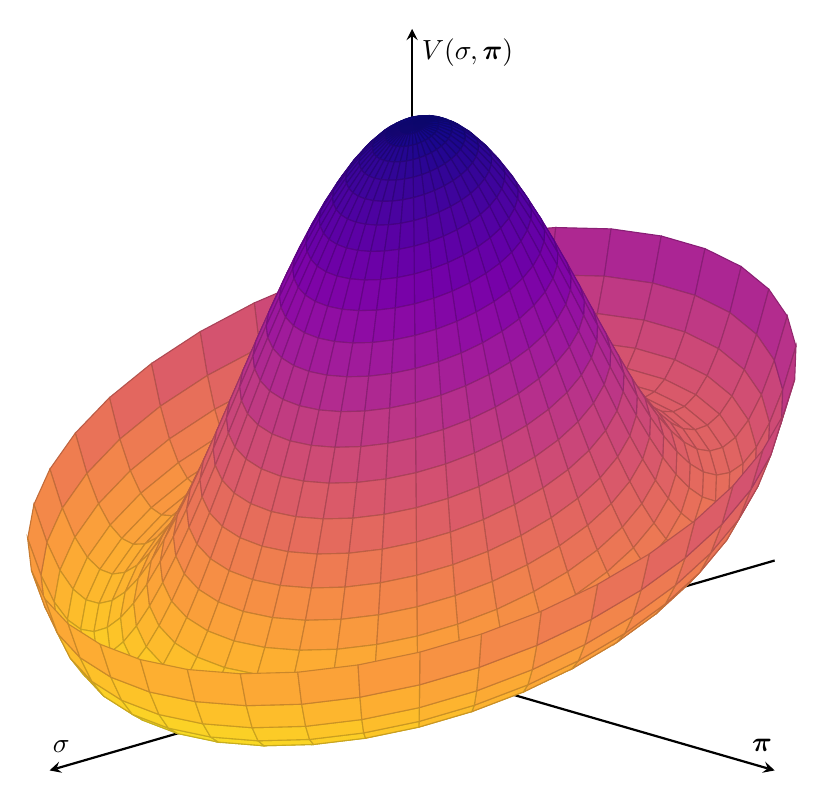
\begin{tikzpicture}
\begin{axis}[
	width = 20cm, height=15cm,
	%title = {Potential},
	xlabel = $\sigma$, ylabel = $\vec\pi$, zlabel = {$V(\sigma,\vec\pi)$},
	xmin=-4.0, xmax=+4.0, ymin=-4.0, ymax=+4.0, zmin=0, zmax=2.2,
	xtick=\empty, ytick=\empty, ztick=\empty,
	axis lines=center,
	axis line style = thick,
	view={135}{25},
	%colormap/blackwhite, mesh/interior colormap name=plasmarev,
]
	\addplot3 [surf, thin, domain=0:3.0, domain y=0:2*pi, samples=30, samples y=40, z buffer=sort] ({x*cos(deg(y))},{x*sin(deg(y))},{-1/2*((x*cos(deg(y)))^2+(x*sin(deg(y)))^2) + 1/24*((x*cos(deg(y)))^2+(x*sin(deg(y)))^2)^2 + 3/2 - 0.15*x*cos(deg(y)) + 0.15*sqrt(6)});
	%\addplot3 [domain=0:2*pi, samples=50, samples y=1] ({sqrt(6)*cos(deg(x))},{sqrt(6)*sin(deg(x))},{0});
\end{axis}
\end{tikzpicture}
\caption{\label{fig:lsm:potential}%
	A two-dimensional realization of the potential \eqref{eq:lsm:potential} looks like a Mexican hat, tilted along the $\sigma$-axis by the explicit symmetry breaking parameter $h$.
	If $h = 0$, the hat is upright with a continuous range of minima around $\sigma^2 + \vec\pi^2 = -6m^2 / \lambda$;
	while if $h \neq 0$, the hat is tilted and has a unique global minimum determined by equation \eqref{eq:lsm:ground_state_implicit}.
}
\end{figure}

\section{Lagrangian, symmetries and physical justification}
\label{sec:lsm:vacuum}

The Lagrangian density for the linear sigma model coupled to quarks is \cite{ref:lsm_2f}
\begin{equation}
	\lagr = \bar{q} \Big[ i \slashed\partial + \mu \gamma^0 - g \big( \sigma + i \gamma^5 \vec\tau \cdot \vec\pi \big) \Big] q
	      + \frac12 \Big[ \big( \partial_\mu \sigma \big) \big( \partial^\mu \sigma \big) + \big( \partial_\mu \vec\pi \big) \big( \partial^\mu \vec\pi \big) \Big] - \pot(\sigma,\vec\pi)
\label{eq:lsm:lagrangian}
\end{equation}
with the meson potential
\begin{equation}
	\pot(\sigma, \vec\pi) = \frac{m^2}{2} \big( \sigma^2 + \vec\pi^2 \big) + \frac{\lambda}{4!} \big( \sigma^2 + \vec\pi^2 \big)^2 - h \sigma .
\label{eq:lsm:potential}
\end{equation}
The quark fields behave as in the MIT bag model Lagrangian \eqref{eq:mit:lagrangian} with $N_f=2$ flavor indices $\{u,d\}$, $N_c=3$ color indices and four Dirac spinor indices, and are coupled to two quark chemical potentials with the flavor-space matrix $\mu = \diag (\mu_u, \mu_d)$.
However, they are now seemingly massless and coupled to a $\sigma$ meson and three pions $\vec\pi = [\pi^+, \pi^-, \pi^0]^T$ with a Yukawa coupling $g$ and the Pauli matrices \eqref{eq:tft:pauli_matrices}.
The meson potential features three couplings $m^2<0$, $\lambda>0$ and $h>0$.

Like quantum chromodynamics, the quark-meson model Lagrangian \eqref{eq:lsm:lagrangian} has a vector $U(1)_V$ and an axial $U(1)_A$ symmetry shown in \cref{sec:master_intro:qcd}.
In contrast to the mass-conditional chiral symmetry of quantum chromodynamics, however,
the Lagrangian \eqref{eq:lsm:lagrangian} is \emph{unconditionally} invariant under a $SU(2)_L \times SU(2)_R$ transformation when $h=0$ and $\mu = 0$.
To see this, first express the Yukawa coupling term with left-handed and right-handed chiral fields $q_\pm = P_\pm q$:
\begin{equation}
\begin{aligned}
	\bar{q} \big[\sigma + i \gamma^5 \vec{\tau} \cdot \vec{\pi}\big] q &= \bar{q} \big[ (P_+ + P_-) \sigma + (P_+ - P_-) i \vec{\tau} \cdot \vec{\pi}\big] q && \; \big( P_\pm = \tfrac{1}{2} (1 \pm \gamma^5) \big) \\
	                                                           %&= \bar{q} \big[ P_+ (\sigma + i \vec{\tau} \cdot \vec{\pi}) + P_- (\sigma - i \vec{\tau} \cdot \vec{\pi}) \big] q && \; \big( \text{distributivity} \big)\\
	                                                           &= \bar{q} \big[ P_+ \phi + P_- \phi^\dagger\big] q && \; \big( \text{define } \phi=\sigma+i\vec{\tau}\cdot\vec{\pi} \big) \\
	                                                           &= \bar{q} \big[ P_+^2 \phi + P_-^2 \phi^\dagger\big] q && \; \big( \text{$P_\pm=P_\pm^2$ lives in spinor-space} \big) \\
	                                                           &= \bar{q} \big[ P_+ \phi P_+ + P_- \phi^\dagger P_-\big] q && \; \big( \text{$\phi$ lives in flavor-space} \big)\\
	                                                           &= \bar{q}_- \phi \, q_+ + \bar{q}_+ \phi^\dagger q_- && \; \big( \text{$P_\pm q = q_\pm$, $\bar{q} P_\pm = (P_\mp q)^\dagger \gamma^0 = \bar{q}_\mp$} \big).\\
\end{aligned}
\label{eq:lsm:yukawa_symmetry}
\end{equation}
Second, note that the meson potential \eqref{eq:lsm:potential} with $h=0$ only depends on the flavor-space trace
\begin{equation}
	\tfrac12 \trace\big[\phi^\dagger \phi\big] = \tfrac12 \big( \underbrace{\trace\big[1\big]}_2 \sigma^2 - i^2 \underbrace{\trace\big[\tau_a \tau_b \big]}_{2 \delta_{ab}} \pi_a \pi_b \big) = \sigma^2 + \vec{\pi}^2.
\label{eq:lsm:meson_symmetry}
\end{equation}
Under the $SU(2)_L \times SU(2)_R$ transformation 
\begin{equation}
	q_+ \rightarrow U_+ q_+, \qquad
	q_- \rightarrow U_- q_-
	\qquad \text{and} \qquad
	\phi   \rightarrow U_- \phi U_+^\dagger,
\label{eq:lsm:symmetry_transformation}
\end{equation}
the Yukawa interaction \eqref{eq:lsm:yukawa_symmetry},
the meson potential argument \eqref{eq:lsm:meson_symmetry}
and hence the Lagrangian \eqref{eq:lsm:lagrangian} are invariant.
This proves the claimed unconditional $SU(2)_L \times SU(2)_R$ symmetry when $h=0$ and $\mu=0$.
Since the group $SU(2)_L \times SU(2)_R$ is isomorphic to $O(4)$,
the symmetry can equivalently be understood by considering the meson fields as a four-vector $[\sigma, \vec{\pi}]^T$
and noting that the meson potential \eqref{eq:lsm:potential} is invariant under rotation of this vector in four-space.

What can be the relevance of this unconditional symmetry,
when it was precisely the \emph{breaking} of it that led to the chiral symmetry breaking \eqref{eq:qcd:symmetry_breaking_pattern} of quantum chromodynamics in \cref{sec:master_intro:qcd}?
The short answer is that at the end of the day,
the different mathematical symmetries give rise to the \emph{same} physical consequences.
The longer answer follows below.

In the vacuum, the fermions do not contribute to the grand potential,
and the ground state values $\sigma = \avg{\sigma}$ and $\vec{\pi} = \avg{\vec{\pi}}$
are given by minima of the meson potential $\pot(\avg{\sigma},\avg{\vec{\pi}})$ illustrated in \cref{fig:lsm:potential}.
From its definition \eqref{eq:lsm:potential},
we see that they are given by
\begin{equation}
	%\vec{\pi} = \avg{\vec{\pi}}
	%\quad \text{and} \quad
	%\sigma = \avg{\sigma}
	%\pdv{\pot}{\sigma}_{(\sigma,\vec\pi)=(\avg{\sigma},\vec{0})} = m^2 \avg{\sigma} + \frac{\lambda}{6} \avg{\sigma}^3 - h = 0.
	\pdv{\pot}{\pi_a} = \avg{\pi_a} \Big[ m^2 + \frac{\lambda}{6} \big(\avg{\sigma}^2 + \avg{\vec{\pi}}^2\big) \Big] = 0
	\quad \text{and} \quad
	\pdv{\pot}{\sigma} = \avg{\sigma} \Big[ m^2 + \frac{\lambda}{6} \big(\avg{\sigma}^2 + \avg{\vec{\pi}}^2\big) \Big] - h = 0.
\label{eq:lsm:ground_state_implicit}
\end{equation}
The qualitative nature of the solutions depend on whether $h$ vanishes:
\begin{itemize}
\item In the \textbf{chiral limit} $h=0$,
      the ground state solutions are a degenerate range of minima along the circle $\avg{\sigma}^2+\avg{\vec{\pi}}^2=-6m^2/\lambda$,
      sometimes referred to as a vacuum manifold.
      Without any loss of generality, we pick the one at $\avg{\sigma} = \sqrt{-6m^2/\lambda}>0$ and $\avg{\vec{\pi}}=0$.
\item At the \textbf{physical point} $h \neq 0$,
      the ground state of the potential is a unique global minimum at $\avg{\sigma} \neq 0$ and $\avg{\vec{\pi}}=0$ determined implicitly by equation \eqref{eq:lsm:ground_state_implicit}.
\end{itemize}
Note that $\avg{\vec{\pi}} = 0$ in both cases.
To account for quantum fluctuations $\tilde{\sigma}$ and $\tilde{\vec{\pi}}$ of $\sigma$ and $\vec{\pi}$ around the ground states $\avg{\sigma}$ and $\avg{\vec{\pi}}$,
let us write
\begin{equation}
	\sigma = \avg{\sigma} + \tilde{\sigma}
	\qquad \text{and} \qquad
	\vec\pi = \avg{\vec\pi} + \tilde{\vec{\pi}}.
\end{equation}
Up to second order in the quantum fluctuations,
the Lagrangian \eqref{eq:lsm:lagrangian} becomes
\begin{equation}
	\lagr = \sum_{f=1}^{\smash{N_f}} \sum_{c=1}^{N_c} \bar{q} \Big[ i \slashed\partial + \mu \gamma^0 - m_q \Big] q
	      + \frac12 \Big[ \big( \partial_\mu \tilde{\sigma} \big) \big( \partial^\mu \tilde{\sigma} \big) + \big( \partial_\mu \tilde{\vec\pi} \big) \big( \partial^\mu \tilde{\vec\pi} \big) \Big] - \pot(\sigma,\vec\pi) , %\pot(\avg{\sigma}+\tilde{\sigma},\avg{\vec\pi}+\tilde{\vec\pi}) ,
\end{equation}
with the second-order meson potential \eqref{eq:lsm:potential}
\begin{equation}
	\pot(\sigma,\vec\pi) = \pot(\avg{\sigma},\avg{\vec\pi}) + h \tilde{\sigma} + \frac12 m_\sigma^2 \tilde{\sigma}^2 + \frac12 m_\pi^2 \tilde{\pi}^2,
\end{equation}
where the quark and meson fields have acquired the effective masses
\begin{subequations}
\begin{align}
	m_q &= g \avg{\sigma}, \label{eq:lsm:mass_quark} \\
	m_\sigma^2 &= \pdv[2]{\pot}{\sigma}\iffalse_{\substack{\sigma=\avg{\sigma}\\\vec{\pi}=\avg{\vec{\pi}}}}\fi    = m^2 + \frac{\lambda}{2} \avg{\sigma}^2 \equalexplabove{\smash[t]{\text{ by \eqref{eq:lsm:ground_state_implicit}}}} \frac{3h}{\avg{\sigma}} - 2 m^2 , \label{eq:lsm:mass_sigma} \\
	m_\pi^2    &= \pdv[2]{\pot}{\vec{\pi}}\iffalse_{\substack{\sigma=\avg{\sigma}\\\vec{\pi}=\avg{\vec{\pi}}}}\fi = m^2 + \frac{\lambda}{6} \avg{\sigma}^2 \equalexplbelow{\smash[b]{\text{ by \eqref{eq:lsm:ground_state_implicit}}}} \frac{h}{\avg{\sigma}} . \label{eq:lsm:mass_pi}
\end{align}%
\label{eq:lsm:mass_sigmapi}%
\end{subequations}%

Note that the up and down quarks have a degenerate mass $m_u = m_d = m_q$.
In nature, isospin symmetry is seemingly only slightly broken, and the up and down quark masses are indeed almost equal.
The (squared) meson masses $m_\sigma^2$ and $m_\pi^2$ are called (squared) \emph{curvature masses}
due to their relation with the second derivative of the potential.
They coincide with the physical pole masses of the particles' propagators
only at tree level, where loop effects are neglected.

The qualitative nature of the pions depends on whether $h$ vanishes:
\begin{itemize}
\item In the \textbf{chiral limit} $h = 0$ the $SU(2)_L \times SU(2)_R$ symmetry \eqref{eq:lsm:symmetry_transformation} is exact,
      and we saw above that there is a vacuum manifold of ground states.
      Upon committing to the minimum above with $\avg{\sigma} \neq 0$ and $\avg{\vec{\pi}} = 0$, the $O(4)$ rotation symmetry of the four original meson fields $[\sigma,\vec\pi]^T$ is spontaneously broken
      to rotation of only the three pion quantum fluctuations $\tilde{\vec\pi}$ in $O(3)$.
      Accordingly, the pion mass \eqref{eq:lsm:mass_pi} vanishes and the three pions are indeed Goldstone bosons associated with spontaneous symmetry breaking.
\item At the \textbf{physical point} $h \neq 0$, the $SU(2)_L \times SU(2)_R$ symmetry \eqref{eq:lsm:meson_symmetry} is explicitly broken,
      and we saw above that there is a unique ground state.
      Accordingly, the pions gain small masses \eqref{eq:lsm:mass_pi} and are pseudo-Goldstone bosons.
\end{itemize}
\label{elaborate on mexican hat analogy, brim, tip/tilt, etc.}
Unlike the resulting pions, the $\sigma$ particle is the \emph{cause} of the symmetry breaking,
and there is no reason for its mass \eqref{eq:lsm:mass_sigma} to vanish.
Speaking brutally to make a point, the $\sigma$ meson is only a mere means to an end to generate the chiral symmetry breaking and three pions,
which are our favorite spoiled children in this group of four meson siblings.

To summarize: although the linear sigma model symmetry breaking pattern
\begin{equation}
	SU(2) \times SU(2) \simeq O(4) \qquad \longrightarrow \qquad O(3)
\end{equation}
is \emph{different} from the quantum chromodynamics symmetry breaking pattern \eqref{eq:qcd:symmetry_breaking_pattern} ``under the hood'',
it gives rise to exactly the \emph{same} pion degrees of freedom ``on the outside''.
Practically speaking, the two different symmetry breaking patterns are therefore indistinguishable,
and according to Weinberg's philosophy presented in \cref{sec:master_intro:qcd}
the quark-meson model is an appropriate effective model of quantum chromodynamics at low energy.
The parameter $h \neq 0$ only serves to explicitly break the symmetry into an approximate one,
just like the quark masses explicitly break the chiral symmetry of quantum chromodynamics.
This is the physical justification of the quark-meson model.

\section{Grand potential}
\label{sec:lsm:grand_potential}

With our recently gained faith in the quark-meson model,
we set out to calculate its grand potential \eqref{eq:master_intro:grand_potential}.
With the quark fields $q$, the meson fields $\sigma$ and $\vec\pi$
and the coupling of conserved currents $j^\mu = \bar{q} \gamma^\mu q$ to chemical potentials $\mu$ already baked into the Lagrangian \eqref{eq:lsm:lagrangian},
the partition function \eqref{eq:master_intro:partition_function} is
\begin{equation}
	Z = \oint_- \pathintdif \bar{q} \oint_- \pathintdif q \oint_+ \pathintdif \sigma \oint_+ \pathintdif \vec\pi \exp \left\{ \int_0^\beta \dif \tau \int_V \dif^3 x \, \lagr_E[\bar{q}, q, \sigma, \vec\pi]  \right\} .
\end{equation}
To calculate it we will use the \textbf{mean-field approximation} for the bosonic fields,
replacing them by their \emph{yet unknown} expectation values $\avg{\sigma}$ and $\avg{\vec\pi}$ in the classical ground state
and simply ignoring their quantum fluctuations $\tilde{\sigma}$ and $\tilde{\vec\pi}$.
In contrast we will give the fermions full treatment,
motivated by their more dramatic behavior at zero temperature.
After calculating the grand potential with unknown mean fields,
their precise values are found \emph{self-consistently} with the original assumption of them being minima of the grand potential by solving
\begin{equation}
	\pdv{\Omega}{\avg{\sigma}} = \pdv{\Omega}{\avg{\vec\pi}} = 0.
\label{eq:lsm:gap_equation}
\end{equation}
We call this the \textbf{self-consistency equation} for the mean fields.
For example, the mean-field approximation is also famously used in the Bardeen-Cooper-Schrieffer theory of superconductivity to determine an energy gap.
There it is called the \textbf{gap equation}, 
and it can be useful to know that this name lives on as a relic in completely different applications, too.

In our treatment we will also neglect pion condensation and assume that $\avg{\vec\pi}=0$ \emph{always} vanishes,
so that only $\avg{\sigma}$ needs to be determined.
As shown by \cite{ref:jo_lsm_pion_condensation,ref:jo_lsm_consistent}, for example,
this is known to be true at $T=0$ when the isospin chemical potential \eqref{eq:master_intro:chemical_potentials_transformed} does not exceed half the pion mass.
This assumption is subject to a self-consistency check later.
In the bosonic mean-field approximation, the partition function of the Lagrangian \eqref{eq:lsm:lagrangian} reads
\begin{equation}
	Z = \oint_- \pathintdif \bar{q} \oint_- \pathintdif q \exp \bigg\{ \int_0^{\beta} \dif \tau \! \int_V \dif^3 x \Big[ \bar{q} \big( i \slashed\partial - m_q + \mu_f \gamma^0 \big) q - \pot(\avg{\sigma},\vec{0}) \Big] \bigg\}.
\end{equation}
The meson potential is independent of the fields and can be pulled out of the integrals,
while the fermionic contribution decouples into a product of identical integrals.
We therefore have
\begin{equation}
\begin{split}
	%\log Z &= -\frac12 \beta V m^2 \avg{\sigma}^2 - \frac{\lambda}{4!} \beta V \avg{\sigma}^4 + \beta V h \avg{\sigma} \\
	       %&+ \sum_{f=1}^{N_f} \sum_{c=1}^{N_c} \log \oint_- \pathintdif \bar{q}_f^c \oint_- \pathintdif q_f^c \exp \left\{ \int_0^\beta \dif \tau \int_V \dif^3 x \, \bar{q}_f^c (i \slashed\partial + \mu_f \gamma^0 - m_q) q_f^c \right\} .
	\log Z = -\pot(\avg{\sigma},\vec{0}) + \sum_{f=1}^{\smash{N_f}} \sum_{c=1}^{N_c} \log \oint_- \!\! \pathintdif \bar{q}_{f,c} \oint_- \!\! \pathintdif q_{f,c} \exp \bigg\{ \! \int_0^\beta \! \dif \tau \int_V \! \dif^3 x \, \bar{q}_{f,c} \big(i \slashed\partial + \mu_f \gamma^0 - m_q\big) q_{f,c} \! \bigg\} .
\end{split}
\end{equation}
We have already calculated the path integral in the last term
from equation \eqref{eq:tft:dirac_partition_function_first} to equation \eqref{eq:tft:dirac_partition_function}.
Here we get a factor $\sum_{c=1}^{N_c} = N_c$ from the color sum because the summand is independent of $c$,
while the flavor sum $\sum_{f=1}^{\smash{N_f}}$ yields $N_f$ terms that differ only by the chemical potential $\mu_f$ associated with each quark flavor. 
Thus, the grand potential \eqref{eq:master_intro:grand_potential} is
\begin{equation}
\begin{split}
	%\log Z &= -\frac12 \beta V m^2 \avg{\sigma}^2 - \frac{\lambda}{4!} \beta V \avg{\sigma}^4 + \beta V h \avg{\sigma} \\
	       %&+ 2 V N_c \sum_{f=1}^{N_f} \int \frac{\dif^3 p}{(2 \pi)^3} \left\{ \beta E(\vec{p}) + \log \left[ e^{-\beta (E(\vec{p}) - \mu_f)}+1 \right] + \log \left[ e^{-\beta (E(\vec{p}) + \mu_f)} + 1\right] \right\} ,
	\Omega = \pot(\avg{\sigma},\vec{0}) - \frac{2 N_c}{\beta} \sum_{f=1}^{\smash{N_f}} \int \frac{\dif^3 p}{(2 \pi)^3} \left\{ \beta E(\vec{p}) + \log \left[ e^{-\beta (E(\vec{p}) - \mu_f)}+1 \right] + \log \left[ e^{-\beta (E(\vec{p}) + \mu_f)} + 1\right] \right\} ,
\end{split}
\label{eq:lsm:potential_divergent_logz0}
\end{equation}
with the dispersion relation $E(\vec{p}) = \sqrt{\smash[b]{p^2 + m_q^2}}$.
We work in the zero-temperature approximation $T=0$ and choose positive chemical potentials,
so the anti-particle contribution from the last term in curly brackets vanishes.
The integral of the middle term in curly brackets was calculated in the zero-temperature pressure $P=-\Omega$ in equation \eqref{eq:nstars:pressure_zeroT}.
This time we also include and renormalize the infinite vacuum contribution from the integral of the first term in curly brackets.
It is called the \emph{Dirac sea}, and we renormalize it in the modified minimal subtraction scheme in \cref{chap:diracsea}.
Reinstating $x_f = p_f / m_q = \sqrt{\smash[b]{\mu_f^2-m_q^2}} / m_q$ into expression \eqref{eq:nstars:pressure_zeroT}
and including the renormalized Dirac sea \eqref{eq:diracsea:pole_expansion_modified},
the divergent grand potential \eqref{eq:lsm:potential_divergent_logz0} becomes
\begin{equation}
\begin{split}
	\Omega &= \pot(\avg{\sigma},\vec{0}) + N_c N_f \frac{m_q^4}{16 \pi^2} \Bigg[ \textcolor{red}{\frac{1}{\epsilon}} + \frac{3}{2} + \log\left(\frac{{\Lambda}^2}{m_q^2}\right) \Bigg] \\
	       &- \sum_{f=1}^{\smash{N_f}} \frac{N_c}{24 \pi^2} \left[ \left( 2 \mu_f^2 - 5 m_q^2 \right) \mu_f \sqrt{\mu_f^2 - m_q^2} + 3 m_q^4 \asinh \left( \sqrt{\frac{\mu_{\smash{f}}^2}{m_q^2}-1} \right) \right] .
\end{split}
\label{eq:lsm:grand_potential_nonrenormalized}
\end{equation}
The renormalization has introduced a renormalization scale $\Lambda$ that we will determine later.
It also exposes the Dirac sea vacuum divergence in the $\epsilon$-pole \textcolor{red}{$N_c N_f m_q^4 / 16 \pi^2 \epsilon$}.
Recalling that $m_q=g \avg{\sigma}$ and glancing back at the meson potential \eqref{eq:lsm:potential},
we also see that this divergence can be removed by the term \textcolor{blue}{$\lambda \avg{\sigma}^4 / 24$} in $\pot(\avg{\sigma},\vec{0})$
if the quartic coupling is shifted to
\begin{equation}
	\lambda \rightarrow \lambda + \textcolor{blue}{\delta\lambda}
	\qquad \text{with the counterterm} \qquad
	\textcolor{blue}{\delta\lambda = -N_c N_f \frac{3 g^4}{2 \pi^2 \epsilon}} .
\end{equation}
Then $\textcolor{red}{N_c N_f m_q^4 / 16 \pi^2 \epsilon} + \textcolor{blue}{\delta\lambda \avg{\sigma}^4 / 24} = 0$,
demonstrating that the theory is renormalizable.
Adding free electrons to the mix, the finite and renormalized grand potential is finally
\begin{equation}
\begin{split}
	\Omega(\avg{\sigma},\vec{\mu}) &= \pot(\avg{\sigma},\vec{0}) + N_c N_f \frac{m_q^4}{16 \pi^2} \Bigg[ \frac{3}{2} + \log\left(\frac{{\Lambda}^2}{m_q^2}\right) \Bigg] \\
	                               %&- \frac{N_c}{24 \pi^2} \sum_{f=\{u,d\}} \left[ \left( 2 \mu_f^2 - 5 m_q^2 \right) \mu_f \sqrt{\mu_f^2 - m_q^2} + 3 m_q^4 \asinh \left( \sqrt{\frac{\mu_{\smash{f}}^2}{m_q^2}-1} \right) \right] \\
	                               %&- \frac{  1}{24 \pi^2} \left[ \left( 2 \mu_e^2 - 5 m_e^2 \right) \mu_e \sqrt{\mu_e^2 - m_e^2} + 3 m_e^4 \asinh \left( \sqrt{\frac{\mu_e^2}{m_e^2}-1} \right) \right] .
	                               &-\sum_{f=1}^{\smash{N_f}} \frac{N_c}{24 \pi^2} \left[ \left( 2 \mu_f^2 - 5 m_q^2 \right) \mu_f \sqrt{\mu_f^2 - m_q^2} + 3 m_q^4 \asinh \left( \sqrt{\frac{\mu_{\smash{f}}^2}{m_q^2}-1} \right) \right] \\
	                               &-\phantom{\sum} \, \frac{1}{24 \pi^2} \left[ \left( 2 \mu_e^2 - 5 m_e^2 \right) \mu_e \sqrt{\mu_e^2 - m_e^2} \, + 3 m_e^4 \asinh \left( \sqrt{\frac{\mu_{\smash{e}}^2}{m_e^2}-1} \right) \right].
\end{split}
\label{eq:lsm:grand_potential}
\end{equation}
As in the MIT bag model,
the particle densities are
\begin{equation}
	n_f = -\pdv{\Omega}{\mu_f} = \frac{N_c}{3 \pi^2} \Big( \mu_f^2 - m_q^2 \Big)^{\frac32}
	\qquad \text{and} \qquad
	n_e = -\pdv{\Omega}{\mu_e} = \frac{  1}{3 \pi^2} \Big( \mu_e^2 - m_e^2 \Big)^{\frac32},
\label{eq:lsm:particle_densities}%
\end{equation}%
and the pressure \eqref{eq:master_intro:pressure} and energy density \eqref{eq:master_intro:energy_density} follow at $T=0$.

% equivalent remark is made in Folkestad/Andersen 2019 "Thermodynamics and phase diagram of Polykaov-loop extended chiral models"
% ("one-loop large-N_c limit")
It can be argued that treating bosons and fermions to zero and one loops is \emph{inconsistent}.
However, note that the fermionic contribution to the grand potential \eqref{eq:lsm:grand_potential} is of order $\bigo(N_c^1)$,
while any purely bosonic contribution would necessarily only be of order $\bigo(N_c^0)$.
Hence, we can also make a case for our approach being \emph{consistent} in the large-$N_c$ limit.
Strictly speaking, this only holds if the number of loops is simultaneously restricted to one;
with two loops, for example, the $\bigo(N_c^1)$ Feynman diagram due to the $\bar{q} \sigma q$ Yukawa interaction should also be included.
Although only $N_c = 3$ in nature,
the large-$N_c$ approximation is in fact a common and well-studied approximation scheme of quantum chromodynamics.
\cite{ref:large_Nc_review}.

\section{Parameter fitting at tree-level}
\label{sec:lsm:parameter_fit}

To determine the four paremeters $g$, $m^2$, $\lambda$ and $h$ in the Lagrangian \eqref{eq:lsm:lagrangian},
we use measured values of the ground state $\avg{\sigma}=f_\pi$ and curvature masses $m_\sigma$, $m_\pi$ and $m_q$ in vacuum.
Inverting equations \eqref{eq:lsm:ground_state_implicit} and \eqref{eq:lsm:mass_sigmapi}, we then find the parameters
\begin{equation}
	g       = \frac{m_q}{f_\pi}, \quad % &\qquad& \text{(by \eqref{eq:lsm:mass_quark})} , \\
	h       = m_\pi^2 f_\pi, \quad % &\qquad& \text{(by \eqref{eq:lsm:mass_pi})} , \\
	m^2     = \frac{3m_\pi^2 - m_\sigma^2}{2} \quad \text{and} \quad % &\qquad& \text{(by \eqref{eq:lsm:mass_sigma})} , \\
	\lambda = \frac{3 m_\sigma^2 - 3 m_\pi^2}{f_\pi^2} .    % &\qquad& \text{(by \eqref{eq:lsm:ground_state_implicit})} .
\label{eq:lsm:parameters}
\end{equation}
According to \cite{ref:pdg_review_2021}, in vacuum the mean field $\avg{\sigma} = f_\pi = \SI{93}{\mega\electronvolt}$ is the pion decay constant,
$m_\pi = \SI{138}{\mega\electronvolt}$ is the average mass of the three pions
and the up and down quarks have almost equal masses $m_u \approx m_d \approx \SI{300}{\mega\electronvolt}$.
All of these quantities have low uncertainty.


\begin{figure}
\centering
\tikzsetnextfilename{2-flavor-potential-vacuum}
\begin{tikzpicture}
\begin{axis}[
	width = 15cm, height = 7cm,
	xmin=-500, xmax=+500, xtick distance = 100, minor x tick num=9,
	ymin=-11, ymax=+6, ytick distance=5, minor y tick num=4,
	xlabel = {$m_q \, / \, \si{\mega\electronvolt}$ }, ylabel = {$\Omega \, / \, f_\pi^4$},
	legend style = {at={(0.5,1.03)}, anchor=south}, legend columns=4,
	cycle list/YlOrRd-6,
]
\pgfplotsset{cycle list shift=+2} % skip weakest line
\addplot+ [] table [x=Deltax, y=Omega] {../code/data/LSM2F/potential_vacuum_sigma500.dat}; \addlegendentry{$m_\sigma = \SI{500}{\mega\electronvolt}$};
%\addplot+ [] table [x=Deltax, y=Omega] {../code/data/LSM2F/potential_vacuum_sigma550.dat}; \addlegendentry{$m_\sigma = \SI{550}{\mega\electronvolt}$};
\addplot+ [] table [x=Deltax, y=Omega] {../code/data/LSM2F/potential_vacuum_sigma600.dat}; \addlegendentry{$m_\sigma = \SI{600}{\mega\electronvolt}$};
%\addplot+ [] table [x=Deltax, y=Omega] {../code/data/LSM2F/potential_vacuum_sigma650.dat}; \addlegendentry{$m_\sigma = \SI{650}{\mega\electronvolt}$};
\addplot+ [] table [x=Deltax, y=Omega] {../code/data/LSM2F/potential_vacuum_sigma700.dat}; \addlegendentry{$m_\sigma = \SI{700}{\mega\electronvolt}$};
%\addplot+ [] table [x=Deltax, y=Omega] {../code/data/LSM2F/potential_vacuum_sigma750.dat}; \addlegendentry{$m_\sigma = \SI{750}{\mega\electronvolt}$};
\addplot+ [] table [x=Deltax, y=Omega] {../code/data/LSM2F/potential_vacuum_sigma800.dat}; \addlegendentry{$m_\sigma = \SI{800}{\mega\electronvolt}$};
%\addplot+ [] table [x=Deltax, y=Omega] {../code/data/LSM2F/potential_vacuum_sigma850.dat}; \addlegendentry{$m_\sigma = \SI{850}{\mega\electronvolt}$};
\end{axis}
\end{tikzpicture}
\caption{\label{fig:lsm:potential_sigma_mass}
Two-flavor grand potential \eqref{eq:lsm:grand_potential} in vacuum with $\vec{\mu}=\vec{0}$ for different $m_\sigma$.}
\end{figure}

On the other hand, the mass $m_\sigma$ is very uncertain and hard to choose.
Even in 2002, according to the $\sigma$ meson status update \cite{ref:sigma_meson_status},
it was only known to lie in the huge uncertainty range $\SI{400}{\mega\electronvolt} \leq m_\sigma \leq \SI{1200}{\mega\electronvolt}$.
Today \cite{ref:pdg_review_2021} places it in the tighter range $\SI{400}{\mega\electronvolt} \leq m_\sigma \leq \SI{550}{\mega\electronvolt}$.
Ideally we would like to use a value within this range, but there are several problems.
First, the vacuum potential $\pot(\avg{\sigma},\vec{0})$ plotted in \cref{fig:lsm:potential_sigma_mass} does not have a minimum and is therefore useless for $m_\sigma \lesssim \SI{500}{\mega\electronvolt}$,
and the same happens with the three-flavor model in \cref{chap:lsm3f}.
We therefore operate with the three values $m_\sigma = \{600,700,800\} \, \si{\mega\electronvolt}$ in the two models.
The different values will illustrate qualitatively different behaviors of the chiral phase transition.
This is the best we can do and must be regarded as a shortcoming of our model.
Since the $\sigma$ particle was introduced in an ad-hoc manner and as a mere means to an end for the pions anyway,
we argue that it is the most legitimate candidate for discrimination
and that a discrepancy in this parameter is tolerable and that of least evil.

\Cref{tab:lsm2f:parameters} summarizes the chosen input values for $\avg{\sigma}$, $m_\pi$, $m_\sigma$ and $m_q$ in vacuum and the corresponding output parameters $m^2$, $\lambda$, $g$ and $h$.

Note that the renormalization procedure also introduced an unknown parameter $\Lambda$.
To determine it, we require that the minimum of the grand potential \eqref{eq:lsm:grand_potential} in vacuum with $\vec{\mu}=0$
remains at the minimum $\avg{\sigma} = f_\pi$ of the vacuum potential $\pot(\avg{\sigma},\vec{0})$.
Since $\pdv{\pot}/{\avg{\sigma}} = 0$ at $\avg{\sigma}=f_\pi$ already by assumption, we only need
\begin{equation}
	\pdv{\Omega}{\avg{\sigma}} =
	\pdv*{\Bigg[ N_c N_f \frac{m_q^4}{16 \pi^2} \bigg( \frac32 + \log \frac{\Lambda^2}{m_q^2} \bigg) \Bigg] }{\avg{\sigma}} = 0,
	\quad \text{yielding} \quad
	\Lambda = \frac{g f_\pi}{\sqrt{e}} = \SI{182.0}{\mega\electronvolt}.
\label{eq:lsm:potential_vacuum_minimum}
\end{equation}

\begin{table}[t]
\centering
\caption{\label{tab:lsm2f:parameters}%
The variables in the left table are used as input to determine the model parameters in the right table.
Experimental values are taken from \cite{ref:pdg_review_2021}.
Three different values are used for $m_\sigma$, generating three different values of both $\lambda$ and $m^2$.
}
\begin{tabular}{ l r r }
	\toprule
	Variable & Model                                   & Experimental       \\
	\midrule
	$\avg{\sigma}=f_\pi$ & $\textbf{\SI{93}{\mega\electronvolt}}$  & \SI{92}{}-\SI{93}{\mega\electronvolt} \\
	%\midrule
	$m_u=m_d$            & $\textbf{\SI{300}{\mega\electronvolt}}$ & \approx \, \SI{300}{\mega\electronvolt} \\
	%\midrule
	$m_\sigma$           & $\textbf{\{600,700,800\}\,\si{\mega\electronvolt}}$ & \SI{400}{}-\SI{550}{\mega\electronvolt}          \\
	$m_\pi$              & $\textbf{\SI{138}{\mega\electronvolt}}$ & \SI{138}{\mega\electronvolt}                     \\
	\bottomrule
\end{tabular}
\hfill
\begin{tabular}{ l r }
	\toprule
	Parameter   & Model                                 \\
	\midrule
	$g$         & $\SI{3.23}{}$                         \\
	$\lambda$   & $\{118,163,215\}$                        \\
	$m^2$       & $-(\{389,465,540\} \, \si{\mega\electronvolt})^2$ \\
	$h$         & $(\SI{121}{\mega\electronvolt})^3$  \\
	%$\Lambda$   & $\SI{182}{\mega\electronvolt}$ \\
	\bottomrule
\end{tabular}
\end{table}

Also note that we have treated bosons to tree level and fit parameters to their curvature masses \eqref{eq:lsm:mass_sigmapi},
but handled fermions to one loop. 
This is also inconsistent, as the physical pole masses would really receive radiative loop corrections in this case.
In \cref{sec:lsm2f:refinement} we will investigate the effects of fitting the parameters consistently at one loop level in the large-$N_c$-limit,
and we will see that this also resolves the large discrepancy in the parameter $m_\sigma$.
\TODO{in LARGE-$N_c$ limit AND one-loop}

\section{Equation of state}

Before finding the general charge neutral equation of state,
it is easier and instructive to solve the special problem with imposed zero isospin $\mu_I=0$, or $\mu_u=\mu_d=\mu$.
This will give us some intuition for the shape of the grand potential in the charge-neutral case.
The chemical equilibrium constraint \eqref{eq:lsm:chemical_equilibrium} then says $\mu_e=0$,
so electrons are absent and only the two first lines in the grand potential \eqref{eq:lsm:grand_potential} contribute.
It is now a function $\Omega(\avg{\sigma},\mu)$ of only two variables that is easy to visualize, as done in \cref{fig:lsm:grand-potential-noisospin}.
Although we defined $\Omega$ as a function of $\avg{\sigma}$, we will discuss the following results in terms of $m_q = g \avg{\sigma}$ instead,
as it is easier to compare to the chemical potentials $\mu_f$.
We see that:
\begin{itemize}
\item For $\mu < \SI{300}{\mega\electronvolt} = m_q(f_\pi)$ the grand potential is independent of $\mu$,
      and we are in vacuum where only the first line of the grand potential \eqref{eq:lsm:grand_potential} contributes.
      By construction, the minimum lies at $\avg{\sigma} = f_\pi = \SI{93}{\mega\electronvolt}$.
      The feature that a \emph{range} of chemical potentials characterizes the vacuum is sometimes called the \emph{Silver Blaze property}.
      Chiral symmetry is spontaneously broken in vacuum, as discussed in \cref{sec:lsm:vacuum}.
\item For $\SI{300}{\mega\electronvolt} \leq \mu \lesssim \SI{400}{\mega\electronvolt}$,
      the quarks in the second line of the grand potential \eqref{eq:lsm:grand_potential} begin to contribute as we leave the vacuum state during the chiral transition.
      For $m_\sigma = \SI{700}{\mega\electronvolt}$ the minimum jumps \emph{discontinuously}, corresponding to a \emph{first-order phase transition}.
      On the other hand, for $m_\sigma = \SI{800}{\mega\electronvolt}$ its value changes considerably and quickly but still \emph{continuously},
      and there is \emph{no phase transition} -- this behavior is referred to as a \emph{crossover}.
\item For $\mu \gtrsim \SI{400}{\mega\electronvolt}$ the minimum approaches the ultra-relativistic limit $\avg{\sigma} \rightarrow 0$ asymptotically,
      but never quite reaches it,
      as chiral symmetry is gradually restored.
\end{itemize}

\begin{figure}[t]
\centering
\tikzsetnextfilename{grand-potential-noisospin}
\begin{tikzpicture}
\begin{groupplot}[
	group style={group size={2 by 1}, vertical sep=2.0cm, horizontal sep=0.05cm},
	view={170}{25},
	width=0.55\textwidth, height=8cm,
	xlabel = {$m_q \, / \, \si{\mega\electronvolt}$},
	colormap/OrRd, point meta min=0, point meta max=600,
	3d box=complete,
	unbounded coords=jump, % skip at nan (i.e. the phase transition)
	extra tick style={grid=major, grid style={dashed}},
	title style={text width={5cm}},
	xlabel style={sloped}, 
	ylabel style={sloped, xshift=-0.5cm}, yticklabel style={anchor=east},
	zticklabels={,,},
	title style={sloped like x axis},
%
	zmin=-40, zmax=+10,
	xmin=-525, xmax=+525,
	restrict x to domain=-550:+550,
	restrict z to domain=-50:+30,
	xtick distance=150, %minor x tick num=1,
	ytick distance=100, %minor y tick num=3,
]
\nextgroupplot[
	ylabel = {$\mu \, / \, \si{\mega\electronvolt}$},
	%zlabel = {$\Omega(m_q, \mu) \, / \, (\SI{100}{\mega\electronvolt})^4$},
	zlabel = {$\Omega(m_q, \mu)$},
	title = {\subcaption{\label{fig:lsm:grand-potential-noisospin-sigma700}$m_\sigma=\SI{700}{\mega\electronvolt}$}},
];
\addplot3 [surf, very thin, mesh/ordering=x varies, point meta={abs(\thisrow{Delta})}] table [x=Delta, y=mu, z=Omega] {../code/data/LSM2F/potential_noisospin_sigma_700.dat};
\addplot3 [blue, x filter/.expression={\thisrow{Delta0} < 150 ? x : nan}] table [x=Delta0, y=mu0, z=Omega0]     {../code/data/LSM2F/potential_noisospin_sigma_700.dat}; % plot line of minima
\addplot3 [blue, x filter/.expression={\thisrow{Delta0} > 150 ? x : nan}] table [x=Delta0, y=mu0, z=Omega0]     {../code/data/LSM2F/potential_noisospin_sigma_700.dat}; % plot line of minima
\addplot3 [gray, x filter/.expression={\thisrow{Delta0} < 150 ? x : nan}] table [x=Delta0, y=mu0, z expr={-40}] {../code/data/LSM2F/potential_noisospin_sigma_700.dat}; % plot its "shadow" in bottom plane
\addplot3 [gray, x filter/.expression={\thisrow{Delta0} > 150 ? x : nan}] table [x=Delta0, y=mu0, z expr={-40}] {../code/data/LSM2F/potential_noisospin_sigma_700.dat}; % plot its "shadow" in bottom plane
\nextgroupplot[
	yticklabels={,,},
	zticklabels={,,},
	title = {\subcaption{\label{fig:lsm:grand-potential-noisospin-sigma800}$m_\sigma=\SI{800}{\mega\electronvolt}$}},
];
\addplot3 [surf, very thin, mesh/ordering=x varies, point meta={abs(\thisrow{Delta})}] table [x=Delta, y=mu, z=Omega] {../code/data/LSM2F/potential_noisospin_sigma_800.dat};
\addplot3 [blue] table [x=Delta0, y=mu0, z=Omega0]     {../code/data/LSM2F/potential_noisospin_sigma_800.dat}; % plot line of minima
\addplot3 [gray] table [x=Delta0, y=mu0, z expr={-40}] {../code/data/LSM2F/potential_noisospin_sigma_800.dat}; % plot its "shadow" in bottom plane
\end{groupplot}
\end{tikzpicture}
\caption{\label{fig:lsm:grand-potential-noisospin}%
	The grand potential \eqref{eq:lsm:grand_potential} with zero isospin, or $\mu_u = \mu_d = \mu$ and $\mu_e=0$, for $m_\sigma=\{700,800\} \, \si{\mega\electronvolt}$.
	The \textcolor{blue}{blue line} and its \textcolor{gray}{gray projection} show the minima $m_q = g \avg{\sigma}$ determined by the self-consistency equation \eqref{eq:lsm:gap_equation}.
}
\end{figure}

Our objective, however, is to determine the equation of state $\epsilon(P)$
when the chemical potentials are constrained by the conditions 
of $\beta$-equilibrium \eqref{eq:lsm:chemical_equilibrium}
and charge neutrality \eqref{eq:lsm:charge_neutrality}.
This means that we must not solve only the self-consistency equation \eqref{eq:lsm:gap_equation},
but the \emph{system} of equations
\begin{subequations}
\begin{align}
	0 &= \pdv{\Omega}{\avg{\sigma}} , \label{eq:lsm:minsys_min} \\
	%0 &= +\frac23 n_u - \frac13 n_d - n_e , \label{eq:lsm:minsys_charge} \\
	0 &= 2 \Big(\mu_u^2-m_q^2\Big)^\frac32 - \Big(\mu_d^2-m_q^2\Big)^\frac32 - \Big(\mu_e^2-m_e^2\Big)^\frac32 \label{eq:lsm:minsys_charge} \\
	\mu_d &= \mu_u + \mu_e .
\end{align}%
\label{eq:lsm:minsys}%
\end{subequations}%
This is a system of three equations for the four unknowns $\avg{\sigma}$, $\mu_u$, $\mu_d$ and $\mu_e$.
Remember that $m_q = g \avg{\sigma}$.
We parametrize solutions with one free variable, 
and calculate the densities \eqref{eq:lsm:particle_densities}, pressure \eqref{eq:master_intro:pressure}, energy density \eqref{eq:master_intro:energy_density}
and the equation of state $\epsilon(P)$ like in \cref{chap:mit}.

In particular, we now use $\avg{\sigma}$ as the free variable instead of $\mu$.
As revealed by peeking ahead at the results in \cref{fig:lsm:2-flavor-eos-parametrization},
the possible presence of a phase transition implies that
one $\mu$ can correspond to multiple $\avg{\sigma}$,
while all $\avg{\sigma}$ correspond to only one $\mu$ (outside vacuum).
It is therefore only the parametrization with $\avg{\sigma}$ that can capture the multiple solutions.

How should we normalize the pressure this time?
With the grand potential \eqref{eq:lsm:grand_potential},
the pressure $P = - \Omega$ will be nonzero in the vacuum because $\pot(f_\pi,\vec{0}) \neq 0$.
First, we therefore compute the pressure \emph{relative to} vacuum by shifting
\begin{equation}
	P \rightarrow P - P(\mu \leq \SI{300}{\mega\electronvolt}) = P + \pot(f_\pi,\vec{0}) .
\label{eq:lsm:pressure_bagless}
\end{equation}
Second, and like with the MIT bag model in \cref{chap:mit},
we allow for a bag constant $B$ by making the shift \eqref{eq:mit:bag_shift}.
After both shifts,
the pressure in vacuum is $P(\mu \leq \SI{300}{\mega\electronvolt}) = -B$
and the non-quark contribution to the general pressure is
\begin{equation}
	-B(\avg{\sigma}) = -\big[B+\pot(\avg{\sigma},\vec{0})-\pot(f_\pi,\vec{0})\big]
\label{eq:lsm:bag_pressure}
\end{equation}
from the first line of the grand potential \eqref{eq:lsm:grand_potential}.
Unlike the constant $B$ in the MIT bag model,
we can interpret $B(\avg{\sigma})$ as an dynamic bag pressure that ranges from $-B(f_\pi)=-B$ in vacuum to $-B(0) = -\big[B-\pot(f_\pi,\vec{0})\big]$ in the ultra-relativistic limit.
We will shortly come back to the minimum allowed bag constant, determined by solving the two-flavor inequality \eqref{eq:mit:bag_stability}.

\begin{figure}
\centering
\tikzsetnextfilename{2-flavor-eos}
\begin{tikzpicture}
\tikzset{declare function={
	muu(\muQ)=2/(1+2^(1/3))*\muQ;
	mud(\muQ)=2/(1+2^(-1/3))*\muQ;
	mue(\muQ)=2*(2^(1/3)-1)/(2^(1/3)+1)*\muQ;
	nq(\mu)=3/(3*pi^2)*(\mu)^3;
	ne(\mu)=1/(3*pi^2)*(\mu)^3;
	nconv=1.29619e-7;
}};
\begin{groupplot}[
	group style={group size={1 by 3}, vertical sep=1.9cm},
	width=13cm, height=7cm,
	extra tick style={grid=major, grid style={dashed}},
	minor tick num=9,
]
\nextgroupplot[
	xlabel={$\mu \, / \, \si{\mega\electronvolt}$},
	ylabel={$\{m_i,\mu_i\} \, / \, \si{\mega\electronvolt}$},
	%xmin=0, xmax=600, ymax=500, xtick distance=100, ytick distance=100, minor x tick num=9,
	xmin=0, xmax=700, xtick distance=100, minor x tick num=9,
	ymin=-20, ymax=700, ytick distance=100, 
	%ymax=600, 
	title={\subcaption{\label{fig:lsm:2-flavor-eos-parametrization}Parametrization of solutions}},
	legend cell align=left, legend pos=north west, reverse legend, legend columns=4, legend transposed,
];
\addplot+ [orange,    solid, very thick, opacity=0.4, forget plot, domain=0:700] {0};
\addplot+ [red,       solid, very thick, opacity=0.4, forget plot, domain=0:700] {muu(x)};
\addplot+ [darkgreen, solid, very thick, opacity=0.4, forget plot, domain=0:700] {mud(x)};
\addplot+ [blue,      solid, very thick, opacity=0.4, forget plot, domain=0:700] {mue(x)};
\addplot+ [black, very thick, opacity=0.4] {-100}; \addlegendentry{$m_{\phantom{\sigma}} = 0$};
\addplot+ [black, densely dotted] {-100}; \addlegendentry{$m_\sigma=\SI{600}{\mega\electronvolt}$};
\addplot+ [black, densely dashed] {-100}; \addlegendentry{$m_\sigma=\SI{700}{\mega\electronvolt}$};
\addplot+ [black, solid] {-100}; \addlegendentry{$m_\sigma=\SI{800}{\mega\electronvolt}$};
\addplot+ [blue,      densely dotted, opacity=0.7, forget plot] table [x expr={(\thisrow{muu}+\thisrow{mud})/2}, y=mue]    {../code/data/LSM2F/eos_sigma_600.dat};
\addplot+ [blue,      densely dashed, opacity=0.7, forget plot] table [x expr={(\thisrow{muu}+\thisrow{mud})/2}, y=mue]    {../code/data/LSM2F/eos_sigma_700.dat};
\addplot+ [blue,      solid, opacity=0.7] table [x expr={(\thisrow{muu}+\thisrow{mud})/2}, y=mue]    {../code/data/LSM2F/eos_sigma_800.dat}; \addlegendentry{$\mu_e$};
\addplot+ [darkgreen, densely dotted, opacity=0.7, forget plot] table [x expr={(\thisrow{muu}+\thisrow{mud})/2}, y=mud]    {../code/data/LSM2F/eos_sigma_600.dat};
\addplot+ [darkgreen, densely dashed, opacity=0.7, forget plot] table [x expr={(\thisrow{muu}+\thisrow{mud})/2}, y=mud]    {../code/data/LSM2F/eos_sigma_700.dat};
\addplot+ [darkgreen, solid, opacity=0.7] table [x expr={(\thisrow{muu}+\thisrow{mud})/2}, y=mud]    {../code/data/LSM2F/eos_sigma_800.dat}; \addlegendentry{$\mu_d$};
\addplot+ [red,       densely dotted, opacity=0.7, forget plot] table [x expr={(\thisrow{muu}+\thisrow{mud})/2}, y=muu]    {../code/data/LSM2F/eos_sigma_600.dat};
\addplot+ [red,       densely dashed, opacity=0.7, forget plot] table [x expr={(\thisrow{muu}+\thisrow{mud})/2}, y=muu]    {../code/data/LSM2F/eos_sigma_700.dat};
\addplot+ [red,       solid, opacity=0.7] table [x expr={(\thisrow{muu}+\thisrow{mud})/2}, y=muu]    {../code/data/LSM2F/eos_sigma_800.dat}; \addlegendentry{$\mu_u$};
\addplot+ [orange,    densely dotted, opacity=0.7, forget plot] table [x expr={(\thisrow{muu}+\thisrow{mud})/2}, y=mu] {../code/data/LSM2F/eos_sigma_600.dat};
\addplot+ [orange,    densely dashed, opacity=0.7, forget plot] table [x expr={(\thisrow{muu}+\thisrow{mud})/2}, y=mu] {../code/data/LSM2F/eos_sigma_700.dat};
\addplot+ [orange,    solid, opacity=0.7] table [x expr={(\thisrow{muu}+\thisrow{mud})/2}, y=mu] {../code/data/LSM2F/eos_sigma_800.dat}; \addlegendentry{$m_q$};
\addplot+ [black, every axis plot post/.append style={mark=*, mark options={fill=black}}, solid, domain=0:1, samples=2, forget plot] ({138/(1.12-0.88)}, {0.88*138/(1.12-0.88)+138*x}) node [pos=0.5, right] {$m_\pi$};


\nextgroupplot[
	xlabel={$\mu \, / \, \si{\mega\electronvolt}$}, ylabel={$n_i \, / \, (1/\si{\femto\meter\cubed})$},
	xmin=0, xmax=700, xtick distance=100, minor x tick num=9,
	ymin=-0.01, ymax=2.0, ytick distance=0.5, minor y tick num=4, restrict y to domain=-10:10,
	title={\subcaption{\label{fig:lsm:2-flavor-eos-density}Particle number densities}},
	legend cell align=left, legend pos=north west, reverse legend, legend columns=4, legend transposed,
];
\addplot+ [black, very thick, opacity=0.4] {-10}; \addlegendentry{$m_{\phantom{\sigma}} = 0$};
\addplot+ [black, densely dotted] {-10}; \addlegendentry{$m_\sigma=\SI{600}{\mega\electronvolt}$};
\addplot+ [black, densely dashed] {-10}; \addlegendentry{$m_\sigma=\SI{700}{\mega\electronvolt}$};
\addplot+ [black, solid] {-10}; \addlegendentry{$m_\sigma=\SI{800}{\mega\electronvolt}$};
\addplot+ [black, solid] {-10}; \addlegendentry{}; \addlegendimage{empty legend};
\addplot+ [red,       solid, very thick, opacity=0.4, forget plot, domain=0:700] {nq(muu(x))*nconv};
\addplot+ [darkgreen, solid, very thick, opacity=0.4, forget plot, domain=0:700] {nq(mud(x))*nconv};
\addplot+ [blue,      solid, very thick, opacity=0.4, forget plot, domain=0:700] {ne(mue(x))*nconv};
\addplot+ [blue,      densely dotted, opacity=0.7, forget plot] table [x expr={(\thisrow{muu}+\thisrow{mud})/2}, y=ne] {../code/data/LSM2F/eos_sigma_600.dat};
\addplot+ [blue,      densely dashed, opacity=0.7, forget plot] table [x expr={(\thisrow{muu}+\thisrow{mud})/2}, y=ne] {../code/data/LSM2F/eos_sigma_700.dat};
\addplot+ [blue,      solid, opacity=0.7] table [x expr={(\thisrow{muu}+\thisrow{mud})/2}, y=ne] {../code/data/LSM2F/eos_sigma_800.dat}; \addlegendentry{$n_e\,\,$};
\addplot+ [darkgreen, densely dotted, opacity=0.7, forget plot] table [x expr={(\thisrow{muu}+\thisrow{mud})/2}, y=nd] {../code/data/LSM2F/eos_sigma_600.dat};
\addplot+ [darkgreen, densely dashed, opacity=0.7, forget plot] table [x expr={(\thisrow{muu}+\thisrow{mud})/2}, y=nd] {../code/data/LSM2F/eos_sigma_700.dat};
\addplot+ [darkgreen, solid, opacity=0.7] table [x expr={(\thisrow{muu}+\thisrow{mud})/2}, y=nd] {../code/data/LSM2F/eos_sigma_800.dat}; \addlegendentry{$n_d\,\,$};
\addplot+ [red,       densely dotted, opacity=0.7, forget plot] table [x expr={(\thisrow{muu}+\thisrow{mud})/2}, y=nu] {../code/data/LSM2F/eos_sigma_600.dat};
\addplot+ [red,       densely dashed, opacity=0.7, forget plot] table [x expr={(\thisrow{muu}+\thisrow{mud})/2}, y=nu] {../code/data/LSM2F/eos_sigma_700.dat};
\addplot+ [red,       solid, opacity=0.7] table [x expr={(\thisrow{muu}+\thisrow{mud})/2}, y=nu] {../code/data/LSM2F/eos_sigma_800.dat}; \addlegendentry{$n_u\,\,$};

\nextgroupplot[
	xlabel={$P        \, / \, (\si{\giga\electronvolt\per\femto\meter\cubed})$},
	ylabel={$\epsilon \, / \, (\si{\giga\electronvolt\per\femto\meter\cubed})$},
	xmin=-0.005, xmax=0.05, ymin=0, ymax=0.7, xtick distance=0.01, ytick distance=0.1, minor y tick num=9, restrict y to domain=-1:+1,
	title={\subcaption{\label{fig:lsm:2-flavor-eos-eos}Equation of state}},
	legend cell align=left, legend pos=north west, legend transposed, legend columns=4,
];
\addplot+ [black, solid, opacity=0.7] table [x=Porg,y=epsilonorg] {../code/data/LSM2F/eos_sigma_800.dat}; \addlegendentry{$m_\sigma=\SI{800}{\mega\electronvolt}$}
%\addplot+ [black, solid, opacity=0.7, forget plot] table [x=P,y=epsilon] {../code/data/LSM2F/eos_sigma_800.dat};
\addplot+ [gray, densely dashed, opacity=0.7, forget plot] table [x=Porg,y=epsilonorg] {../code/data/LSM2F/eos_sigma_700.dat};
\addplot+ [black, densely dashed, opacity=0.7] table [x=P,y=epsilon] {../code/data/LSM2F/eos_sigma_700.dat}; \addlegendentry{$m_\sigma=\SI{700}{\mega\electronvolt}$}
\addplot+ [gray, densely dotted, opacity=0.7, forget plot] table [x=Porg,y=epsilonorg] {../code/data/LSM2F/eos_sigma_600.dat};
\addplot+ [black, densely dotted, opacity=0.7] table [x=P,y=epsilon] {../code/data/LSM2F/eos_sigma_600.dat}; \addlegendentry{$m_\sigma=\SI{600}{\mega\electronvolt}$}
\addplot+ [black, solid, very thick, opacity=0.4, domain=0:0.1] {3*x}; \addlegendentry{$m_{\phantom{\sigma}} = 0$};
\addplot+ [gray, solid, domain=0:0.01] {-0.01}; \addlegendentry{uncorrected}
\addplot+ [black, solid, domain=0:0.01] {-0.01}; \addlegendentry{\phantom{un}corrected}
\addlegendimage{empty legend}\addlegendentry{} % ski
\end{groupplot}
\end{tikzpicture}
\caption{\label{fig:lsm:2-flavor-eos}%
Properties of electrically charge neutral quark matter in $\beta$-equilibrium parametrized by the quark chemical potential $\mu = (\mu_u+\mu_d)/2$ in the two-flavor quark-meson model.
Upper panel \subref{fig:lsm:2-flavor-eos-parametrization} shows solutions to equation \eqref{eq:lsm:minsys},
middle panel \subref{fig:lsm:2-flavor-eos-density} the corresponding particle number densities \eqref{eq:lsm:particle_densities} and
lower panel \subref{fig:lsm:2-flavor-eos-eos} the corresponding equation of state $\epsilon(P)$ \textbf{\textcolor{gray}{before}} and \textbf{after} the Maxwell construction.
Three different values of $m_\sigma$ are used,
and the thickest lines show the massless solutions \eqref{eq:mit:densities_massless}, \eqref{eq:mit:eos_ur} and \eqref{eq:mit:chemical_potentials_massless_2f}.
}
\end{figure}

The detailed numerical implementation can be found in \cref{sec:num:qstars2f}.
We find the equation of state shown in \cref{fig:lsm:2-flavor-eos}:
\begin{itemize}
\item The phase transition or crossover behaves similarly as in \cref{fig:lsm:grand-potential-noisospin}:
      the grand potential \eqref{eq:lsm:grand_potential} and its minimum $\avg{\sigma}=m_q/g$ is independent of $\mu$ in vacuum where $\mu < \SI{300}{\mega\electronvolt}$;
      undergoes a crossover (with $m_\sigma \geq \SI{800}{\mega\electronvolt}$) or a first-order phase transition (with $m_\sigma < \SI{800}{\mega\electronvolt}$) for $\SI{300}{\mega\electronvolt} < \mu \lesssim \SI{400}{\mega\electronvolt}$;
      and approaches the ultra-relativistic limit $\avg{\sigma}\rightarrow 0$ for $\mu \gtrsim \SI{400}{\mega\electronvolt}$.
\item The isospin chemical potential $\mu_I=(\mu_u-\mu_d)/2$ increases with no bound as $\mu_u$ and $\mu_d$ grow apart,
      and its magnitude exceeds the half pion mass $m_\pi/2 = \SI{69}{\mega\electronvolt}$ at $\mu = \SI{575}{\mega\electronvolt}$.
      \emph{This means that our assumption of neglecting pion condensation is inconsistent!}
      A more detailed study should therefore take it into account, but this is outside our scope.
\item With $m_\sigma < \SI{800}{\mega\electronvolt}$ and the resulting phase transition,
      the parametrized $P$-$\epsilon$-curve corresponds to an \emph{ambiguous equation of state}.
      For very low pressures, one pressure corresponds to multiple energy densities.
      In this case we use the Maxwell construction described in \cite[equation 4.69]{ref:master_francesco} to produce an invertible and hence usable equation of state.
      With $m_\sigma \geq \SI{800}{\mega\electronvolt}$ and the crossover we do not need to think about this.
\item The ultra-relativistic solution obtained in \cref{sec:mit:eos} is restored as $\avg{\sigma} \rightarrow 0$.
      In particular, the slopes $\odv{\epsilon}/{P} = 3$ of the equations of state agree.
      Their relative offset is accounted for by making the bag shift \eqref{eq:mit:bag_shift}.
\item The equation of state always satisfies the microscopic stability criteria \eqref{eq:nstars:stability_speed_of_sound} and \eqref{eq:nstars:stability_pressure_energy_density}.
\item Although the electrons have an appreciable chemical potential $\mu_e$, their \emph{density} $n_e$ is hardly noticeable compared to the quark densities $n_u$ and $n_d$.
      Just like in \cref{chap:mit} the density is nonzero, only several orders of magnitude below the quark densities.
      Their main job is to ensure charge neutrality is met.
\end{itemize}

Moreover, the program in \cref{sec:num:qstars2f} solves the two-flavor inequality \eqref{eq:mit:bag_stability} numerically
and reports the lower bag bounds
\begin{subequations}
\begin{align}
	B \geq (\SI{110.6}{\mega\electronvolt})^4           \quad \Big(\text{or } B-\pot(f_\pi,\vec{0}) \geq (\SI{145.4}{\mega\electronvolt})^4\Big) \qquad \Big(m_\sigma = \SI{600}{\mega\electronvolt}\Big), \label{eq:lsm:bag_lower_bound_600} \\
	B \geq \phantom{0}(\SI{67.7}{\mega\electronvolt})^4 \quad \Big(\text{or } B-\pot(f_\pi,\vec{0}) \geq (\SI{146.3}{\mega\electronvolt})^4\Big) \qquad \Big(m_\sigma = \SI{700}{\mega\electronvolt}\Big), \label{eq:lsm:bag_lower_bound_700} \\
	B \geq \phantom{0}(\SI{27.0}{\mega\electronvolt})^4 \quad \Big(\text{or } B-\pot(f_\pi,\vec{0}) \geq (\SI{156.5}{\mega\electronvolt})^4\Big) \qquad \Big(m_\sigma = \SI{800}{\mega\electronvolt}\Big). \label{eq:lsm:bag_lower_bound_800}
\end{align}%%
\label{eq:lsm:bag_lower_bound}%
\end{subequations}%%
In the next chapter we study the three-flavor generalization of this model
and find the complementing upper bounds \eqref{eq:lsm3f:bag_upper_bound}
due to the strange matter hypothesis.
Note that these upper bounds almost coincide with the lower bounds,
so the inequalities can be squeezed into equalities \emph{if} the strange matter hypothesis is true.
The \emph{lower} bounds, on the other hand, are based on instability of two-flavor quark matter compared to hadronic matter and are trustworthy.
We focus our attention on the bag constants that lie \emph{at} the lower bounds \eqref{eq:lsm:bag_lower_bound},
as we saw in \cref{fig:mit:eos} that they generate stiffer equations of state and hence greater maximum masses,
and greater bag constants would be forbidden anyway \emph{if} the strange matter hypothesis holds.

As pointed out by \cite[section IV-B]{ref:quark_star_review}, it is generally meaningless to compare bag constants across models.
Anyway, note that because of the vacuum normalization \eqref{eq:lsm:pressure_bagless}, it is the bounds of $B-\pot(f_\pi,\vec{0})$, not $B$, that are comparable to the MIT bag model lower bound \eqref{eq:mit:bag_window}.

\section{Stellar solutions}

\begin{figure}[p]
\centering
\tikzsetnextfilename{2-flavor-mass-radius}
\begin{tikzpicture}
\begin{groupplot}[
	group style={group size={3 by 1}, vertical sep=0cm, horizontal sep=0.3cm},
	width=6cm, height=6cm,
	xmin=5, xmax=20, ymin=0.5, ymax=2.5, xtick distance=5, ytick distance=0.5, minor tick num=4, grid=major,
	point meta=explicit, point meta min=33, point meta max=36,
	%colorbar horizontal, colormap name=plasmarev, colorbar style={xlabel=$\log_{10} (P_c \, / \, \si{\pascal})$, xtick distance=1, minor x tick num=9, at={(0.5,1.03)}, anchor=south, xticklabel pos=upper},
	/tikz/declare function={
		e0 = 4.266500881855304e+37;
	},
]
\tikzset{
	Bpin/.style={gray, sloped, allow upside down=true, rotate=180, yshift=+0.4cm, font=\small},
}
\nextgroupplot[
	xlabel={$R \, / \, \si{\kilo\meter}$},
	ylabel={$M \, / \, M_\odot$}, %title={Mass-radius diagram for 2-flavor quark stars }, title style={yshift=2.0cm},
	title = {\subcaption{\label{fig:lsm:2-flavor-mass-radius-600}$m_\sigma = \SI{600}{\mega\electronvolt }$} $B^\frac14 = \{111,131,151\} \, \si{\mega\electronvolt}$},
];
\addplot+ [solid, mesh] table [x=R, y=M, meta expr={log10(\thisrow{P}*e0)}] {../code/data/LSM2F/stars_sigma_600_B14_111.dat}; % node [Bpin, pos=0.920] {$B = (\SI{27}{\mega\electronvolt})^4$};
\addplot+ [solid, mesh] table [x=R, y=M, meta expr={log10(\thisrow{P}*e0)}] {../code/data/LSM2F/stars_sigma_600_B14_131.dat}; % node [Bpin, pos=0.920] {$B = (\SI{27}{\mega\electronvolt})^4$};
\addplot+ [solid, mesh] table [x=R, y=M, meta expr={log10(\thisrow{P}*e0)}] {../code/data/LSM2F/stars_sigma_600_B14_151.dat}; % node [Bpin, pos=0.920] {$B = (\SI{27}{\mega\electronvolt})^4$};

\nextgroupplot[
	xlabel={$R \, / \, \si{\kilo\meter}$},
	yticklabels={,,},
	title = {\subcaption{\label{fig:lsm:2-flavor-mass-radius-700}$m_\sigma = \SI{700}{\mega\electronvolt}$} $B^\frac14 = \{68,88,108\} \, \si{\mega\electronvolt}$},
	colorbar horizontal, colormap name=plasmarev, colorbar style={width=11cm, ylabel=$\log_{10} (P_c \, / \, \si{\pascal})$, ylabel style={rotate=-90}, xtick distance=1, minor x tick num=9, at={(0.5,-0.3)}, anchor=north, xticklabel pos=lower},
];
\addplot+ [solid, mesh] table [x=R, y=M, meta expr={log10(\thisrow{P}*e0)}] {../code/data/LSM2F/stars_sigma_700_B14_68.dat};  % node [Bpin, pos=0.920] {$B = (\SI{27}{\mega\electronvolt})^4$};
\addplot+ [solid, mesh] table [x=R, y=M, meta expr={log10(\thisrow{P}*e0)}] {../code/data/LSM2F/stars_sigma_700_B14_88.dat};  % node [Bpin, pos=0.920] {$B = (\SI{27}{\mega\electronvolt})^4$};
\addplot+ [solid, mesh] table [x=R, y=M, meta expr={log10(\thisrow{P}*e0)}] {../code/data/LSM2F/stars_sigma_700_B14_108.dat}; % node [Bpin, pos=0.920] {$B = (\SI{27}{\mega\electronvolt})^4$};

\nextgroupplot[
	xlabel={$R \, / \, \si{\kilo\meter}$},
	yticklabels={,,},
	title = {\subcaption{\label{fig:lsm:2-flavor-mass-radius-800}$m_\sigma = \SI{800}{\mega\electronvolt}$} $B^\frac14 = \{27,47,67\} \, \si{\mega\electronvolt}$},
];
\addplot+ [solid, mesh] table [x=R, y=M, meta expr={log10(\thisrow{P}*e0)}] {../code/data/LSM2F/stars_sigma_800_B14_27.dat}; % node [Bpin, pos=0.920] {$B = (\SI{27}{\mega\electronvolt})^4$};
\addplot+ [solid, mesh] table [x=R, y=M, meta expr={log10(\thisrow{P}*e0)}] {../code/data/LSM2F/stars_sigma_800_B14_47.dat}; % node [Bpin, pos=0.920] {$B = (\SI{27}{\mega\electronvolt})^4$};
\addplot+ [solid, mesh] table [x=R, y=M, meta expr={log10(\thisrow{P}*e0)}] {../code/data/LSM2F/stars_sigma_800_B14_67.dat}; % node [Bpin, pos=0.920] {$B = (\SI{27}{\mega\electronvolt})^4$};
\node[scale=0.75] at (11.269, 1.775) {\goldenstar};

\end{groupplot}
\node [anchor=south, yshift=+1.5cm] at (group c2r1.north) {Two-flavor quark-meson model quark stars};
\end{tikzpicture}
\caption{\label{fig:lsm:2-flavor-mass-radius}%
	Mass-radius solutions of the Tolman-Oppenheimer-Volkoff equations \eqref{eq:master_intro:tov} parametrized by the central pressure $P_c$,
	using the equations of state for two-flavor quark matter in \cref{fig:lsm:2-flavor-eos-eos} modified by bag constants above the bounds \eqref{eq:lsm:bag_lower_bound}.
}

\bigskip

\tikzsetnextfilename{2-flavor-extreme-star}
\begin{tikzpicture}
\begin{groupplot}[
	group style={group size={2 by 2}, horizontal sep=1.2cm, vertical sep=0.4cm},
	width=8cm, height=6cm,
	ylabel style={yshift=-0.2cm},
	enlargelimits=false, xtick distance=1.0, minor xtick={0,0.1,...,11.3},
	legend cell align=left,
]
\nextgroupplot[
	xticklabels={,,},
	ymax=1.5, ytick distance=0.5, minor y tick num=4,
	ylabel={$\{\epsilon,P\} \, / \, (\si{\giga\electronvolt\per\femto\meter\cubed})$},
];
\addplot+ [blue] table [x=r, y=epsilon] {../code/data/LSM2F/star_sigma_800_B14_27_Pc_0.0012501.dat}; \addlegendentry{$\epsilon$};
\addplot+ [red] table [x=r, y=P] {../code/data/LSM2F/star_sigma_800_B14_27_Pc_0.0012501.dat}; \addlegendentry{$P$};
\nextgroupplot[
	ylabel=$m \, / \, M_\odot$,
	xticklabels={,,},
	ymax=2, ytick distance=0.5, minor y tick num=4,
];
\addplot+ [black] table [x=r, y=m] {../code/data/LSM2F/star_sigma_800_B14_27_Pc_0.0012501.dat};
\nextgroupplot[
	xlabel=$r \, / \, \si{\kilo\meter}$,
	ylabel=$\mu \, / \, \si{\mega\electronvolt}$,
	ymin=300, ymax=500, ytick distance=50, minor y tick num=4,
];
\addplot+ [black] table [x=r, y=muQ] {../code/data/LSM2F/star_sigma_800_B14_27_Pc_0.0012501.dat};
\nextgroupplot[
	xlabel=$r \, / \, \si{\kilo\meter}$,
	ylabel=$n_i \, / \, n_\text{sat}$,
	ymax=15, ytick distance=5, minor y tick num=4,
];
\addplot+ [red] table [x=r, y=nu] {../code/data/LSM2F/star_sigma_800_B14_27_Pc_0.0012501.dat}; \addlegendentry{$n_u$};
\addplot+ [darkgreen] table [x=r, y=nd] {../code/data/LSM2F/star_sigma_800_B14_27_Pc_0.0012501.dat}; \addlegendentry{$n_d$};
\addplot+ [blue] table [x=r, y=ne] {../code/data/LSM2F/star_sigma_800_B14_27_Pc_0.0012501.dat}; \addlegendentry{$n_e$};
\addplot+ [black, dashed, forget plot] table [x=r, y expr={(\thisrow{nu}+\thisrow{nd}+\thisrow{ns})/3}] {../code/data/LSM2F/star_sigma_800_B14_27_Pc_0.0012501.dat};
% cheat legend
\addplot+ [draw=none, black, solid] table [x=r, y expr={(\thisrow{nu}+\thisrow{nd}+\thisrow{ns})/3}] {../code/data/LSM2F/star_sigma_800_B14_27_Pc_0.0012501.dat}; \addlegendentry{$n_B$};
\end{groupplot}
\node (title) at ($(group c1r1.north)!0.5!(group c2r1.north)$) [above, yshift=\pgfkeysvalueof{/pgfplots/every axis title shift}]
{\goldenstar Maximum mass star ($m_\sigma=\SI{800}{\mega\electronvolt}$, $B^\frac14 = \SI{27}{\mega\electronvolt}$, $P_c=10^{34.727} \, \si{\pascal}$) };
\end{tikzpicture}
\caption{\label{fig:lsm:2-flavor-star}%
	Radial profiles for the
	pressure $P$,
	energy density $\epsilon$,
	cumulative mass $m$,
	quark chemical potential $\mu$,
	particle densities $n_i$
	and baryon density $n_B = (n_u+n_d)/3$
	for the maximum mass two-flavor quark star \goldenstar in \cref{fig:lsm:2-flavor-mass-radius}.
}
\end{figure}

With the equation of state, we now solve the Tolman-Oppenheimer-Volkoff equations \eqref{eq:master_intro:tov} with multiple bag pressures above the lower bounds \eqref{eq:lsm:bag_lower_bound}.
We find the mass-radius relations in \cref{fig:lsm:2-flavor-mass-radius}:
\begin{itemize}
\item For bag constants that just satisfy the lower bound \eqref{eq:lsm:bag_lower_bound},
      stars have maximum masses $1.7 \, M_\odot \leq M \leq 2.0 \, M_\odot$ and corresponding radii $R \approx \SI{11}{\kilo\meter}$
      depending on the value chosen for $m_\sigma$.
      The heaviest star has an average mass density of $\rho = M / (4 \pi R^3/3) = \SI{7e14}{\kilo\gram\per\liter}$!
\item For greater bag constants,
      the strange matter hypothesis is violated and both masses and radii decrease.
      With a sufficiently high $B$ one can cover any mass and radii below the greatest ones,
      and we therefore pay special attention to the lowest instability-respecting bag constants.
\item As $m_\sigma$ increases,
      the maximum mass decreases and becomes more resilient to changes in $B$, and stars tend to inflate up to larger sizes for low pressures.
      It therefore seems important to press $m_\sigma$ as close as possible 
      to its measured values $\SI{400}{\mega\electronvolt} \leq m_\sigma \leq \SI{550}{\mega\electronvolt}$
      in order to produce more massive stars.
\item The results are generally comparable to the MIT bag model solutions in \cref{fig:mit:mass_radius}.
\end{itemize}

Let us also examine the radial profiles of interesting quantities in a star.
The solution of the Tolman-Oppenheimer-Volkoff equations \eqref{eq:master_intro:tov} yields $P(r)$ and $m(r)$ directly,
and $\epsilon(r)$ is then easily computed from the equation of state $\epsilon(P)$.
Meanwhile, $\mu(r)$ can be obtained from $P(r)$ after inverting $P(\mu)$ to $\mu(P)$,
and $n_i(r)$ and other properties can then be looked up in \cref{fig:lsm:2-flavor-eos}.
In \cref{fig:lsm:2-flavor-star} we take an in-depth look at the maximum mass star without a phase transition:
\begin{itemize}
\label{list:lsm:2-flavor-star-discussion}
\item By definition, the pressure $P(R)=0$ vanishes at the surface $R=\SI{11.3}{\kilo\meter}$,
      and the corresponding cumulative mass $m(R)=M=\SI{1.77}{}\,M_\odot$ evaluates to the total mass.
\item The quark chemical potential $\mu(R)$ at the surface exceeds the vacuum value $\SI{300}{\mega\electronvolt}$ because of the bag shift \eqref{eq:mit:bag_shift}.
      Fortunately, the central value $\mu(0) = \SI{490}{\mega\electronvolt}$ does not exceed $\SI{575}{\mega\electronvolt}$,
      beyond which neglecting pion condensation was inconsistent. % in \cref{fig:lsm:2-flavor-eos-parametrization}.
\item The kink around $\mu \approx \SI{320}{\mega\electronvolt}$ corresponds to the chiral crossover and takes place very close to the surface of the star,
      and the star has a thin crust in which the particle densities rapidly drops to near-vanishing values and the cumulative mass flattens out.
%\item Hybrid neutron stars are typically assumed to consist of nuclear matter for $n_B \lesssim 2 n_\text{sat}$,
      %quark matter for $4 n_\text{sat} \lesssim n_B \lesssim 7 n_\text{sat}$ and something in-between for $2 n_\text{sat} \lesssim n_B \lesssim 4 n_\text{sat}$.
      %If the core of this quark star were to model the core of such a hybrid star,
      %it would have a radius $R' \approx \SI{5}{\kilo\meter}$, mass $M'=m(R')=\SI{0.45}{\kilo\meter}$ and central pressure $P_c \approx \SI{0.33}{\giga\electronvolt\per\femto\meter\cubed}$
      %and consist predominantly of quarks with twice as many up quarks as down quarks.
\end{itemize}

\iffalse
\TODO{just drop this part?
Having described we \emph{do} and \emph{should do}, let us also remark on what we \emph{did} and \emph{shouldn't do}.
A tempting and similar approach to minimizing $\Omega$ with respect to $\avg{\sigma}$ is to rather construct the potential $\Omega'(\avg{\sigma}, \mu_u) = \Omega(\avg{\sigma}, \mu_u, \mu_d(\mu_u,\avg{\sigma}), \mu_e(\mu_u,\avg{\sigma}))$, then minimize $\Omega'$ with respect to $\avg{\sigma}$.
In this approach, we could create two functions $\mu_{d/e}(\avg{\sigma},\mu_u)$ that calculate the two remaining chemical potentials by solving the charge neutrality condition \eqref{eq:lsm:minsys_charge} with a simple scalar root finder, both of which would be invoked upon evaluating the new potential $\Omega'(\avg{\sigma},\mu_u)$.
This sounds really nice, because we could then use a simple minimization algorithm on $\Omega'$, sparing us from calculating $\pdv{\Omega}/{\avg{\sigma}}$ and ensuring that we always find \emph{minima}, instead of maxima that we can obtain when solving $\pdv{\Omega}/{\avg{\sigma}}=0$.
In effect, we would completely circumvent the need of ever solving a \emph{system} of equations!
Even better, the two-dimensional potential $\Omega'$ would be possible to visualize as in \cref{fig:lsm:grand-potential-nonneutral}, allowing us to verify our solution visually.
Unfortunately, $\pdv{\Omega'}/{\avg{\sigma}} \neq \pdv{\Omega}/{\avg{\sigma}}$, because the two differs by terms arising from the chain rule, so this approach is different and -- like many nice-sounding things -- \emph{wrong}!
The cause of this source of confusion is that \emph{the charge neutrality condition \eqref{eq:lsm:minsys_charge} depends on the same variable that the potential should be minimized with respect to.}
Hopefully, this remark will save someone from enduring this painful realization again.
}
\fi

\section{Consistent parameter fitting}
\label{sec:lsm2f:refinement}

As we remarked at the end of \cref{sec:lsm:parameter_fit},
fitting parameters from tree-level relations is inconsistent because we calculated the grand potential \eqref{eq:lsm:grand_potential} to one-loop in the quarks.
This is, however, the conventional approach often taken in the literature.
\cite{ref:lsm2f_nuclear,ref:lsm_2f,ref:lsm3f,ref:lsm3f_compact_stars}.
In a consistent treatment, the parameters should be fitted at the same level to which the grand potential is calculated.

To conclude this chapter we examine the effects of using such a consistent approach.
In the chiral limit $h=0$,
\cite{ref:jo_lsm_consistent_chiral} has consistently matched the parameters at one-loop level in the large-$N_c$ limit
by relating the physical masses to the pion decay constant and running couplings with the minimal subtraction renormalization scheme.
Their work is generalized to the physical point $h \neq 0$ that we consider here in \cite{ref:jo_lsm_consistent_physical},
where they consider an inhomogeneous chiral condensate $q$ that simply be set to $q=0$ to recover our homogeneous condensate.
In appendix C, they find the grand potential
\begin{equation}
\begin{split}
	\Omega &= \frac12 \frac{m_R^2(\lambda)}{g_R^2(\lambda)} \Delta^2 + \frac{\lambda_R(\lambda)}{24 g_R(\lambda)^4} \Delta^4 - \frac{h_R(\lambda)}{g_R(\lambda)} \Delta + \frac{N_c N_f}{16 \pi^2} \Delta^4 \bigg[ \frac32 + \log \frac{\Lambda^2}{\Delta^2} \bigg] + \Omega_q + \Omega_e,
\end{split}
\label{eq:lsm2f:grand_potential_consistent_before}
\end{equation}
where $\Omega_q+\Omega_e$ is the same contribution from quarks and electrons as in the two last lines of our grand potential \eqref{eq:lsm:grand_potential}.
Here all the couplings $m_R^2(\Lambda)$, $\lambda_R(\Lambda)$, $g_R(\Lambda)$ and $h_R(\Lambda)$ run with the renormalization scale $\Lambda$.
After solving their renormalization group equations and inserting their solutions into the above expression, they find the following explicit grand potential in equation (7):
\begin{equation}
\begin{split}
	\Omega &= \frac{3 m_\pi^2 f_\pi^2}{4} \Bigg\{ 1 - \frac{4 m_q^2 N_c}{(4\pi)^2 f_\pi^2} m_\pi^2 F'(m_\pi^2) \Bigg\} \frac{\Delta^2}{m_q^2} \\
	       &- \frac{m_\sigma^2 f_\pi^2}{4} \Bigg\{ 1 + \frac{4 m_q^2 N_c}{(4\pi)^2 f_\pi^2} \Bigg[ \bigg(1 - \frac{4 m_q^2}{m_\sigma^2}\bigg) F(m_\sigma^2) + \frac{4 m_q^2}{m_\sigma^2} - F(m_\pi^2) - m_\pi^2 F'(m_\pi^2) \Bigg] \Bigg\} \frac{\Delta^2}{m_q^2} \\
	       &+ \frac{m_\sigma^2 f_\pi^2}{8} \Bigg\{ 1 - \frac{4 m_q^2 N_c}{(4 \pi)^2 f_\pi^2} \Bigg[ \frac{4 m_q^2}{m_\sigma^2} \log \frac{\Delta^2}{m_q^2} - \bigg(1 - \frac{4 m_q^2}{m_\sigma^2}\bigg) F(m_\sigma^2) + F(m_\pi^2) + m_\pi^2 F'(m_\pi^2) \Bigg] \Bigg\} \frac{\Delta^4}{m_q^4} \\
	       &- \frac{m_\pi^2 f_\pi^2}{8} \Bigg\{ 1 - \frac{4 m_q^2 N_c}{(4\pi)^2 f_\pi^2} m_\pi^2 F'(m_\pi^2) \Bigg\} \frac{\Delta^4}{m_q^4} - m_\pi^2 f_\pi^2 \Bigg\{ 1 - \frac{4 m_q^2 N_c}{(4\pi)^2 f_\pi^2} m_\pi^2 F'(m_\pi^2) \Bigg\} \frac{\Delta}{m_q} + \frac{3 N_c}{(4 \pi)^2} \Delta^4 \\
	       &+ \Omega_q + \Omega_e ,
\end{split}
\label{eq:lsm2f:grand_potential_consistent}
\end{equation}
where they have defined
\begin{equation}
	F(p^2) = 2 - 2 r \atan \Big(\frac1r\Big), \qquad
	F'(p^2) = \frac{4 m_q^2}{p^4 r} \atan \Big(\frac1r\Big) - \frac{1}{p^2}, \qquad
	r = \sqrt{\frac{4 m_q^2}{p^2}-1} .
\end{equation}
Note that in contrast to our dynamic masses \eqref{eq:lsm:mass_sigmapi},
their $m_q$, $m_\pi$ and $m_\sigma$ refers exclusively to \emph{vacuum masses},
and the dynamic quark mass is denoted $\Delta$, equivalent to our $m_q=g\avg{\sigma}$.
In our opinion, it is easiest to simply adopt their convention temporarily in this section,
as any attempt to reconcile it with our convention
would only clutter the already cluttered expression \eqref{eq:lsm2f:grand_potential_consistent}.
Also note that the renormalization scale $\Lambda$ has coincidentally disappeared from the original expression \eqref{eq:lsm2f:grand_potential_consistent_before} upon substitution of the renormalized couplings!

\begin{figure}
\centering
\tikzsetnextfilename{2-flavor-potential-vacuum-ref}
\pgfplotsset{cycle list/YlOrRd-6}
\begin{tikzpicture}
\begin{axis}[
	width = 15cm, height = 7cm,
	xmin=-500, xmax=+500, xtick distance = 100, minor x tick num=9,
	ymin=-11, ymax=+6, ytick distance=5, minor y tick num=4,
	xlabel = {$\Delta \, / \, \si{\mega\electronvolt}$ }, ylabel = {$\Omega \, / \, f_\pi^4$},
	legend style = {at={(0.5,1.03)}, anchor=south}, legend columns=4,
	cycle multi list={
		YlOrRd-6\nextlist
		solid, dashed
	},
	transpose legend, legend columns=2, legend cell align=left,
	%cycle list/YlOrRd-6,
]
%\pgfplotsset{cycle list shift=+0} % skip weakest line
\addplot+ [black, solid] {-12}; \addlegendentry{``Consistent''};
\addplot+ [black, dashed] {-12}; \addlegendentry{``Inconsistent''};
\addplot+ [] table [x=Deltax, y=Omega] {../code/data/LSM2FC/potential_vacuum_sigma400.dat}; \addlegendentry{$m_\sigma = \SI{400}{\mega\electronvolt}$};
\addplot+ [] table [x=Deltax, y=Omega] {../code/data/LSM2F/potential_vacuum_sigma600.dat};  \addlegendentry{$m_\sigma = \SI{600}{\mega\electronvolt}$};
\addplot+ [] table [x=Deltax, y=Omega] {../code/data/LSM2FC/potential_vacuum_sigma500.dat}; \addlegendentry{$m_\sigma = \SI{500}{\mega\electronvolt}$};
\addplot+ [] table [x=Deltax, y=Omega] {../code/data/LSM2F/potential_vacuum_sigma700.dat};  \addlegendentry{$m_\sigma = \SI{700}{\mega\electronvolt}$};
\addplot+ [] table [x=Deltax, y=Omega] {../code/data/LSM2FC/potential_vacuum_sigma600.dat}; \addlegendentry{$m_\sigma = \SI{600}{\mega\electronvolt}$};
\addplot+ [] table [x=Deltax, y=Omega] {../code/data/LSM2F/potential_vacuum_sigma800.dat};  \addlegendentry{$m_\sigma = \SI{800}{\mega\electronvolt}$};
%\addplot+ [] table [x=Deltax, y=Omega] {../code/data/LSM2FC/potential_vacuum_sigma700.dat}; \addlegendentry{$m_\sigma = \SI{700}{\mega\electronvolt}$};
%\addplot+ [] table [x=Deltax, y=Omega] {../code/data/LSM2FC/potential_vacuum_sigma800.dat}; \addlegendentry{$m_\sigma = \SI{800}{\mega\electronvolt}$};
\end{axis}
\end{tikzpicture}
\caption{\label{fig:lsm:potential_sigma_mass_ref}
Consistently fit two-flavor grand potential \eqref{eq:lsm2f:grand_potential_consistent} in vacuum with $\vec{\mu}=\vec{0}$ for different $m_\sigma$
compared to the inconsistently fit grand potential from \cref{fig:lsm:potential_sigma_mass}.
}
\end{figure}

Like before, we will fix $m_q$, $m_\pi$ and $f_\pi$ to the vacuum values in \cref{tab:lsm2f:parameters}, but vary $m_\sigma$.
Whereas \cref{fig:lsm:potential_sigma_mass} shows that our original inconsistently fit grand potential only had stable minima for $m_\sigma \geq \SI{600}{\mega\electronvolt}$ in vacuum,
\cref{fig:lsm:potential_sigma_mass_ref} shows that it appears for $m_\sigma \geq \SI{400}{\mega\electronvolt}$ with the consistently fit grand potential.
This allows us to set $m_\sigma$ to values within its measured range $\SI{400}{\mega\electronvolt} \leq m_\sigma \leq \SI{550}{\mega\electronvolt}$ without breaking the model!

\begin{figure}
\centering
\tikzsetnextfilename{2-flavor-eos-ref}
\begin{tikzpicture}
\tikzset{declare function={
	muu(\muQ)=2/(1+2^(1/3))*\muQ;
	mud(\muQ)=2/(1+2^(-1/3))*\muQ;
	mue(\muQ)=2*(2^(1/3)-1)/(2^(1/3)+1)*\muQ;
	nq(\mu)=3/(3*pi^2)*(\mu)^3;
	ne(\mu)=1/(3*pi^2)*(\mu)^3;
	nconv=1.29619e-7;
}};
\begin{groupplot}[
	group style={group size={1 by 3}, vertical sep=1.9cm},
	width=13cm, height=7cm,
	extra tick style={grid=major, grid style={dashed}},
	minor tick num=9,
]
\nextgroupplot[
	xlabel={$\mu \, / \, \si{\mega\electronvolt}$},
	ylabel={$\{m_i,\mu_i\} \, / \, \si{\mega\electronvolt}$},
	%xmin=0, xmax=600, ymax=500, xtick distance=100, ytick distance=100, minor x tick num=9,
	xmin=0, xmax=700, xtick distance=100, minor x tick num=9,
	ymin=-20, ymax=700, ytick distance=100, 
	%ymax=600, 
	title={\subcaption{\label{fig:lsm:2-flavor-eos-ref-parametrization}Parametrization of solutions}},
	legend cell align=left, legend pos=north west, reverse legend, legend columns=4, legend transposed,
];
\addplot+ [orange,    solid, very thick, opacity=0.4, forget plot, domain=0:700] {0};
\addplot+ [red,       solid, very thick, opacity=0.4, forget plot, domain=0:700] {muu(x)};
\addplot+ [darkgreen, solid, very thick, opacity=0.4, forget plot, domain=0:700] {mud(x)};
\addplot+ [blue,      solid, very thick, opacity=0.4, forget plot, domain=0:700] {mue(x)};
\addplot+ [black, solid, very thick, opacity=0.4] {-100}; \addlegendentry{$m_{\phantom{\sigma}}=0$};
\addplot+ [black, densely dotted] {-100}; \addlegendentry{$m_\sigma=\SI{400}{\mega\electronvolt}$};
\addplot+ [black, densely dashed] {-100}; \addlegendentry{$m_\sigma=\SI{500}{\mega\electronvolt}$};
\addplot+ [black, solid] {-100}; \addlegendentry{$m_\sigma=\SI{600}{\mega\electronvolt}$};
\addplot+ [blue,      densely dotted, opacity=0.7, forget plot] table [x expr={(\thisrow{muu}+\thisrow{mud})/2}, y=mue]    {../code/data/LSM2FC/eos_sigma_400.dat};
\addplot+ [blue,      densely dashed, opacity=0.7, forget plot] table [x expr={(\thisrow{muu}+\thisrow{mud})/2}, y=mue]    {../code/data/LSM2FC/eos_sigma_500.dat};
\addplot+ [blue,      solid, opacity=0.7] table [x expr={(\thisrow{muu}+\thisrow{mud})/2}, y=mue]    {../code/data/LSM2FC/eos_sigma_600.dat}; \addlegendentry{$\mu_e$};
\addplot+ [darkgreen, densely dotted, opacity=0.7, forget plot] table [x expr={(\thisrow{muu}+\thisrow{mud})/2}, y=mud]    {../code/data/LSM2FC/eos_sigma_400.dat};
\addplot+ [darkgreen, densely dashed, opacity=0.7, forget plot] table [x expr={(\thisrow{muu}+\thisrow{mud})/2}, y=mud]    {../code/data/LSM2FC/eos_sigma_500.dat};
\addplot+ [darkgreen, solid, opacity=0.7] table [x expr={(\thisrow{muu}+\thisrow{mud})/2}, y=mud]    {../code/data/LSM2FC/eos_sigma_600.dat}; \addlegendentry{$\mu_d$};
\addplot+ [red,       densely dotted, opacity=0.7, forget plot] table [x expr={(\thisrow{muu}+\thisrow{mud})/2}, y=muu]    {../code/data/LSM2FC/eos_sigma_400.dat};
\addplot+ [red,       densely dashed, opacity=0.7, forget plot] table [x expr={(\thisrow{muu}+\thisrow{mud})/2}, y=muu]    {../code/data/LSM2FC/eos_sigma_500.dat};
\addplot+ [red,       solid, opacity=0.7] table [x expr={(\thisrow{muu}+\thisrow{mud})/2}, y=muu]    {../code/data/LSM2FC/eos_sigma_600.dat}; \addlegendentry{$\mu_u$};
\addplot+ [orange,    densely dotted, opacity=0.7, forget plot] table [x expr={(\thisrow{muu}+\thisrow{mud})/2}, y=mu] {../code/data/LSM2FC/eos_sigma_400.dat};
\addplot+ [orange,    densely dashed, opacity=0.7, forget plot] table [x expr={(\thisrow{muu}+\thisrow{mud})/2}, y=mu] {../code/data/LSM2FC/eos_sigma_500.dat};
\addplot+ [orange,    solid, opacity=0.7] table [x expr={(\thisrow{muu}+\thisrow{mud})/2}, y=mu] {../code/data/LSM2FC/eos_sigma_600.dat}; \addlegendentry{$m_q$};
\addplot+ [black, every axis plot post/.append style={mark=*, mark options={fill=black}}, solid, domain=0:1, samples=2, forget plot] ({138/(1.12-0.88)}, {0.88*138/(1.12-0.88)+138*x}) node [pos=0.5, right] {$m_\pi$};


\nextgroupplot[
	xlabel={$\mu \, / \, \si{\mega\electronvolt}$}, ylabel={$n_i \, / \, (1/\si{\femto\meter\cubed})$},
	xmin=0, xmax=700, xtick distance=100, minor x tick num=9,
	ymin=-0.01, ymax=2.0, ytick distance=0.5, minor y tick num=4, restrict y to domain=-10:10,
	title={\subcaption{\label{fig:lsm:2-flavor-eos-ref-density}Particle number densities}},
	legend cell align=left, legend pos=north west, reverse legend, legend columns=4, legend transposed,
];
\addplot+ [black, solid, very thick, opacity=0.4] {-10}; \addlegendentry{$m_{\phantom{\sigma}}=0$};
\addplot+ [black, densely dotted] {-10}; \addlegendentry{$m_\sigma=\SI{400}{\mega\electronvolt}$};
\addplot+ [black, densely dashed] {-10}; \addlegendentry{$m_\sigma=\SI{500}{\mega\electronvolt}$};
\addplot+ [black, solid] {-10}; \addlegendentry{$m_\sigma=\SI{600}{\mega\electronvolt}$};
\addplot+ [red,       solid, very thick, opacity=0.4, forget plot, domain=0:700] {nq(muu(x))*nconv};
\addplot+ [darkgreen, solid, very thick, opacity=0.4, forget plot, domain=0:700] {nq(mud(x))*nconv};
\addplot+ [blue,      solid, very thick, opacity=0.4, forget plot, domain=0:700] {ne(mue(x))*nconv};
\addlegendimage{empty legend} \addlegendentry{}
\addplot+ [blue,      densely dotted, opacity=0.7, forget plot] table [x expr={(\thisrow{muu}+\thisrow{mud})/2}, y=ne] {../code/data/LSM2FC/eos_sigma_400.dat};
\addplot+ [blue,      densely dashed, opacity=0.7, forget plot] table [x expr={(\thisrow{muu}+\thisrow{mud})/2}, y=ne] {../code/data/LSM2FC/eos_sigma_500.dat};
\addplot+ [blue,      solid, opacity=0.7] table [x expr={(\thisrow{muu}+\thisrow{mud})/2}, y=ne] {../code/data/LSM2FC/eos_sigma_600.dat}; \addlegendentry{$n_e\,\,$};
\addplot+ [darkgreen, densely dotted, opacity=0.7, forget plot] table [x expr={(\thisrow{muu}+\thisrow{mud})/2}, y=nd] {../code/data/LSM2FC/eos_sigma_400.dat};
\addplot+ [darkgreen, densely dashed, opacity=0.7, forget plot] table [x expr={(\thisrow{muu}+\thisrow{mud})/2}, y=nd] {../code/data/LSM2FC/eos_sigma_500.dat};
\addplot+ [darkgreen, solid, opacity=0.7] table [x expr={(\thisrow{muu}+\thisrow{mud})/2}, y=nd] {../code/data/LSM2FC/eos_sigma_600.dat}; \addlegendentry{$n_d\,\,$};
\addplot+ [red,       densely dotted, opacity=0.7, forget plot] table [x expr={(\thisrow{muu}+\thisrow{mud})/2}, y=nu] {../code/data/LSM2FC/eos_sigma_400.dat};
\addplot+ [red,       densely dashed, opacity=0.7, forget plot] table [x expr={(\thisrow{muu}+\thisrow{mud})/2}, y=nu] {../code/data/LSM2FC/eos_sigma_500.dat};
\addplot+ [red,       solid, opacity=0.7] table [x expr={(\thisrow{muu}+\thisrow{mud})/2}, y=nu] {../code/data/LSM2FC/eos_sigma_600.dat}; \addlegendentry{$n_u\,\,$};

\nextgroupplot[
	xlabel={$P        \, / \, (\si{\giga\electronvolt\per\femto\meter\cubed})$},
	ylabel={$\epsilon \, / \, (\si{\giga\electronvolt\per\femto\meter\cubed})$},
	xmin=-0.005, xmax=0.05, ymin=0, ymax=0.7, xtick distance=0.01, ytick distance=0.1, minor y tick num=9, restrict y to domain=-1:+1,
	title={\subcaption{\label{fig:lsm:2-flavor-eos-ref-eos}Equation of state}},
	legend cell align=left, legend pos=north west, legend transposed, legend columns=4,
];
\addplot+ [black, solid, opacity=0.7] table [x=Porg,y=epsilonorg] {../code/data/LSM2FC/eos_sigma_600.dat}; \addlegendentry{$m_\sigma=\SI{600}{\mega\electronvolt}$};
\addplot+ [gray, densely dashed, opacity=0.7, forget plot] table [x=Porg,y=epsilonorg] {../code/data/LSM2FC/eos_sigma_500.dat};
\addplot+ [black, densely dashed, opacity=0.7] table [x=P,y=epsilon] {../code/data/LSM2FC/eos_sigma_500.dat}; \addlegendentry{$m_\sigma=\SI{500}{\mega\electronvolt}$};
\addplot+ [gray, densely dotted, opacity=0.7, forget plot] table [x=Porg,y=epsilonorg] {../code/data/LSM2FC/eos_sigma_400.dat};
\addplot+ [black, densely dotted, opacity=0.7] table [x=P,y=epsilon] {../code/data/LSM2FC/eos_sigma_400.dat}; \addlegendentry{$m_\sigma=\SI{400}{\mega\electronvolt}$};
\addplot+ [black, solid, very thick, opacity=0.4, domain=0:0.1] {3*x}; \addlegendentry{$m_{\phantom{\sigma}}=0$};
%\addplot+ [black, densely dashed, opacity=0.7, forget plot] table [x=P,y=epsilon] {../code/data/LSM2FC/eos_sigma_600.dat}; (corrected)
\addplot+ [gray, solid, domain=0:0.01] {-0.01}; \addlegendentry{uncorrected}
\addplot+ [black, solid, domain=0:0.01] {-0.01}; \addlegendentry{\phantom{un}corrected}
\addlegendimage{empty legend} \addlegendentry{}
\end{groupplot}
\end{tikzpicture}
\caption{\label{fig:lsm:2-flavor-eos-ref}%
Results like those in \cref{fig:lsm:2-flavor-eos} with the consistently fit one-loop and large-$N_c$ grand potential \eqref{eq:lsm2f:grand_potential_consistent}
and $m_\sigma = \{400,500,600\} \, \si{\mega\electronvolt}$.
}
\end{figure}

\begin{figure}[t]
\centering
\tikzsetnextfilename{2-flavor-mass-radius-ref}
\begin{tikzpicture}
\begin{groupplot}[
	group style={group size={3 by 1}, vertical sep=0cm, horizontal sep=0.3cm},
	width=6cm, height=6cm,
	xmin=5, xmax=20, ymin=0.5, ymax=2.5, xtick distance=5, ytick distance=0.5, minor tick num=4, grid=major,
	point meta=explicit, point meta min=33, point meta max=36,
	%colorbar horizontal, colormap name=plasmarev, colorbar style={xlabel=$\log_{10} (P_c \, / \, \si{\pascal})$, xtick distance=1, minor x tick num=9, at={(0.5,1.03)}, anchor=south, xticklabel pos=upper},
	/tikz/declare function={
		e0 = 4.266500881855304e+37;
	},
]
\tikzset{
	Bpin/.style={gray, sloped, allow upside down=true, rotate=180, yshift=+0.4cm, font=\small},
}
\nextgroupplot[
	xlabel={$R \, / \, \si{\kilo\meter}$},
	ylabel={$M \, / \, M_\odot$}, %title={Mass-radius diagram for 2-flavor quark stars }, title style={yshift=2.0cm},
	title = {\subcaption{\label{fig:lsm:2-flavor-mass-radius-ref-400}$m_\sigma = \SI{400}{\mega\electronvolt}$} $B^\frac14 = \{107,127,147\} \, \si{\mega\electronvolt}$ },
];
\addplot+ [solid, mesh] table [x=R, y=M, meta expr={log10(\thisrow{P}*e0)}] {../code/data/LSM2FC/stars_sigma_400_B14_107.dat}; % node [Bpin, pos=0.920] {$B = (\SI{27}{\mega\electronvolt})^4$};
\addplot+ [solid, mesh] table [x=R, y=M, meta expr={log10(\thisrow{P}*e0)}] {../code/data/LSM2FC/stars_sigma_400_B14_127.dat}; % node [Bpin, pos=0.920] {$B = (\SI{27}{\mega\electronvolt})^4$};
\addplot+ [solid, mesh] table [x=R, y=M, meta expr={log10(\thisrow{P}*e0)}] {../code/data/LSM2FC/stars_sigma_400_B14_147.dat}; % node [Bpin, pos=0.920] {$B = (\SI{27}{\mega\electronvolt})^4$};

\nextgroupplot[
	xlabel={$R \, / \, \si{\kilo\meter}$},
	yticklabels={,,},
	title = {\subcaption{\label{fig:lsm:2-flavor-mass-radius-ref-500}$m_\sigma = \SI{500}{\mega\electronvolt}$} $B^\frac14 = \{84,104,124\} \, \si{\mega\electronvolt}$},
	colorbar horizontal, colormap name=plasmarev, colorbar style={width=11cm, ylabel=$\log_{10} (P_c \, / \, \si{\pascal})$, ylabel style={rotate=-90}, xtick distance=1, minor x tick num=9, at={(0.5,-0.3)}, anchor=north, xticklabel pos=lower},
];
\addplot+ [solid, mesh] table [x=R, y=M, meta expr={log10(\thisrow{P}*e0)}] {../code/data/LSM2FC/stars_sigma_500_B14_84.dat}; % node [Bpin, pos=0.920] {$B = (\SI{27}{\mega\electronvolt})^4$};
\addplot+ [solid, mesh] table [x=R, y=M, meta expr={log10(\thisrow{P}*e0)}] {../code/data/LSM2FC/stars_sigma_500_B14_104.dat}; % node [Bpin, pos=0.920] {$B = (\SI{27}{\mega\electronvolt})^4$};
\addplot+ [solid, mesh] table [x=R, y=M, meta expr={log10(\thisrow{P}*e0)}] {../code/data/LSM2FC/stars_sigma_500_B14_124.dat}; % node [Bpin, pos=0.920] {$B = (\SI{27}{\mega\electronvolt})^4$};

\nextgroupplot[
	xlabel={$R \, / \, \si{\kilo\meter}$},
	yticklabels={,,},
	title = {\subcaption{\label{fig:lsm:2-flavor-mass-radius-ref-600}$m_\sigma = \SI{600}{\mega\electronvolt}$} $B^\frac14 = \{27,47,67\} \, \si{\mega\electronvolt}$},
];
\addplot+ [solid, mesh] table [x=R, y=M, meta expr={log10(\thisrow{P}*e0)}] {../code/data/LSM2FC/stars_sigma_600_B14_27.dat}; % node [Bpin, pos=0.920] {$B = (\SI{27}{\mega\electronvolt})^4$};
\addplot+ [solid, mesh] table [x=R, y=M, meta expr={log10(\thisrow{P}*e0)}] {../code/data/LSM2FC/stars_sigma_600_B14_47.dat}; % node [Bpin, pos=0.920] {$B = (\SI{27}{\mega\electronvolt})^4$};
\addplot+ [solid, mesh] table [x=R, y=M, meta expr={log10(\thisrow{P}*e0)}] {../code/data/LSM2FC/stars_sigma_600_B14_67.dat}; % node [Bpin, pos=0.920] {$B = (\SI{27}{\mega\electronvolt})^4$};

\end{groupplot}
\node [anchor=south, yshift=+1.5cm] at (group c2r1.north) {Two-flavor consistently fit quark-meson model quark stars};
\end{tikzpicture}
\caption{\label{fig:lsm:2-flavor-mass-radius-ref}%
Results like those in \cref{fig:lsm:2-flavor-eos} with the consistently fit one-loop and large-$N_c$ grand potential \eqref{eq:lsm2f:grand_potential_consistent}
and $m_\sigma = \{400,500,600\} \, \si{\mega\electronvolt}$.
}
\end{figure}

Repeating our earlier calculations with the new grand potential \eqref{eq:lsm2f:grand_potential_consistent} for lower values of $m_\sigma$,
we find the equation of state in \cref{fig:lsm:2-flavor-eos-ref},
the lower bag constant bounds
\begin{subequations}
\begin{align}
	B \geq (\SI{107.3}{\mega\electronvolt})^4           \quad \Big(\text{or } B-\pot(f_\pi,\vec{0}) \geq (\SI{145.4}{\mega\electronvolt})^4\Big) \qquad \Big(m_\sigma = \SI{400}{\mega\electronvolt}\Big), \\
	B \geq \phantom{0}(\SI{83.9}{\mega\electronvolt})^4 \quad \Big(\text{or } B-\pot(f_\pi,\vec{0}) \geq (\SI{145.9}{\mega\electronvolt})^4\Big) \qquad \Big(m_\sigma = \SI{500}{\mega\electronvolt}\Big), \\
	B \geq \phantom{0}(\SI{27.2}{\mega\electronvolt})^4  \quad \Big(\text{or } B-\pot(f_\pi,\vec{0}) \geq (\SI{155.3}{\mega\electronvolt})^4\Big) \qquad \Big(m_\sigma = \SI{600}{\mega\electronvolt}\Big),
\end{align}%
\label{eq:lsm:bag_lower_bound_ref}%
\end{subequations}
and the mass-radius solutions in \cref{fig:lsm:2-flavor-mass-radius-ref}.

The ``consistent'' results with $m_\sigma=\{400,500,600\} \, \si{\mega\electronvolt}$ are
virtually identical to the ``inconsistent'' results with $m_\sigma=\{600,700,800\} \, \si{\mega\electronvolt}$.
This can be seen by comparing the individual features in \cref{fig:lsm:2-flavor-eos-ref,fig:lsm:2-flavor-mass-radius-ref},
or more easily by noting that the vacuum potentials in \cref{fig:lsm:potential_sigma_mass_ref}
-- \emph{which is the only difference between the two approaches} --
more or less coincides with those in \cref{fig:lsm:potential_sigma_mass} that have about $\SI{200}{\mega\electronvolt}$ larger values of $m_\sigma$.

This approach shows the importance of fitting the parameters of the model consistently
in order to achieve correspondence between experimental and model parameters.
In our original inconsistent approach we had no other choice but to use too large values of $m_\sigma$ to avoid breaking the model and generate any results at all,
leaving us with a doubtful and unsatisfactory feeling.
However, comparison with the consistent approach restores our trust in these results
and tells us that we should not be too worried about 
fitting values of $m_\sigma$ at tree-level that are about $\SI{200}{\mega\electronvolt}$ too large.

\section{Summary}

In this chapter we have modeled pure quark stars consisting of deconfined up and down quarks with the two-flavor quark-meson model.
Our main results were the equation of state in \cref{fig:lsm:2-flavor-eos}, mass-radius solutions in \cref{fig:lsm:2-flavor-mass-radius} and the radial profile of a representative maximum mass star in \cref{fig:lsm:2-flavor-star}.
Chiral symmetry was restored in a crossover for $m_\sigma \geq \SI{800}{\mega\electronvolt}$ and a discontinuous phase transition for $m_\sigma < \SI{800}{\mega\electronvolt}$.
For $\SI{600}{\mega\electronvolt} \leq m_\sigma \leq \SI{800}{\mega\electronvolt}$ and corresponding bag constants that respect instability of two-flavor quark matter,
we obtained quark stars with maximum masses $1.7 \, M_\odot \leq M \leq 2.0 \, M_\odot$ and corresponding radii $R \approx \SI{11}{\kilo\meter}$.

Our heart rates increased momentarily when we saw that neglecting pion condensation was an inconsistent approximation for $\mu > \SI{575}{\mega\electronvolt}$,
but went back down when we saw that the chemical potential in the inspected maximum mass star did not exceed this.
We found it difficult to fit measured values $\SI{400}{\mega\electronvolt} \leq m_\sigma \leq \SI{550}{\mega\electronvolt}$ for the $\sigma$-meson without breaking the model and had to make do with larger values,
but later regained trust in our results when we explained this with the inconsistency of fitting parameters at tree-level to a grand potential that is calculated to one fermion loop.

Due to the previously discussed instability of two-flavor quark matter with respect to hadronic matter,
pure two-flavor quark stars is are unlikely to be realized in nature.
Nevertheless, their analysis is a natural stepping stone for discussing possibly stable strange quark stars and hybrid stars with quark matter in the core.

%Acceptable bag constants $B$ were determined by assuming that two-flavor quark matter is unstable compared to hadronic matter at zero pressure.
%Unfortunately, this also tells us that our model is inconsistent: the pure quark star consists of two-flavor quark matter all the way out to the surface \emph{where the pressure vanishes by definition}.
%This means that it is more likely to find the core of our quark star as part of a hybrid star, inside which there is a transition from quark matter to hadronic matter away from the center, consistent with the stability criterion.

% \TODO{note to self: two inconsistencies: (1) match couplings at tree level although using one-loop potential. (2) neglecting bosonic one-loop contribution to effective potential (this is consistent in $N_c\rightarrow \infty$ limit, but inconsistent in terms of number of loops)}

\chapter{Three-flavor quark-meson model}
\label{chap:lsm3f}

\TODO{rewrite, structure everything with subheaders}

To generalize the two-flavor Lagrangian \eqref{eq:lsm:lagrangian} to three flavors, let us first rewrite it to the form
\begin{equation}
\begin{split}
	\lagr_2 &= \sum_{c=1}^{N_c} \bar{q}_c \big[ i \slashed\partial + \mu \gamma^0 - g (\sigma_a + i \gamma_5 \pi_a ) T_a \big] q_c + \trace\big[(\partial_\mu \phi)^\dagger (\partial_\mu \phi)\big] \\
	        &- m^2 \trace\big[\phi^\dagger \phi\big] - \frac{\lambda}{6} \big[\trace(\phi^\dagger \phi)\big]^2 + \trace\big[H(\phi+\phi^\dagger)\big],
\end{split}
\end{equation}
where $T_a = \tau_a / 2$ are the generators of $SU(2)$ \emph{including} $T_0 = \diag (1/2, 1/2)$ and $\phi = \phi_a T_a$ and $H = h_a T_a$ and the traces are taken in flavor space.
To generalize to $SU(3)$, simply replace the four (extended) Pauli matrices by the nine (extended) Gell-Mann-matrices.
The three-flavor generalization of the two-flavor quark-meson model Lagrangian \eqref{eq:lsm:lagrangian} is then
\begin{equation}
	\lagr = \sum_{c=1}^{N_c} \bar{q}_c \big[ i \slashed\partial + \mu \gamma^0 - g \phi_5 \big] q_c + \trace\big[(\partial_\mu \phi)^\dagger (\partial_\mu \phi)\big] - \pot(\sigma, \pi)
\label{eq:lsm:lagrangian3f}
\end{equation}
As we will shortly explain, we can add an additional quartic interaction to the meson potential
\begin{equation}
	\pot(\sigma, \pi) = m^2 \trace\big[\phi^\dagger \phi\big] + \lambda_1 \big[\trace(\phi^\dagger \phi)\big]^2 + \lambda_2 \trace\big[(\phi^\dagger \phi)^2\big] - c \tdet(\phi^\dagger \phi) - \trace\big[H(\phi+\phi^\dagger)\big].
\label{eq:lsm:potential3f}
\end{equation}
Here $\sigma_a$ and $\pi_a$ are meson fields contained in the linear combinations $\phi = \phi_a T_a = (\sigma_a + i \pi_a) T_a$ and $\phi_5 = (\phi_5)_a T_a = (\sigma_a + i \gamma_5 \pi_a) T_a$,
while $q_c = [u, d, s]^T$ are three quark fields with color-degeneracy $N_c=3$ whose conserved charge densities are coupled to three quark chemical potentials $\mu = \diag(\mu_u, \mu_d, \mu_s)$.
The potential features a mass coupling $m^2$, two quartic couplings $\lambda_1$ and $\lambda_2$, an anomaly coupling $c$ and explicit symmetry breakers $h_a$ in the matrix $H = h_a T_a$.
The index $a$ runs from $0$ through $8$, corresponding to the nine generators $T_a = \lambda_a/2$ and the Gell-Mann matrices
\begin{equation}
\begin{NiceMatrixBlock}[auto-columns-width]
\setlength{\arraycolsep}{0pt}
\NiceMatrixOptions{cell-space-limits = 5pt}
\begin{aligned}
	\lambda_0 &= \begin{bNiceMatrix} \smash{\sqrt{\frac{2}{3}}} &  0 &  0 \\ 0 &  \smash{\sqrt{\frac{2}{3}}} &  0 \\ 0 & 0 &  \smash{\sqrt{\frac{2}{3}}} \end{bNiceMatrix}, &\quad&
	\lambda_1 &= \begin{bNiceMatrix}                          0 &  1 &  0 \\ 1 &                           0 &  0 \\ 0 & 0 &                           0 \end{bNiceMatrix}, &\quad&
	\lambda_2 &= \begin{bNiceMatrix}                          0 & -i &  0 \\ i &                           0 &  0 \\ 0 & 0 &                           0 \end{bNiceMatrix}, \\
	\lambda_3 &= \begin{bNiceMatrix}                          1 &  0 &  0 \\ 0 &                          -1 &  0 \\ 0 & 0 &                           0 \end{bNiceMatrix}, &\quad&
	\lambda_4 &= \begin{bNiceMatrix}                          0 &  0 &  1 \\ 0 &                           0 &  0 \\ 1 & 0 &                           0 \end{bNiceMatrix}, &\quad&
	\lambda_5 &= \begin{bNiceMatrix}                          0 &  0 & -i \\ 0 &                           0 &  0 \\ i & 0 &                           0 \end{bNiceMatrix}, \\
	\lambda_6 &= \begin{bNiceMatrix}                          0 &  0 &  0 \\ 0 &                           0 &  1 \\ 0 & 1 &                           0 \end{bNiceMatrix}, &\quad&
	\lambda_7 &= \begin{bNiceMatrix}                          0 &  0 &  0 \\ 0 &                           0 & -i \\ 0 & i &                           0 \end{bNiceMatrix}, &\quad&
	\lambda_8 &= \begin{bNiceMatrix} \smash{\frac{1}{\sqrt{3}}} &  0 &  0 \\ 0 &  \smash{\frac{1}{\sqrt{3}}} &  0 \\ 0 & 0 & -\smash{\frac{2}{\sqrt{3}}} \end{bNiceMatrix}.
\end{aligned}
\end{NiceMatrixBlock}
\label{eq:lsm:gell_mann_matrices}
\end{equation}
\TODO{first one is special and doesn't ``generate'' anything. mention this?}

\TODO{rewrite/extend}
Note that we now have \emph{two} quartic coupling terms in the forms $\lambda_1 \trace [ (\phi^\dagger \phi) ]^2$ and $\lambda_2 \trace (\phi^\dagger \phi)^2$,
whereas we only had one of them in the two-flavor case.
In fact, the \emph{Hamilton-Caley theorem} \cite[equation (1) and (2)]{ref:hamilton_caley} uniquely fixes $\trace (A^n)$ in terms of $\trace (A), \ldots, \trace (A^{n-1})$ for an $n \times n$ matrix $A$.
This is the reason for including $n-1$ quartic couplings in the $SU(n)$-case.
\TODO{want to have as many relevant terms as possible, so include it in line with the EFT ``philosophy''}

This general form of the model has fourteen undetermined parameters $g$, $m^2$, $\lambda_1$, $\lambda_2$, $c$ and $h_a$.
We set $c=h_1=h_2=h_3=h_4=h_5=h_6=h_7=0$ \TODO{why? want $u$ and $d$ treated equally, and $s$ differently. look at Gell-Mann matrices, see that only $0$ and $8$ does such a thing.  want to break $SU(3)$, this is why i choose the non-zero $h$. but $c=0$ is a choice -- no anomaly},
leaving six unknown parameters $g$, $m^2$, $\lambda_1$, $\lambda_2$, $h_0$, $h_8$ that must be fitted to as many experimental values.
In this case, the classical ground state corresponds to a global minimum of the potential located at
\begin{equation}
	\sigma_a = \avg{\sigma_a} \quad \text{and} \quad \pi_a = \avg{\pi_a} = 0, \qquad \text{where \emph{only} $\avg{\sigma_0} \neq 0$ and $\avg{\sigma_8} \neq 0$ are nonzero.}
\label{eq:lsm:ground_state_3f}
\end{equation}
The Yukawa coupling in the ground state
\begin{equation}
\begin{split}
	-\bar{q} g \avg{\phi_5} \bar{q} &= -\bar{q} g (\avg{\sigma_0} T_0 + \avg{\sigma_8} T_8) q \\
	                                &= -g \begin{bNiceMatrix} \vphantom{\sqrt{\frac13}} u^\dagger \gamma_0 \\ \vphantom{\sqrt{\frac13}} d^\dagger \gamma_0 \\ \vphantom{\sqrt{\frac13}} s^\dagger \gamma_0 \end{bNiceMatrix}^T \begin{bNiceMatrix} \sqrt{\frac23} \avg{\sigma_0} + \frac{1}{\sqrt{3}} \avg{\sigma_8} & 0 & 0 \\ 0 & \sqrt{\frac23} \avg{\sigma_0} + \frac{1}{\sqrt{3}} \avg{\sigma_8} & 0 \\ 0 & 0 & \sqrt{\frac23} \avg{\sigma_0} - \frac{2}{\sqrt{3}} \avg{\sigma_8} \end{bNiceMatrix} \begin{bNiceMatrix} \vphantom{\sqrt{\frac13}} u \\ \vphantom{\sqrt{\frac13}} d \\ \vphantom{\sqrt{\frac13}} s \end{bNiceMatrix} \\
\end{split}
\label{eq:lsm:yukawa3f}
\end{equation}
contains mixed $\sigma_0$ and $\sigma_8$ interactions with each quark.
We therefore seek a unitary transformation from the ``coupled'' $\sigma_0\text{-}\sigma_8$-basis to a ``decoupled'' $\sigma_x\text{-}\sigma_y$-basis in which the up and down quarks coupled to $\sigma_x$ and the strange quark couples to $\sigma_y$.
This is accomplished by
\begin{equation}
	%\begin{bmatrix} \avg{\sigma_x} \\ \avg{\sigma_y} \end{bmatrix} = \frac{1}{\sqrt{3}} \begin{bmatrix} \sqrt{2} & 1 \\ 1 & -\sqrt{2} \end{bmatrix} \begin{bmatrix} \avg{\sigma_0} \\ \avg{\sigma_8} \end{bmatrix}.
	\begin{bmatrix} \sigma_x \\ \sigma_y \end{bmatrix} = M \begin{bmatrix} \sigma_0 \\ \sigma_8 \end{bmatrix},
	\quad \text{or} \quad
	\begin{bmatrix} \sigma_0 \\ \sigma_8 \end{bmatrix} = M \begin{bmatrix} \sigma_x \\ \sigma_y \end{bmatrix},
	\quad \text{where} \quad
	M = M^{-1} = \frac{1}{\sqrt{3}} \begin{bmatrix} \sqrt{2} & 1 \\ 1 & -\sqrt{2} \end{bmatrix}.
\label{eq:lsm:strange_basis}
\end{equation}
In the decoupled basis \eqref{eq:lsm:strange_basis}, the Yukawa coupling \eqref{eq:lsm:yukawa3f} takes our sought-after form
\begin{equation}
	- \smashoperator{\sum_{f=\{u,d,s\}}} m_f \bar{f} f
	\quad \text{with quark masses} \quad
	m_u = m_d = \frac{g \avg{\sigma_x}}{2}
	\quad \text{and} \quad
	m_s = \frac{g \avg{\sigma_y}}{\sqrt{2}}.
\label{eq:lsm:quark_masses_3f}
\end{equation}

With explicit knowledge of the Gell-Mann matrices \eqref{eq:lsm:gell_mann_matrices},
it is straightforward for a symbolic computation program to calculate the traces
\TODO{ref appendix, remove ``machine'' phrasing}
\begin{subequations}
\begin{align}
	\trace\big[\phi^\dagger \phi\big]     &= (\sigma_a - i \pi_a) (\sigma_b + i \pi_b) \trace \big[ T_a T_b \big], \\
	\trace\big[(\phi^\dagger \phi)^2\big] &= (\sigma_a - i \pi_a) (\sigma_b + i \pi_b) (\sigma_a - i \pi_c) (\sigma_b + i \pi_d) \trace \big[ T_a T_b T_c T_d \big], \\
	\trace\big[H(\phi+\phi^\dagger)\big]  &= 2 h_a \pi_b \trace \big[ T_a T_b \big] ,
\end{align}
\end{subequations}
in order to express the potential \eqref{eq:lsm:potential3f} explicitly in terms of the meson fields $\sigma_a$ and $\pi_a$.
The location of the nonzero minima \eqref{eq:lsm:ground_state_3f} can then be expressed in terms of new symmetry breakers $h_x$ and $h_y$ -- transformed from $h_0$ and $h_8$ with \eqref{eq:lsm:strange_basis} -- through
\begin{subequations}
\begin{align}
	0 &= \pdv{\pot}{\sigma_x}_{(\sigma,\pi)=(\avg{\sigma},\avg{\pi})} = \avg{\sigma_x} \Big[ m^2 + \lambda_1 \big( \avg{\sigma_x}^2 + \avg{\sigma_y}^2 \big) + \frac{\lambda_2}{2} \avg{\sigma_x}^2 \Big] - h_x, \\
	0 &= \pdv{\pot}{\sigma_y}_{(\sigma,\pi)=(\avg{\sigma},\avg{\pi})} = \avg{\sigma_y} \Big[ m^2 + \lambda_1 \big( \avg{\sigma_x}^2 + \avg{\sigma_y}^2 \big) + \lambda_2 \avg{\sigma_y}^2 \Big] - h_y.
\end{align}
\label{eq:lsm3f:symmetry_breakers}%
\end{subequations}
We then shift the meson fields around their minima \eqref{eq:lsm:ground_state_3f} to
\begin{equation}
	\sigma_a \rightarrow \avg{\sigma_a} + \tilde{\sigma}_a
	\quad \text{and} \quad
	\pi_a \rightarrow \avg{\pi_a} + \tilde{\pi}_a.
\end{equation}
Up to second order in the quantum fluctuations $\tilde{\sigma}_a$ and $\tilde{\pi}_a$, the meson potential is then
\TODO{what is ``potential''? check literature. i think of potential $V$ as in $L = T - V$ (including $m^2$). JO thinks of potential as interacting terms (not including $m^2$). but it is meaningful to include $m^2$, since it should be included when looking for the classical ground state.}
\begin{equation}
	\pot \taylor \avg{\pot} + \frac12 \big(m^2_{\sigma\sigma}\big)_{ab} \tilde{\sigma}_a \tilde{\sigma}_b + \frac12 \big(m^2_{\pi\pi}\big)_{ab} \tilde{\pi}_a \tilde{\pi}_b
\label{eq:lsm3f:potential_before_diagonalization}
\end{equation}
with the tree-level value
\begin{equation}
	\avg{\pot} = \frac{m^2}{2} \Big[ \avg{\sigma_x}^2 + \avg{\sigma_y}^2 \Big] + \frac{\lambda_1}{4} \Big[ \avg{\sigma_x}^2 + \avg{\sigma_y}^2 \Big]^2 + \frac{\lambda_2}{8} \Big[ \avg{\sigma_x}^4 + 2 \avg{\sigma_y}^4 \Big] - h_x \avg{\sigma_x} - h_y \avg{\sigma_y},
\label{eq:lsm:potential_tree_3f}
\end{equation}
and the two mass matrices
\begin{equation}
	\big(m^2_{\sigma\sigma}\big)_{ab} = \pdv{\pot}{\sigma_a, \sigma_b}_{\substack{\sigma=\avg{\sigma}\\\pi=\avg{\pi}}}
	\qquad \text{and} \qquad
	\big(m^2_{\pi\pi}\big)_{ab}       = \pdv{\pot}{\pi_a, \pi_b}_{\substack{\sigma=\avg{\sigma}\\\pi=\avg{\pi}}}.
\end{equation}
All mixed partial derivatives $\pdv{\pot}/{\sigma_a,\pi_b} = 0$ vanish in the minimum \eqref{eq:lsm:ground_state_3f} and are therefore left out of the Taylor expansion \eqref{eq:lsm3f:potential_before_diagonalization}.
The nonzero entries of the mass matrices are
\begin{equation}
\begin{split}
	\big(m^2_{\sigma\sigma}\big)_{00} &= m^2 + \frac{\lambda_1}{3} \big(4 \sqrt{2} \avg{\sigma_x} \avg{\sigma_y} + 7 \avg{\sigma_x}^2 + 5 \avg{\sigma_y}^2\big) + \lambda_2 \big(\avg{\sigma_x}^2 + \avg{\sigma_y}^2\big), \\
	\big(m^2_{\sigma\sigma}\big)_{11} &= \\
	\big(m^2_{\sigma\sigma}\big)_{22} &= \\
	\big(m^2_{\sigma\sigma}\big)_{33} &= m^2 + \lambda_1 \big(\avg{\sigma_x}^2 + \avg{\sigma_y}^2\big)                                              + \frac32 \lambda_2 \avg{\sigma_x}^2, \\
	\big(m^2_{\sigma\sigma}\big)_{44} &= \\
	\big(m^2_{\sigma\sigma}\big)_{55} &= \\
	\big(m^2_{\sigma\sigma}\big)_{66} &= \\
	\big(m^2_{\sigma\sigma}\big)_{77} &= m^2 + \lambda_1 \big(\avg{\sigma_x}^2 + \avg{\sigma_y}^2\big) + \frac{\lambda_2}{2} \big(\sqrt{2} \avg{\sigma_x} \avg{\sigma_y} + \avg{\sigma_x}^2 + 2 \avg{\sigma_y}^2\big), \\
	\big(m^2_{\sigma\sigma}\big)_{88} &= m^2 - \frac{\lambda_1}{3} \big(4 \sqrt{2} \avg{\sigma_x} \avg{\sigma_y} - 5 \avg{\sigma_x}^2 - 7 \avg{\sigma_y}^2\big) + \frac{\lambda_2}{2} \big(\avg{\sigma_x}^2 + 4 \avg{\sigma_y}^2\big), \\
	\big(m^2_{\sigma\sigma}\big)_{08} &= \\
	\big(m^2_{\sigma\sigma}\big)_{80} &= \frac23 \lambda_1 \big(\sqrt{2} \avg{\sigma_x}^2 - \sqrt{2} \avg{\sigma_y}^2 - \avg{\sigma_x} \avg{\sigma_y}\big) + \frac{\lambda_2}{\sqrt{2}} \big(\avg{\sigma_x}^2 - 2 \avg{\sigma_y}^2\big),
\end{split}%
\label{eq:lsm3f:mass_sigma_sigma}
\end{equation}%
and
\TODO{switch notation to $\bar{\sigma}$ (classical) and $\tilde{\sigma}$ (quantum) to save space?}
\begin{equation}
\begin{split}
	\big(m^2_{\pi\pi}\big)_{00} &= m^2 + \lambda_1 \big(\avg{\sigma_x}^2 + \avg{\sigma_y}^2\big) + \frac{\lambda_2}{3} \big(\avg{\sigma_x}^2 + \avg{\sigma_y}^2\big), \\
	\big(m^2_{\pi\pi}\big)_{11} &= \\
	\big(m^2_{\pi\pi}\big)_{22} &= \\
	\big(m^2_{\pi\pi}\big)_{33} &= m^2 + \lambda_1 \big(\avg{\sigma_x}^2 + \avg{\sigma_y}^2\big) + \frac{\lambda_2}{2} \avg{\sigma_x}^2, \\
	\big(m^2_{\pi\pi}\big)_{44} &= \\
	\big(m^2_{\pi\pi}\big)_{55} &= \\
	\big(m^2_{\pi\pi}\big)_{66} &= \\
	\big(m^2_{\pi\pi}\big)_{77} &= m^2 + \lambda_1 \big(\avg{\sigma_x}^2 + \avg{\sigma_y}^2\big) - \frac{\lambda_2}{2} \big(\sqrt{2} \avg{\sigma_x} \avg{\sigma_y} - \avg{\sigma_x}^2 - 2 \avg{\sigma_y}^2\big), \\
	\big(m^2_{\pi\pi}\big)_{88} &= m^2 + \lambda_1 \big(\avg{\sigma_x}^2 + \avg{\sigma_y}^2\big) + \frac{\lambda_2}{6} \big(\avg{\sigma_x}^2 + 4 \avg{\sigma_y}^2\big), \\ 
	\big(m^2_{\pi\pi}\big)_{08} &= \\
	\big(m^2_{\pi\pi}\big)_{80} &= \frac{\lambda_2}{6} \big(\sqrt{2} \avg{\sigma_x}^2 - 2 \sqrt{2} \avg{\sigma_y}^2\big).
\end{split}%
\label{eq:lsm3f:mass_pi_pi}
\end{equation}%
Notice that both matrices are non-diagonal with nonzero entries in all corners,
but physically it is only fields corresponding to diagonal masses that are mass eigenstates. \cite{ref:lsm3f_details}
Hence, the fields corresponding to a non-diagonal matrix sector should be rotated to a mass eigenstate basis that diagonalizes the sector.
\begin{itemize}
\item The three diagonal masses $\smash{\big(m^2_{\sigma\sigma}\big)_{11} = \big(m^2_{\sigma\sigma}\big)_{22} = \big(m^2_{\sigma\sigma}\big)_{33}}$ correspond to one degenerate mass $m^2_{a_0}$
      of the three $\sigma_1$, $\sigma_2$ and $\sigma_3$ fields,
      or alternatively of the two charged $a_0^\pm = (\sigma_1 \pm i \sigma_2) / \sqrt{2}$ mesons and the neutral $a_0^0 = \sigma_3$ meson.
      Likewise, $\smash{\big(m^2_{\pi\pi}\big)_{11}} = \smash{\big(m^2_{\pi\pi}\big)_{22}} = \smash{\big(m^2_{\pi\pi}\big)_{33}}$ correspond to one mass $m^2_\pi$
      of the $\pi_1$, $\pi_2$ and $\pi_3$ fields,
      or of the charged $\pi^\pm = (\pi_1 \pm i \pi_2) / \sqrt{2}$ mesons and the neutral $\pi^0 = \pi_3$ meson.
\item The four diagonal masses $\smash{\big(m^2_{\sigma\sigma}\big)_{44} = \big(m^2_{\sigma\sigma}\big)_{55} = \big(m^2_{\sigma\sigma}\big)_{66} = \big(m^2_{\sigma\sigma}\big)_{77}}$ correspond to one degenerate mass $m^2_\kappa$
      of the four $\sigma_4$, $\sigma_5$, $\sigma_6$ and $\sigma_7$ fields,
      or alternatively of the two charged $\kappa^\pm = (\sigma_4 \pm i \sigma_5) / \sqrt{2}$ mesons and the two neutral $\kappa^0 = (\sigma_6 + i \sigma_7) / \sqrt{2}$ and $\bar{\kappa}^0 = (\sigma_6 - i \sigma_7) / \sqrt{2}$ mesons.
      Likewise, $\smash{\big(m^2_{\pi\pi}\big)_{44}} = \smash{\big(m^2_{\pi\pi}\big)_{55}} = \smash{\big(m^2_{\pi\pi}\big)_{66}} = \smash{\big(m^2_{\pi\pi}\big)_{77}}$ correspond to one mass $m^2_K$
      of the $\pi_4$, $\pi_5$, $\pi_6$ and $\pi_7$ fields,
      or of the charged $K^\pm = (\pi_4 \pm i \pi_5) / \sqrt{2}$ mesons and the neutral $K^0 = (\pi_6 + i \pi_7) / \sqrt{2}$ and $\bar{K}^0 = (\pi_6 - i \pi_7) / \sqrt{2}$ mesons.
\item The \emph{diagonalization} of the non-diagonal matrix sector with elements $\smash{\big(m^2_{\sigma\sigma}\big)_{00}}$, $\smash{\big(m^2_{\sigma\sigma}\big)_{88}}$ and $\smash{\big(m^2_{\sigma\sigma}\big)_{08} = \big(m^2_{\sigma\sigma}\big)_{80}}$ correspond to two different masses of the $\sigma$ and $f_0$ mesons.
      Likewise, the diagonalization of $\smash{\big(m^2_{\pi\pi}\big)_{00}}$, $\smash{\big(m^2_{\pi\pi}\big)_{88}}$ and $\smash{\big(m^2_{\pi\pi}\big)_{08} = \big(m^2_{\pi\pi}\big)_{80}}$ correspond to masses of the $\eta$ and $\eta'$ mesons.
      The diagonalizations are achieved by two rotations
      \begin{equation}
          \begin{bmatrix} f_0 \\ \sigma \\ \end{bmatrix} = \begin{bmatrix} \phantom{-} \cos \theta_\sigma & -\sin \theta_\sigma \\ \phantom{-} \sin \theta_\sigma & \phantom{-} \cos \theta_\sigma \\ \end{bmatrix} \begin{bmatrix} \sigma_8 \\ \sigma_0 \\ \end{bmatrix}
          \qquad \text{and} \qquad
          \begin{bmatrix} \eta \\ \eta' \\ \end{bmatrix} = \begin{bmatrix} \phantom{-} \cos \theta_\pi & -\sin \theta_\pi \\ \phantom{-} \sin \theta_\pi & \phantom{-} \cos \theta_\pi \\ \end{bmatrix} \begin{bmatrix} \pi_8 \\ \pi_0 \\ \end{bmatrix}
      \label{eq:lsm3f:diagonalization_transformation}
      \end{equation}
      of the $\sigma_0$, $\sigma_8$, $\pi_0$ and $\pi_8$ fields, parametrized by two mixing angles $\theta_\sigma$ and $\theta_\pi$.
\end{itemize}

There are varying sign conventions in the literature in the identification of particles above
-- here we have used the same convention as \cite{ref:lsm3f_details}.

To determine the diagonalizing mixing angle $\theta_\pi$,
we use the transformation \eqref{eq:lsm3f:diagonalization_transformation} and the trigonometric identities $\cos^2 \theta_\pi - \sin^2 \theta_\pi = \cos 2 \theta_\pi$ and $2 \sin\theta_\pi \cos\theta_\pi = \sin 2 \theta_\pi$ to expand
\begin{equation}
\begin{split}
	\smash{\smashoperator{\sum_{a,b=\{0,8\}}}} \big(m^2_{\pi\pi}\big)_{ab} \tilde{\pi}_a \tilde{\pi}_b &= \Big\{ \big(m^2_{\pi\pi}\big)_{00} \sin^2 \theta_\pi + \big(m^2_{\pi\pi}\big)_{88} \cos^2 \theta_\pi + \big(m^2_{\pi\pi}\big)_{08} \sin 2 \theta_\pi \Big\} \, \tilde{\eta}^2 \\
	                                                                                                   &+ \Big\{ \big(m^2_{\pi\pi}\big)_{00} \cos^2 \theta_\pi + \big(m^2_{\pi\pi}\big)_{88} \sin^2 \theta_\pi - \big(m^2_{\pi\pi}\big)_{08} \sin 2 \theta_\pi \Big\} \, \tilde{\eta}'^2 \\
	                                                                                                   &+ \Big\{ 2 \Big[ \big(m^2_{\pi\pi}\big)_{00} - \big(m^2_{\pi\pi}\big)_{88} \Big] \sin 2 \theta_\pi + 2 \big(m^2_{\pi\pi}\big)_{08} \cos 2 \theta_\pi \Big\} \, \tilde{\eta} \tilde{\eta}' ,
\end{split}
\label{eq:lsm3f:diagonalization_sum}
\end{equation}
and then require the coefficient of $\tilde{\eta} \tilde{\eta}'$ to vanish.
The other angle $\theta_\sigma$ is determined in the same way, only with $m^2_{\pi\pi} \rightarrow m^2_{\sigma\sigma}$, $\eta \rightarrow f_0$ and $\eta' \rightarrow \sigma$.
We can then solve for the mixing angles
\begin{equation}
	\theta_\sigma = \frac12 \arctan \Bigg[ \frac{2\big(m^2_{\sigma\sigma}\big)_{08}}{\big(m^2_{\sigma\sigma}\big)_{88} - \big(m^2_{\sigma\sigma}\big)_{00}} \Bigg]
	\quad \text{and} \quad
	\theta_\pi = \frac12 \arctan \Bigg[ \frac{2\big(m^2_{\pi\pi}\big)_{08}}{\big(m^2_{\pi\pi}\big)_{88} - \big(m^2_{\pi\pi}\big)_{00}} \Bigg],
\label{eq:lsm3f:mixing_angles}
\end{equation}
which in turn fixes the masses of $\eta$ and $\eta'$ as the coefficients of their squares in the sum \eqref{eq:lsm3f:diagonalization_sum}, and analogously for the $f_0$ and $\sigma$ masses.
After diagonalization, the potential \eqref{eq:lsm3f:potential_before_diagonalization} \TODO{not potential (only applies for constant fields), but boson part of lagrangian or something} is
\begin{equation}
\begin{split}
	\pot = \bar{\pot} \, &+ \, \frac12 m^2_{f_0} \tilde{f_0}^2  \, + \, \frac12 m^2_{\sigma} \tilde{\sigma}^2 \, + \, \frac12 m^2_{a_0} \sum_{\mathrlap{\!\!a_0 = \{a_0^+,a_0^-,a_0^0\}}} \tilde{a}_0^2               \, + \, \frac12 m^2_{\kappa} \sum_{\mathrlap{\!\!\kappa = \{\kappa^+,\kappa^-,\kappa^0,\bar{\kappa}^0\}}} \tilde{\kappa}^2 \\
	                  \, &+ \, \frac12 m^2_{\eta} \tilde{\eta}^2 \, + \, \frac12 m^2_{\eta'} \tilde{\eta}'^2   \, + \, \frac12 m^2_{\pi_{\phantom{0}}} \sum_{\mathrlap{\!\!\pi = \{\pi^+,\pi^-,\pi^0\}}} \tilde{\pi}^2 \, + \, \frac12 m^2_{K} \sum_{\mathrlap{\!\!K = \{K^+,K^-,K^0,\bar{K}^0\}}} \tilde{K}^2. \\
\end{split}
\label{eq:lsm3f:potential_after_diagonalization}
\end{equation}
Through the mass matrix elements \eqref{eq:lsm3f:mass_sigma_sigma} and \eqref{eq:lsm3f:mass_pi_pi} and the mixing angles \eqref{eq:lsm3f:mixing_angles},
the three couplings $m^2$, $\lambda_1$ and $\lambda_2$ generate the eight particle masses
\begin{subequations}
\begin{align}
	m^2_{f_0}  &= \big(m^2_{\sigma\sigma}\big)_{00} \sin^2 \theta_\sigma + \big(m^2_{\sigma\sigma}\big)_{88} \cos^2 \theta_\sigma + \big(m^2_{\sigma\sigma}\big)_{08} \sin 2 \theta_\sigma, \\ % \quad \text{(with $\theta_\sigma$ from \eqref{eq:lsm3f:mixing_angles})} \\
	m^2_\sigma &= \big(m^2_{\sigma\sigma}\big)_{00} \cos^2 \theta_\sigma + \big(m^2_{\sigma\sigma}\big)_{88} \sin^2 \theta_\sigma - \big(m^2_{\sigma\sigma}\big)_{08} \sin 2 \theta_\sigma, \\ % \quad \text{(with $\theta_\sigma$ from \eqref{eq:lsm3f:mixing_angles})} \\
	m^2_{a_0}  &= \big(m^2_{\sigma\sigma}\big)_{11} = \big(m^2_{\sigma\sigma}\big)_{22} = \big(m^2_{\sigma\sigma}\big)_{33}, \\
	m^2_\kappa &= \big(m^2_{\sigma\sigma}\big)_{44} = \big(m^2_{\sigma\sigma}\big)_{55} = \big(m^2_{\sigma\sigma}\big)_{66} = \big(m^2_{\sigma\sigma}\big)_{77}, \\
	m^2_{\eta} &= \big(m^2_{\pi\pi}\big)_{00} \sin^2 \theta_\pi + \big(m^2_{\pi\pi}\big)_{88} \cos^2 \theta_\pi + \big(m^2_{\pi\pi}\big)_{08} \sin 2 \theta_\pi, \\ % \quad \text{($\theta_\pi$ from \eqref{eq:lsm3f:mixing_angles})} \\
	m^2_{\eta'}&= \big(m^2_{\pi\pi}\big)_{00} \cos^2 \theta_\pi + \big(m^2_{\pi\pi}\big)_{88} \sin^2 \theta_\pi - \big(m^2_{\pi\pi}\big)_{08} \sin 2 \theta_\pi, \\ % \quad \text{($\theta_\pi$ from \eqref{eq:lsm3f:mixing_angles})} \\
	m^2_\pi    &= \big(m^2_{\pi\pi}\big)_{11} = \big(m^2_{\pi\pi}\big)_{22} = \big(m^2_{\pi\pi}\big)_{33}, \\
	m^2_K      &= \big(m^2_{\pi\pi}\big)_{44} = \big(m^2_{\pi\pi}\big)_{55} = \big(m^2_{\pi\pi}\big)_{66} = \big(m^2_{\pi\pi}\big)_{77}.
\end{align}%
\label{eq:lsm:mass_system_3f}%
\end{subequations}%

We are now in position to fit the six model parameters $g$, $m^2$, $\lambda_1$, $\lambda_2$, $h_x$ and $h_y$ in vacuum,
where the pion and kaon decay constants $f_\pi$ and $f_K$ are related to the ground states through
\cite{ref:lsm3f_details}
\begin{equation}
	f_\pi = \sqrt{\frac23} \avg{\sigma_0} + \frac{\avg{\sigma_8}}{\sqrt{3}}
	      %= \avg{\sigma_x}
	\quad \text{and} \quad
	f_K = \sqrt{\frac23} \avg{\sigma_0} - \frac{\avg{\sigma_8}}{\sqrt{12}},
	    %= \frac{\avg{\sigma_y}}{\sqrt{2}} + \frac{\avg{\sigma_x}}{2} .
	\quad \text{or} \quad
	\avg{\sigma_x} = f_\pi
	\quad \text{and} \quad
	\avg{\sigma_y} = \sqrt{2} f_K - \frac{f_\pi}{\sqrt{2}}.
\label{eq:lsm3f:decay_constants}
\end{equation}
With numerical values for the two decay constants \eqref{eq:lsm3f:decay_constants} and three of the meson masses \eqref{eq:lsm:mass_system_3f},
we determine the three parameters $m^2$, $\lambda_1$ and $\lambda_2$ and use them to predict the remaining meson masses.
It is then straightforward to calculate the symmetry breaking parameters from equation \eqref{eq:lsm3f:symmetry_breakers}.
Likewise, we use one of the quark masses \eqref{eq:lsm:quark_masses_3f} to determine the parameter $g$, then use it to predict the other quark mass.
\Cref{tab:lsm3f:parameters} shows the numerical values used in the fit and the predicted particle masses.

Our choice of using $m_\sigma$, $m_\pi$ and $m_K$ as input masses is not the only choice, and other choices would yield different values of the couplings that would predict different meson masses.
We have continued to use $\sigma$ and $\pi$ masses for consistency with our two-flavor analysis, then appended the $K$ mass as the third mass, corresponding to the third lowest energy.
This is the same approach used by \cite{ref:lsm3f} and \cite{ref:lsm3f_details}, for example.
Note that there is a large discrepancy between the modeled and experimental $\eta'$ mass -- this can be improved by including an anomaly term in the Lagrangian, also shown in the two references above.
\TODO{discuss this more?}

\begin{table}
\centering
\begin{tabular}{ l r }
	\toprule
	Parameter   & Value                                 \\
	\midrule
	$g$         & $\SI{6.45}{}$                         \\
	$\lambda_1$ & $-\SI{6.19}{}$                        \\
	$\lambda_2$ & $ \SI{85.3}{}$                        \\
	$m^2$       & $-(\SI{491.7}{\mega\electronvolt})^2$ \\
	$h_x$       & $(\SI{121.0}{\mega\electronvolt})^3$  \\
	$h_y$       & $(\SI{336.4}{\mega\electronvolt})^3$  \\
	\\
	\\
	\\
	\\
	\\
	\\
	\\
	\\
	\bottomrule
\end{tabular}
\hfill
\begin{tabular}{ l r r }
	\toprule
	Physical variable & Model value                             & Experimental value                      \\
	\midrule
	$f_\pi$           & $\textbf{\SI{93}{\mega\electronvolt}}$  & \TODO{?}                                         \\
	$f_K$             & $\textbf{\SI{113}{\mega\electronvolt}}$ & \TODO{?}                                         \\
	\midrule
	$m_u$             & $\textbf{\SI{300}{\mega\electronvolt}}$ & \TODO{?}                                         \\
	$m_d$             & $\textbf{\SI{300}{\mega\electronvolt}}$ & \TODO{?}                                         \\
	$m_s$             & $\SI{429}{\mega\electronvolt}$          & \TODO{?}                                         \\
	\midrule
	$m_{f_0}$         & $\SI{1347}{\mega\electronvolt}$         & \SI{1200}{}-\SI{1500}{\mega\electronvolt}        \\
	$m_\sigma$        & $\textbf{\SI{800}{\mega\electronvolt}}$ & \SI{400}{}-\SI{700}{\mega\electronvolt}          \\
	$m_{a_0}$         & $\SI{870}{\mega\electronvolt}$          & \SI{980}{\mega\electronvolt}                     \\
	$m_\kappa$        & $\SI{1141}{\mega\electronvolt}$         & \SI{1414}{\mega\electronvolt}                    \\
	$m_\eta$          & $\SI{636}{\mega\electronvolt}$          & \SI{548}{\mega\electronvolt}                     \\
	$m_{\eta'}$       & $\SI{138}{\mega\electronvolt}$          & \SI{958}{\mega\electronvolt}                     \\
	$m_\pi$           & $\textbf{\SI{138}{\mega\electronvolt}}$ & \SI{138}{\mega\electronvolt}                     \\
	$m_K$             & $\textbf{\SI{496}{\mega\electronvolt}}$ & \SI{496}{\mega\electronvolt}                     \\
	\bottomrule
\end{tabular}
\caption{\label{tab:lsm3f:parameters}%
Parameter fit for the three-flavor linear sigma model in vacuum compared to experimental values from \cite{ref:pdg_review_2021}.
The \textbf{bold values} in the right table are used as input to determine the six model parameters in the left table,
which in turn are used to predict the non-bold masses of the remaining particles in the right table.
\TODO{value of $m_\sigma$?}
}
\end{table}


\section{Grand potential}

With the results from above and the tree-level potential \eqref{eq:lsm:potential_tree_3f}, it is now straightforward to generalize the two-flavor grand potential \eqref{eq:lsm:grand_potential} with the addition of a strange quark.
Like before, we treat fermions to one-loop level, but bosons only to tree level.
Before renormalizing the vacuum divergence, the three-flavor grand potential is
\TODO{consistent () size here and in two-flavor}
\begin{equation}
\begin{split}
	 & \, \Omega(\avg{\sigma_x},\avg{\sigma_y},\mu_u,\mu_d,\mu_s,\mu_e) \\
	=& \, \frac{m^2}{2} \Big[\avg{\sigma_x}^2 + \avg{\sigma_y}^2\Big] + \frac{\lambda_1}{4} \Big[\avg{\sigma_x}^2 + \avg{\sigma_y}^2\Big]^2 + \frac{\lambda_2 }{8} \Big[\avg{\sigma_x}^4 + 2 \avg{\sigma_y}^4\Big] - h_x \avg{\sigma_x} - h_y \avg{\sigma_y} \\
	-& \, \smashoperator{\sum_{\vphantom{\big|} f=\{3u,3d,3s,e\}}} \frac{1}{24 \pi^2} \left[ \left( 2 \mu_f^2 - 5 m_f^2 \right) \mu_f \sqrt{\mu_f^2 - m_f^2} + 3 m_f^4 \asinh \left( \sqrt{\frac{\mu_{\smash{f}}^2}{m_f^2}-1} \right) \right] \\
	%-& \, \smashoperator{\sum_{\vphantom{\big|}f=\{u,d,s\}}} \frac{N_c}{24 \pi^2} \left[ \left( 2 \mu_f^2 - 5 m_f^2 \right) \mu_f \sqrt{\mu_f^2 - m_f^2} + 3 m_f^4 \asinh \left( \sqrt{\frac{\mu_{\smash{f}}^2}{m_f^2}-1} \right) \right] \\
	%-& \, \frac{  1}{24 \pi^2} \left[ \left( 2 \mu_e^2 - 5 m_e^2 \right) \mu_e \sqrt{\mu_e^2 - m_e^2} + 3 m_e^4 \asinh \left( \sqrt{\frac{\mu_e^2}{m_e^2}-1} \right) \right] \\
	+& \, N_c \smashoperator{\sum_{\vphantom{\big|}f=\{u,d,s\}}} \frac{m_f^4}{16 \pi^2} \left[ \frac{1}{\epsilon} + \frac{3}{2} + \log\left(\frac{{\Lambda}^2}{m_f^2}\right) \right].
\end{split}
\end{equation}
In order to save some space, we have annexed the electron contribution into the ``flavor'' sum.
Accordingly, the coefficients of the sum indices means the sum repeats $N_c = 3$ times for every quark flavor, but only once for the electrons.
Once again, we see that the divergent term
\begin{equation}
	N_c \smashoperator{\sum_{\vphantom{\big|}f=\{u,d,s\}}} \frac{m_f^4}{16 \pi^2} \frac{1}{\epsilon} =
	\frac{N_c g^4}{16 \pi^2} \frac{\avg{\sigma_x}^4 + 2 \avg{\sigma_y}^4}{8 \epsilon}
\end{equation}
is compatible with the $\lambda_2$-interaction in the sense that it can be removed by renormalizing
\begin{equation}
	\lambda_2 \rightarrow \lambda_2^P + \delta\lambda_2 \qquad \text{with the counterterm} \qquad \delta\lambda_2 = -\frac{N_c g^4}{16 \pi^2 \epsilon} .
\end{equation}
With two-flavors, we determined the parameter $\Lambda$ in equation \eqref{eq:lsm:potential_vacuum_minimum} by requiring the minimum of the grand potential to remain at $\avg{\sigma}=f_\pi$.
The natural generalization of this procedure now would be to find two values of $\Lambda$,
\begin{subequations}
\begin{align}
	\Lambda_x \quad \text{such that} \quad \pdv{\Omega}{\avg{\sigma_x}} = 0, & \quad \text{yielding} \quad \Lambda_x = g \avg{\sigma_x} / 2 \sqrt{e} = \SI{182.0}{\mega\electronvolt}, \\
	\Lambda_y \quad \text{such that} \quad \pdv{\Omega}{\avg{\sigma_y}} = 0, & \quad \text{yielding} \quad \Lambda_y = g \avg{\sigma_y} / \sqrt{2 e} = \SI{260.2}{\mega\electronvolt}.
\end{align}
\end{subequations}
However, we can only operate with one value of $\Lambda$ \TODO{why? why not two separate $\Lambda_x$ and $\Lambda_y$? surely cannot be a big difference?}, so we take the all-quarks-are-equal weighted average
\begin{equation}
	\Lambda = \frac{2 \Lambda_x + \Lambda_y}{3} = \SI{208.0}{\mega\electronvolt}.
\label{eq:lsm3f:renormalization_average}
\end{equation}
The ready-to-use grand potential is now
\begin{equation}
\begin{split}
	 & \, \Omega(\avg{\sigma_x},\avg{\sigma_y},\mu_u,\mu_d,\mu_s,\mu_e) \\
	=& \, \frac{m^2}{2} \big[\avg{\sigma_x}^2 + \avg{\sigma_y}^2\big] + \frac{\lambda_1}{4} \big[\avg{\sigma_x}^2 + \avg{\sigma_y}^2\big]^2 + \frac{\lambda_2^P}{8} \big[\avg{\sigma_x}^4 + 2 \avg{\sigma_y}^4\big] - h_x \avg{\sigma_x} - h_y \avg{\sigma_y} \\
	-& \, \smashoperator{\sum_{\vphantom{\big|} f=\{3u,3d,3s,e\}}} \frac{1}{24 \pi^2} \left[ \left( 2 \mu_f^2 - 5 m_f^2 \right) \mu_f \sqrt{\mu_f^2 - m_f^2} + 3 m_f^4 \asinh \left( \sqrt{\frac{\mu_{\smash{f}}^2}{m_f^2}-1} \right) \right] \\
	%-& \, \frac{N_c}{24 \pi^2} \sum_{f=\{u,d\}} \left[ \left( 2 \mu_f^2 - 5 m_f^2 \right) \mu_f \sqrt{\mu_f^2 - m_f^2} + 3 m_f^4 \asinh \left( \sqrt{\frac{\mu_{\smash{f}}^2}{m_f^2}-1} \right) \right] \\
	%-& \, \frac{  1}{24 \pi^2} \left[ \left( 2 \mu_e^2 - 5 m_e^2 \right) \mu_e \sqrt{\mu_e^2 - m_e^2} + 3 m_e^4 \asinh \left( \sqrt{\frac{\mu_e^2}{m_e^2}-1} \right) \right] \\
	+& \, N_c \smashoperator{\sum_{\vphantom{\big|} f=\{u,d,s\}}} \frac{m_f^4}{16 \pi^2} \left[ \frac{3}{2} + \log\left(\frac{{\Lambda}^2}{m_f^2}\right) \right].
\end{split}
\label{eq:lsm3f:grand_potential}
\end{equation}

\begin{figure}
\centering
\tikzsetnextfilename{3-flavor-potential-vacuum}
\begin{tikzpicture}
\begin{axis}[
	width = 15cm, height = 10cm,
	restrict x to domain=-510:+510, xmin=-500, xmax=+500, xtick distance = 150, minor x tick num=14,
	restrict y to domain=-610:+610, ymin=-600, ymax=+600, ytick distance = 150, minor y tick num=14,
	%ymin=-11, ymax=+6, ytick distance=5, minor y tick num=4,
	xlabel = {$\Delta_x \, / \, \si{\mega\electronvolt}$}, ylabel = {$\Delta_y \, / \, \si{\mega\electronvolt}$}, zlabel = {$\Omega \, / \, f_\pi^4$},
	%legend style = {at={(0.5,1.03)}, anchor=south}, transpose legend, legend columns=2,
	%cycle list/YlOrRd-9,
	grid = major,
	view = {127}{7},
	colormap/Greys, colormap/YlOrRd, % load
	colormap/Greys, mesh/interior colormap name=YlOrRd, % set with name (https://tex.stackexchange.com/a/359491)
]
%\pgfplotsset{cycle list shift=+1} % skip weakest line
\addplot3 [surf, thin, point meta=explicit] table [x=Deltax, y=Deltay, z expr={\thisrow{Omega} +  0}, meta expr={\thisrow{Omega}}] {../code/data/LSM3F/potential_vacuum_sigma500.dat};% \addlegendentry{$m_\sigma = \SI{600}{\mega\electronvolt}$};
\addplot3 [surf, thin, point meta=explicit] table [x=Deltax, y=Deltay, z expr={\thisrow{Omega} + 40}, meta expr={\thisrow{Omega}}] {../code/data/LSM3F/potential_vacuum_sigma600.dat};% \addlegendentry{$m_\sigma = \SI{600}{\mega\electronvolt}$};
\addplot3 [surf, thin, point meta=explicit] table [x=Deltax, y=Deltay, z expr={\thisrow{Omega} + 80}, meta expr={\thisrow{Omega}}] {../code/data/LSM3F/potential_vacuum_sigma700.dat};% \addlegendentry{$m_\sigma = \SI{700}{\mega\electronvolt}$};
\addplot3 [every axis plot post/.append style={only marks, mark=*}, mark size=0.5pt] coordinates {(317,522,37.21)} node [above, font=\footnotesize] {$(\Delta_x, \Delta_y) = (\SI{317}{\mega\electronvolt},\SI{522}{\mega\electronvolt})$};
\addplot3 coordinates {(317,522,-3)} node [above, xshift=-0.5cm, yshift=+0.2cm, black, font=\footnotesize] {no minimum};
\addplot3 coordinates {(317,522,-43)} node [above, xshift=-0.5cm, yshift=+0.2cm, black, font=\footnotesize] {no minimum};
\addplot3 coordinates {(450,0,0)} node [black, rotate=-30, yshift=+1cm] {$m_\sigma = \SI{500}{\mega\electronvolt}$};
\addplot3 coordinates {(450,0,40)} node [black, rotate=-30, yshift=+1cm] {$m_\sigma = \SI{600}{\mega\electronvolt}$};
\addplot3 coordinates {(450,0,80)} node [black, rotate=-30, yshift=+1cm] {$m_\sigma = \SI{700}{\mega\electronvolt}$};
\end{axis}
\end{tikzpicture}
\caption{\TODO{caption}
Three-flavor vacuum potential with
$\mu_u = \mu_d = \mu_s = \mu_e = 0$}
\end{figure}

\TODO{concluding remarks?}

\TODO{remark on fitting at tree-level only. inconsistent. would really receive radiative corrections from fermion loop diagram, even in $N_c \rightarrow \infty$ limit.}

\TODO{the consistency is this: have not included vacuum renormalization of quadratic bosonic fluctuations}

\section{Equation of state and mass-radius relation}

To find the equation of state,
we will follow the same procedure as in \TODO{ref 2-flavor}.
The generalization of the system of equations \eqref{eq:lsm:minsys} with strange quarks with electric charge $-(1/3)e$ in the chemical equilibrium \eqref{eq:lsm:chemical_equilibrium} is
\begin{subequations}
\begin{align}
	0 &= \pdv{\Omega}{\avg{\sigma_x}}, \\
	0 &= \pdv{\Omega}{\avg{\sigma_y}}, \\
	0 &= \frac23 n_u - \frac13 n_d - \frac13 n_s - n_e, \\
	\mu_d &= \mu_u + \mu_e, \\
	\mu_d &= \mu_s,
\end{align}%
\label{eq:lsm3f:minsys}%
\end{subequations}%
with the particle number densities
\begin{equation}
	n_f = \frac{N_c}{3\pi^2} \Big(\mu_f^2 - m_f^2\Big)^{\frac32} \quad \text{for $f = u,d,s$}
	\qquad \text{and} \qquad
	n_e = \frac{  1}{3\pi^2} \Big(\mu_e^2 - m_e^2\Big)^{\frac32}.
\label{eq:lsm3f:particle_densities}
\end{equation}
These five equations constrain the six variables that the grand potential \eqref{eq:lsm3f:grand_potential} depends on,
producing a one-dimensional parametrization of values of the grand potential.
Similarly to the chemical potentials \TODO{just refer to $\mu$s defined in intro} we defined in the two-flavor case,
we now define the common quark, isospin and strangeness chemical potentials
\TODO{drop first definition, keep only second?}
\begin{equation}
	\mu = \frac12 (\mu_u + \mu_d), \qquad
	\mu_I = \frac12 (\mu_u - \mu_d), \qquad
	\mu_S = \frac12 (\mu_u + \mu_d) - \mu_s.
\end{equation}
Inverting the relations give
\begin{equation}
	\mu_u = \mu + \mu_I, \qquad
	\mu_d = \mu - \mu_I, \qquad
	\mu_s = \mu - \mu_S ,
\end{equation}
and by the chain rule we then see that the common quark chemical potential $\mu$ is associated with the total quark density
\TODO{use big index $Q$ for quarks for consistency with $I$ and $S$?}
\begin{equation}
	n_q = -\pdv{\Omega}{\mu} =
	-\pdv{\Omega}{\mu_u} \pdv{\mu_u}{\mu}
	-\pdv{\Omega}{\mu_d} \pdv{\mu_d}{\mu}
	-\pdv{\Omega}{\mu_s} \pdv{\mu_s}{\mu} =
	n_u + n_d + n_s.
\end{equation}
Using the common quark chemical potential $\mu$ as the free variable,
we now parametrize values of the grand potential and compute the equation of state $\epsilon(P)$.
Then we add a bag constant as in equation \TODO{ref intro bag shift}.
We can now complement the lower bag constant bound \eqref{eq:lsm:bag_window_800} with an upper bound,
asserting the Bodmer-Witten conjecture that three-flavor quark matter should be absolutely stable compared to $^{56}\text{Fe}$.
\TODO{ref and discuss?}
We require
\begin{subequations}
\begin{equation}
	\frac{E_3}{N_B} = \frac{\epsilon_3}{n_B} < \SI{930}{\mega\electronvolt}
	\quad \text{at} \quad
	P(\mu,B) = 0
\end{equation}
with the three-flavor energy density $\epsilon_3 = \sum_i \mu_i n_i$ and the baryon density $n_B = N_B / V = (n_u+n_d+n_s)/3$.
This yields the upper bound
\end{subequations}
\TODO{finish}
\begin{subequations}
\begin{align}
	\text{no solution!} \Big(\text{with } m_\sigma = \SI{700}{\mega\electronvolt}\Big), \label{eq:lsm3f:bag_upper_bound_700} \\
	B(f_\pi)^\frac14 < \SI{46.5}{\mega\electronvolt}, \quad \text{or} \quad B(0)^\frac14 > \SI{156.5}{\mega\electronvolt} \qquad \Big(\text{with } m_\sigma = \SI{800}{\mega\electronvolt}\Big). \label{eq:lsm3f:bag_upper_bound_800}
\end{align}%
\label{eq:lsm3f:bag_upper_bound}
\end{subequations}%

\begin{figure}
\centering
\tikzsetnextfilename{3-flavor-eos}
\begin{tikzpicture}
\begin{groupplot}[
	group style={group size={1 by 3}, vertical sep=1.9cm},
	width=13cm, height=7cm,
	extra tick style={grid=major, grid style={dashed}},
	minor tick num=9,
]
\nextgroupplot[
	xlabel={$\mu_Q \, / \, \si{\mega\electronvolt}$},
	%xmin=0, xmax=600, ymax=500, xtick distance=100, ytick distance=100, minor x tick num=9,
	xmin=0, xmax=800, xtick distance=100, minor x tick num=9,
	ymin=-20, ymax=700, ytick distance=100, 
	%ymax=600, 
	title={\subcaption{\label{fig:lsm:3-flavor-eos-parametrization}Parametrization of solutions}},
	legend cell align=right, legend pos=north west, reverse legend,
];
\addplot+ [blue,      solid, opacity=0.7             ] table [x expr={(\thisrow{muu}+\thisrow{mud})/2}, y=mue]    {../code/data/LSM3F/eos_sigma_700.dat}; \addlegendentry{$\mu_e \, / \, \si{\mega\electronvolt}$};
\addplot+ [blue,      solid, opacity=0.7, forget plot] table [x expr={(\thisrow{muu}+\thisrow{mud})/2}, y=mue]    {../code/data/LSM3F/eos_sigma_800.dat};
\addplot+ [darkgreen, solid, opacity=0.7             ] table [x expr={(\thisrow{muu}+\thisrow{mud})/2}, y=mud]    {../code/data/LSM3F/eos_sigma_700.dat}; \addlegendentry{$\mu_d \, / \, \si{\mega\electronvolt}$};
\addplot+ [darkgreen, solid, opacity=0.7, forget plot] table [x expr={(\thisrow{muu}+\thisrow{mud})/2}, y=mud]    {../code/data/LSM3F/eos_sigma_800.dat};
\addplot+ [red,       solid, opacity=0.7             ] table [x expr={(\thisrow{muu}+\thisrow{mud})/2}, y=muu]    {../code/data/LSM3F/eos_sigma_700.dat}; \addlegendentry{$\mu_u \, / \, \si{\mega\electronvolt}$};
\addplot+ [red,       solid, opacity=0.7, forget plot] table [x expr={(\thisrow{muu}+\thisrow{mud})/2}, y=muu]    {../code/data/LSM3F/eos_sigma_800.dat};
\addplot+ [yellow,    solid, opacity=0.7             ] table [x expr={(\thisrow{muu}+\thisrow{mud})/2}, y=ms] {../code/data/LSM3F/eos_sigma_700.dat}; \addlegendentry{$\Delta_y \, / \, \si{\mega\electronvolt}$};
\addplot+ [yellow,    solid, opacity=0.7, forget plot] table [x expr={(\thisrow{muu}+\thisrow{mud})/2}, y=ms] {../code/data/LSM3F/eos_sigma_800.dat};
\addplot+ [orange,    solid, opacity=0.7             ] table [x expr={(\thisrow{muu}+\thisrow{mud})/2}, y=mu] {../code/data/LSM3F/eos_sigma_700.dat}; \addlegendentry{$\Delta_x \, / \, \si{\mega\electronvolt}$};
\addplot+ [orange,    solid, opacity=0.7, forget plot] table [x expr={(\thisrow{muu}+\thisrow{mud})/2}, y=mu] {../code/data/LSM3F/eos_sigma_800.dat};

\nextgroupplot[
	xlabel={$\mu_Q \, / \, \si{\mega\electronvolt}$}, ylabel={$n_i \, / \, (1/\si{\femto\meter\cubed})$},
	xmin=0, xmax=800, xtick distance=100, minor x tick num=9,
	ymax=5.0, ytick distance=1.0, minor y tick num=9, restrict y to domain=-10:10,
	title={\subcaption{\label{fig:lsm:3-flavor-eos-density}Particle number densities}},
	legend cell align=left, legend pos=north west, reverse legend,
];
%\coordinate (zoomplot) at (232, 1.32);
%\draw [draw=none, fill=gray!50] (250, -0.005) rectangle (350, 0.02);
%\draw [-Latex, gray] (300,0.03) to [out=90, in=0] (232, 0.75);
%\addplot+ [red,       densely dashed, semithick, opacity=0.4, forget plot, domain=0:600] {nq(muu(x))*nconv};
%\addplot+ [darkgreen, densely dashed, semithick, opacity=0.4, forget plot, domain=0:600] {nq(mud(x))*nconv};
%\addplot+ [blue,      densely dashed, semithick, opacity=0.4, forget plot, domain=0:600] {ne(mue(x))*nconv};
\addplot+ [blue,      solid, opacity=0.7             ] table [x expr={(\thisrow{muu}+\thisrow{mud})/2}, y=ne] {../code/data/LSM3F/eos_sigma_700.dat}; \addlegendentry{$n_e$ (electrons)};
\addplot+ [blue,      solid, opacity=0.7, forget plot] table [x expr={(\thisrow{muu}+\thisrow{mud})/2}, y=ne] {../code/data/LSM3F/eos_sigma_800.dat};
\addplot+ [purple,    solid, opacity=0.7             ] table [x expr={(\thisrow{muu}+\thisrow{mud})/2}, y=ns] {../code/data/LSM3F/eos_sigma_700.dat}; \addlegendentry{$n_s$ (strange quarks)};
\addplot+ [purple,    solid, opacity=0.7, forget plot] table [x expr={(\thisrow{muu}+\thisrow{mud})/2}, y=ns] {../code/data/LSM3F/eos_sigma_800.dat};
\addplot+ [darkgreen, solid, opacity=0.7             ] table [x expr={(\thisrow{muu}+\thisrow{mud})/2}, y=nd] {../code/data/LSM3F/eos_sigma_700.dat}; \addlegendentry{$n_d$ (down quarks)};
\addplot+ [darkgreen, solid, opacity=0.7, forget plot] table [x expr={(\thisrow{muu}+\thisrow{mud})/2}, y=nd] {../code/data/LSM3F/eos_sigma_800.dat};
\addplot+ [red,       solid, opacity=0.7             ] table [x expr={(\thisrow{muu}+\thisrow{mud})/2}, y=nu] {../code/data/LSM3F/eos_sigma_700.dat}; \addlegendentry{$n_u$ (up quarks)};
\addplot+ [red,       solid, opacity=0.7, forget plot] table [x expr={(\thisrow{muu}+\thisrow{mud})/2}, y=nu] {../code/data/LSM3F/eos_sigma_800.dat};

\nextgroupplot[
	xlabel={$P        \, / \, (\si{\giga\electronvolt\per\femto\meter\cubed})$},
	ylabel={$\epsilon \, / \, (\si{\giga\electronvolt\per\femto\meter\cubed})$},
	xmin=-0.005, xmax=0.4, ymin=0, ymax=2.0, xtick distance=0.1, ytick distance=1.0, minor y tick num=9, restrict y to domain=-3:+3,
	title={\subcaption{\label{fig:lsm:3-flavor-eos-eos}Equation of state}},
	legend cell align=left, legend pos=north west,
];
%\addplot+ [black!50!white, densely dashed, semithick, opacity=0.7, forget plot] table [x=P, y expr={3*\thisrow{P}+4*0.07774628475613433}] {../code/data/LSM2F/eos.dat}; % +4*P0, since both ϵ and P modified by P0
%\addplot+ [black, densely dashed, opacity=0.4, domain=0:0.1, forget plot] {3*x}; % +4*P0, since both ϵ and P modified by P0
\addplot+ [gray, solid, opacity=0.7] table [x=Porg,y=epsilonorg] {../code/data/LSM3F/eos_sigma_700.dat}; \addlegendentry{before Maxwell construction};
\addplot+ [black, solid, opacity=0.7] table [x=P,y=epsilon] {../code/data/LSM3F/eos_sigma_700.dat}; \addlegendentry{after Maxwell construction};
\addplot+ [gray, solid, opacity=0.7] table [x=Porg,y=epsilonorg] {../code/data/LSM3F/eos_sigma_800.dat};
\addplot+ [black, solid, opacity=0.7] table [x=P,y=epsilon] {../code/data/LSM3F/eos_sigma_800.dat};
\end{groupplot}
\end{tikzpicture}
\caption{\label{fig:lsm:3-flavor-eos}%
Properties of electrically charge neutral three-flavor quark matter in $\beta$-equilibrium parametrized by the common quark chemical potential $\mu_Q = (\mu_u+\mu_d)/2$.
The two lines of each color has $m_\sigma = \SI{700}{\mega\electronvolt}$ (most ``sway'') and $m_\sigma = \SI{800}{\mega\electronvolt}$ (least ``sway'') \TODO{mark better}.
Upper panel \subref{fig:lsm:3-flavor-eos-parametrization} shows solutions to equation \eqref{eq:lsm3f:minsys},
middle panel \subref{fig:lsm:3-flavor-eos-density} the corresponding particle number densities \eqref{eq:lsm3f:particle_densities} and
lower panel \subref{fig:lsm:3-flavor-eos-eos} the corresponding equation of state $\epsilon(P)$, all with strong lines.
\TODO{fix}
}
\end{figure}

\TODO{in figure text and elsewhere:``quark matter'' sounds like QCD, write quark-meson model or something instead} 

\Cref{fig:lsm:3-flavor-eos} presents solutions to the system of equations \eqref{eq:lsm3f:minsys} and the corresponding particle densities and equation of state.
Let us understand what is going on:
\begin{itemize}
\item In the vacuum $\mu < \SI{300}{\mega\electronvolt}$, the minima $\avg{\sigma_x}$ and $\avg{\sigma_y}$ do \emph{not} correspond exactly to the decay constants \eqref{eq:lsm3f:decay_constants}.
      This is because the renormalization parameters $\Lambda_x$ and $\Lambda_y$ that preserved the minima were averaged into one common parameter \eqref{eq:lsm3f:renormalization_average} that slightly shifts the minima.
      \TODO{I could say this already when I took the average.}
\item The up and down quarks transition from \TODO{the?} vacuum slightly before $\mu = \SI{300}{\mega\electronvolt}$ due to the slight decrease of the minimum.
      The crossover then proceeds somewhat less rapidly than in the two-flavor case, which manifests itself in a less steep \TODO{stiffer/softer?} equation of state at low pressures.
      At the same time, the electron density attains a negligible nonzero value to ensure charge neutrality.
      Although strange quarks have not yet transitioned from vacuum, the strange minima $\avg{\sigma_y}$ drops a bit simultaneously with the non-strange transition due to the cross term $\lambda_1 \avg{\sigma_x}^2 \avg{\sigma_y}^2 / 2$ in the grand potential \eqref{eq:lsm3f:grand_potential}.
      \TODO{quarks do not transition from vacuum. write clearly ``what'' transitions from vacuum.}
\item After the strange quark transitions from vacuum slightly before $\mu = \SI{429}{\mega\electronvolt}$, the three-flavor system behaves qualitatively differently from the two-flavor system.
      The already low electron density is then completely wiped out, while the negatively charged strange quarks provides charge neutrality.
      Compared to the non-strange one, the strange crossover takes place very slowly and produces a gentle ramp onto a second plateau of the equation of state.
\item As $\mu \rightarrow \infty$, we see that $\avg{\sigma_x} \rightarrow \avg{\sigma_y} \rightarrow 0$ eliminates the quark masses.
      In this ultra-relativistic and massless limit, $\mu_e = 0$ and $\mu_u = \mu_d = \mu_s = \mu$ is a trivial solution to the system \eqref{eq:lsm3f:minsys},
      towards which we see that the numerical solution indeed converges.
\end{itemize}

\begin{figure}
\centering
\tikzsetnextfilename{3-flavor-density-ratios}
\begin{tikzpicture}
\begin{axis}[
	width=12cm, height=5cm,
	xlabel={$n_B \, / \, n_\text{sat}$}, ylabel={$n_i \, / \, n_\text{tot}$},
	xmin=0, xmax=50, xtick distance=5, minor x tick num=4, restrict x to domain=0.01:100,
	ymin=-0.05, ymax=0.7, ytick distance=0.1, minor y tick num=9,
	declare function={sat=0.165;},
	legend cell align=left, legend columns=2,
]
\addplot [blue] table [x expr={(\thisrow{nu}+\thisrow{nd}+\thisrow{ns})/sat/3}, y expr={\thisrow{ne}/(\thisrow{nu}+\thisrow{nd}+\thisrow{ns}+\thisrow{ne})}] {../code/data/LSM3F/eos.dat};
\addlegendentry{$n_e$ (electrons)};
\addplot [red] table [x expr={(\thisrow{nu}+\thisrow{nd}+\thisrow{ns})/sat/3}, y expr={\thisrow{nu}/(\thisrow{nu}+\thisrow{nd}+\thisrow{ns}+\thisrow{ne})}] {../code/data/LSM3F/eos.dat};
\addlegendentry{$n_u$ (up quarks)};
\addplot [darkgreen] table [x expr={(\thisrow{nu}+\thisrow{nd}+\thisrow{ns})/sat/3}, y expr={\thisrow{nd}/(\thisrow{nu}+\thisrow{nd}+\thisrow{ns}+\thisrow{ne})}] {../code/data/LSM3F/eos.dat};
\addlegendentry{$n_d$ (down quarks)};
\addplot [purple] table [x expr={(\thisrow{nu}+\thisrow{nd}+\thisrow{ns})/sat/3}, y expr={\thisrow{ns}/(\thisrow{nu}+\thisrow{nd}+\thisrow{ns}+\thisrow{ne})}] {../code/data/LSM3F/eos.dat};
\addlegendentry{$n_s$ (strange quarks)};
\end{axis}
\end{tikzpicture}
\caption{\label{fig:lsm3f:3-flavor-density-ratios}%
Fractions of each particle density $n_i$
to the total density $n_\text{tot} = n_u + n_d + n_s + n_e$
as a function of the baryon density $n_B = (n_u+n_d+n_s)/3$
in units of the nuclear saturation density $n_\text{sat} = \SI{0.165}{\per\femto\meter\cubed}$
for charge-neutral three-flavor quark matter.
}
\end{figure}

In \cref{fig:lsm3f:3-flavor-density-ratios}, we also plot the proportions of each particle density with respect to the total baryon density.
The baryon density is shown in units of the nuclear saturation density $n_\text{sat} = \SI{0.165}{\per\femto\meter\cubed}$ at which nuclei begin to overlap. \cite{ref:saturation_density}
It shows that the strange quarks arise for baryon densities that exceed $n_B \gtrsim 4 n_\text{sat}$, which can indeed be the case inside normal neutron stars. \cite{ref:strange_stars_saturation_density}

\pgfplotsset{
	mesh line legend/.style={legend image code/.code=\meshlinelegend#1},
}
%% Code for the coloured line legend
%% adapted from https://tex.stackexchange.com/a/59075 with pgfplots manual "line legend" size (0.6cm, 0.1cm)
\makeatletter
\long\def\meshlinelegend#1{%
    \scope[%
        #1,
        /pgfplots/mesh/rows=1,
        /pgfplots/mesh/cols=4,
        /pgfplots/mesh/num points=,
        /tikz/x={(0.6cm,0cm)}, %/tikz/x={(0.44237cm,0cm)},
        /tikz/y={(0cm,0.1cm)}, %/tikz/y={(0cm,0.23932cm)},
        /tikz/z={(0.0cm,0cm)},
        scale=1.0, %scale=0.4,
    ]
    \let\pgfplots@metamax=\pgfutil@empty
    \pgfplots@curplot@threedimtrue

    \pgfplotsplothandlermesh
    \pgfplotstreamstart

    \def\simplecoordinate(##1,##2,##3){%
        \pgfmathparse{1000*(##3)}%
        \pgfmathfloatparsenumber\pgfmathresult
        \let\pgfplots@current@point@meta=\pgfmathresult
        \pgfplotstreampoint{\pgfqpointxyz@orig{##1}{##2}{##3}}%
    }%

    \simplecoordinate(0,0,0)
    \simplecoordinate(0.125,0,0.125)
    \simplecoordinate(0.25,0,0.25)
    \simplecoordinate(0.375,0,0.375)
    \simplecoordinate(0.5,0,0.5)
    \simplecoordinate(0.625,0,0.625)
    \simplecoordinate(0.75,0,0.75)
    \simplecoordinate(0.875,0,0.875)
    \simplecoordinate(1,0,1)

    \pgfplotstreamend
    \pgfusepath{stroke}
    \endscope
}%
\makeatother
%% End code for the coloured line legend

\begin{figure}[t]
\centering
\tikzsetnextfilename{3-flavor-mass-radius}
\tikzset{
	Bpin/.style={gray, sloped, allow upside down=true, rotate=180, yshift=+0.4cm, font=\small},
}
\begin{tikzpicture}
\begin{groupplot}[
	group style={group size={2 by 1}, vertical sep=0cm, horizontal sep=0.5cm},
	width=8cm, height=8cm,
	xmin=5, xmax=20, ymin=0.5, ymax=2.5, xtick distance=5, ytick distance=0.5, minor tick num=4, grid=major,
	point meta=explicit, point meta min=33, point meta max=36,
	%colorbar horizontal, colormap name=plasmarev, colorbar style={xlabel=$\log_{10} (P_c \, / \, \si{\pascal})$, xtick distance=1, minor x tick num=9, at={(0.5,1.03)}, anchor=south, xticklabel pos=upper},
	/tikz/declare function={
		e0 = 4.266500881855304e+37;
	},
]
\tikzset{
	Bpin/.style={gray, sloped, allow upside down=true, rotate=180, yshift=+0.4cm, font=\small},
}
\nextgroupplot[
	xlabel={$R \, / \, \si{\kilo\meter}$},
	ylabel={$M \, / \, M_\odot$}, %title={Mass-radius diagram for 2-flavor quark stars }, title style={yshift=2.0cm},
	title = {$m_\sigma = \SI{700}{\mega\electronvolt}$ \\ $B^\frac14 = \{60,75,90\} \, \si{\mega\electronvolt}$},
];
\addplot+ [solid, mesh] table [x=R, y=M, meta expr={log10(\thisrow{P}*e0)}] {../code/data/LSM3F/stars_sigma_700_B14_60.dat}; % node [Bpin, pos=0.920] {$B = (\SI{27}{\mega\electronvolt})^4$};
\addplot+ [solid, mesh] table [x=R, y=M, meta expr={log10(\thisrow{P}*e0)}] {../code/data/LSM3F/stars_sigma_700_B14_75.dat}; % node [Bpin, pos=0.920] {$B = (\SI{27}{\mega\electronvolt})^4$};
\addplot+ [solid, mesh] table [x=R, y=M, meta expr={log10(\thisrow{P}*e0)}] {../code/data/LSM3F/stars_sigma_700_B14_90.dat}; % node [Bpin, pos=0.920] {$B = (\SI{27}{\mega\electronvolt})^4$};

\nextgroupplot[
	xlabel={$R \, / \, \si{\kilo\meter}$},
	yticklabels={,,},
	title = {$m_\sigma = \SI{800}{\mega\electronvolt}$ \\ $B^\frac14 = \{30,45,60\} \, \si{\mega\electronvolt}$},
	colorbar horizontal, colormap name=plasmarev, colorbar style={width=11cm, ylabel=$\log_{10} (P_c \, / \, \si{\pascal})$, ylabel style={rotate=-90}, xtick distance=1, minor x tick num=9, at={(0.87,-0.25)}, anchor=north east, xticklabel pos=lower},
];
\addplot+ [solid, mesh] table [x=R, y=M, meta expr={log10(\thisrow{P}*e0)}] {../code/data/LSM3F/stars_sigma_800_B14_60.dat}; % node [Bpin, pos=0.920] {$B = (\SI{27}{\mega\electronvolt})^4$};
\addplot+ [solid, mesh] table [x=R, y=M, meta expr={log10(\thisrow{P}*e0)}] {../code/data/LSM3F/stars_sigma_800_B14_75.dat}; % node [Bpin, pos=0.920] {$B = (\SI{27}{\mega\electronvolt})^4$};
\addplot+ [solid, mesh] table [x=R, y=M, meta expr={log10(\thisrow{P}*e0)}] {../code/data/LSM3F/stars_sigma_800_B14_90.dat}; % node [Bpin, pos=0.920] {$B = (\SI{27}{\mega\electronvolt})^4$};

\end{groupplot}
\end{tikzpicture}
\caption{\label{fig:lsm:3-flavor-mass-radius}%
Mass-radius solutions of the Tolman-Oppenheimer-Volkoff equations \eqref{eq:tov:tovsys} parametrized by the central pressure $P_c$, obtained with the equations of state for three-flavor quark matter in \cref{fig:lsm:3-flavor-eos-eos} modified by bag constants around the bounds \eqref{eq:lsm:bag_lower_bound} and \eqref{eq:lsm3f:bag_upper_bound}.
%Colorful lines show the three-flavor results, while gray lines show the two-flavor solutions from \cref{fig:lsm:2-flavor-mass-radius} with the same bag constants.
%The upper and middle panels show mass and radius as a function of central pressure with a horizontal axis common to the color bar, while the lower panel displays the solutions in the mass-radius plane.
}
\end{figure}

Next, we solve the Tolman-Oppenheimer-Volkoff equations \eqref{eq:tov:tovsys} with this equation of state,
modified by a range of bag constants below the three-flavor upper bound \eqref{eq:lsm3f:bag_upper_bound} and above the two-flavor lower bound \eqref{eq:lsm:bag_lower_bound} that we found earlier.
The solutions are displayed in \cref{fig:lsm:3-flavor-mass-radius}.

A noteworthy feature is that stars become smaller and less massive for greater bag constants $B$.
The ``bagging'' \TODO{ref} of the equation of state lifts points in the $P$-$\epsilon$-diagram up and to the left,
so that a given pressure corresponds to a greater energy density and number density, and a given energy density and number density corresponds to a lower pressure.
This makes the stellar material easier to compress, so we say that the equation of state is \emph{softened}.
Correspondingly, an equation of state where a given pressure corresponds to a lower energy density is said to be \emph{stiffer}, as the material is harder to compress.
The softening caused by increased bag constants increases the mass gradient \eqref{eq:tov:tovsys_mass} of the Tolman-Oppenheimer-Volkoff equation,
which in turn increases the mass $m(r)$ for a given central pressure and hence also increases the magnitude of the pressure gradient \eqref{eq:tov:tovsys_pressure},
causing the surface defined by $P(R)=0$ to be reached quicker and therefore reducing the radius.

However, the combination of a smaller size and greater mass gradient have opposite effects on the total integrated mass, so its change is a matter of balance.
In fact, we see that the maximum masses are resilient towards changes in the bag constant within the bag window we have considered, meaning the two effects balance each other out.
For lower pressure stars, however, greater bag constants significantly increase the mass of stars.

\begin{figure}[t]
\centering
\tikzsetnextfilename{3-flavor-radial-densities}
\begin{tikzpicture}
\begin{axis}[
	width=15cm, height=8cm,
	title = {Radial density profile for 3-flavor quark stars},
	xlabel = {$r \, / \, \si{\kilo\meter}$}, ylabel = {$n_i \, / \, n_\text{sat}$},
	enlarge x limits = false,
	xtick distance=1.0, minor x tick num=9,
	ymin=-0.3, ymax=11, ytick distance=1.0, minor y tick num=9,
	cycle multi list = {
		black,blue,red,darkgreen,purple\nextlist
		dotted,dashed,solid
	},
	legend pos=north east, legend cell align=left, %legend columns=1, transpose legend,
]

% fake plots for legend
\addplot [black] {-1}; \addlegendentry{$n_B$ (baryons)};
\addplot [red] {-1}; \addlegendentry{$n_u$ (up quarks)};
\addplot [darkgreen] {-1}; \addlegendentry{$n_d$ (down quarks)};
\addplot [purple] {-1}; \addlegendentry{$n_s$ (strange quarks)};
\addplot [blue] {-1}; \addlegendentry{$n_e$ (electrons)};
\addplot [black, dotted] {-1}; \addlegendentry{$P_c = 10^{34.41} \, \si{\pascal}$};
\addplot [black, dashed] {-1}; \addlegendentry{$P_c = 10^{34.53} \, \si{\pascal}$};
\addplot [black, solid] {-1}; \addlegendentry{$P_c = 10^{34.63} \, \si{\pascal}$};
\pgfplotsset{cycle list shift=-8};

\pgfplotsinvokeforeach{0.0006000,0.0008000,0.0010000}{
	\addplot table [x=r, y expr={(\thisrow{nu}+\thisrow{nd}+\thisrow{ns})/3/0.165}] {../code/data/LSM3F/star_B14_38_Pc_#1.dat};
}
\pgfplotsinvokeforeach{0.0006000,0.0008000,0.0010000}{
	\addplot table [x=r, y expr={\thisrow{ne}/0.165}] {../code/data/LSM3F/star_B14_38_Pc_#1.dat};
}
\pgfplotsinvokeforeach{0.0006000,0.0008000,0.0010000}{
	\addplot table [x=r, y expr={\thisrow{nu}/0.165}] {../code/data/LSM3F/star_B14_38_Pc_#1.dat};
}
\pgfplotsinvokeforeach{0.0006000,0.0008000,0.0010000}{
	\addplot table [x=r, y expr={\thisrow{nd}/0.165}] {../code/data/LSM3F/star_B14_38_Pc_#1.dat};
}
\pgfplotsinvokeforeach{0.0006000,0.0008000,0.0010000}{
	\addplot table [x=r, y expr={\thisrow{ns}/0.165}] {../code/data/LSM3F/star_B14_38_Pc_#1.dat};
}
\end{axis}
\end{tikzpicture}
\caption{\label{fig:lsm3f:3-flavor-radial-density}%
	Radial density profile of each particle for three three-flavor quark stars \TODO{three three} at and slightly on \TODO{weird?} each side of the maximum mass in \cref{fig:lsm:3-flavor-mass-radius}, all with the bag constant $B = (\SI{38}{\mega\electronvolt})^4$.
	In agreement with \cref{fig:lsm3f:3-flavor-density-ratios}, the stars gain a strange quark core as the baryon density $n_B = (n_u+n_d+n_s)/3$ exceeds $4$ nuclear saturation densities $n_\text{sat} = \SI{0.165}{\per\femto\meter\cubed}$.
}
\end{figure}

To investigate the composition of the stars and effects from the addition of strange quarks,
we plot radial density profiles of the different particles in \cref{fig:lsm3f:3-flavor-radial-density}.

It shows that the central pressure must exceed $P_c \gtrsim 10^{34.41} \si{\pascal} = \SI{0.16}{\giga\electronvolt\per\femto\meter\cubed}$ for the star to have a core with strange quarks.
Indeed, this corresponds to the beginning of the ``ramp'' up to the strange quark level of the equation of state in \cref{fig:lsm:3-flavor-eos-eos}.
From \cref{fig:lsm:3-flavor-mass-radius}, we see that this central pressure corresponds to a stable star very near the maximum mass, suggesting that stars composed of strange quarks would be very rare.
If one were to include the more unstable and energetic charm, bottom and top quarks in a more general six-flavor model, we would expect them to be present only for even greater central pressures corresponding to unstable and unphysical stars only. \TODO{ref?}

For lower central pressures $P_c \lesssim 10^{34.41} \si{\pascal} = \SI{0.16}{\giga\electronvolt\per\femto\meter\cubed}$, the stars modeled with the three-flavor model consist only of up and down quarks.
Despite this, the masses and radii of these stars differ greatly from those modeled with the two-flavor model!
This is caused by difference in the equations of state for low pressures in \cref{fig:lsm:3-flavor-eos-eos}, that we traced back to the less rapid crossover in the three-flavor model.
Although we do not expect the charm, bottom and top quarks to be physically present in stable stars, it would be interesting to whether merely including them in the model would cause similar effects.

\begin{figure}[b]
\centering
\tikzsetnextfilename{3-flavor-mass-radius-outside}
\begin{tikzpicture}
\begin{axis}[
	%width=15cm, height=12cm,
	width=15cm, height=10.5cm,
	xlabel={$R \, / \, \si{\kilo\meter}$}, ylabel={$M \, / \, M_\odot$}, title={Mass-radius diagram for 3-flavor quark stars outside bag window }, title style={yshift=2.0cm},
	xmin=7, xmax=24, ymin=0.4, ymax=1.9, xtick distance=1, ytick distance=0.1, minor tick num=9, grid=major,
	point meta=explicit, point meta min=32, point meta max=39,
	colorbar horizontal, colormap name=plasmarev, colorbar style={xlabel=$\log_{10} (P_c \, / \, \si{\pascal})$, xtick distance=1, minor x tick num=9, at={(0.5,1.03)}, anchor=south, xticklabel pos=upper},
	declare function={
		e0 = 4.266500881855304e+37;
	},
	legend pos=north east, legend cell align=right,
]
\tikzset{
	Bpin/.style={gray, sloped, allow upside down=true, rotate=180, yshift=+0.4cm, font=\small},
}
\pgfplotsinvokeforeach{6,13,...,132}{
\addplot+ [solid, mesh, x filter/.expression={\thisrow{P} < ((0.001) + (0.0015-0.001)/(132-6)*(#1-6)) ? x : nan}] table [x=R, y=M, meta expr={log10(\thisrow{P}*e0)}] {../code/data/LSM3F/stars_B14_#1.dat};
}
\addplot+ [draw=none, x filter/.expression={\thisrow{P} < ((0.001) + (0.0015-0.001)/(132-6)*(6-6)) ? x : nan}] table [x=R, y=M, meta expr={log10(\thisrow{P}*e0)}] {../code/data/LSM3F/stars_B14_6.dat} node [Bpin, font=\scriptsize, yshift=-0.15cm, pos=0.945] {$B=(\SI{6}{\mega\electronvolt})^4$};
\addplot+ [draw=none, x filter/.expression={\thisrow{P} < ((0.001) + (0.0015-0.001)/(132-13)*(13-6)) ? x : nan}] table [x=R, y=M, meta expr={log10(\thisrow{P}*e0)}] {../code/data/LSM3F/stars_B14_13.dat} node [Bpin, font=\scriptsize, yshift=-0.15cm, pos=0.890] {$B=(\SI{13}{\mega\electronvolt})^4$};
\addplot+ [draw=none, x filter/.expression={\thisrow{P} < ((0.001) + (0.0015-0.001)/(132-13)*(20-6)) ? x : nan}] table [x=R, y=M, meta expr={log10(\thisrow{P}*e0)}] {../code/data/LSM3F/stars_B14_20.dat} node [Bpin, font=\scriptsize, yshift=-0.15cm, pos=0.870] {$B=(\SI{20}{\mega\electronvolt})^4$};
\addplot+ [draw=none, x filter/.expression={\thisrow{P} < ((0.001) + (0.0015-0.001)/(132-13)*(27-6)) ? x : nan}] table [x=R, y=M, meta expr={log10(\thisrow{P}*e0)}] {../code/data/LSM3F/stars_B14_27.dat} node [Bpin, font=\scriptsize, yshift=-0.15cm, pos=0.86] {$B=(\SI{27}{\mega\electronvolt})^4$};
\addplot+ [draw=none, x filter/.expression={\thisrow{P} < ((0.001) + (0.0015-0.001)/(132-13)*(34-6)) ? x : nan}] table [x=R, y=M, meta expr={log10(\thisrow{P}*e0)}] {../code/data/LSM3F/stars_B14_34.dat} node [Bpin, font=\scriptsize, yshift=+0.1cm, pos=0.860] {$\vdots$};

\end{axis}
\end{tikzpicture}
\caption{\label{fig:lsm:3-flavor-mass-radius-outside}Mass-radius solutions up to the maximum mass with the three-flavor equation of state as in \cref{fig:lsm:3-flavor-mass-radius} using bag constants $B$ outside the bag window, ranging from $B^{1/4}=\SI{6}{\mega\electronvolt}$ (rightmost curve) to $B^{1/4}=\SI{132}{\mega\electronvolt}$ in increments of $\SI{7}{\mega\electronvolt}$ (leftmost curve).}
\end{figure}

In a sense, our computation of the lower bag constant bound \eqref{eq:lsm:bag_lower_bound} using the instability of two-flavor quark matter at $P=0$ is inconsistent.
Due to nonzero bag constants above this bound, the stars in \cref{fig:lsm3f:3-flavor-radial-density} have nonzero densities of up and down quarks \emph{at} the surface defined by $P(R)=0$, contradicting the assumption for the bound.
This means that it is not really possible to use the two-flavor and three-flavor models to describe a pure quark star.
However, we could make a hybrid star with a quark core described by one of these models and a nuclear envelope described by a different model, so that the quark matter no longer touches the zero-pressure space outside the star.
\TODO{will try this?}

Moreover, the upper bag constant bound \eqref{eq:lsm3f:bag_upper_bound} is based on the strange matter hypothesis and is by no means certain.
In \cref{fig:lsm:3-flavor-mass-radius-outside} we therefore examine the mass-radius curves obtained as in \cref{fig:lsm:3-flavor-mass-radius}, only outside the bag window considered there.
This shows that it is possible to obtain maximum masses well below $1.8 M_\odot$ with this model by using larger bag constants.

\TODO{mass-radius plot for small $B$ is shaped qualitatively differently than e.g. bag model (curves straight towards origin) and \cite{ref:quark_star_njl}}

\TODO{add to this list!}

\TODO{interpret non-quark terms in pressure as effective mass-dependent bag pressure? then $B$ normalizes its scale?}

\TODO{plot pressure in units of $10^{34} Pa$?}

\TODO{Some bag constants yield stars on downward $M$-curve, and my program even tells me they are stable???}

\TODO{$\chi$PT is a \emph{theory}, LSM is a \emph{model} -- JO}

\TODO{subfigure references are shaky! control this before handing in! fix by regenerating figure to which the reference is wrong.}

\TODO{main conclusion (here or with 2-flavor model): model shows star is made of $u,d,s$ for $n>4 n_\text{sat}$ and $u,d$ for $n<4 n_\text{sat}$}

\chapter{Conclusions and Outlook}

\section{Conclusions}

\begin{table}[b!]
\centering
\caption{\label{tab:master_conclusion:results}%
Maximum masses and corresponding radii obtained using all models in this thesis,
as summarized in \cref{fig:conclusion:mass-radius}.
}
{\setlength{\tabcolsep}{4pt} % affect only this table
\begin{tabular}{ c l l c c c }
	\toprule
	Flavors & Chapter & Model & Maximum masses & Corresponding radii                            \\
	\midrule
	%\Cref{chap:mit} & MIT bag model ($N_f\!=\!2$) & $1.76 \, M_\odot \leq M \leq 2.00 \, M_\odot$ & $\hphantom{1}\SI{9.70}{\kilo\meter} \leq R \leq \SI{10.83}{\kilo\meter}$ \\
	%\Cref{chap:mit} & MIT bag model ($N_f\!=\!3$) & $1.63 \, M_\odot \leq M \leq 1.85 \, M_\odot$ & $\hphantom{1}\SI{9.21}{\kilo\meter} \leq R \leq \SI{10.25}{\kilo\meter}$ \\
	%\Cref{chap:lsm2f} & Quark-meson model ($N_f\!=\!2$) & $1.77 \, M_\odot \leq M \leq 2.02 \, M_\odot$ & $\SI{10.91}{\kilo\meter} \leq R \leq \SI{10.98}{\kilo\meter}$ \\
	%\Cref{chap:lsm3f} & Quark-meson model ($N_f\!=\!3$) & $1.63 \, M_\odot \leq M \leq 1.81 \, M_\odot$ & $\SI{10.82}{\kilo\meter} \leq R \leq \SI{11.57}{\kilo\meter}$ \\
	%\Cref{chap:hybrid} & Hybrid model & $1.89 \, M_\odot \leq M \leq 2.06 \, M_\odot$ & $\SI{11.23}{\kilo\meter} \leq R \leq \SI{11.48}{\kilo\meter}$ \\
	$N_f=2$ & \Cref{chap:mit} & MIT bag model & $1.7 \, M_\odot \leq M \leq 2.0 \, M_\odot$ & $\hphantom{1}\SI{9.6}{\kilo\meter} \leq R \leq \SI{11.0}{\kilo\meter}$ \\
	$N_f=2$ & \Cref{chap:lsm2f} & Quark-meson model & $1.8 \, M_\odot \leq M \leq 2.0 \, M_\odot$ & $\SI{10.9}{\kilo\meter} \leq R \leq \SI{11.2}{\kilo\meter}$ \\
	$N_f=2$ & \Cref{chap:hybrid} & Hybrid model & $2.0 \, M_\odot \leq M \leq 2.1 \, M_\odot$ & $\SI{11.2}{\kilo\meter} \leq R \leq \SI{11.2}{\kilo\meter}$ \\
	\midrule
	$N_f=3$ & \Cref{chap:mit} & MIT bag model & $1.6 \, M_\odot \leq M \leq 1.9 \, M_\odot$ & $\hphantom{1}\SI{9.0}{\kilo\meter} \leq R \leq \SI{10.3}{\kilo\meter}$ \\
	$N_f=3$ & \Cref{chap:lsm3f} & Quark-meson model & $1.6 \, M_\odot \leq M \leq 1.8 \, M_\odot$ & $\SI{11.0}{\kilo\meter} \leq R \leq \SI{11.6}{\kilo\meter}$ \\
	$N_f=3$ & \Cref{chap:hybrid} & Hybrid model & $1.9 \, M_\odot \leq M \leq 2.1 \, M_\odot$ & $\SI{11.2}{\kilo\meter} \leq R \leq \SI{11.5}{\kilo\meter}$ \\
	\bottomrule
\end{tabular}}
\end{table}

\begin{figure}[t!]
\centering
\tikzsetnextfilename{summary-mass-radius}
\pgfplotsset{cycle list/Set1-9}
\begin{tikzpicture}
\newcommand\ploteverything{
\addplot [name path=J0748lo, draw=none, forget plot, domain=0:40] {2.08 - 0.07};
\addplot [name path=J0748hi, draw=none, forget plot, domain=0:40] {2.08 + 0.07};
\addplot [red, opacity=0.3, forget plot] fill between [of=J0748lo and J0748hi]; % \addlegendentry{PSR J0748$+$6620};
\node [anchor=west, red, font=\scriptsize] at (7.2, 2.08) {PSR J0748$+$6620};

\addplot [name path=J0348lo, draw=none, forget plot, domain=0:40] {2.01 - 0.04};
\addplot [name path=J0348hi, draw=none, forget plot, domain=0:40] {2.01 + 0.04};
\addplot [green, opacity=0.3, forget plot] fill between [of=J0348lo and J0348hi]; % \addlegendentry{PSR J0348$+$0432};
\node [anchor=west, green, font=\scriptsize] at (7.2, 2.01) {PSR J0348$+$0432};

\addplot [name path=J1614lo, draw=none, forget plot, domain=0:40] {1.91 - 0.02};
\addplot [name path=J1614hi, draw=none, forget plot, domain=0:40] {1.91 + 0.02};
\addplot [yellow, opacity=0.3, forget plot] fill between [of=J1614lo and J1614hi]; % \addlegendentry{PSR J1614$-$2230};
\node [anchor=west, yellow, font=\scriptsize] at (7.2, 1.91) {PSR J1614$-$2230};

\addplot+ [solid, index of colormap={8 of Set1-9}, draw=none] table [x=R, y=M] {../code/data/LSM3F_APR/stars_hadron.dat}; \addlegendentry{APR}; % hack: put BEFORE hybrids in legend
\addplot+ [white] {2.6}; \addlegendentry{};
\addplot+ [white] {2.6}; \addlegendentry{};
\addplot+ [white] {2.6}; \addlegendentry{};
\addplot+ [white] {2.6}; \addlegendentry{};
\addplot+ [white] {2.6}; \addlegendentry{};

\addplot+ [densely dashed, opacity=0.6, index of colormap={3 of Set1-9}] table [x=R, y=M] {../code/data/MIT2F/stars_sigma_800_B14_155.dat}; \addlegendentry{$\text{MIT}_2 \, (\smash{B^{\frac14}}\!\!=\!\SI{155}{\mega\electronvolt})$};
\addplot+ [densely dashed, opacity=0.8, index of colormap={3 of Set1-9}] table [x=R, y=M] {../code/data/MIT2F/stars_sigma_800_B14_150.dat}; \addlegendentry{$\text{MIT}_2 \, (\smash{B^{\frac14}}\!\!=\!\SI{150}{\mega\electronvolt})$};
\addplot+ [densely dashed, opacity=1.0, index of colormap={3 of Set1-9}] table [x=R, y=M] {../code/data/MIT2F/stars_sigma_800_B14_145.dat}; \addlegendentry{$\text{MIT}_2 \, (\smash{B^{\frac14}}\!\!=\!\SI{145}{\mega\electronvolt})$};
\addplot+ [solid,          opacity=0.6, index of colormap={3 of Set1-9}] table [x=R, y=M] {../code/data/MIT3F/stars_sigma_800_B14_155.dat}; \addlegendentry{$\text{MIT}_3 \, (\smash{B^{\frac14}}\!\!=\!\SI{155}{\mega\electronvolt})$};
\addplot+ [solid,          opacity=0.8, index of colormap={3 of Set1-9}] table [x=R, y=M] {../code/data/MIT3F/stars_sigma_800_B14_150.dat}; \addlegendentry{$\text{MIT}_3 \, (\smash{B^{\frac14}}\!\!=\!\SI{150}{\mega\electronvolt})$};
\addplot+ [solid,          opacity=1.0, index of colormap={3 of Set1-9}] table [x=R, y=M] {../code/data/MIT3F/stars_sigma_800_B14_145.dat}; \addlegendentry{$\text{MIT}_3 \, (\smash{B^{\frac14}}\!\!=\!\SI{145}{\mega\electronvolt})$};

\addplot+ [densely dashed, opacity=0.6, index of colormap={4 of Set1-9}] table [x=R, y=M] {../code/data/LSM2F/stars_sigma_600_B14_111.dat}; \addlegendentry{$\text{QM}_2 \, (m_\sigma\!\!=\!\SI{600}{\mega\electronvolt})\!$};
\addplot+ [densely dashed, opacity=0.8, index of colormap={4 of Set1-9}] table [x=R, y=M] {../code/data/LSM2F/stars_sigma_700_B14_68.dat};  \addlegendentry{$\text{QM}_2 \, (m_\sigma\!\!=\!\SI{700}{\mega\electronvolt})\!$};
\addplot+ [densely dashed, opacity=1.0, index of colormap={4 of Set1-9}] table [x=R, y=M] {../code/data/LSM2F/stars_sigma_800_B14_27.dat};  \addlegendentry{$\text{QM}_2 \, (m_\sigma\!\!=\!\SI{800}{\mega\electronvolt})\!$};
\addplot+ [solid,          opacity=0.6, index of colormap={4 of Set1-9}] table [x=R, y=M] {../code/data/LSM3F/stars_sigma_600_B14_111.dat}; \addlegendentry{$\text{QM}_3 \, (m_\sigma\!\!=\!\SI{600}{\mega\electronvolt})\!$};
\addplot+ [solid,          opacity=0.8, index of colormap={4 of Set1-9}] table [x=R, y=M] {../code/data/LSM3F/stars_sigma_700_B14_68.dat};  \addlegendentry{$\text{QM}_3 \, (m_\sigma\!\!=\!\SI{700}{\mega\electronvolt})\!$};
\addplot+ [solid,          opacity=1.0, index of colormap={4 of Set1-9}] table [x=R, y=M] {../code/data/LSM3F/stars_sigma_800_B14_27.dat};  \addlegendentry{$\text{QM}_3 \, (m_\sigma\!\!=\!\SI{800}{\mega\electronvolt})\!$};

\addplot+ [densely dashed, opacity=0.6, index of colormap={1 of Set1-9}] table [x=R, y=M] {../code/data/LSM2F_APR/stars_sigma_600_B14_111.dat}; \addlegendentry{$\text{QM}_2\!\!+\!\!\text{APR} \, (m_\sigma\!\!=\!\SI{600}{\mega\electronvolt})$};
\addplot+ [densely dashed, opacity=0.8, index of colormap={1 of Set1-9}] table [x=R, y=M] {../code/data/LSM2F_APR/stars_sigma_700_B14_68.dat};  \addlegendentry{$\text{QM}_2\!\!+\!\!\text{APR} \, (m_\sigma\!\!=\!\SI{700}{\mega\electronvolt})$};
\addplot+ [densely dashed, opacity=1.0, index of colormap={1 of Set1-9}] table [x=R, y=M] {../code/data/LSM2F_APR/stars_sigma_800_B14_27.dat};  \addlegendentry{$\text{QM}_2\!\!+\!\!\text{APR} \, (m_\sigma\!\!=\!\SI{800}{\mega\electronvolt})$};
\addplot+ [solid,          opacity=0.6, index of colormap={1 of Set1-9}] table [x=R, y=M] {../code/data/LSM3F_APR/stars_sigma_600_B14_111.dat}; \addlegendentry{$\text{QM}_3\!\!+\!\!\text{APR} \, (m_\sigma\!\!=\!\SI{600}{\mega\electronvolt})$};
\addplot+ [solid,          opacity=0.8, index of colormap={1 of Set1-9}] table [x=R, y=M] {../code/data/LSM3F_APR/stars_sigma_700_B14_68.dat};  \addlegendentry{$\text{QM}_3\!\!+\!\!\text{APR} \, (m_\sigma\!\!=\!\SI{700}{\mega\electronvolt})$};
\addplot+ [solid,          opacity=1.0, index of colormap={1 of Set1-9}] table [x=R, y=M] {../code/data/LSM3F_APR/stars_sigma_800_B14_27.dat};  \addlegendentry{$\text{QM}_3\!\!+\!\!\text{APR} \, (m_\sigma\!\!=\!\SI{800}{\mega\electronvolt})$};

\addplot+ [solid, index of colormap={8 of Set1-9}, forget plot] table [x=R, y=M] {../code/data/LSM3F_APR/stars_hadron.dat}; % hack: draw OVER hybrids
}
\begin{axis}[
	width=15.5cm,
	height=10.5cm,
	xlabel={$R \, / \, \si{\kilo\meter}$ },
	ylabel={$M \, / \, M_\odot$}, %title={Mass-radius diagram for 2-flavor quark stars }, title style={yshift=2.0cm},
	xmin=7, xmax=16, ymin=0.0, ymax=2.5, xtick distance=1, ytick distance=0.5, minor x tick num=9, minor y tick num=4,
	grid=both, minor grid style={ultra thin, gray!10!white},
	legend transposed, legend columns=6, legend cell align = left, legend style={font=\small, anchor=north, at={(0.5, -0.15)}},
	title = {Quark and hybrid star mass-radius relations for all models},
	restrict y to domain=0.2:3.0,
];
\ploteverything
\coordinate (zoomplot) at (15.9, 2.4);
\end{axis}
\node [anchor=north east] at (zoomplot) {
	\begin{tikzpicture}[trim axis left, trim axis right, baseline]
	\begin{axis}[
		axis background/.style={fill=white},
		width=5cm, height=6cm,
		xmin=11, xmax=12, ymin=1.85, ymax=2.15, xtick distance=1.0, ytick distance=0.1, minor x tick num=9, minor y tick num=9, %extra y ticks={1.9, 2.1},
		grid=both, minor grid style={ultra thin, gray!10!white},
	]
	\ploteverything
	\legend{};
	\end{axis}
	\end{tikzpicture}
};
\end{tikzpicture}
\caption{\label{fig:conclusion:mass-radius}%
	Summary of all mass-radius relations obtained in this thesis:
	neutron stars with the hadronic Akmal-Pandharipande-Ravenhall equation of state (APR);
	quark stars with the two-flavor and three-flavor MIT bag models ($\text{MIT}_2$ and $\text{MIT}_3$)
	and quark-meson models ($\text{QM}_2$ and $\text{QM}_3$);
	and hybrid stars joining $\text{QM}_2+\text{APR}$ and $\text{QM}_3+\text{APR}$.
	In the $\text{MIT}_2$ and $\text{MIT}_3$ models, we have used bag constants covering the bag window \eqref{eq:mit:bag_window}.
	In the $\text{QM}_2$ and $\text{QM}_3$ models, we vary $\SI{600}{\mega\electronvolt} \leq m_\sigma \leq \SI{800}{\mega\electronvolt}$
	and use the corresponding lowest bag constants above the lower bounds \eqref{eq:lsm:bag_lower_bound},
	as greater bag constants only generate less massive stars.
	The colored bands show measured masses
	of the heavy pulsars \textcolor{green}{PSR J0348$+$0432}, \textcolor{yellow}{PSR J1614$-$2230} and \textcolor{red}{PSR J0740$+$6620}
	from \cite{ref:antoniadis,ref:arzoumanian,ref:fonseca}.
	For clearer presentations of the results with each model,
	please look at \cref{fig:mit:mass_radius,fig:lsm:2-flavor-mass-radius,fig:lsm:3-flavor-mass-radius,fig:hybrid:mass-radius}.
}
\end{figure}

In this thesis we have modeled quark stars using the MIT bag model and the quark-meson model with two and three flavors,
and finally hybrid stars by combining the quark-meson model and hadronic Akmal-Pandharipande-Ravenhall equation of state.
All the resulting mass-radius relations are summarized in \cref{fig:conclusion:mass-radius},
and their maximum masses and corresponding radii are gathered in \cref{tab:master_conclusion:results}.

With the quark-meson model we could create pure quark stars with two flavors up to $M \leq 2.0 \, M_\odot$ and with three flavors up to $M \leq 1.8 \, M_\odot$.
Due to their softer equations of state, we saw that three-flavor stars are generally less massive than two-flavor stars.
Due to the instability of two-flavor quark matter compared to hadronic matter,
pure two-flavor quark stars are unlikely to be found in nature.
However, if the strange matter hypothesis is true,
strange quark stars consisting of three-flavor quark matter out to the surface are stable and could exist.
We failed to model strange quark stars self-consistently with the three-flavor quark-meson model,
as the bag constant must exceed its upper bound due to the strange matter hypothesis if the strange quark is to exist at surface.

The parameter space of the quark-meson model is particularly plagued by the ``ad-hoc'' $\sigma$ meson,
whose mass is only known to lie within $\SI{400}{\mega\electronvolt} \leq m_\sigma \leq \SI{550}{\mega\electronvolt}$.
Depending on its value, we saw that chiral symmetry restoration occurred in a rapid crossover for $m_\sigma \geq \SI{800}{\mega\electronvolt}$,
but a discontinuous phase transition for $m_\sigma < \SI{800}{\mega\electronvolt}$.
Moreover, we could only fit masses $m_\sigma \geq \SI{600}{\mega\electronvolt}$ that exceed the measurements
to prevent the ground state of the grand potential from vanishing in vacuum.
We nailed this problem down to the inconsistency of fitting parameters at tree-level to a potential that is calculated to one loop.
Repeating our calculation with a consistently fit potential in the large-$N_c$ limit found by Adhikari and others,
we learned that we could still trust our results,
as if inconsistently fit masses $\SI{600}{\mega\electronvolt} \leq m_\sigma \leq \SI{800}{\mega\electronvolt}$
corresponds to consistently fit masses $\SI{400}{\mega\electronvolt} \leq m_\sigma \leq \SI{600}{\mega\electronvolt}$.
Such a consistently fit grand potential has only been found for the two-flavor model, however.

Using the quark-meson model in the core, we could also form short ranges of stable hybrid stars up to $M \leq 2.1 \, M_\odot$.
They contained very small quark cores no more massive than $0.12 M_\odot$ and $0.02 M_\odot$ with two and three flavors, respectively.
This resonates with the general view in \cite{ref:quark_star_review} that hybrid star quark cores are small.
Denser hybrid stars beyond the maximum mass are unstable against radial perturbations due to the discontinuous phase transition between the quark and hadron phases.
We find it possible to model hybrid stars with small quark cores around the recent mass observations \cite{ref:antoniadis,ref:arzoumanian,ref:fonseca}
of the heavy pulsars PSR J1614$-$2230, PSR J0348$+$0432 and PSR J0748$+$6620 around and above $2 M_\odot$.

The fact that hybrid stars seem to exhibit very small quark cores
make it very easy to mistake them for neutron stars.
It is difficult to decide whether a pulsar has a tiny quark core based on measurements made lightyears away from it.
With future advances in our theoretical understanding and observational techniques,
many observed neutron stars could really turn out to be hybrid stars.

In earlier work, \cite{ref:lsm3f_compact_stars} have modeled pure quark stars with a vector meson-extended three-flavor quark-meson model,
and this was incorporated into hybrid stars in \cite{ref:lsm3f_hybrid_stars}.
With the vector meson interaction turned off and using parameters comparable to ours,
they find hybrid stars with similar maximum masses $M \lesssim 1.9 M_\odot$ in \cite[figure 8]{ref:lsm3f_hybrid_stars}. % only B differs?
Quark stars have also been modeled with the Nambu-Jona-Lasinio model in \cite{ref:quark_star_njl} and generalized to hybrid stars in \cite{ref:hybrid_stars_njl}, for example.
In \cite[figure 3]{ref:hybrid_stars_njl}, they also find maximum hybrid star masses $1.9 M_\odot \leq M \leq 2.1 M_\odot$ with reasonable parameter choices.
Even \cite{ref:quark_hybrid_additional_ref} find hybrid stars in the band $2.0 M_\odot \leq M \leq 2.1 M_\odot$
using a non-perturbative functional renormalization group approach with the quark-meson model.
Despite using different models for both the quark and hadronic phases,
our results are in good agreement with these works.

\section{Outlook}

A natural extension of our work would be to
explore the parameter space more thoroughly.
Our philosophy has been to keep almost all parameters fixed,
but vary the most uncertain parameter $m_\sigma$ and focus on the corresponding lowest instability-respecting $B$
because it generates greater maximum masses.
A more detailed treatment could also vary the quark masses,
other meson masses and use larger bag constants.
For example, \cite{ref:lsm3f_compact_stars}
find that the maximum mass increases with the quark masses $m_u=m_d$
with a variation of our model mentioned.

Our treatment of bosons to tree-level and fermions to one loop was inconsistent in terms of loops,
but consistent in the one-loop large-$N_c$ limit.
We also saw that fitting parameters at tree-level to a one-loop grand potential was inconsistent
and performed a consistent fit in the one-loop large-$N_c$ limit of the two-flavor model using the results of \cite{ref:jo_lsm_consistent_chiral,ref:jo_lsm_consistent_physical}.
Such a consistently fit grand potential has only been found for the two-flavor model,
so it would be interesting to find one for three-flavor model and see if its ability to fit experimental values of $m_\sigma$ carries over.

Different and more sophisticated effective models could also be examined.
For example, confinement could be incorporated with Polyakov-loop extended quark-meson models (PQM models, see for example \cite{ref:pqm_2f,ref:pqm_3f,ref:master_folkestad}) and NJL models (PNJL models, see for example \cite{ref:pnjl_2f,ref:pnjl_3f,ref:pnjl_3f_zeroT}).
It would also be interesting to see the effects of modeling the color-superconducting phase of the phase diagram in \cref{fig:qcd:phase_diagram}.

More effort could also be put into handling the phase transition in the hybrid stars more carefully.
For example, one could use interpolation techniques described in \cite{ref:quark_star_review}
near the intersection point of the transition,
where both the quark and hadronic equations of state are unreliable.
The interpolation is severely constrained by several physical requirements,
such as the speed of sound $v = c \sqrt{\odv{P}/{\epsilon}}$ not exceeding that of light.

One could also refine calculations to nonzero temperature and beyond bosonic mean fields,
investigate effects of non-local charge neutrality,
and consider rotating stars that are more representative of observed pulsars than the static Tolman-Oppenheimer-Volkoff equation by using a different spacetime metric.

\appendix

\chapter{General relativity}
\label{chap:gr}

\textit{This appendix is inspired by references \cite{ref:carroll}, \cite{ref:mtw} and \cite{ref:mika_gr_notes}.}

\section{The geometry of curved spacetime}
\label{chap:gr_summary} % TODO: chap -> sec

\newcommand\pdvx[2]{\pdv{x^{#1}}{x^{#2}}}

In this section, we review the geometrical aspects of general relativity.
We make no attempt to be mathematically rigorous, but rather focus on listing important quantities and equations and the intuitive connection between them.
For more details, we refer to the references listed above which this summary is based on.

\subsection{Coordinates and tensors}

In general relativity, $3$-dimensional space and $1$-dimensional time are no longer regarded separate as they are in Newtonian mechanics.
They are rather intertwined into \emph{spacetime} -- a $(3+1)$-dimensional construct with \textbf{coordinates}
% position is just "coordinates", not a 4-vector: https://physics.stackexchange.com/questions/192886/does-spacetime-position-not-form-a-four-vector
\begin{equation}
	x^\mu = (x^0, x^1, x^2, x^3) .
\end{equation}
In flat Minkowski space, the coordinates could be taken as $x^\mu = (ct, x, y, z)$.
Mathematically, the geometry of spacetime is described by a \emph{Riemannian manifold} that generalizes flat Minkowski space to \emph{curved space}.
At every point on such a manifold, spacetime locally resembles Minkowski space in the \emph{tangent space} located at that point, and all such tangent spaces vary in a smooth manner from point to point.
For example, \cref{fig:tangent_space} pictures the tangent space at a point of the $2$-sphere manifold.
Familiar concepts like angles, lengths, area and volume apply locally in the tangent space at each point in infinitesimal form, and one can generalize such concepts to the full manifold by integrating the local contributions from one point on the manifold to another.

\begin{figure}
\centering
\includesvg[width=0.60\textwidth]{figures/tangent-space.svg}
\caption{\label{fig:tangent_space}The tangent space at a point on the $2$-sphere manifold can be pictured as the tangent plane at that point. If a vector field is placed on the manifold, the vector would lie in this tangent space. Illustration by \cite{ref:figure_tangent_space}.}
\end{figure}

% transformation law inspiration: https://math.stackexchange.com/a/958524 and Wikipedia: "holonomic basis"

\newcommand\lincombo[1]{\left( a \odv{#1}{\tau} + b \odv{#1}{\lambda} \right)}
\newcommand\lincomboslash[1]{\left( a \odv{#1}/{\tau} + b \odv{#1}/{\lambda} \right)}
We will place vector fields $V^\mu(x^\nu)$, and later tensor fields, that associate a vector $V^\mu$ to every point $x^\nu$ on a manifold.
As explained in \cref{fig:tangent_space}, such a vector lies in the tangent vector space at every point on the manifold.
To motivate the transformation properties of tensors on a manifold, we can use the fact that the set of directional derivatives constitute a vector space with basis vectors given by the partial derivatives. 
Suppose $\phi(x)$ is a scalar function and $x(\tau)$ and $x(\lambda)$ are two paths on the manifold with directional derivatives given through the chain rule as
\begin{equation}
	\odv{\phi}{\tau} = \odv{x^\mu}{\tau} \partial_\mu \phi
	\qquad \text{and} \qquad
	\odv{\phi}{\lambda} = \odv{x^\mu}{\lambda} \partial_\mu \phi .
\end{equation}
Then the linear combination $\lincomboslash{}$ is also a perfectly good derivative operator, as it is both linear and satisfies the product rule
\begin{equation}
	\lincombo{}(fg) = \ldots = \lincombo{f} g + \lincombo{g} f .
\end{equation}
One can verify that the set of all differential operators, implicitly assumed to work on some scalar function, satisfy all criteria for being a vector space.
Thus, like one can regard $\vec{V} = V^\mu \vec{e}_\mu$ as a vector with components $V^\mu$ and basis vectors $\vec{e}_\mu$, one can regard
\begin{equation}
	\odv{}{\lambda} = \odv{x^{\mu}}{\lambda} \partial_{\mu} 
\end{equation}
as a vector with components $\odv{x^{\mu}}/{\lambda}$ and basis vectors $\partial_\mu$.
To see this clearly, make a coordinate transformation
\begin{equation}
	x \rightarrow x'(x)
	\qquad \text{with inverse} \qquad
	x' \rightarrow x(x')
	\qquad \text{and Jacobians} \qquad
	\pdv{x'^{\alpha}}{x^\gamma} \pdv{x^{\gamma}}{x'^{\beta}} = \delta^{\alpha}_{\beta} .
	\label{eq:gr_summary:coordinate_transformation}
\end{equation}
Using the chain rule and the Jacobian property, the directional derivative transforms as
\begin{equation}
	\odv{}{\lambda} = \odv{x^{\mu'}}{\lambda} \partial_{\mu'} = \underbrace{\Bigg( \odv{x^{\alpha}}{\lambda} \pdvx{\mu'}{\alpha} \Bigg)}_\text{components} \underbrace{\Bigg( \pdvx{\beta}{\mu'} \partial_{\beta} \Bigg)}_\text{basis} = \odv{x^{\mu}}{\lambda} \partial_{\mu} .
\end{equation}
We see that the transformation of the components and the basis vectors exactly cancel each other, so the directional derivative is unchanged -- consistent with it being a vector.

Note that we adopted the convention $x^{\mu'} = x'^\mu$ of placing the prime on the \emph{index} rather than the underlying object, but defined to mean the same.
The benefit is that an index transforms with the partial derivative that has the primed coordinate in the \emph{same position as the index}, so we can always deduce the right transformation by simply staring at the expression.
%If there is a prime on an index, it means that a coordinate transformation has been applied to that index.
%The benefit of this is that an index transforms with the partial derivative that has the primed coordinate in the \emph{same position as the index} -- upper indices go with primed coordinates in the numerator, and lower indices with primes in the denominator.
%In addition, we are free to ``reuse'' the same index twice -- once as a free index, and once for the contraction.
%With this convention, we can always deduce the correct transformation laws from the index position, and we can place remaining indices so that they are contracted to yield an expression with the right number of free indices.

We define an $n$-dimensional \textbf{covariant vector} as an $n$-tuple $V_\mu$ that transforms with the \emph{same} matrix $\pdv{x^{\mu}}/{x^{\mu'}}$ as the change of basis as
\begin{subequations}
\begin{equation}
	V_{\mu'} = \pdv{x^{\mu}}{x^{\mu'}} V_\mu .
	\label{eq:covariant_transformation}
\end{equation}
Oppositely, we define an $n$-dimensional \textbf{contravariant vector} as an $n$-tuple $V^\mu$ that transforms with the \emph{inverse} matrix $\pdv{x^{\mu'}}/{x^{\mu}}$ as
\begin{equation}
	V^{\mu'} = \pdv{x^{\mu'}}{x^\mu} V_\mu .
	\label{eq:contravariant_transformation}
\end{equation}
More generally, we define a $n$-dimensional \textbf{tensor} of rank $(r,s)$ as an array composed of $r$ $n$-dimensional contravariant indices and $s$ $n$-dimensional covariant indices that transforms as
\begin{equation}
	T^{\mu_1' \dots \mu_r'}_{\nu_1' \dots \nu_s'} = \pdv{x^{\mu_1'}}{x^{\mu_1}} \cdots \pdv{x^{\mu_r'}}{x^{\mu_r}}
	                                                \pdv{x^{\nu_1}}{x^{\nu_1'}} \cdots \pdv{x^{\nu_s}}{x^{\nu_s'}}
												    T^{\mu_1 \dots \mu_r}_{\nu_1 \dots \nu_s}
	\label{eq:tensor_transformation}
\end{equation}
under the coordinate transformation \eqref{eq:gr_summary:coordinate_transformation}.
\end{subequations}

\iffalse
We will work with vector fields $V^\mu(x)$ on manifolds.
To each point on $x$ on the manifold, we associate a tangent vector $V^\mu(x)$.
How do vectors, and generally tensors, transform under a change of coordinates $x' = x'(x)$ on the manifold?
First, note that \emph{directional derivatives} constitute a vector space when acting on scalar functions.
Imagine two curves $x^\mu(\tau)$ and $x^\nu(\lambda)$ with directional derivatives $\odv{}/{\tau}$ and $\odv{}/{\lambda}$.
The linear combination $a \odv{}/{\tau} + b \odv{}/{\lambda}$ is also in the same space, as
\begin{equation}
	\lincombo{}(fg) = \ldots = \lincombo{f} g + \lincombo{g} f
\end{equation}
so the Leibniz rule is satisfied and the linear combination is also a proper derivative operator.
By the chain rule,
\begin{equation}
	\odv{}{\lambda} = \odv{x^\mu}{\lambda} \partial_\mu ,
\end{equation}
so the partial derivatives $\partial_\mu$ in fact constitute a natural basis for this vector space.
Since these are the basis vectors, we can deduce the transformation laws by requiring that $V^\mu \partial_\mu$ be constant under a change of coordinates:
\begin{equation}
	V^\mu \partial_\mu = V^{\mu'} \partial_{\mu'} = V^{\mu'} \pdv{x^\mu}{x^{\mu'}} \partial_\mu ,
\end{equation}
so the general \textbf{transformation law for contravariant vectors} is
\begin{equation}
	V^{\mu'} = \pdv{x^{\mu'}}{x^\mu} V_\mu .
\end{equation}

To get the transformation law for covariant vectors, we make use of the gradient of a scalar function
\begin{equation}
	\nabla \phi = \partial_\mu \phi \vec{e}^\mu 
\end{equation}
Using the chain rule,
\begin{equation}	
	\partial_{\mu'} \phi = \pdv{x^\mu}{x^{\mu'}} \partial_\mu \phi ,
\end{equation}
so the \textbf{transformation law for covariant vectors} is
\begin{equation}
	V_{\mu'} = \pdv{x^{\mu}}{x^{\mu'}} V_\mu .
\end{equation}
This line of reasoning can be extended to find the \textbf{general transformation law for tensors} (where we suppress the ordering of the indices)
\begin{equation}
	T^{\mu_1' \dots \mu_m'}_{\nu_1' \dots \nu_n'} = \pdv{x^{\mu_1'}}{x^{\mu_1}} \cdots \pdv{x^{\mu_m'}}{x^{\mu_m}}
	                                                \pdv{x^{\nu_1'}}{x^{\nu_1}} \cdots \pdv{x^{\nu_n'}}{x^{\nu_n}}
												    T^{\mu_1 \dots \mu_m}_{\nu_1 \dots \nu_n}
\end{equation}
\fi

\subsection{Metric tensor}

The \textbf{metric tensor}
\begin{equation}
	g\indices{_\mu_\nu}(x) = \vec{e}_\mu(x) \cdot \vec{e}_\nu(x)
\end{equation}
is defined as the inner products between basis vectors $\vec{e}_\mu$ that span the tangent spaces at each point $x$ on the manifold.
It thus encodes the lengths vectors of the basis vectors and angles between them and is a fundamental object that describes the geometry of the manifold.

We define the \textbf{inverse metric tensor} $g^{\mu \nu}$ as the inverse matrix satisfying
\begin{equation}
	g^{\mu \nu} g_{\nu \sigma} = \delta^\mu_\sigma .
\end{equation}
Using the metric and its inverse, we can \textbf{raise and lower indices} on tensors.
For example, the object $g_{\mu \nu} V^\nu$, according to definition \eqref{eq:tensor_transformation}, transforms as a covariant vector
\begin{equation}
	g_{\mu' \nu'} V^{\nu'} = \left( \pdvx{\alpha}{\mu'} \pdvx{\beta}{\nu'} g_{\alpha \beta} \right) \left( \pdvx{\nu'}{\nu} V^{\nu} \right) = \pdvx{\alpha}{\mu'} g_{\alpha \nu} V^\nu ,
\end{equation}
so it is meaningful to label it as a covariant vector with a lower index $V_\mu = g_{\mu \nu} V^\nu$.
Similarly, we can use the inverse metric $g^{\mu \nu}$ to raise indices.
As this argument only relied on the defining transformation law \eqref{eq:tensor_transformation}, it is clear that any tensor of rank $(2,0)$ or $(0,2)$ would suffice to raise or lower indices.
But the metric is the most natural choice, as it is inherent to the manifold and always available to us.

\subsection{Line element and volume}

From the metric tensor, one defines the \textbf{line element}
\begin{subequations}
\begin{equation}
	\dif s = \sqrt{g\indices{_\mu_\nu} \dif x^\mu \dif x^\nu}
	\label{eq:def_line_elem}
\end{equation} 
that extends the concept of distance locally to every point on the manifold.
By integrating the line element from one point on the manifold to another, one can compute the total distance
\begin{equation}
	s = \int_1^2 \dif s = \int_1^2 \sqrt{g\indices{_\mu_\nu} \dif x^\mu \dif x^\nu}
\end{equation}
between the points.
Similarly, one can compute the \textbf{volume} of a region
\begin{equation}
	V = \int \dif V = \int \sqrt{-\det{\gamma}} \dif x^1 \dif x^2 \dif x^3 ,
\end{equation}
\end{subequations}
where $\gamma$ is the induced metric on the surface and $\det{\gamma} < 0$ its determinant.
The factor $\sqrt{-\det{\gamma}}$ arises to make the volume element $\dif^n x \sqrt{-\det{\gamma}}$ invariant under coordinate transformations.

\subsection{Covariant derivatives and connection coefficients}

Knowing how vectors and general tensors transform, let us generalize the notion of a derivative to curved space.
By the transformation rules we have found so far, the normal partial derivative of a vector transforms as
\begin{equation}
	\partial_{\mu'} V^{\nu'} = \bigg( \pdvx{\mu}{\mu'} \partial_\mu \bigg) \bigg( \pdvx{\nu'}{\nu} V^\nu \bigg)
	                         = \pdvx{\mu}{\mu'} \pdvx{\nu'}{\nu} \partial_\mu V^\nu + \pdvx{\mu}{\mu'} \pdv{x^{\nu'}}{x^\mu, x^\nu} V^\nu .
\end{equation}
The first term respects the tensor transformation law \eqref{eq:tensor_transformation}, but the second does not, so $\partial_\mu V^\nu$ is \emph{not} a tensor.
We define a tensorial derivative $\nabla_\mu$ that by demanding that it transforms as
\begin{equation}
	\nabla_{\mu'} V^{\nu'} = \pdvx{\mu}{\mu'} \pdvx{\nu'}{\nu} \nabla_\mu V^\nu .
\label{eq:gr_summary:covariant_derivative_demand}
\end{equation}
It turns out that our requirements can be met if we define the \textbf{covariant derivative} as
\begin{equation}
	\nabla_\mu V^\nu = \partial_\mu V^\nu + \Gamma_{\sigma \mu}^\nu V^\sigma .
	%\qquad \text{or} \qquad
	%\nabla_\mu V_\nu = \partial_\mu V_\nu - \Gamma_{\nu \mu}^\sigma V_\sigma ,
\end{equation}
It is possible to show that it obeys the tensorial transformation \eqref{eq:gr_summary:covariant_derivative_demand} if the so-called \textbf{connection coefficients} $\Gamma_{\sigma _\mu}^\nu$ transform according to \cite[equation 3.6-3.10]{ref:carroll} 
\begin{equation}
	\Gamma^{\nu'}_{\mu' \lambda'} = \pdvx{\mu}{\mu'} \pdvx{\lambda}{\lambda'} \pdvx{\nu'}{\nu}  \Gamma^{\nu}_{\mu \lambda} + \pdvx{\mu}{\mu'} \pdvx{\lambda}{\lambda'} \pdv{x^{\nu'}}{x^\mu, x^\lambda} .
	\label{eq:connection_transformation}
\end{equation}
It is possible to generalize the covariant derivative to an arbitrary tensor $T^{\alpha_1 \ldots \alpha_r}_{\beta_1 \ldots \beta_s}$ of rank $(r,s)$ (where we suppress the order of the indices) by adding more terms with connection coefficients.
The general \textbf{covariant derivative} that respects the tensorial transformation law \eqref{eq:tensor_transformation} turns out to be \cite[equation 3.11-3.16]{ref:carroll}
\begin{equation}
\begin{split}
	\nabla_\mu T^{\alpha_1 \ldots \alpha_r}_{\beta_1 \ldots \beta_s} &= \partial_\mu T^{\alpha_1 \ldots \alpha_r}_{\beta_1 \ldots \beta_s} \\
	                                                                 &+ \Gamma^{\alpha_1}_{\sigma\mu} T^{\sigma \alpha_2 \ldots \alpha_r}_{\beta_1 \ldots \beta_s} + \dots + \Gamma^{\alpha_r}_{\sigma\mu} T^{\alpha_1 \ldots \alpha_{r-1}\sigma}_{\beta_1 \ldots \beta_s} \\
	                                                                 &- \Gamma^\sigma_{\beta_1 \mu} T^{\alpha_1 \ldots \alpha_r}_{\sigma \beta_2 \ldots \beta_s} - \cdots - \Gamma^\sigma_{\beta_s \mu} T^{\alpha_1 \ldots \alpha_r}_{\beta_1 \ldots \beta_{s-1} \sigma} .
	\label{eq:def_cov_deriv}
\end{split}
\end{equation}
That is, for each upper index $\alpha_i$, add $+\Gamma^{\alpha_i}_{\sigma \mu} T^{\alpha_1 \ldots \alpha_{i-1} \sigma \alpha_{i+1} \ldots \alpha_r}_{\beta_1 \ldots \beta_s}$,
and for each lower index $\beta_i$, add $-\Gamma^{\sigma}_{\beta_i \mu} T^{\alpha_1 \ldots \alpha_r}_{\beta_1 \ldots \beta_{i-1} \sigma \beta_{i+1} \ldots \beta_s}$,

Note that the connection coefficients \eqref{eq:connection_transformation} \emph{do not} transform like tensors -- the whole point is to stash the non-tensorial behavior into the connection coefficients so that the \emph{covariant derivative} transforms as a tensor.
However, since $\nabla_\mu V^\nu$ and $\hat{\nabla}_\mu V^\nu$ for two different connection coefficients $\Gamma^\alpha_{\beta \mu}$ and $\hat{\Gamma}^\alpha_{\beta \mu}$ by definition are tensors, the \emph{difference}
\begin{equation}
	S\indices{^\alpha_\beta_\gamma} = \Gamma^\alpha_{\beta \gamma} - \hat{\Gamma}^\alpha_{\beta \gamma}
\end{equation}
between two connection coefficients \emph{does} transform like a tensor.

There are many possible choices of the connection coefficients that satisfy \cref{eq:connection_transformation}.
However, it turns out that we can find a set of \emph{unique} connection coefficients from the \emph{metric} if we impose two additional requirements.
First, we demand that the \textbf{torsion tensor}
\begin{equation}
	T\indices{^\alpha_\beta_\gamma} = \Gamma^\alpha_{\beta\gamma} - \Gamma^\alpha_{\gamma\beta}
	\label{eq:torsion_tensor}
\end{equation}
vanishes.
Equivalently, the connection coefficients $ \Gamma^\alpha_{\beta\gamma} = \Gamma^\alpha_{\beta\gamma} $ are symmetric in the lower indices.
Second, we require \textbf{metric compatibility}
\begin{equation}
	\nabla_\rho g_{\mu \nu} = 0 ,
\end{equation}
expressing that the metric is covariantly constant.
One can show that this guarantees that lengths of vectors and angles between them are preserved under parallel transport, which we will study in the next section, making this a reasonable demand \cite[equation 2.10]{ref:hehl}.
The covariantly constant nature of the metric implies that we can view spacetime as a continuum of flat Minkowski spacetimes, sewn together by the connection $\Gamma^\alpha_{\beta \gamma}$.
Metric compatibility implies that
\begin{equation}
	g_{\mu \lambda} \nabla_\rho V^\lambda = \nabla_\rho (g_{\mu \lambda} V^\lambda) = \nabla_\rho V_\mu ,
\end{equation}
so we can raise and lower indices inside covariant derivatives, even if the metric is outside.
Using both of these assumptions, we can write out three metric compatibility requirements
\newcommand\metriccompatibilityequation[3]{\nabla_{#1} g_{{#2}{#3}} &= \partial_{#1} g_{{#2}{#3}} - \Gamma^\lambda_{{#1}{#2}} g_{\lambda {#3}} - \Gamma^\lambda_{{#1}{#3}} g_{{#2} \lambda} = 0}
\begin{subequations}
\begin{align}
	\metriccompatibilityequation{\rho}{\mu}{\nu} , \\
	\metriccompatibilityequation{\mu}{\nu}{\rho} , \\
	\metriccompatibilityequation{\nu}{\rho}{\mu} .
\end{align}
\end{subequations}
By subtracting the second and third equation from the first and solving the resulting equation for the connection, we find the \textbf{Christoffel symbols} or \textbf{metric connection}
\begin{equation}
	\Gamma^\sigma_{\mu \nu} = \frac{1}{2} g\indices{^\sigma^\rho} \left(
		\partial\indices{_\mu} g\indices{_\nu_\rho} +
		\partial\indices{_\nu} g\indices{_\rho_\mu} -
		\partial\indices{_\rho} g\indices{_\mu_\nu}
	\right) .
	\label{eq:def_christoffel}
\end{equation}
In general relativity, we will \emph{always} use this unique representation of the connection coefficients given in terms of the metric only.
With this choice, the metric single-handedly determines the geometry of spacetime, as it is the only fundamental object that all the other geometric quantities we have looked at depends on.
In fact, the requirements of zero torsion and metric compatibility that led to this metric can be viewed as defining features of general relativity.
By relaxing either of these requirements, one can come up with various generalizations of general relativity.
For example, by allowing for nonzero torsion \eqref{eq:torsion_tensor}, one obtains the \emph{Einstein-Cartan theory} of gravitation.
One can show that the inclusion of torsion is equivalent to accounting for the \emph{spin} of the microscopic particles that make up the macroscopic matter \cite{ref:hehl}.
However, general relativity is concerned with describing \emph{macroscopic} objects, which justifies our demand of zero torsion.

\iffalse
\begin{align}
	\nabla_c T\indices{^{a_1 \ldots a_r}_{b_1 \ldots b_s}} &= \partial_c {T^{a_1 \ldots a_r}}_{b_1 \ldots b_s} \\
	                                                       &+ \Gamma^{a_1}_{dc} T\indices{^{d a_2 \ldots a_r}_{b_1 \ldots b_s}} + \dots + \Gamma^{a_r}_{dc} T\indices{^{a_1 \ldots a_{r-1}d}_{b_1 \ldots b_s}} \\
	                                                       &- {\Gamma^d}_{b_1 c} {T^{a_1 \ldots a_r}}_{d b_2 \ldots b_s} - \cdots - {\Gamma^d}_{b_s c} {T^{a_1 \ldots a_r}}_{b_1 \ldots b_{s-1} d}.
	\label{eq:def_cov_deriv}
\end{align}
\fi

\subsection{Parallel transport and geodesic equation}
\label{sec:geodesic}

\begin{figure}
\centering
\includesvg[width=0.5\textwidth]{figures/parallel_transport.svg}
\caption{\label{fig:parallel_transport}When a vector is parallel transported around a closed loop on the $2$-sphere, its final direction depends on the path taken. Illustration by \cite{ref:figure_parallel_transport}.}
\end{figure}

Now that we know how to take proper derivatives of vector fields and general tensor fields on manifolds, we can discuss how to parallel transport vectors on the manifold.
In flat space, we can move a vector around and keep its Cartesian components constant to parallel transport it.
But on a curved $2$-sphere, a vector that is parallel transported will end up being different depending on the route taken, as illustrated in \cref{fig:parallel_transport}.
Generalizing the directional derivative $\odv{}/{\tau} = (\odv{x^\mu}/{\tau}) \partial_\mu$ from calculus, we define the \textbf{directional covariant derivative} along a path $x(\tau)$ as
\begin{equation}
	\frac{D}{\mathrm{d} \tau} = \odv{x^\mu}{\tau} \nabla_\mu,
\end{equation}
where $\nabla_\mu$ is the covariant derivative \eqref{eq:def_cov_deriv}.
We say that a tensor is parallel transported if its components are kept constant during transport, as expressed by
\begin{equation}
	\frac{D}{\mathrm{d} \tau} T^{\mu_1 \ldots \mu_m}_{\nu_1 \ldots \nu_n} = 0 .
\end{equation}
For the special case of a vector $V^\mu$ we get the \textbf{equation of parallel transport}
\begin{equation}
	\odv{V^\mu}{\tau} + \Gamma^{\mu}_{\sigma \rho} \odv{x^\sigma}{\tau} V^\rho = 0 .
	\label{eq:parallel_transport}
\end{equation}
The solution of this first-order differential equation is the continuation $V^\mu(\tau)$ from an initial vector $V^\mu(0)$ along the path such that its components are constant.

In Euclidean space, a straight line is the shortest path between two points.
In curved space, we call the shortest path between two points on a manifold a \textbf{geodesic}.
An equivalent definition of both a straight line and a geodesic is that it is the path $x(\tau)$ that parallel transports its own tangent vector $\odv{x^\mu}/{\tau}$.
Inserted into the equation of parallel transport \eqref{eq:parallel_transport}, we find the \textbf{geodesic equation}
\begin{equation}
	\odv[2]{x^\mu}{\tau} + \Gamma^\mu_{\rho \sigma} \odv{x^\rho}{\tau} \odv{x^\sigma}{\tau} = 0 .
	\label{eq:geodesic}
\end{equation}
In flat spacetime, it reduces to the equation of a straight line $\odv[2]{x^\mu}/{\tau} = 0$.
One of Einstein's profound insights of general relativity was that gravity does not simply alter the path of a freely falling particle away from the straight line it would follow in Euclidean space in the absence of gravity.
Instead, gravity presents itself in the geometry of spacetime, as the presence of energy-momentum curves spacetime and lays geodesic ``tracks'' according to \cref{eq:geodesic} that any freely falling particle is destined to follow.
\emph{Gravity is geometry}.

\subsection{Riemann curvature tensor, Ricci tensor and Ricci scalar}

% motivate by connecting it to the metric? 
% https://math.stackexchange.com/a/1213124 
% https://math.stackexchange.com/q/884794 
% https://math.stackexchange.com/q/2896648
% https://en.wikipedia.org/wiki/Ricci_curvature#Direct_geometric_meaning (taylor expansion around normal coords) 

So far we have used the term ``curvature'' quite informally -- let us now formalize this.
We already saw that parallel transporting a vector along different paths on a curved manifold like the $2$-sphere yield different results.
We have also seen that the covariant derivative measures the rate of change of a vector along some direction compared to what it would've been if it was parallel transported.
Thus, the commutator $[ \nabla_\mu, \nabla_\nu ] V^\rho = \nabla_\mu V^\rho - \nabla_\nu V^\rho$ measures the difference of parallel transporting a vector along the two different directions.
Using \cref{eq:def_cov_deriv}, it turns out we can write this as
\begin{equation}
	[ \nabla_\mu, \nabla_\nu ] V^\rho = R\indices{^\rho_{\sigma \mu \nu}} V^\sigma - T\indices{^\lambda_{\mu \nu}} \nabla_\lambda V^\rho ,
\end{equation}
where $T\indices{^\lambda_{\mu \nu}}$ is the torsion tensor \eqref{eq:torsion_tensor} that we assume to vanish and we define the \textbf{Riemann curvature tensor}
\begin{equation}
	R\indices{^\rho_\sigma_\mu_\nu} =
	\partial\indices{_\mu} \Gamma^\rho_{\nu \sigma} -
	\partial\indices{_\nu} \Gamma^{\rho}_{\mu \sigma} +
	\Gamma^\rho_{\mu \lambda} \Gamma^{\lambda}_{\nu \sigma} -
	\Gamma^\rho_{\nu \lambda} \Gamma^{\lambda}_{\mu \sigma} .
	\label{eq:def_riemann_tensor}
\end{equation}
We expect that if space is flat, then a parallel transported vector should not depend on the path, so the commutator and thus the Riemann tensor should vanish.
If there exists \emph{any} choice of coordinates in which the curvature tensor vanishes, then it vanishes in \emph{all} coordinates by its tensorial nature, and this is our ultimate definition of \textbf{flat space}.
In fact, it turns out that at any point $x_0$ we can find \textbf{normal coordinates} $x^\mu$ in which the metric locally resembles Minkowski space with $g_{\mu \nu} = \eta_{\mu \nu}$ and $\partial_\sigma g_{\mu \nu} = 0$ to first order in the displacement.
To second order in the displacement, \cite{ref:metric_taylor_expansion} shows that the metric can be written
\begin{equation}
	g_{\mu \nu}(x) = \eta_{\mu \nu} - \frac12 R_{\alpha \mu \beta \nu} (x^\alpha - x_0^\alpha) (x^\beta - x_0^\beta) .
\end{equation}
This shows that the Riemann tensor is a \emph{very} appropriate measure of curvature.
Moreover, \textbf{Einstein's equivalence principle} and the related \textbf{principle of general covariance} states that a physical law that is expressed by a tensor equation in Minkowski space \emph{also} holds in any reference frame in the presence of gravity. \cite[chapter 4]{ref:weinberg_gravity}

% TODO: motivate
% https://en.wikipedia.org/wiki/Introduction_to_the_mathematics_of_general_relativity#Curvature_tensor (need two indices to enter the Einstein field equations -- "geometry" = metric comes with 2 indices, and "energy-momentum" come with 2 indices, https://physics.stackexchange.com/a/220650)
% see great motivation at https://physics.stackexchange.com/a/220650
% and great motivation at https://physics.stackexchange.com/a/219682

From the curvature tensor, we can form tensors of lower rank by contracting some of its indices.
We know that the energy-momentum tensor $T^{\mu \nu}$ that enter the Einstein field equations \eqref{eq:einstein} are of second rank, so if it is to determine the curvature of spacetime by a tensor equation, then the curvature tensor must be contracted to form a tensor of equal rank.
With the Christoffel connection \cref{eq:def_christoffel}, it turns out that the only independent contraction we can make is the \textbf{Ricci tensor}
\begin{equation}
	R\indices{_\mu_\nu} = R\indices{^\lambda_\mu_\lambda_\nu} .
	\label{eq:def_ricci_tensor}
\end{equation}
The two other possible contractions either vanish or are related to the Ricci tensor.
Thus, the simplest scalar quantity we can form that represents curvature is the \textbf{Ricci scalar}
\begin{equation}
	R = R\indices{^\mu_\mu} .
	\label{eq:def_ricci_scalar}
\end{equation}



\section{Least-action derivation of the Einstein field equations}
\label{sec:einstein_derivation}

Following \cite[section 4.3]{ref:carroll}, we will derive the Einstein field equations
\begin{equation}
	R_{\mu \nu} - \frac{1}{2} R g_{\mu \nu} = \frac{8 \pi G}{c^4} T_{\mu \nu}
\end{equation}
from the principle of least action.
We will \emph{postulate} the action
\begin{equation}
	S[g_{\mu \nu}, \nabla_\sigma g_{\mu \nu}] = \int \dif^n x \lagr(g_{\mu \nu}, \nabla_\sigma g_{\mu \nu})
	                                          = \int \dif^n x \sqrt{-\det{g}} \hat{\lagr}(g_{\mu \nu}, \nabla_\sigma g_{\mu \nu})
\end{equation}
that, when varied with respect to the metric $g_{\mu \nu}$ and subject to the principle of least action $\variation{S} = 0$, yields the Einstein field equations.
Here $\lagr$ and $\hat{\lagr}$ are Lagrangian densities with and without the metric determinant $\det{g} < 0$.
As the strategy simply involves \emph{guessing} the correct action that produces the desired equations, this derivation is not based on any physical first principles, so its consequences would ultimately have to be experimentally verified.
Nevertheless, \cite[page 160-161]{ref:carroll} explains how one can at the very least narrow down the choice of action based on scalar quantities that are relevant for describing curved space.

We postulate the \textbf{Hilbert action}
\begin{equation}
	% i have x = (ct, x1, x2, x3), so I have a c "already" in the first component
	% this is normal! see e.g. https://physics.stackexchange.com/a/322055/299916
	% remember [R] = 1/m^2
	S_H = \frac{c^3}{16 \pi G} \int \dif^n x \sqrt{-\det{g}} \, R .
	\label{eq:einstein_derivation:hilbert_action}
\end{equation}
As the Lagrangian is a scalar quantity and we showed that the simplest scalar quantity we could create is the Ricci scalar \eqref{eq:def_ricci_scalar}, it is not an unreasonable guess.
The prefactor has been conveniently chosen to yield correct result \eqref{eq:einstein_derivation:einstein_matter} in the end, which we saw in \cref{sec:einstein_to_poisson} led to Newtonian gravity in the Newtonian limit.
From an ignorant point of view, we could instead regard it as an arbitrary constant at this point, and eventually replace it with the right combination of constants that reproduce Newtonian gravity in the Newtonian limit.
We could get the corresponding equations of motion by plugging the Lagrangian density $\hat{\lagr} = R c^3 / 16 \pi G$ into the Euler-Lagrange equations
\begin{equation}
	\pdv{\hat{\lagr}}{\phi} - \nabla_\mu \left( \pdv{\hat{\lagr}}{{\left(\nabla_\mu \phi\right)}} \right) = 0 .
\end{equation}
In fact Hilbert himself did this \cite{ref:hilbert_from_lagrange}, but doing so requires a great deal of effort.
Instead, we will vary the action with respect to the metric and express the variation in the form 
\begin{equation}
	\variation{S_H} = \int \dif^n x \sqrt{-\det{g}} F(g_{\mu \nu}, \nabla_\sigma g_{\mu \nu}) \, \variation{g^{\mu \nu}} = 0 .
	\label{eq:einstein_derivation:action_form}
\end{equation}
Then we can conclude that the equations of motion are $F(g_{\mu \nu}, \nabla_\sigma g_{\mu \nu}) = 0$.

It may sound more natural to express the variation in terms of the ordinary metric $g_{\mu \nu}$ instead of its inverse $g^{\mu \nu}$, like we did above.
But since $g^{\mu \lambda} g_{\lambda \nu} = \delta^\mu_\nu$, varying both sides with the product rule relates the two by
\begin{equation}
	\variation{g_{\mu \nu}} = -g_{\mu \rho} g_{\nu \sigma} \variation{g^{\rho \sigma}} .
	\label{eq:einstein_derivation:var_g_ginv}
\end{equation}
Thus, the stationary points are the same regardless of which one we vary with respect to.
We vary with respect to the inverse metric, as it makes the derivation flow more naturally.

Using $R = R\indices{^\mu_\mu} = g^{\mu \nu} R_{\mu \nu}$ and varying the action \eqref{eq:einstein_derivation:hilbert_action} with the product rule, we obtain
\begin{equation}
	\variation{S_H} = \frac{c^3}{16 \pi G} \left(
	                  \underbrace{\int \dif^n x \sqrt{-\det{g}} \, g^{\mu \nu} \variation{R_{\mu \nu}}}_{\textstyle \variation{S}_1}
	                + \underbrace{\int \dif^n x \sqrt{-\det{g}} \, R_{\mu \nu} \variation{g^{\mu \nu}}}_{\textstyle \variation{S}_2}
	                + \underbrace{\int \dif^n x \, R \, \variation{\sqrt{-\det{g}}}                      }_{\textstyle \variation{S}_3}
					\right) .
%\begin{split}
%	                                                                                               \variation{S}_1 &= \int \dif^n x \sqrt{-\det{g}} g^{\mu \nu} \variation{R_{\mu \nu}} \\
%	\variation{S} = \variation{S}_1 + \variation{S}_2 + \variation{S}_3 , \quad \text{where} \quad \variation{S}_2 &= \int \dif^n x \sqrt{-\det{g}} R_{\mu \nu} \variation{g^{\mu \nu}} \\
%	                                                                                               \variation{S}_3 &= \int \dif^n x R \variation{\sqrt{-\det{g}}} \\
%\end{split}
%\begin{split}
%	\variation{S} &= \int \dif^n x \sqrt{-\det{g}} g^{\mu \nu} \variation{R_{\mu \nu}} \\
%	              &+ \int \dif^n x \sqrt{-\det{g}} R_{\mu \nu} \variation{g^{\mu \nu}} \\
%	              &+ \int \dif^n x R \variation{\sqrt{-\det{g}}} \\
%\end{split}
	\label{eq:einstein_derivation:ds_split}
\end{equation}
The second term $\variation{S}_2$ is already in the desired form \eqref{eq:einstein_derivation:action_form}, but we must do some work to bring $\variation{S}_1$ and $\variation{S}_3$ to the same form.

% TODO: latex package glossary?

First, let us take care of $\variation{S}_1$ by reexpressing $\variation{R_{\mu \nu}}$ in terms of metric variations in a top-down manner.
The Ricci tensor $R_{\mu \nu} = R\indices{^\lambda_\mu_\lambda_\nu}$ is the contraction of the Riemann tensor \eqref{eq:def_riemann_tensor}.
Varying it, we get
% TODO: do more intelligently by writing (\mu <-> \nu), etc.
\begin{equation}
	\variation{R\indices{^\rho_\sigma_\mu_\nu}} = \partial_\mu \variation{\Gamma^\rho_{\nu \sigma}}
	                                            - \partial_\nu \variation{\Gamma^\rho_{\mu \sigma}}
												+ \left(\variation{\Gamma^\rho_{\mu \lambda}}\right) \Gamma^\lambda_{\nu \sigma}
												+ \Gamma^\rho_{\mu \lambda} \left(\variation{\Gamma^\lambda_{\nu \sigma}\right)}
												- \left(\variation{\Gamma^\rho_{\nu \lambda}}\right) \Gamma^\lambda_{\mu \sigma}
												- \Gamma^\rho_{\nu \lambda} \left(\variation{\Gamma^\lambda_{\mu \sigma}\right)} .
	\label{eq:einstein_derivation:var_riemann}
\end{equation}
Now reexpress the variations of the Christoffel symbols.
Instead of hammering straight through their definition \eqref{eq:def_christoffel}, we observe that while single Christoffel symbols do not transform as a tensor, their \emph{variation} is the difference between two Christoffel symbols and \emph{do} \cite[page 96,98]{ref:carroll}.
It is therefore meaningful to use \cref{eq:def_cov_deriv} to take its covariant derivative
\begin{equation}
	\nabla_\lambda \variation{\Gamma^\rho_{\nu \mu}} = \partial_\lambda \variation{\Gamma^\rho_{\nu \mu}} 
	                                                 + \Gamma^\rho_{\lambda \sigma} \variation{\Gamma{^\sigma_{\nu \mu}}} 
	                                                 - \Gamma^\sigma_{\lambda \nu} \variation{\Gamma{^\rho_{\sigma \mu}}} 
	                                                 - \Gamma^\sigma_{\lambda \mu} \variation{\Gamma{^\rho_{\nu \sigma}}} .
	\label{eq:einstein_derivation:christoffel_cov_deriv}
\end{equation}
Flipping this equation around for $\partial_\lambda \variation{\Gamma^\rho_{\nu \mu}}$ and substituting the result into the variation of the Riemann tensor \eqref{eq:einstein_derivation:var_riemann}, we witness an avalanche of cancellations, leaving only the terms
\begin{equation}
	\variation{R\indices{^\rho_\mu_\lambda_\nu}} = \nabla_\lambda \variation{\Gamma^\rho_{\nu \mu}}
	                                             - \nabla_\nu \variation{\Gamma^\rho_{\lambda \mu}} .
\end{equation}
The variation of the Ricci tensor follows by contracting $\rho$ and $\lambda$. 
Then the first term in the variation of the action becomes
\begin{equation}
\begin{split}
	\variation{S}_1 &= \int \dif^n x \sqrt{-\det{g}} \, g^{\mu \nu} \left( \nabla_\lambda \variation{\Gamma^\lambda_{\mu \nu}} - \nabla_\nu \variation{\Gamma^\lambda_{\lambda \mu}} \right) \\
	                &= \int \dif^n x \sqrt{-\det{g}} \, \nabla_\sigma \left( g^{\mu \nu} \variation{\Gamma^\sigma_{\mu \nu}} - g^{\mu \sigma} \variation{\Gamma^\lambda_{\lambda \mu}} \right) . \\
	\label{eq:einstein_derivation:ds1_intermediate}
\end{split}
\end{equation}
We still have not brought the variation to the form \eqref{eq:einstein_derivation:action_form}, but it does not matter.
By \textbf{Stokes theorem} \cite[equation 3.35]{ref:carroll}
\begin{equation}
	\int_M \dif^n x \sqrt{\abs{g}} \nabla_\mu V^\mu = \int_{\partial M} \dif^{n-1} \sqrt{\abs{\gamma}} n_\mu V^\mu ,
\end{equation}
our integral for $\variation{S}_1$ over $n$-space can be converted into a boundary integral over $(n-1)$-space at infinity.
But the variational method that we have used here asserts that there is no variation on the boundary, so
\begin{equation}
	\variation{S}_1 = 0 .
\end{equation}

Let us now express $\variation{S}_3$ in terms of $\variation{g^{\mu \nu}}$.
We will need the matrix identity
\begin{equation}
	\log \, \det{M} = \trace \log M  .
	\label{eq:matrix_log_det_trace}
\end{equation}
This is trivial for diagonal matrices $M$.
By using the property $\det{AB} = \det{A} \det{B}$, we can easily extend it to diagonalizable matrices $M = P D P^{-1}$.
Varying both sides of \cref{eq:matrix_log_det_trace}, we obtain \cite{ref:matrix_ln_det_tr_exercise}
\begin{equation}
	\frac{\variation{\det{M}}}{\det{M}} = \trace(M^{-1} \variation{M}) .
\end{equation}
Taking $M$ to be the metric $g_{\mu \nu}$ and $M^{-1}$ its inverse $g^{\mu \nu}$, we find
\begin{equation}
	\variation{\det{g}} = \det{g} g^{\mu \nu} \variation{g_{\mu \nu}} = -\det{g} g_{\mu \nu} \variation{g^{\mu \nu}} ,
\end{equation}
where we used \cref{eq:einstein_derivation:var_g_ginv} to convert $\variation{g_{\mu \nu}}$ to $\variation{g^{\mu \nu}}$.
Now the chain rule gives
\begin{equation}
	\variation{\sqrt{-\det{g}}} = -\frac{1}{2} \frac{\variation{\det{g}}}{\sqrt{-\det{g}}} = -\frac{1}{2} \sqrt{-\det{g}} g_{\mu \nu} \variation{g^{\mu \nu}},
\end{equation}
so the third contribution to the variation of the action \eqref{eq:einstein_derivation:ds_split} is
\begin{equation}
	\variation{S}_3 = \int \dif^n x \sqrt{-\det{g}} \left( \frac{-1}{2} R g_{\mu \nu} \right) \variation{g^{\mu \nu}} .
\end{equation}

At last, we have brought the variation of the action to the form \eqref{eq:einstein_derivation:action_form} with
\begin{equation}
	\variation{S_H} = \frac{c^3}{16 \pi G} \int \dif^n x \sqrt{-\det{g}} \left( R_{\mu \nu} - \frac{1}{2} R g_{\mu \nu} \right) \variation{g^{\mu \nu}} = 0 .
\end{equation}
The variation of the integral can only vanish if the integrand vanishes, so we have found the \textbf{Einstein field equations in vacuum},
\begin{equation}
	 \frac{c^3}{16 \pi G} \frac{1}{\sqrt{-\det{g}}} \fdv{S_H}{g^{\mu \nu}} = R_{\mu \nu} - \frac{1}{2} R g_{\mu \nu} = 0 .
	\label{eq:einstein_derivation:einstein_vacuum}
\end{equation}
To unveil the Einstein field equations in the presence of matter, we add a contribution $S_M = \int \dif^n x \sqrt{-\det{g}} \, \lagr_M$ that represents matter to a new total action
\begin{equation}
	S = S_H + S_M .
\end{equation}
Repeating the same procedure as above yields the equations of motion
\begin{equation}
	\frac{c^3}{16 \pi G} \frac{1}{\sqrt{-\det{g}}} \fdv{S}{g^{\mu \nu}} = \left( R_{\mu \nu} - \frac{1}{2} R g_{\mu \nu} \right) + \frac{c^3}{16 \pi G} \frac{1}{\sqrt{-\det{g}}} \frac{\variation{S_M}}{\variation{g^{\mu \nu}}} = 0 .
\end{equation}
If we now \emph{define} the energy-momentum tensor
\begin{equation}
	T_{\mu \nu} = \frac{-c}{2 \sqrt{-\det{g}}} \frac{\variation{S_M}}{\variation{g^{\mu \nu}}} ,
\end{equation}
we uncover the \textbf{Einstein field equations in the presence of matter},
\begin{equation}
	R_{\mu \nu} - \frac{1}{2} R g_{\mu \nu} = \frac{8 \pi G}{c^4} T_{\mu \nu} .
	\label{eq:einstein_derivation:einstein_matter}
\end{equation}

\section{Newtonian limit}
\label{sec:weak_field_limit}

%TODO: move everything about interpretation of mass, energy density integral etc. to one section which has one thing in common: we look at the weak-field limit
%TODO: do weak-field limit of TOV equation, too

In Newtonian gravity, the presence of mass $\rho(\vec{x})$ produces a gravitational field $-\nabla V(\vec{x})$ through the Poisson equation
\begin{equation}
	\nabla^2 V(\vec{x}) = 4 \pi G \rho(\vec{x}) .
	\label{eq:interpretation_m:poisson}
\end{equation}
In turn, matter respond to the field as particles are accelerated by
\begin{equation}
	\odv[2]{\vec{x}}{t} = - \nabla V(\vec{x}) .
	\label{eq:interpretation_m:newton2}
\end{equation}
Given the initial distribution and velocities of matter, these two coupled differential equations determine its movement forever and thus contain all of Newtonian gravity.
Here we will show that general relativity is reducible to Newtonian gravity in the \textbf{Newtonian limit} characterized by \emph{slow movement} and a \emph{static} and \emph{weak} gravitational field.
In particular, we will demonstrate that the response of matter to the field \eqref{eq:interpretation_m:newton2} follows from the geodesic equation \eqref{eq:geodesic}, and similarly that the response of the field to matter \eqref{eq:interpretation_m:poisson} follows from the Einstein field equations \eqref{eq:einstein_derivation:einstein_matter}.

Before we set out, however, let us make the Newtonian limit mathematically precise.
First, by \emph{slow movement}, we mean that all velocities $v$ are much lower than the speed of light $c$, so
\begin{subequations}
\begin{equation}
	\frac{v}{c} \ll 1 .
	\label{eq:weak_field_limit:small_velocity}
\end{equation}
In a potential $V$ measured with respect to $V(\infty) = 0$, freely falling particles are accelerated to kinetic energies on the scale $\frac12 m v^2 = m V$.
Consequently, particles could reach velocities that violate criterion \eqref{eq:weak_field_limit:small_velocity} unless the potential is bounded by
\begin{equation}
	\frac{V}{c^2} \ll 1 .
	\label{eq:weak_field_limit:small_potential}
\end{equation}
Motion is also generated by internal stresses in the system.
For example, in \cref{chap:relfluid} we study perfect fluids with energy-momentum \eqref{eq:relfluid:energy_momentum}.
We show that sound waves propagate with the velocity $v = c \, \sqrt{\odv{P}/{\epsilon}}$ on top of a fluid in equilibrium with $T\indices{_\mu^\nu} = \diag \left( \epsilon, -P, -P, -P \right)$, so it can also be expressed as $v = c \, \sqrt{-\smash[b]{\odv{T\indices{_i^i}}/{T\indices{_0^0}}}}$ (no sum over $i$).
More generally, we therefore assume slow movement corresponds to $\odv{T_{ij}}/{T_{00}} \ll 1$ or, by integration,
\begin{equation}
	\frac{T_{ij}}{T_{00}} \ll 1 .
	\label{eq:weak_field_limit:small_pressure}
\end{equation}
\end{subequations}
In other words, we can neglect pressure $P$ in favor of energy density $\epsilon$ in the Newtonian limit.
This result can be understood physically -- pressure is a result of randomized motion and decreases with the velocities of the motion, while energy is equivalent to mass and its presence is unaffected by the velocity of the mass.
In summary, slow motion is achieved only if \cref{eq:weak_field_limit:small_velocity,eq:weak_field_limit:small_potential,eq:weak_field_limit:small_pressure} are all satisfied.

The second assumption of a \emph{static} gravitational field means that all time derivatives of the metric vanish like
\begin{equation}
	\partial_0 g_{\mu \nu} = 0 .
	\label{eq:weak_field_limit:static_field}
\end{equation}

Third, a \emph{weak} field corresponds to a metric that can be written as a perturbation
\begin{equation}
	g\indices{_\mu_\nu} = \eta\indices{_\mu_\nu} + h\indices{_\mu_\nu}
	\qquad \text{with} \qquad
	\abs{h\indices{^\mu^\nu}} \ll 1
	\label{eq:weak_field_limit:weak_field_metric}
\end{equation}
on top of flat Minkowski space $\eta\indices{^\mu^\nu} = \diag (+1, -1, -1, -1)$.
The inverse metric $g\indices{^\mu^\nu}$ should satisfy $g\indices{^\mu^\nu} g\indices{_\nu_\sigma} = \delta^\mu_\sigma$, so to first order in $h$ we must have
\begin{equation}
	g\indices{^\mu^\nu} = \eta\indices{^\mu^\nu} - h\indices{^\mu^\nu} ,
	\label{eq:weak_field_limit:weak_field_metric_inverse}
\end{equation}
where $h\indices{^\mu^\nu} = \eta\indices{^\mu^\rho} \eta\indices{^\nu^\sigma} h\indices{_\rho_\sigma}$ is raised with the \emph{Minkowski} metric.

\subsection{The response of matter to the field}

In general relativity, matter responds to the gravitational field by moving along geodesics $x(\tau)$ that satisfy the geodesic equation
\begin{equation}
	\odv[2]{x^\mu}{\tau} + \Gamma^\mu_{\rho \sigma} \odv{x^\rho}{\tau} \odv{x^\sigma}{\tau} = 0 .
	\label{eq:geodesic_duplicate}
\end{equation}
Let us now show that we recover Newton's second law \eqref{eq:interpretation_m:newton2} in the Newtonian limit.

The criterion of slow movement \cref{eq:weak_field_limit:small_velocity} implies that a particle with velocity $\odv{x^\mu}/{\tau}$ has spatial components $\odv{x^i}/{t} \ll c$ and must be dominated by the temporal component $c \odv{t}/{\tau} \approx c$.
Then $\odv{x^i}/{\tau} \ll \odv{x^0}/{\tau}$ and the geodesic equation can be approximated by
\begin{equation}
	\odv[2]{x^\mu}{\tau} + \Gamma^\mu_{00} \, c^2 \left( \odv{t}{\tau} \right)^2 = 0 .
	\label{eq:weak_field_limit:geodesic_approximated}
\end{equation}
In a static field, the vanishing time derivatives \eqref{eq:weak_field_limit:static_field} simplifies the Christoffel symbols \eqref{eq:def_christoffel} to $\Gamma^\mu_{00} = -\frac{1}{2} g\indices{^\mu^\lambda} \partial_\lambda g\indices{_0_0}$.
Inserting the weak-field metric \eqref{eq:weak_field_limit:weak_field_metric} and its inverse \eqref{eq:weak_field_limit:weak_field_metric_inverse} and calculating to first order in $h$, we find the Christoffel symbols
\begin{equation}
	\Gamma^\mu_{00} = -\frac{1}{2} \eta\indices{^\mu^\lambda} \partial_\lambda h\indices{_0_0} .
	\label{eq:weak_field_limit:static_christoffel_symbols}
\end{equation}
In particular, the static metric implies that $\Gamma^0_{00} = 0$, so $\odv[2]{t}/{\tau} = 0$ by the approximated geodesic equation \eqref{eq:weak_field_limit:geodesic_approximated}.
As we have neglected $\odv{x^i}/{\tau}$, we can now regard the geodesic $x(\tau) = x(\tau(t))$ as a function of only $t$ and apply the chain rule and the product rule to get 
\begin{equation}
	\odv[2]{x}{\tau} = \odv*{\left( \odv{x}{t} \odv{t}{\tau} \right)}{\tau} = \left( \odv[2]{x}{t} \right) \left( \odv{t}{\tau} \right)^2 + \left( \odv{x}{t} \right) \left( \odv[2]{t}{\tau} \right) = \left( \odv[2]{x}{t} \right) \left( \odv{t}{\tau} \right)^2 .
\end{equation}
Upon insertion into the \cref{eq:weak_field_limit:geodesic_approximated}, we can cancel the common factor $(\odv{t}/{\tau})^2$ and write the geodesic equation purely in terms of time $t$ as
\begin{equation*}
	\odv[2]{x^\mu}{t} = \frac{1}{2} c^2 \eta\indices{^\mu^\lambda} \partial_\lambda h\indices{_0_0} .
\end{equation*}
The spatial components of this equation is precisely Newton's second law \eqref{eq:interpretation_m:newton2} \emph{if} $h\indices{_0_0} = 2V/c^2$.
In conclusion, we have showed that a weak relativistic gravitational field with
\begin{equation}
	g\indices{_0_0} = 1 + h_{00} = 1 + \frac{2V}{c^2} 
	\label{eq:weak_field_limit:metric_with_potential}
\end{equation}
describes Newtonian motion in the gravitational potential $V$!

\subsection{The response of the field to matter}
\label{sec:einstein_to_poisson}

In general relativity, the gravitational field is produced by matter that enter the Einstein field equations \eqref{eq:einstein} on the right.
Let us show that they fall back the Poisson equation \eqref{eq:interpretation_m:poisson} to first nonzero order in the metric perturbation $h$ of the Newtonian limit.

Suppose we are in the stationary reference frame of a perfect fluid with energy-momentum \eqref{eq:relfluid:energy_momentum} and velocity $u^\mu = (u^0, \vec{0})$.
To first order in $h_{00}$, the normalization condition $u^\mu u_\mu = c^2$ then fixes the time component
\begin{equation}
	u^0 = \frac{c}{\sqrt{g_{00}}} = \frac{c}{\sqrt{1 + h_{00}}} \taylor c \left( 1 - \frac12 h_{00} \right) .
\end{equation}
To lowest order, the energy-momentum \eqref{eq:tov:energy_momentum_perfect_fluid} then simplifies to dust with
\begin{equation}
	T_{00} = \rho u_0 u_0 \taylor \epsilon
	\qquad \text{and trace} \qquad
	T = T\indices{^\mu_\mu} = g^{00} T_{00} \taylor \epsilon, 
\label{eq:energy_momentum_dust}
\end{equation}
and the pressure components are negligible according to \cref{eq:weak_field_limit:small_pressure}.
Now rewrite the Einstein field equations \eqref{eq:einstein_derivation:einstein_matter} by taking the trace of both sides.
Using $g\indices{^\mu_\mu} = \delta\indices{^\mu_\mu} = 4$, we find that the Ricci scalar can be expressed as $R = - 8 \pi G T / c^4$, so the field equations are equivalent to
\begin{equation}
	R_{\mu \nu} = \frac{8 \pi G}{c^4} \left( T_{\mu \nu} - \frac12 T g_{\mu \nu} \right) .
	\label{eq:einstein_rewritten}
\end{equation}
Inserting our results \eqref{eq:energy_momentum_dust} from above, we find the Ricci tensor element
\begin{equation}
	R_{00} = \frac{4 \pi G \rho}{c^2} .
	\label{eq:weak_field_limit:ricci_from_energy_momentum}
\end{equation}

Instead of calculating the Ricci tensor from the energy-momentum of matter, we can attack the problem from the geometric point of view and find it from the Riemann curvature tensor
\begin{equation}
	R\indices{^\rho_0_\mu_0} =
	\partial\indices{_\mu} \Gamma^\rho_{0 0} -
	\partial\indices{_0} \Gamma^{\rho}_{\mu 0} +
	\Gamma^\rho_{\mu \lambda} \Gamma^{\lambda}_{0 0} -
	\Gamma^\rho_{0 \lambda} \Gamma^{\lambda}_{\mu 0} .
\end{equation}
Each Christoffel symbol is of order $\bigo(h)$, so the two last terms are of order $\bigo(h^2)$.
Additionally, the time derivative vanishes for our stationary metric, so we are left with only $R\indices{^\rho_0_\mu_0} = \partial_\mu \Gamma^\rho_{00}$ to first order.
Using the stationary Christoffel symbols \eqref{eq:weak_field_limit:static_christoffel_symbols}, the Ricci tensor is then
\begin{equation}
	R_{00} =       R\indices{^\mu_{0 \mu 0}}
		   %=       -\frac12 g^{\mu \nu} \partial_\mu \partial_\nu g_{00}
		   %=       -\frac12 g^{i j} \partial_i \partial_j g_{00}
		   = \partial_\mu \Gamma^\mu_{00}
		   = -\frac12 \eta^{\mu \lambda} \partial_\mu \partial_\lambda h_{00}
		   \taylor  \frac12 \delta^{i j} \partial_i \partial_j h_{00}
		   =        \frac12 \nabla^2 h_{00} .
	\label{eq:weak_field_limit:ricci_from_riemann}
\end{equation}

Inserting $h_{00} = 2V/c^2$ from \cref{eq:weak_field_limit:metric_with_potential} and comparing the result to \cref{eq:weak_field_limit:ricci_from_energy_momentum}, we see that the Einstein field equations yield the Poisson equation \eqref{eq:interpretation_m:poisson} in the Newtonian limit!

\section{CAS derivation of Tolman-Oppenheimer-Volkoff equations}
\label{sec:tov_cas_derivation}

When we derived the Tolman-Oppenheimer-Volkoff equation \eqref{eq:tov} analytically, we made use of energy-momentum conservation $\nabla_\mu T\indices{^\mu^\nu} = 0$ instead of using the last Einstein field equation \cref{eq:einstein_to_tov:thetatheta}.
Inspired by \cite{ref:sage_tov}, we present a small program that derives the Tolman-Oppenheimer-Volkoff equation algebraically from the full system \eqref{eq:einstein_to_tov:einstein_equation_in_star} \emph{without} using energy-momentum conservation in the computer algebra system SAGE.

\codefile{python}{../code/tov.sage}{tov.sage}

The output of the program is precisely equation \eqref{eq:tov} and \eqref{eq:einstein_to_tov:m_rho}.


\chapter{Relativistic fluid dynamics}
\label{chap:relfluid}

In this appendix, we will derive a number of important results from relativistic fluid mechanics needed for stability analysis of stars.
We will look at the \textbf{flow} of fluid elements along stream lines $x(\tau)$ in a \textbf{perfect fluid} characterized by its pressure $P = P(x)$ and energy density $\epsilon = \epsilon(x)$.

\textit{This appendix is inspired by references \cite{ref:mtw} and \cite{ref:weinberg_gravity}.}

\section{Energy-momentum tensor}

The definition of a perfect fluid is that the surrounding fluid appears isotropic from the rest frame that follows a given fluid element.
In this frame, the energy-momentum tensor must take the standard, diagonal form
\begin{equation}
	T^{00} = \epsilon , \qquad
	T^{0i} = T^{i0} = 0 , \qquad
	T^{ij} = P \delta^{ij} .
\end{equation}
%We will say it extremely verbosely once: the energy-momentum tensor is a tensor, so it transforms as a tensor.
In Minkowski space, the transformation matrix $\pdv{x^\mu}/{x^\nu}$ in the tensorial transformation law \eqref{eq:tensor_transformation} is the Lorentz transformation $\Lambda\indices{^\mu_\nu}$. \cite{ref:mika_gr_notes}
If we are rather viewing the fluid element from the laboratory frame and it is moving with velocity $\vec{v}$ relative to us, we can therefore find the energy-momentum tensor by making the two Lorentz boosts
\begin{equation}
	T^{\mu \nu} \rightarrow \Lambda\indices{^\mu_\alpha}(\vec{v}) \Lambda\indices{^\nu_\beta}(\vec{v}) T^{\alpha \beta} .
\end{equation}
Explicitly carrying out the Lorentz transformation, we obtain the nonzero components
\begin{subequations}
\begin{align}
	T^{00} &= \frac{\epsilon + P \vec{v}^2 / c^2}{1 - \vec{v}^2 / c^2} \\
	T^{0i} = T^{i0} &= \frac{(\epsilon + P) v^i / c}{1 - \vec{v}^2 / c^2} \\
	T^{ij} &= P \delta^{ij} + \frac{(P + \epsilon) v^i v^j / c^2}{1 - \vec{v}^2 / c^2} .
\end{align}
\end{subequations}
With the four-velocity $u^\mu = (u^0, \vec{v})$ and normalization $u_\mu u^\mu = c^2$, \emph{all} of these elements can be written collectively as the tensor expression
\begin{equation}
	T_{\mu \nu} = \frac{1}{c^2} u_\mu u_\nu (\epsilon + P) - \eta_{\mu \nu} P .
\end{equation}
In a general metric $g_{\mu \nu}$, the equivalence principle therefore states that the \textbf{energy-momentum tensor} for a perfect fluid is
\begin{equation}
	T_{\mu \nu} = \frac{1}{c^2} u_\mu u_\nu (\epsilon + P) - g_{\mu \nu} P .
\label{eq:relfluid:energy_momentum}
\end{equation}

\section{Conservation of baryon number}

Due to both the geometry of spacetime and spatial change of velocities, the volume $V(x(\tau))$ of a fluid element changes as it moves along a streamline.
Let us derive the rate of change of this volume element in Minkowski space, then generalize the result to curved space using the equivalence principle.
In flat spacetime and in a frame that follows the fluid element, $u^\mu(x) \taylor (c, \vec{v}(x))$, where $\vec{v}(x)$ is small close to the fluid element.
As the fluid element flows from place to the next in a short time $\delta t = \delta \tau$, the length $L^i$ of the fluid element along a spatial dimension $i$ changes by
\begin{equation}
	\dif L^i = \Big[ v^i(x+L^i) - v^i(x) \Big] \dif \tau 
	         = \pdv{v^i(x)}{x^i} L^i \dif \tau.
\end{equation}
The volume of the fluid element then changes by
\begin{equation}
\begin{split}
	\dif V &= \dif \left( L^1 L^2 L^3 \right) \\
	       &= \dif \left( L^1 \right) L^2 L^3 + L^1 \left( \dif L^2 \right) L^3 + L^1 L^2 \left( \dif L^3 \right) \\
	       &= V \left( \frac{\dif L^1}{L^1} + \frac{\dif L^2}{L^2} + \frac{\dif L^3}{L^3} \right) \\
	       &= V \left( \pdv{v^1}{x^1} + \pdv{v^2}{x^2} + \pdv{v^3}{x^3} \right) \dif \tau \\
	       &= V \pdv{u^i}{x^i} \dif \tau .
\end{split}
\end{equation}
Since $u^0 = c$ in our reference frame, we make no mistake by including $\pdv{u^0}/{x^0} = 0$ in the sum.
The rate of change is then given by the tensorial law
\begin{equation}
	\odv{V}{\tau} = V \pdv{u^\alpha}{x^\alpha} = V \nabla_\mu u^\mu ,
\label{eq:relfluid:volume_rate_change}
\end{equation}
where $\nabla_\mu = \partial_\mu$ because the Christoffel symbols vanish in Minkowski space.
By the equivalence principle and its tensorial transformation properties, the same law holds in any spacetime and reference frame.

Like the volume element, the baryon number density $n(x(\tau))$ can change along a streamline.
But the total \textbf{baryon number} $N = n V$ must be conserved, as expressed by
\begin{equation}
	\odv*{\left( n V \right)}{\tau} = 0 .
\label{eq:relfluid:baryon_number_constant}
\end{equation}
It will be very useful to rewrite this law in multiple different ways.
First, let us differentiate it with the product rule and insert the volume element rate of change \eqref{eq:relfluid:volume_rate_change}.
Then the conservation law is equivalent to
\begin{equation}
	0 = \frac{1}{V} \odv*{\left( n u^\mu \right)}{\tau}
	  = \odv{n}{\tau} + \frac{n}{V} \odv{V}{\tau}
	  = u^\mu \nabla_\mu n + n \nabla_\mu u^\mu
	  = \nabla_\mu \left( n u^\mu \right) ,
\label{eq:relfluid:baryon_number_divergence}
\end{equation}
which has the elegant interpretation that there is no flux of the baryon number density current $n u^\mu$ out of the volume element.
From \cref{eq:relfluid:baryon_number_divergence}, we can rewrite the conservation law in the alternative form
\begin{equation}
	\odv{n}{\tau} = u^\mu \nabla_\mu n
	              = -n \nabla_\mu u^\mu ,
\label{eq:relfluid:baryon_number_rate_change}
\end{equation}
expressing the rate of change of the density along a stream line.

In the Newtonian limit, $u^\mu = (c, \vec{v})$ and the vanishing divergence \cref{eq:relfluid:baryon_number_divergence} can be rewritten as the continuity equation
\begin{equation}
	\pdv{n}{t} - \vec{\nabla} \cdot \left( n \vec{v} \right) = 0
\end{equation}
for the baryon number density $n$.

\section{Conservation of energy and Euler equation}

The conservation of energy-momentum $\nabla_\mu T^{\mu \nu} = 0$ implies
\begin{equation}
\begin{split}
	0 &= \nabla_\mu T^{\mu \nu} \\
	  &= \nabla_\mu \left[ \frac{1}{c^2} u^\mu u^\nu (\epsilon + P) - g_{\mu \nu} P \right] \\
	  &= \frac{1}{c^2} \bigg[ \Big( \epsilon + P \Big) \Big( u^\nu \nabla_\mu u^\mu + u^\mu \nabla_\mu u^\nu \Big) + u^\mu u^\nu \nabla_\mu \Big( \epsilon + P \Big) \bigg] - \nabla^\nu P . \\
\end{split}
\label{eq:relfluid:conservation_energy_momentum}
\end{equation}

From this, it is possible to derive two separate results by \emph{projecting} the part of the vector $\nabla_\mu T^{\mu \nu}$ that is parallel and orthogonal to $u^\mu$.
If we have two vectors $\vec{u}$ and $\vec{v}$, then we define the parallel and orthogonal projection of $\vec{v}$ on $\vec{u}$ by
\begin{equation}
	\vec{v}_\parallel = \left( \hat{\vec{u}} \cdot \vec{v} \right) \hat{\vec{u}} = \frac{\vec{u} \cdot \vec{v}}{\vec{u} \cdot \vec{u}} \vec{u}
	\qquad \text{and} \qquad
	\vec{v}_\perp = \vec{v} - \vec{v}_\parallel .
\end{equation}
Then $\vec{v}_\parallel + \vec{v}_\perp = \vec{v}$, $\vec{u} \cdot \vec{v} = \vec{u} \cdot \vec{v_\parallel}$ and $\vec{u} \cdot \vec{v}_\perp = 0$, so the naming makes sense.
With index notation, this becomes
\begin{equation}
	v_\parallel^\alpha = \frac{u_\beta v^\beta}{u_\mu u^\mu} \, u^\alpha
	\qquad \text{and} \qquad
	v_\perp^\alpha = v^\alpha - v_\parallel^\alpha = \left( \delta\indices{^\alpha_\beta} - \frac{u^\alpha u_\beta}{u_\mu u^\mu} \right) v^\beta .
\end{equation}
From these expressions, it is convenient to define the parallel and orthogonal \textbf{projection tensors}
\begin{equation}
	\left(P_\parallel\right) \indices{^\alpha_\beta} = \frac{u^\alpha u_\beta}{u^\mu u_\mu}
	\qquad \text{and} \qquad
	\left(P_\perp\right) \indices{^\alpha_\beta} = \left( \delta\indices{^\alpha_\beta} - \frac{u^\alpha u_\beta}{u^\mu u_\mu} \right)
\label{eq:relfluid:projection_tensors}
\end{equation}
that project out the parallel part $v_\parallel^\alpha = \left(P_\parallel\right)\indices{^\alpha_\beta} v^\beta$ and $v_\perp^\alpha = \left(P_\perp\right)\indices{^\alpha_\beta} v^\beta$ of the vector $v^\alpha$.
With our conventions and choice of units, $u^\mu u_\mu = c^2$, but the projectors above are valid for any normalization $u^\mu u_\mu$.
It is straightforward to verify that both projectors have the characteristic property $( P\indices{^\alpha_\beta} )^2 = P\indices{^\alpha_\gamma} P\indices{^\gamma_\beta} = P\indices{^\alpha_\beta}$.
This is geometrically intuitive, since a projection does not modify an already projected vector.

\subsection{Energy conservation}

First, let us see what the parallel part of $\nabla_\mu T^{\mu \nu} = 0$ gives us.
Instead of multiplying it by $\left(P_\parallel\right)\indices{^\alpha_\nu} = u^\alpha u_\nu /c^2$, however, let us only multiply by $u_\nu$ -- the result must still be equal to zero.
Then we obtain
\begin{equation}
\begin{split}
	0 &= u_\nu \nabla_\mu T^{\mu \nu} \\
	  &= \frac{1}{c^2} \bigg[ \Big( \epsilon + P \Big) \Big( u_\nu u^\nu \nabla_\mu u^\mu + u^\mu u_\nu \nabla_\mu u^\nu \Big) + u^\mu u_\nu u^\nu \nabla_\mu \Big( \epsilon + P \Big) \bigg] - \nabla^\nu P . \\
\end{split}
\end{equation}
We can simplify this equation by using
\begin{equation}
	u^\nu u_\nu = c^2 
	\qquad \text{and its implication} \qquad
	\nabla_\mu \left( u^\nu u_\nu \right) = 2 u^\nu \nabla_\mu u^\nu = 0 .
\label{eq:relfluid:tricks}
\end{equation}
This kills one term in the square brackets and multiplies the two others by $c^2$, leaving
\begin{subequations}
\begin{align}
	  0 &= \Big(\epsilon + P \Big) \nabla_\mu u^\mu + u^\mu \nabla_\mu \Big( \epsilon + P \Big) - u_\nu \nabla^\nu P \nonumber \\
	    &= \nabla_\mu \bigg[ u^\mu \Big( \epsilon + p \Big)  \bigg] - u^\mu \nabla_\mu P && \quad \text{(by ``backward'' product rule)} \nonumber \\
	    &= \nabla_\mu \bigg( \epsilon \, u^\mu \bigg) + P \, \nabla_\mu u^\mu && \quad \text{(by ``forward'' product rule)} \label{eq:relfluid:energy_conservation_before_product} \\
	    &= u^\mu \nabla_\mu \epsilon + \left( \epsilon + P \right) \nabla_\mu u^\mu && \quad \text{(by ``forward'' product rule)} \label{eq:relfluid:energy_conservation_after_product} \\
	    &= \odv{\epsilon}{\tau} + \left( \epsilon + P \right) \nabla_\mu u^\mu && \quad \text{(by chain rule)} . \label{eq:relfluid:energy_conservation_after_chain}
	    %&= \odv{\epsilon}{\tau} + \frac{\epsilon + P}{n} \, n \nabla_\mu u^\mu \nonumber \\
	    %&= \odv{\epsilon}{\tau} - \frac{\epsilon + P}{n} \, u^\mu \nabla_\mu n && \quad \text{(by baryon number conservation \eqref{eq:relfluid:baryon_number_divergence})} \\
	    %&= \odv{\epsilon}{\tau} - \left( \epsilon + P \right) \odv{n}{\tau} && \quad \text{(by chain rule)} .
\end{align}%
\label{eq:relfluid:energy_conservation}%
\end{subequations}%
Either of the equivalent forms is known as the \textbf{relativistic equation of energy conservation}.
In the Newtonian limit \eqref{eq:weak_field_limit:small_pressure}, the pressure term is negligible and the form \eqref{eq:relfluid:energy_conservation_after_product} reduces to the familiar continuity equation
\cite[equation 7.1]{ref:iver}
\begin{equation}
	0 = \nabla_\mu \bigg( \epsilon \, u^\mu \bigg) = \pdv{\epsilon}{t} - \vec{\nabla} \cdot \Big( \epsilon \vec{v} \Big)
	\qquad \text{or} \qquad
	0 = \nabla_\mu \bigg( \rho \, u^\mu \bigg) = \pdv{\rho}{t} - \vec{\nabla} \cdot \Big( \rho \vec{v} \Big)
\end{equation}
for either the energy density $\epsilon$ or the mass density $\rho$, by the mass-energy equivalence \eqref{eq:tov:mass_energy_equivalence}.

\iffalse
It is useful to have the Euler equation in a form that involves derivatives $\odv{}/{\tau} = u^\mu \nabla_\mu$ along a streamline.
By repeated application of the product rule and substitution of baryon number conservation \eqref{eq:relfluid:baryon_number_rate_change}, we can rewrite \eqref{eq:relfluid:energy_conservation} as
\begin{equation}
\begin{aligned}
	0 &= u^\mu \nabla_\mu \epsilon + (\epsilon+P) \nabla_\mu u^\mu      && \qquad \text{(by product rule)} \\
	  &= \odv{\epsilon}{\tau} + (\epsilon+P) \nabla_\mu u^\mu           && \qquad \text{(by backwards chain rule)} \\
	  &= \odv{\epsilon}{\tau} + \frac{\epsilon+P}{n} n \nabla_\mu u^\mu &&                             \\
	  &= \odv{\epsilon}{\tau} - \frac{\epsilon+P}{n} u^\mu \nabla_\mu n && \qquad \text{(by product rule and \eqref{eq:relfluid:baryon_number_divergence})} \\
	  &= \odv{\epsilon}{\tau} - \frac{\epsilon+P}{n} \odv{n}{\tau} .    && \qquad \text{(by backwards chain rule)} \\
	  &= \odv{\epsilon}{\tau} + \left( \epsilon + P \right) \nabla_\mu u^\mu
\end{aligned}
\label{eq:relfluid:energy_conservation_rewritten}
\end{equation}
This is in the form we wanted.
\fi

\subsection{Euler equation}

Second, let us inspect the component of $\nabla_\mu T^{\mu \nu}$ orthogonal to $u^\mu$ using the orthogonal projection tensor $\left(P_\perp\right)\indices{^\alpha_\nu}$.
A straightforward calculation using the same tricks \eqref{eq:relfluid:tricks} shows that
\begin{equation}
\begin{split}
	0 &=      \left(P_\perp\right)\indices{^\alpha_\nu} \nabla_\mu T^{\mu \nu} \\
	  &=      \left\{ \delta\indices{^\alpha_\nu} - \frac{u^\alpha u_\nu}{c^2} \right\} \\
	  &\times \Bigg \{ \frac{1}{c^2} \bigg[ \Big( \epsilon + P \Big) \Big( u^\nu \nabla_\mu u^\mu + u^\mu \nabla_\mu u^\nu \Big) + u^\mu u^\nu \nabla_\mu \Big( \epsilon + P \Big) \bigg] - \nabla^\nu P \Bigg\} \\
	  &=      \frac{1}{c^2} \bigg[ \Big( \epsilon + P \Big) \Big( u^\alpha \nabla_\mu u^\mu + u^\mu \nabla_\mu u^\alpha \Big) + u^\mu u^\alpha \nabla_\mu \Big( \epsilon + P \Big) \bigg] - \nabla^\alpha P \\
	  &-      \frac{1}{c^2} \bigg[ \Big( \epsilon + P \Big) u^\alpha \nabla_\mu u^\mu + u^\alpha u^\mu \nabla_\mu \Big( \epsilon + P \Big) - u^\alpha u^\nu \nabla_\nu P \bigg] \\
	  &=      \frac{1}{c^2} \Big( \epsilon + P \Big) u^\mu \nabla_\mu u^\alpha - \nabla^\alpha P + \frac{1}{c^2} u^\alpha u^\mu \nabla_\mu P .
\end{split}
\label{eq:relfluid:euler_equation}
\end{equation}
This is the \textbf{relativistic Euler equation}. 
In the Newtonian limit $u^\mu = (c, \vec{v})$ with small velocity \eqref{eq:weak_field_limit:small_velocity} and pressure \eqref{eq:weak_field_limit:small_pressure}, the rightmost term is negligible because it contains the product of two velocities, and so is the pressure contribution in the leftmost term.
Then the three spatial indices $\alpha = a = \{1, 2, 3\}$ reduce to $\rho u^\mu \nabla_\mu u^a - \nabla^a P = 0$, where $\rho = \epsilon / c^2$ by the mass-energy equivalence \eqref{eq:tov:mass_energy_equivalence}.
Another way to find this is to substitute $\epsilon = \rho c^2$ into \cref{eq:relfluid:euler_equation} and send $c \rightarrow \infty$, where the Lorentz transformations reduce to the Galilei transformations.
In the first term, $u^\mu \nabla_\mu u^a \taylor u^\mu \partial_\mu u^a + u^0 \Gamma^a_{00} u^0$ and $\Gamma^a_{00} = -\eta^{\mu \lambda} \partial_\lambda h_{00} / 2 = -\eta^{\mu \lambda} \partial_\lambda V / c^2$, as we found in \cref{eq:weak_field_limit:static_christoffel_symbols,eq:weak_field_limit:metric_with_potential} in \cref{sec:weak_field_limit}.
The second term can be rewritten $\nabla^a P = -\nabla_a P$ in the Minkowski metric.
We therefore recover the Euler equation
\cite[equation 4.3]{ref:iver}
\begin{equation}
	\pdv{\vec{v}}{t} + \left( \vec{v} \cdot \vec{\nabla} \right) \vec{v} = -\frac{1}{\rho} \nabla P + \vec{g} ,
	\qquad \text{where } \vec{g} = -\nabla V ,
\end{equation}
from fluid mechanics, expressing the acceleration of fluid elements on the left in terms of the gravitational field $\vec{g}$ and the pressure gradient $\nabla P$.


\section{Adiabaticity}
\label{sec:relfluid:adiabadicity}

The flow of a perfect fluid is adiabatic, meaning there is no transfer of heat between fluid elements.
One way to understand this is that the energy-momentum tensor is diagonal, and that any exchange of heat would have to come from energy flux terms, which are represented by off-diagonal elements.
A more verbose way is to consider the first law of thermodynamics,
\begin{equation}
	\dif E = \dif Q + \dif W = T \dif S - P \dif V .
\end{equation}
Consider a fluid element with volume $V$, internal energy $E = V \epsilon$, a constant number of particles $N = n V$ and entropy $s = S/N$ per particle.
Then the first law can be rewritten
\begin{equation}
	\dif \left( \epsilon \, \frac{N}{n} \right) = N T \dif s - P \dif \left( \frac{N}{n} \right) .
\end{equation}
Explicitly writing out the differentials and canceling the constant $N$, we find
\begin{equation}
	\dif \epsilon = \frac{\epsilon + P}{n} \dif n + n T \dif s .
\label{eq:relfluid:thermodynamics_first_law_rewritten}
\end{equation}
To relate this to our flow, combine conservation of energy \eqref{eq:relfluid:energy_conservation_after_product} and baryon number \eqref{eq:relfluid:baryon_number_divergence} into
\begin{equation}
\begin{aligned}
	0 &= u^\mu \nabla_\mu \epsilon + \frac{\epsilon+P}{n} \, n \nabla_\mu u^\mu \\
	  &= u^\mu \nabla_\mu \epsilon - \frac{\epsilon+P}{n} \, u^\mu \nabla_\mu n && \qquad \text{(by baryon number conservation \eqref{eq:relfluid:baryon_number_divergence})} \\
	  &= \odv{\epsilon}{\tau} - \frac{\epsilon+P}{n} \odv{n}{\tau}      && \qquad \text{(by chain rule)} . \\
\end{aligned}
\label{eq:relfluid:energy_conservation_rewritten}
\end{equation}
\emph{This is precisely the first law of thermodynamics \eqref{eq:relfluid:thermodynamics_first_law_rewritten} with $\dif Q = T \dif S = 0$}, showing that the flow indeed is adiabatic!

A useful consequence of adiabaticity is that it enables us to define the \textbf{adiabatic index}
\begin{equation}
	\gamma = \left( \pdv{\log (P/P_0)}{\log (n/n_0)} \right)_S
\end{equation}
at constant entropy, relative to some irrelevant pressure and number density scales $P_0$ and $n_0$.
In our case, we can take the derivative and rewrite the adiabatic index by eliminating the baryon number density with \cref{eq:relfluid:energy_conservation_rewritten}.
It then takes the practical form
\begin{equation}
	\gamma = \frac{n}{P} \left( \pdv{P}{n} \right)_S
	       = \frac{n}{P} \frac{\odv{P}/{\tau}}{\odv{n}/{\tau}}
	       = \frac{\epsilon+P}{P} \frac{\odv{P}/{\tau}}{\odv{\epsilon}/{\tau}}
	       = \frac{\epsilon+P}{P} \odv{P}{\epsilon} .
\label{eq:relfluid:adiabadicity}
\end{equation}
The last expression is possible to calculate from the equation of state $\epsilon = \epsilon(P)$.

\section{Speed of sound}

We can derive a simple expression for the speed of sound in an ideal fluid.
Suppose we are in Minkowski space, and consider a background ideal fluid in equilibrium with four-velocity $u^\mu = (u^0, \vec{0})$, density $n_0$, pressure $P_0$ and energy density $\epsilon_0$ that are all \emph{constant} in time and space.
On top of this background, let there be small variations $\delta n(x)$, $\delta P(x)$, $\delta \epsilon(x)$ and $\vec{v}(x)$ in the total density $n = n_0 + \delta n$, pressure $P = P_0 + \delta P$, energy density $\epsilon = \epsilon_0 + \delta \epsilon$ and four-velocity $u^\mu = (u^0, \vec{v})$.
How do sound waves result from these variations?

To first order in all the small quantities, the Euler equation \eqref{eq:relfluid:euler_equation} reads
\begin{equation}
	\pdv{\vec{v}}{t} = - c^2 \frac{\nabla (\delta P)}{\epsilon_0 + P_0} .
\label{eq:relfluid:speed_of_sound_dvdt}
\end{equation}
Likewise, the adiabaticity condition \eqref{eq:relfluid:energy_conservation_rewritten} gives
\begin{equation}
	\pdv{(\delta \epsilon)}{t} = \frac{\epsilon_0 + P_0}{n_0} \pdv{(\delta n)}{t},
	\qquad \text{or} \qquad
	\delta \epsilon = \frac{\epsilon_0 + P_0}{n_0} \delta n
\label{eq:relfluid:speed_of_sound_de_dn}
\end{equation}
after integration, where we forget the integration constant, so $\delta \epsilon = 0$ when $\delta n = 0$.
By eliminating $\epsilon_0 + P_0$ in equation \eqref{eq:relfluid:speed_of_sound_dvdt} using equation \eqref{eq:relfluid:speed_of_sound_de_dn}, we find
\begin{equation}
	\pdv{\vec{v}}{t} = -c^2 \frac{\nabla (\delta P)}{\delta \epsilon} \frac{\delta n}{n_0}
	                 %= -c^2 \frac{\delta P}{\delta \epsilon} \frac{\nabla (\delta n)}{n}
	                 %= -v_s^2 \frac{\nabla (\delta n)}{n}
\label{eq:relfluid:speed_of_sound_dvdt2}
\end{equation}
Intuitively, the pressure gradient $\nabla P$ should be parallel to the density gradient $\nabla n$.
Mathematically, this can be expressed by the two equal unit vectors
\begin{subequations}
\begin{equation}
	\frac{\nabla (\delta P)}{\delta P} = \frac{\nabla (\delta n)}{\delta n} .
\label{eq:relfluid:pressure_density_gradient_aligned}
\end{equation}
A more rigorous way to see this is to note that the pressure depends on the density through an equation of state $P = P(n)$, so by the chain rule,
\begin{equation}
	\nabla P = \odv{P}{n} \nabla P = \frac{\delta P}{\delta n} \nabla n ,
\label{eq:relfluid:pressure_density_gradient_aligned_alternative}%
\end{equation}%
\end{subequations}%
where we have interpreted the derivative $\odv{P}/{n}$ as the ratio $\delta P / \delta n$ between the two changes.
Using either \eqref{eq:relfluid:pressure_density_gradient_aligned} or \eqref{eq:relfluid:pressure_density_gradient_aligned_alternative}, we can reexpress equation \eqref{eq:relfluid:speed_of_sound_dvdt2} as
\begin{equation}
	\pdv{\vec{v}}{t} = -c^2 \frac{\delta P}{\delta \epsilon} \frac{\nabla (\delta n)}{n_0}
	                 = -c^2 \odv{P_0}{\epsilon_0} \frac{\nabla (\delta n)}{n_0}
	                 = -v_s^2 \frac{\nabla (\delta n)}{n_0} .
\label{eq:relfluid:speed_of_sound_dvdt3}
\end{equation}
Again, we have interpreted $\delta P / \delta \epsilon$ as the derivative $\odv{P_0}/{\epsilon_0}$, because $\delta P = P - P_0$ and $\delta \epsilon = \epsilon - \epsilon_0$ are both changes from the equilibrium values.
We claim that the \textbf{speed of sound} is
\begin{equation}
	v_s = c \, \sqrt{\odv{P_0}{\epsilon_0}} .
\label{eq:relfluid:speed_of_sound}
\end{equation}
Why?
To first order in the small quantities, the baryon number equation \eqref{eq:relfluid:baryon_number_rate_change} says
\begin{equation}
	\odv{(\delta n)}{t} + n_0 \nabla \cdot \vec{v} = 0 .
\label{eq:relfluid:speed_of_sound_baryon_number_rate_of_change}
\end{equation}
Finally, combine equation \eqref{eq:relfluid:speed_of_sound_dvdt3} with equation \eqref{eq:relfluid:speed_of_sound_baryon_number_rate_of_change} to find
\begin{equation}
	\left( \odv[2]{}{t} - v_s^2 \, \nabla^2 \right) \delta n = 0 .
\end{equation}
This is a wave equation with solutions $\delta n = \delta n (\vec{x} \mp \vec{v} t)$ that describe density waves traveling at the speed of sound!


\chapter{Matsubara energy summation}
\label{chap:matsum}

\textit{This appendix is based on reference \cite{ref:altland_simons}.}

When doing thermal field theory, one often encounters sums
\begin{equation}
	S = \sum_{n=-\infty}^{+\infty} s(E_n)
\label{eq:matsum:sum}
\end{equation}
of functions $s(E_n)$ over all \textbf{Matsubara energies}
\begin{equation}
	E_n = \begin{cases}
	          2 \pi n / \beta                        & \text{for bosons}    \\
	          2 \pi \left( n+\frac12 \right) / \beta & \text{for fermions} .\\
	      \end{cases}
\end{equation}
For example, we encountered sums in the form
\begin{equation}
	S = \sum_{n=-\infty}^{+\infty} \frac{1}{E_n^2 + E^2}
\label{eq:matsum:motivating_example}
\end{equation}
in \cref{eq:tft:matsubara_sum_bosons} and \cref{eq:tft:matsubara_sum_fermions}.
In this appendix we will demonstrate an elegant general method for computing such sums by contour integration in the complex plane.

First, we define the complex functions
\begin{equation}
	n_\pm(z) = \frac{1}{e^{\beta z} \mp 1}
	         = \begin{dcases}
		           \displaystyle \frac{1}{e^{\beta z} - 1} & \text{for bosons}     \\
		           \displaystyle \frac{1}{e^{\beta z} + 1} & \text{for fermions} . \\
	           \end{dcases}
\label{eq:matsum:distribution}
\end{equation}
Here and below, the upper and lower signs correspond to bosons and fermions, respectively.
This is the familiar Bose-Einstein distribution $n_+(z)$ for bosons and the Fermi-Dirac distribution $n_-(z)$ for fermions.
Importantly, they have simple poles at all imaginary Matsubara frequencies $z = i E_n$, as indicated by blue crosses in \cref{fig:matsum:contours}.

% Draw cross from https://tex.stackexchange.com/questions/123760/draw-crosses-in-tikz
\tikzset{cross/.style={cross out, draw=black, fill=none, minimum size=2*(#1-\pgflinewidth), inner sep=0pt, outer sep=0pt}, cross/.default={2pt}}

\def\r{1.65}
\def\w{0.21} % for circles
%\def\w{0.3} % for "pole"
\def\n{16}
\iffalse
\def\drawpoles{
	\path[blue, decoration={markings, mark=between positions 0.01 and 1 step 3mm with {\cross}}, postaction={decorate}] (0, -\r+\w/2) -- (0, +\r-\w/2) node [black, right=0.15cm, yshift=-0.5cm] {\scriptsize $i E_n$};
	\path[blue, decoration={markings, mark=between positions 0 and 1 step 1.0 with {\cross}}, postaction={decorate}] (-\r/2, 0) node[black, above] {\scriptsize $-E$} -- (+\r/2, 0) node [black, above] {\scriptsize $+E$};
}
\fi
\def\N{9}
\def\drawpoles{
\foreach \n in {1,2,...,\N} {
	\def\y{-\r + (\n-1)/(\N-1)*(2*\r)}
	\node[draw,cross] at (0,{\y}) {};
	%\draw[thick, red, decoration={markings, mark=at position 0.125 with {\arrow{>}}}, postaction={decorate}] (0,{\y}) circle [radius=\w];
}
\node[label={[label distance=3pt]right:{\scriptsize $iE_n$}}] at (0,\r/2) {};
\node[draw,cross,label=above:{\scriptsize $+E$}] at (+\r/2,0) {};
\node[draw,cross,label=above:{\scriptsize $-E$}] at (-\r/2,0) {};
}
\def\drawaxes{
	\draw[->, black!50!white, thin] (-1.38*\r, 0) -- (+1.38*\r, 0.0) node [above, black] {\scriptsize $\text{Re}(z)$};
	\draw[->, black!50!white, thin] (0, -1.38*\r) -- (0, +1.38*\r) node [right, black] {\scriptsize $\text{Im}(z)$};
}
\def\cross{
	\draw (-2pt,-2pt) -- (+2pt,+2pt);
	\draw (+2pt,-2pt) -- (-2pt,+2pt);
}

\begin{figure}
\centering
\begin{subfigure}{0.32\textwidth}
\centering
\tikzsetnextfilename{matsubara-contour1}
\begin{tikzpicture}
% TODO: avoid weird shifts in arrow placement? https://tex.stackexchange.com/questions/569658/pgfplots-put-decorative-arrow-center-at-the-specified-position
\drawaxes
\drawpoles
\iffalse
\draw[thick, red, decoration={markings, mark=at position 0.125 with {\arrowreversed{>}}}, postaction={decorate}] (0, 0) circle [radius=(\r+\w)];
\draw[thick, red!50!white, decoration={markings, mark=at position 0.83 with {\arrow{>}}}, postaction={decorate}] 
      (+\w, -\r) -- 
      (+\w, +\r) arc [start angle=0, end angle=180, radius=\w] --
      (-\w, -\r) arc [start angle=180, end angle=360, radius=\w];
\fi
\foreach \n in {1,2,...,\N} {
	\def\y{-\r + (\n-1)/(\N-1)*(2*\r)}
	\draw[thick, red, decoration={markings, mark=at position 0.125 with {\arrow{>}}}, postaction={decorate}] (0,{\y}) circle [radius=\w];
}
\end{tikzpicture}
\caption{\label{fig:matsum:contourA}Contour $C^A_N$}
\end{subfigure}
\begin{subfigure}{0.32\textwidth}
\centering
\tikzsetnextfilename{matsubara-contour2}
\begin{tikzpicture}
\drawaxes
\drawpoles
\iffalse
\draw[semithick, red!50!white, decoration={markings, mark=at position 0.4 with {\arrow{latex}}}, postaction={decorate}] 
      (+\w/2, -\r) -- 
      (+\w/2, +\r) arc [start angle=0, end angle=180, radius=\w/2] --
      (-\w/2, -\r) arc [start angle=180, end angle=360, radius=\w/2];
\fi
\foreach \n in {1,2,...,\N} {
	\def\y{-\r + (\n-1)/(\N-1)*(2*\r)}
	\draw[thick, red!50!white, decoration={markings, mark=at position 0.125 with {\arrow{>}}}, postaction={decorate}] (0,{\y}) circle [radius=\w];
}
\draw[thick, red, decoration={
	markings,
	mark=at position 0.125 with {\arrowreversed{>}},
}, postaction={decorate}] (0, 0) circle [radius=\r+\w];
\end{tikzpicture}
\caption{\label{fig:matsum:contourB}Contour $C^B_N$}
\end{subfigure}
\begin{subfigure}{0.32\textwidth}
\centering
\tikzsetnextfilename{matsubara-contour3}
\begin{tikzpicture}
\drawaxes
\drawpoles
\draw[
	decoration={
		markings, 
		mark=at position 0.6 with {\arrow{>}},
	}, postaction={decorate}, 
	thick, red
] (+\w, {-\r}) -- (+\w, {+\r}) arc [start angle=+90, end angle=-90, radius={\r}];
\draw [
	decoration={
		markings, 
		mark=at position 0.9 with {\arrow{>}},
	}, postaction={decorate}, 
	thick, red
] (-\w, {+\r}) -- (-\w, {-\r}) arc [start angle=270, end angle=90, radius={\r}];
\end{tikzpicture}
\caption{\label{fig:matsum:contourC}Contour $C^C_N$}
\end{subfigure}
\caption{\label{fig:matsum:contours}%
	To evaluate a Matsubara energy sum $S_N = \sum_{n=-N}^N s(E_n)$ in the limit $N \rightarrow \infty$, we can use the residue theorem to transform it into a complex integral $\oint \dif z \, s(-iz) n_\pm(z)$ along the contour $C^A_N$ that encloses some of the infinitely many poles of $n_\pm(z)$.
	Then we add the integral along the circular contour $C_N^B$, resulting in the equivalent contour $C^C_N$.
	If the integrand vanishes on $C_N^B$ as $N \rightarrow \infty$, we can trade $C_N^A$ for $C_N^C$ to transform the \emph{infinite} Matsubara sum into a sum over the assumed \emph{finite} number of residues of $s(-iz)$ in the real half planes.
}
\end{figure}

For reasons that will soon be clear, consider the contour integral
\begin{equation}
	\oint_{C_N^A} \dif z \, s(-iz) n_\pm(z)
\label{eq:matsum:contour_integral}
\end{equation}
along the contour $C_N^A$ drawn in \cref{fig:matsum:contourA} that encircle the $2N+1$ poles of $n_\pm(z)$ that are closest to the origin.
To proceed in a mathematically well-defined way, we consider only a finite number of poles for now, but will include all poles by taking the limit $N \rightarrow \infty$ at the very end of this derivation.
Otherwise, we would have to argue that $C_\infty^A$ can be closed at infinity, if it were to include \emph{all} poles of $n_\pm(z)$.
Our strategy will circumvent this difficulty.

How does this contour integral relate to the Matsubara sum \eqref{eq:matsum:sum}?
First recall the residue theorem
\begin{equation}
	\oint_C \dif z \, f(z) = 2 \pi i \sum_n \res_{z=z_n} [f(z)] ,
\label{eq:matsum:residue_theorem}
\end{equation}
where the sum runs over all poles $z_n$ of $f(z)$ inside the region enclosed by the contour $C$.
Second, recall that the residue of a quotient function $f(z) / g(z)$ at a simple pole $z = z_0$ where $g(z_0) = 0$, but $g'(z_0) \neq 0$ is 
\begin{equation}
	\res_{z=z_0} \left[ \frac{f(z)}{g(z)} \right] = \frac{f(z_0)}{g'(z_0)} .
\label{eq:matsum:residue_quotient}
\end{equation}
Let us apply this to our integral \eqref{eq:matsum:contour_integral} with $f(z) = s(-iz)$ and $g(z) = n_\pm(z)^{-1} = e^{\beta z} \mp 1$.
We then find that the residues of the integrand in the contour integral \eqref{eq:matsum:contour_integral} are
\begin{equation}
	\res_{z = i E_n} [s(-iz) n_\pm(z)] = \pm \frac{1}{\beta} s(E_n) ,
\end{equation}
By the residue theorem \eqref{eq:matsum:residue_theorem}, the contour integral \eqref{eq:matsum:contour_integral} is then
\begin{equation}
	\oint_{C_N^A} \dif z \, s(-iz) n_\pm(z) = 2 \pi i \sum_{n=-N}^N \res_{z = i E_n}[s(-i z) n_\pm(z)]
	                                  = \pm \frac{2 \pi i}{\beta} \sum_{n=-N}^N s(E_n) .
\label{eq:matsum:connection_integral_sum}
\end{equation}
In other words, the contour integral gives the finite Matsubara sum
\begin{equation}
	S_N = \sum_{n=-N}^N s(E_n) = \pm \frac{\beta}{2 \pi i} \oint_{C_N^A} \dif z \, s(-iz) n_\pm(z) ,
\label{eq:matsum:sum_as_contour_integral}
\end{equation}
and the full sum \eqref{eq:matsum:sum} is given by the limit $S = S_\infty = \lim_{N \rightarrow \infty} S_N$.

What is the use of transforming a simple sum into a complex (in both senses) contour integral?
Consider now the circular contour $C_N^B$ in \cref{fig:matsum:contourB} that touches $C_N^A$ at the uppermost and lowermost intersections with the imaginary axis.
Now
\begin{equation}
	\oint_{C_N^A} \dif z +
	\oint_{C_N^B} \dif z =
	\oint_{C_N^C} \dif z ,
\label{eq:matsum:contour_superposition}
\end{equation}
where $C_N^C$ is the contour shown in \cref{fig:matsum:contourB}.
The overlapping circular parts of $C_N^A$ run opposite ways and cancel, producing the vertical parts of $C_N^C$.
The clockwise circular contour $C_N^B$ cancels the top and bottom part of $C_N^A$, and also closes the contour with semicircles in the real half planes.

Finally, include all poles by taking the limit $N \rightarrow \infty$.
This sends the radii of the two semicircles to infinity, inflating the contour $C_N^C$ to the full real half planes, except the imaginary axis $\real z = 0$.
Assume now that $s(-i z)$ -- as in our motivating example \eqref{eq:matsum:motivating_example} -- satisfies
\begin{equation}
	\abs{s(-iz) n_\pm(z)} < \frac{1}{\abs{z}} \quad \text{as} \quad \abs{z} \rightarrow \infty .
\end{equation}
Our motivating example \eqref{eq:matsum:motivating_example} satisfies this.
For general $s(-iz)$, this assumption is not as restrictive as it may sound, since there must be some bound on $s(-iz)$ anyway if the sum \eqref{eq:matsum:sum} is to converge at all.
With this assumption, $\oint_{C_B} \dif z \, s(-iz) n_\pm(z) \rightarrow 0$ as $N \rightarrow \infty$, and by \cref{eq:matsum:contour_superposition} we can then trade the contour $C_N^A$ for $C_N^C$ in \cref{eq:matsum:sum_as_contour_integral}.

There is a big benefit to exchanging the contour $C_N^A$ for $C_N^C$.
We can now apply the residue theorem again with the new contour $C_\infty^C$ to obtain
\begin{equation}
	S = \frac{\pm \beta}{2 \pi i} \oint_{C_\infty^C} \dif z \, s(-iz) n_\pm(z) = \mp \beta \sum_n \res_{z=z_n} [s(-iz) n_\pm(z)] ,
\label{eq:matsum:sum_finite_residues}
\end{equation}
\emph{where the sum now runs over the poles of $s(-iz)$ in the real half planes, and not the poles of $n_\pm(z)$ like in \cref{eq:matsum:connection_integral_sum}}.
Note also that the sign change following the clockwise orientation of $C_\infty^C$.
Like in our example \eqref{eq:matsum:motivating_example}, most $s(-iz)$ will have a \emph{finite} number of poles, in stark contrast to the infinite number of poles of $n_\pm(z)$.
We have thus transformed the Matsubara sum over an infinite number of residues of $n_\pm(z)$ to a sum over a finite number of residues of $s(-iz)$ -- a much more manageable task.
This is our proclaimed elegant and general method of evaluating the Matsubara sum \eqref{eq:matsum:sum}.

\textbf{Example:}
Let us use now use this technique to evaluate the sum \eqref{eq:matsum:motivating_example} with
\begin{equation}
	s(-iz) = \frac{1}{-z^2 + E^2} .
\end{equation}
It has poles at $z = E$ and $z = -E$.
Using \cref{eq:matsum:residue_quotient} with $f(z) = n_\pm(z)$ and $g(z) = f(-iz)^{-1}$, we obtain the residues
\begin{equation}
	\res_{z =  E}[s(-iz) n_\pm(z)] = -\frac{1}{2 E} n_\pm(+E) 
	\qquad \text{and} \qquad
	\res_{z = -E}[s(-iz) n_\pm(z)] =  \frac{1}{2 E} n_\pm( E) .
\end{equation}
Using our main result \eqref{eq:matsum:sum_finite_residues}, the Matsubara sum \eqref{eq:matsum:motivating_example} is therefore
\begin{equation}
	S = \sum_{n=-\infty}^{+\infty} \frac{1}{E_n^2 + E^2}
	  = \mp \beta \sum_i \res_{z=z_n}[s(-i z) n_\pm(z)]
	  = \mp \frac{\beta}{2 E} \left[ n_\pm(-E) - n_\pm(E) \right] .
\end{equation}
We can now evaluate the sum explicitly by inserting the Bose-Einstein distribution and the Fermi-Dirac distribution \eqref{eq:matsum:distribution}.
After some simplification, we obtain
\begin{equation}
	S = \sum_{n=-\infty}^{+\infty} \frac{1}{E_n^2 + E^2}
	  = \frac{\beta}{2 E} \left( 1 \pm \frac{2}{e^{\beta E} \mp 1} \right)
	  = \frac{\beta}{2 E} \left[ 1 \pm 2 n_\pm(E) \right] .
\label{eq:matsum:example_result}
\end{equation}
For later reference, recall that the upper and lower signs hold for bosons and fermions, respectively.

\chapter{Integrals}
\label{chap:integrals}

\newcommand\formulawithcomment[4]{%
\textbf{#1:}
#2
\textit{#3:} #4
}

\newcommand\formulawithproof[3]{\formulawithcomment{#1}{#2}{Proof}{#3}}
\newcommand\formulawithreference[3]{\formulawithcomment{#1}{#2}{Reference}{#3}}

\formulawithproof{First rational integral for incompressible star}{
\begin{equation}
	\int \frac{x \, \dif x}{ax^2 + b} = \frac{1}{2a} \log \left( a x^2 + b \right) + C .
	\label{eq:integrals:logarithm_xnum}
\end{equation}
}{
	Substitute $y = a x^2 + b$ with $\dif y = 2 a x \dif x$ to obtain
	\begin{equation*}
		\int \frac{x \, \dif x}{ax^2 + b} = \frac{1}{2a} \int \frac{\dif y}{y} = \frac{1}{2a} \log y + C = \frac{1}{2a} \log \left( a x^2 + b \right) + C .
	\end{equation*}
}

\formulawithproof{Second rational integral for incompressible star}{
\begin{equation}
	\int \frac{\dif x}{ax^2 + bx} = -\frac{1}{b} \log \left( a + \frac{b}{x} \right) + C .
	\label{eq:integrals:logarithm_1num}
\end{equation}
}{
	Complete the square in the denominator to obtain
	\begin{align*}
		I &= \int \frac{\dif x}{ax^2 + bx} \\
		  &= \frac{1}{\sqrt{a}} \int \frac{\dif y}{y^2 - b^2 / 4a} & \qquad & \Big( \text{complete square with } y = \sqrt{a} x + b / 2 \sqrt{a} \Big) \\
		  &= \frac{2}{b} \int \frac{\dif z}{z^2 - 1} & \qquad & \Big( \text{substitute } z = 2 \sqrt{a} y / b \Big) \\
		  &= \frac{1}{b} \left( \int \frac{\dif z}{z-1} - \int \frac{\dif z}{z+1} \right) & \qquad & \Big( \text{partial fraction decomposition} \Big) \\
		  &= \frac{1}{b} \log \left( \frac{z-1}{z+1} \right) + C \\
		  &= -\frac{1}{b} \log \left( a + \frac{b}{x} \right) + C + \frac{\log a}{b} & \qquad & \Big( \text{reexpress $z$ in terms of $x$} \Big) . \\
	\end{align*}
}

\formulawithproof{Unscaled Gaussian integral}{
	\begin{equation}
		\int_{-\infty}^{+\infty} \dif x \, e^{-x^2} = \sqrt{\pi} .
	\label{eq:integrals:gaussian_sqrtpi}
	\end{equation}
}{
	Convert to spherical coordinates $(r, \theta)$ and take the square of the two-dimensional integral
	\begin{equation*}
	\begin{split}
			\left[ \int_{-\infty}^{+\infty} \dif x \, e^{-x^2} \right]^2 &= \int_{-\infty}^{+\infty} \dif x \int_{-\infty}^{+\infty} \dif y \, e^{-(x^2 + y^2)} \\
		                                                             &= \int_{0}^{2 \pi} \dif \theta \int_{0}^{\infty} \dif r \, r e^{-r^2} \\
																	 &= 2 \pi \left[ -\frac12 e^{-r^2} \right]_{r=0}^{r=\infty} = \pi . \\
	\end{split}
	\end{equation*}
}

\formulawithproof{Rescaled Gaussian integral}{
	\begin{equation}
	\int_{-\infty}^{+\infty} \dif x \, e^{-ax^2} = \sqrt{\frac{\pi}{a}} .
	\label{eq:integrals:gaussian_axx}
	\end{equation}
}{
	Change the integration variable to $y = \sqrt{a} x$ with $\dif y = \sqrt{a} \dif x$ and use integral \eqref{eq:integrals:gaussian_sqrtpi} to obtain
	\begin{equation*}
		\int_{-\infty}^{+\infty} \dif x \, e^{-ax^2} = 
		\int_{-\infty}^{+\infty} \frac{\dif y}{\sqrt{a}} \, e^{-y^2} = 
		\sqrt{\frac{\pi}{a}} .
	\end{equation*}
}

\formulawithproof{Gaussian integral over two Grassmann numbers}{
	\begin{equation}
		\int \dif \conj\psi \int \dif \psi \, e^{-\conj\psi a \psi} = a
		\qquad \text{for real $a$ and Grassmann numbers $(\psi, \conj\psi)$} .
	\label{eq:integrals:gaussian_grassmann_one}
	\end{equation}
}{
	Using the Taylor expansion \eqref{eq:gnums:exponential_taylor_series}, and the Grassmann number integral definitions \eqref{eq:gnums:integration_const} and \eqref{eq:gnums:integration_var} and the anti-commutator \eqref{eq:gnums:anticommutators},
	\begin{equation*}
	\begin{split}
		\int \dif \conj\psi \int \dif \psi \, e^{-\conj\psi a \psi} = \int \dif \conj\psi \int \dif \psi \, (1 - \conj\psi a \psi)
		                                                            = a \int \dif \conj\psi \int \dif \psi \, \psi \conj\psi = a .
	\end{split}
	\end{equation*}
}

\formulawithproof{Gaussian integral over multiple pairs of Grassmann numbers}{
	\begin{equation}
		\int \dif \psi^\dagger \int \dif \psi \, e^{-\psi^\dagger A \psi} = \tdet A
		\qquad \text{for Hermitian $A$ and Grassmann numbers $(\psi, \psi^\dagger)$} .
	\label{eq:integrals:gaussian_grassmann_multiple}
	\end{equation}
}{
	The Hermitian matrix $A$ can be diagonalized by a unitary transformation $U$ as $A = U^\dagger D U$, where $D$ is a diagonal matrix with the eigenvalues of $A$ on its diagonal.
	Thus, 
	\begin{equation*}
		\psi^\dagger A \psi = \psi^\dagger U^\dagger D U \psi = (U \psi)^\dagger D (U \psi) = \tilde\psi^\dagger D \tilde\psi, \quad \text{where } \tilde\psi = U \psi .
	\end{equation*}
	The unitary transformation has $\abs{\tdet U} = 1$, so the integration measure $\dif \psi = \dif \tilde\psi$ is unchanged upon changing variables.
	A Hermitian matrix has real eigenvalues, so we can use integral \eqref{eq:integrals:gaussian_grassmann_one} to show that
	\begin{equation*}
	\begin{split}
		\int \dif \psi^\dagger \int \dif \psi \, e^{-\psi^\dagger A \psi} &= \int \dif \tilde\psi^\dagger \int \dif \tilde\psi \, e^{-\tilde\psi^\dagger D \tilde\psi} \\
		                                                                  &= \prod_i \int \dif \tilde\psi^*_i \int \dif \tilde\psi_i \, e^{-\tilde\psi^*_i \lambda_i \tilde\psi_i} \\ 
																		  &= \prod_i \lambda_i = \tdet A . \\
	\end{split}
	\end{equation*}
}

\formulawithproof{Degenerate Fermi gas energy density integral}{
	\begin{equation}
		\int_0^{x_F} \dif x \, x^2 \sqrt{x^2 + 1} = \frac{1}{8} \left[ \left( 2 x_F^3 + x_F \right) \sqrt{x_F^2 + 1} - \log \left( x_F + \sqrt{x_F^2 + 1} \right) \right] .
	\label{eq:integrals:energy_density}
	\end{equation}
}{
	The appearance of $\sqrt{x^2 + 1}$ makes it handy to change variables to $x = \sinh \theta$.
	Using a number of hyperbolic identities, we then find
	\begin{equation*}
	\begin{aligned}
		I &= \int_0^{x_F} \dif x \, x^2 \sqrt{x^2 + 1} \\
		  &= \int_0^{\theta_F} \dif \theta \, \cosh^2 \theta \sinh^2 \theta               & \qquad & \Big( \text{use } \cosh^2 \theta - \sinh^2 \theta = 1 \Big) \\
		  &= \frac14 \int_0^{\theta_F} \dif \theta \, \sinh^2 (2 \theta)                  & \qquad & \Big( \text{use } \sinh (2 \theta) = 2 \sinh \theta \cosh \theta \Big) \\
		  &= \frac18 \int_0^{\theta_F} \dif \theta \, \left[ \cosh (4 \theta) - 1 \right] & \qquad & \Big( \text{use } \sinh^2 \theta = \frac12 \left[ \cosh (2 \theta) - 1 \right] \Big) \\
		  &= \frac{1}{8} \left[ \frac14 \sinh (4 \theta_F) - \theta_F \right] . \\
	\end{aligned}
	\end{equation*}
	Inserting the definitions
	\begin{equation*}
		\sinh \theta = \frac12 \left( e^\theta - e^{-\theta} \right)
		\qquad \text{and} \qquad
		\asinh x = \log \left( x + \sqrt{x^2 + 1} \right)
	\end{equation*}
	and simplifying then eventually yields
	\begin{equation*}
		I = \frac{1}{8} \left[ \left( 2 x_F^3 + x_F \right) \sqrt{x_F^2 + 1} - \log \left( x_F + \sqrt{x_F^2 + 1} \right) \right] .
	\end{equation*}
}

\formulawithproof{Degenerate Fermi gas pressure integral}{
	\begin{equation}
		\int_0^{x_F} \frac{\dif x \, x^4}{\sqrt{x^2 + 1}} = \frac{1}{8} \left[ \left( 2 x_F^3 - 3 x_F \right) \sqrt{x_F^2 + 1} + 3 \log \left( x_F + \sqrt{x_F^2 + 1} \right) \right] .
	\label{eq:integrals:pressure}
	\end{equation}
}{
	The appearance of $\sqrt{x^2 + 1}$ makes it handy to change variables to $x = \sinh \theta$.
	Using a number of hyperbolic identities, we then find
	\begin{equation*}
	\begin{aligned}
		I &= \int_0^{x_F} \frac{\dif x \, x^4}{\sqrt{x^2 + 1}} \\
		  &= \int_0^{\theta_F} \dif \theta \, \sinh^4 \theta & \qquad & \Big( \text{use } \cosh^2 \theta - \sinh^2 \theta = 1 \Big) \\
		  %&= \frac14 \int_0^{\theta_F} \dif \theta \, \left[ \cosh (2 \theta) - 1 \right]^2  & & \Big( \text{use } \sinh^2 \theta = \frac{1}{2} \left[ \cosh ( 2 \theta) - 1 \right] \Big) \\
		  &= \frac14 \int_0^{\theta_F} \dif \theta \, \left[ \cosh^2 (2 \theta) - 2 \cosh (2 \theta) + 1 \right] & \qquad & \Big( \text{use } \sinh^2 \theta = \frac{1}{2} \left[ \cosh ( 2 \theta) - 1 \right] \Big) \\
		  &= \frac18 \int_0^{\theta_F} \dif \theta \, \left[ \cosh (4 \theta) - 4 \cosh (2 \theta) + 3 \right] & \qquad & \Big( \text{use } \cosh^2 \theta = \frac12 \left[ \cosh (2 \theta) + 1 \right] \Big) \\
		  &= \frac{1}{8} \left[ \frac14 \sinh (4 \theta_F) - 2 \sinh (2 \theta_F) + 3 \theta_F \right] . \\
	\end{aligned}
	\end{equation*}
	Inserting the definitions
	\begin{equation*}
		\sinh \theta = \frac12 \left( e^\theta - e^{-\theta} \right)
		\qquad \text{and} \qquad
		\asinh x = \log \left( x + \sqrt{x^2 + 1} \right)
	\end{equation*}
	and simplifying then eventually yields
	\begin{equation*}
		I = \frac{1}{8} \left[ \left( 2 x_F^3 - 3 x_F \right) \sqrt{x_F^2 + 1} + 3 \log \left( x_F + \sqrt{x_F^2 + 1} \right) \right] .
	\end{equation*}
}

\chapter{Numerical implementations}
\label{chap:code}

In this appendix, we explain and list all code used to produce the results of this thesis.

\section{Elimination of dimensionful quantities}

In order to avoid issues with numerical instability, it is wise to eliminate physical scales from problems that we will solve numerically, so floating-point numbers can kept as close to $1$ as possible.
To this end, we define the dimensionless
\begin{subequations}
\begin{align}
	& \text{radius}                 & \hat{r}        &= \frac{r}{r_0}               , & \text{where} && r_0        &= \SI{10}{\kilo\meter} , \\
	& \text{mass}                   & \hat{m}        &= \frac{m}{m_0}               , & \text{where} && m_0        &= \solarmass = \SI{1.99e30}{\kilogram} , \\
	& \text{energy density}         & \hat{\epsilon} &= \frac{\epsilon}{\epsilon_0} , & \text{where} && \epsilon_0 &= \frac{m_0 c^2}{4 \pi r_0^3 / 3} , \\
	& \text{pressure}               &  \hat{P}       &= \frac{P}{\epsilon_0}        , \\
	& \text{gravitational constant} & \hat{G}        &= \frac{G}{G_0}               , & \text{where} && G_0 &= \frac{r_0 c^2}{m_0} , \\
\end{align}%
\label{eq:numtov:dimensionless_variables}%
\end{subequations}%
The precise values of $r_0$ and $m_0$ are chosen to be natural scales for the radius and mass of compact stars, and the values of the remaining quantities follow from these and fundamental physical constants.
In short, any variable in this appendix that wears a hat $\, \hat{} \, $ is the dimensionless version of its hatless dimensionful sibling, obtained by dividing the latter by whatever constant in \cref{eq:numtov:dimensionless_variables} that has the same dimension.

We define the required constants in a separate file.

\codefile{python}{../code/constants.py}{constants.py}

\section{Integration of the Tolman-Oppenheimer-Volkoff equation}
\label{sec:nstars:numtov}

In \cref{chap:tov}, we derived the Tolman-Oppenheimer-Volkoff system \eqref{eq:tov:tovsys} for the unknown pressure and mass profiles $P(r)$ and $m(r)$, subject to the boundary conditions $P(0) = P_c$ and $m(0) = 0$.
After solving the system, one can calculate the metric function $\beta(r)$ from definition \eqref{eq:einstein_to_tov:def_m}, and $\alpha(r)$ by integrating \cref{eq:einstein_to_tov:dadr2} subject to matching the Schwarzschild metric \eqref{eq:tov:schwarzschild_metric} at $r=R$.
From a numerical perspective, it is more practical to integrate $\alpha(r)$ simultaneously with the Tolman-Oppenheimer-Volkoff system.
We therefore extend it with the additional equation \eqref{eq:einstein_to_tov:dadr2}.
Since it is only the derivative of $\alpha$ that enters it, we start with any convenient value such as $\alpha(0) = 0$ at the center, then simply shift all values of $\alpha(r)$ after the integration to match the Schwarzschild metric at the surface.
Explicitly inserting the equation of state \eqref{eq:tov:tovsys_eos} into the system and adding the additional equation for $\alpha(r)$, it reads
\begin{subequations}
\label{eq:numtov:tovsys}
\begin{align}
	\odv{P}{r} &= -\frac{G m \epsilon(P)}{r^2 c^2} \left[ 1 + \frac{P}{\epsilon(P)} \right] \left[ 1 + \frac{4 \pi r^3 P}{m c^2} \right] \left[ 1 - \frac{2 G m}{r c^2} \right]^{-1} , \label{eq:numtov:tov_pressure} \\
	\odv{m}{r} &= \frac{4 \pi r^2 \epsilon}{c^2} , \label{eq:numtov:tov_mass} \\
	\odv{\alpha}{r} &= -\frac{1}{\epsilon(P) + P} \odv{P}{r} . \label{eq:numtov:tov_alpha}
\end{align}
\end{subequations}
This is a system of three differential equations in the form $\odv{\vec{y}}/{t} = f(t, \vec{y})$ with $t=r$ and $\vec{y} = [P,\, m,\, \alpha]$ that is suitable for Runge-Kutta integration algorithms.
With the dimensionless variables \eqref{eq:numtov:dimensionless_variables}, the Tolman-Oppenheimer-Volkoff system \eqref{eq:numtov:tovsys} is
\begin{subequations}
\label{eq:numtov:tovsys_dimless_simple}
\begin{align}
	\odv{\diml{P}}{\diml{r}} &= - \frac{\diml{G} \diml{m} \diml{\epsilon}(\diml{P})}{\diml{r}^2} \left[ 1 + \frac{\diml{P}}{\diml{\epsilon}(\diml{P})} \right] \left[ 1 + \frac{3 \diml{r}^3 \diml{P}}{\diml{m}} \right] \left[ 1 - \frac{2 \diml{G} \diml{m}}{\diml{r}} \right]^{-1} , \\
	\odv{\diml{m}}{\diml{r}} &= 3 \diml{r}^2 \diml{\epsilon}(\diml{P}) , \\
	\odv{\diml{\alpha}}{\diml{r}} &= -\frac{1}{\diml{\epsilon}(\diml{P})+\diml{P}} \odv{\diml{P}}{\diml{r}} ,
\end{align}
\end{subequations}
which we wish to solve subject to the boundary conditions $\diml{P}(0) = \diml{P}_0$ and $\diml{m}(0) = 0$ for some dimensionless central pressure $\diml{P}_0$, and $\alpha(R) = \log ( 1 - 2 \diml{G} \diml{M} / \diml{R} ) / 2$ to match the Schwarzschild metric \eqref{eq:tov:schwarzschild_metric} at the surface.
As explained at the start of this chapter, we implement the latter boundary condition by integrating from $\alpha(0) = 0$, then finally shift all values of $\alpha(r)$ by
\begin{equation}
	\alpha(r) \rightarrow \alpha(r) - \alpha(\diml{R}) + \frac12 \log \left( 1 - \frac{2 \diml{G} \diml{M} }{ \diml{R}} \right) .
\end{equation}

To find the mass and radius of some star with central pressure $\diml{P}_0$, we integrate the system \eqref{eq:numtov:tovsys_dimless_simple} until $\diml{P} \le 0$.
We then terminate the integration algorithm and call the final radius $\diml{r} = \diml{R}$ and mass $\diml{m}(\diml{R}) = \diml{M}$ the radius and mass of the star.
By parametrizing multiple stars with a range of central pressures $\diml{P}_0$ and performing this task for each of them, we obtain a mass-radius relation of the star.

Below is a small Python program that accomplishes all of this for an arbitrary equation of state $\diml\epsilon = \diml\epsilon(\diml{P})$.
The function \verb|massradiusplot| can be run with the optional parameter \verb|visual=True| to show the mass-radius relation in real-time, updating it every time the mass and radius of a new star is found.
Typically, stars distributed uniformly between two central pressures may be located very non-uniformly in the mass-radius space.
To circumvent this difficulty and make the mass-radius curve as smooth as possible, we take an adaptive approach by recursively splitting an initial central pressure interval $(\diml{P}_1, \diml{P}_2)$ until the Euclidean distance $[ \, (\smash[b]{\diml{R}}_2-\smash[b]{\diml{R}}_1)^2 + (\smash[b]{\diml{M}}_2-\smash[b]{\diml{M}}_1)^2 \, ]^{1/2}$ between all points on the curve is below some given tolerance.
The program optionally checks the stability of stars by the definition in \cref{sec:nstars:stability_general} and numerical method described in the next section.

\codefile{python}{../code/tov.py}{tov.py}

\section{Stability analysis with the shooting method}
\label{sec:numerics:shooting_method}

Here, we describe how the shooting method determines the eigenvalues $\omega_n^2$ and corresponding eigenfunctions $U_n(r)$ of the Sturm-Liouville problem
\begin{subequations}
\begin{align}
	&\odv*{ \left[ \Pi(r) \odv{U_n(r)}{r} \right] }{r} + Q(r) \, U_n(r) = -\omega_n^2 W(r) U_n(r) && \text{for } 0 \leq r \leq R , \label{eq:shooting:sturm_liouville_diffeq} \\
	\text{subject to} \quad & U_n(r)          \propto r^3    && \text{near } r=0 , \label{eq:shooting:sturm_liouville_bc1} \\
	\text{and}        \quad & \odv{U_n(r)}{r} <       \infty && \text{at } r=R , \label{eq:shooting:sturm_liouville_bc2}
\end{align}%
\label{eq:shooting:sturm_liouville_problem}%
\end{subequations}%
with the coefficient functions \eqref{eq:nstars:sturm_liouville_coefficients} that we encountered in \cref{eq:nstars:sturm_liouville_problem} in \cref{sec:nstars:stability_general} and our numerical implementation of it.
We recommend looking at \cref{fig:nstars:shooting_convergence} while reading this explanation, where it is illustrated how the method finds the mode $n=0$ for such a Sturm-Liouville problem.

\subsubsection{Description}
\label{sec:numerics:shooting_method_description}

The shooting method finds any \emph{one} eigenvalue $\omega_n^2$ and its corresponding eigenfunction $U_n(r)$ with the following strategy:
\begin{enumerate}
\item \textbf{Guess} \emph{any} value $\omega^2$ for the eigenvalue $\omega_n^2$.
\item \textbf{Impose} the boundary condition \eqref{eq:shooting:sturm_liouville_bc1} by setting $U(r) \propto r^3$ near $r = 0$. \label{item:shooting:bc1}
\item \textbf{Shoot} the corresponding guess $U(r)$ for the eigenfunction $U_n(r)$ by numerically integrating the Sturm-Liouville equation \eqref{eq:shooting:sturm_liouville_diffeq} to $r=R$. \label{item:shooting:shoot}
\item \textbf{Count} the number of nodes $n(\omega^2)$ of $U(r)$.
      \begin{enumerate}
      \item If $n(\omega^2) > n$, then Sturm-Liouville property \ref{item:nstars:sturm_liouville_zeros} on page~\pageref{item:nstars:sturm_liouville_zeros} implies that $\omega^2 > \omega_n^2$, so \textbf{decrease} the guess for $\omega^2$.
      \item If $n(\omega^2) \leq n$, then Sturm-Liouville property \ref{item:nstars:sturm_liouville_zeros} on page~\pageref{item:nstars:sturm_liouville_zeros} implies that $\omega^2 < \omega_n^2$, so \textbf{increase} the guess for $\omega^2$.
      \end{enumerate}
      \label{item:shooting:count}
% catalogue paper, see paragraph across page 507-508
\end{enumerate}
In \cref{fig:nstars:shooting_convergence}, it is shown that every $U(r)$ seems to diverge as $r \rightarrow R$, breaking boundary condition \eqref{eq:shooting:sturm_liouville_bc2}.
In theory, $U(r)$ does not diverge and hence satisfies the boundary condition only if one guesses the \emph{exact} correct eigenvalue $\omega_n^2$.
In practice, inaccuracy of the numerical integration will prevent one from guessing the exact eigenvalue -- it will only be possible to guess a value very close to it.
As our guess gets very close to the true eigenvalue, the function $U(r)$ will diverge towards $+\infty$ or $-\infty$ with $n$ nodes for guesses $\omega^2 < \omega_n^2$ slightly below the true eigenvalue.
For guesses $\omega^2 > \omega_n^2$ slightly above the true eigenvalue, the function will have $n+1$ nodes and diverge towards the oppositely signed infinity.
Essentially, we are looking for the precise value of $\omega^2$ that causes the blowup of $U(r)$ close to $r=R$ to ``tip over'' from one infinity $\pm \infty$ to other infinity $\mp \infty$, as shown with the \textcolor{red}{red} and \textcolor{blue}{blue} guesses in \cref{fig:nstars:shooting_convergence}.

The rule that we should increase our guess not only if $n(\omega^2) < n$, but also if $n(\omega^2) = n$, is a little technical and deserves an explanation.
Suppose we are looking for the lowest mode $n = 0$ and have guessed a value of $\omega^2$ with $n(\omega^2) = 0$ zeros.
If the true eigenvalue $\omega_n^2$ had been \emph{less} than $\omega^2$, then any lower guess of $\omega^2$ would also give $n(\omega^2) = 0$ zeros, for a function cannot have less than zero zeros!
But then we could repeat the same reasoning infinitely many times and ultimately reach the conclusion that the eigenvalue is $\omega_0^2 = -\infty$, which is neither physically sound or consistent with the mathematical Sturm-Liouville property \ref{item:nstars:sturm_liouville_eigenvalues} on page~\pageref{item:nstars:sturm_liouville_eigenvalues}.
By contradiction, then, the eigenvalue must be \emph{greater} than the initial guess, explaining why we should increase our guess also if $n(\omega^2) = n$ with $n = 0$.
If instead $n = 1$ and we guess $\omega^2$ with $n(\omega^2) = 1$ zeros, then decreasing our guess would eventually yield the incorrect eigenvalue $\omega_0^2$, and not the desired eigenvalue $\omega_1^2$.
Thus, we have to increase our guess if $n=1$ too, and the rule now follows for all $n$ by induction.

The efficiency of the shooting method hinges on the precise way in which it refines the guesses for the eigenvalues in step \ref{item:shooting:count} above.
To make it fast, our actual implementation carries out the search in the following way:
\begin{enumerate}
\item Establish a lower bound $\omega_-^2$ and an upper bound $\omega_+^2$ for $\omega_n^2$ that have $n(\omega_-^2) \leq n$ and $n(\omega_+^2) > n$ zeros.
      To do so, guess \emph{any} eigenvalue, for example $\omega^2 = 0$, shoot $U(r)$ and count its number of nodes $n(\omega^2)$.
      \begin{itemize}
      \item If $n(\omega^2) \leq n$, set the lower bound $\omega_-^2 = \omega^2$.
            Find an upper bound by increasing $\omega^2$ exponentially up from $\omega_-^2$ and shooting $U(r)$ with step \ref{item:shooting:bc1} and \ref{item:shooting:shoot} above until it has $n(\omega^2) > n$ nodes, then set the upper bound $\omega_+^2 = \omega^2$.
      \item If $n(\omega^2) >    n$, then $\omega_+^2 = \omega^2$ is an upper bound.
            Find a lower bound by decreasing $\omega^2$ exponentially down from $\omega_+^2$ and shooting $U(r)$ with step \ref{item:shooting:bc1} and \ref{item:shooting:shoot} above until it has $n(\omega^2) \leq n$ nodes, then set the lower bound $\omega_-^2 = \omega^2$.
      \end{itemize}
      \label{item:shooting:bounds}
\item Calculate the new guess $\omega^2 = (\omega_-^2 + \omega_+^2) / 2$, shoot $U(r)$ with step \ref{item:shooting:bc1} and \ref{item:shooting:shoot} above and count its number of nodes $n(\omega^2)$. \label{item:shooting:newguess}
      \begin{itemize}
      \item If $n(\omega^2) \leq n$, then $\omega^2$ is a tighter lower bound than $\omega_-^2$, so set $\omega_-^2 = \omega^2$.
      \item If $n(\omega^2) >    n$, then $\omega^2$ is a tighter upper bound than $\omega_-^2$, so set $\omega_+^2 = \omega^2$.
      \end{itemize}
\item Repeat step \ref{item:shooting:newguess} until the bounds $\omega_-^2$ and $\omega_+^2$ are so close that any value in the interval $[\omega_-^2, \, \omega_+^2]$ is a satisfactory approximation for the true eigenvalue $\omega_n^2$.
\item Output $\omega^2 = (\omega_-^2 + \omega_+^2) / 2 \approx \omega_n^2$ as the final approximation of the true eigenvalue.
\end{enumerate}
This algorithm runs \emph{logarithmically fast}, because the interval $[\omega_-^2, \, \omega_+^2]$ is enlarged \emph{exponentially} in step \ref{item:shooting:bounds} and \emph{halved} at every iteration of step \ref{item:shooting:newguess}.

\subsubsection{Implementation}

The coefficient functions \eqref{eq:nstars:sturm_liouville_coefficients} of the Sturm-Liouville problem \eqref{eq:shooting:sturm_liouville_problem} are to be calculated from the output of the program in \cref{sec:nstars:numtov}.
We therefore recast the problem to dimensionless form by making use of the dimensionless quantities \eqref{eq:numtov:dimensionless_variables}.
It then takes the unchanged ``hatted form''
\begin{subequations}
\begin{align}
	&\odv*{ \left[ \hat{\Pi}(\hat{r}) \odv{\hat{U}_n(\hat{r})}{\hat{r}} \right] }{\hat{r}} + \hat{Q}(\hat{r}) \, \hat{U}_n(\hat{r}) = -\hat{\omega}_n^2 \hat{W}(\hat{r}) \hat{U}_n(\hat{r}) && \text{for } 0 \leq \hat{r} \leq \hat{R} , \\
	\text{subject to} \quad & \hat{U}_n(\hat{r})          \propto \hat{r}^3    && \text{near } \hat{r}=0 , \\
	\text{and}        \quad & \odv{\hat{U}_n(\hat{r})}{\hat{r}} <       \infty && \text{at } \hat{r}=\hat{R} ,
\end{align}%
\end{subequations}%
where we have defined the dimensionless quantities
\begin{subequations}
\begin{align}
	\hat{U}_n    &= \frac{U_n}{r_0^3} , \\ 
	\hat{\omega} &= \frac{\omega_n}{c/r_0} , \\ 
	\hat{\Pi}    &= \frac{\Pi}{\epsilon_0 / r_0^2}   = e^{\beta_0 + 3 \alpha_0} \frac{1}{\hat{r}^2} \gamma_0 \hat{P}_0 , \\
	\hat{Q}      &= \frac{Q}{\epsilon_0 / r_0^4}     = e^{\beta_0 + 3 \alpha_0} \left[ -4 \frac{1}{\hat{r}^3} \odv{\hat{P}_0}{\hat{r}} - \frac{8 \pi \hat{G}}{4 \pi / 3} \hat{P}_0 \left( \hat{P}_0 + \hat{\epsilon}_0 \right) \frac{e^{2 \beta_0}}{\hat{r}^2} + \frac{1}{\hat{r}^2} \frac{\big( \odv{\hat{P}_0}/{\hat{r}} \big)^2}{\hat{P}_0 + \hat{\epsilon}_0} \right] , \\
	\hat{W}      &= \frac{W}{\epsilon_0 / r_0^2 c^2} = e^{3 \beta_0 + \alpha_0} \frac{1}{\hat{r}^2} \left( \hat{P}_0 + \hat{\epsilon}_0 \right) .
\end{align}%
\label{eq:shooting:dimensionless_variables}%
\end{subequations}%
Note that there is a difference between the numerical prefactors in the second terms of $\hat{Q}$ above and its dimensionful counterpart \eqref{eq:nstars:sturm_liouville_coefficients_Q}.

On top of this, we implement the shooting method as described in \cref{sec:numerics:shooting_method_description}.
Some further remarks about our implementation are in order.
\begin{itemize}
\item To impose boundary condition \eqref{eq:shooting:sturm_liouville_bc1} in step \ref{item:shooting:bc1} on page~\pageref{item:shooting:bc1}, we set $\hat{U}(\hat{r}) = \hat{r}^3$ for all discrete points with $\hat{r} < 0.01 \hat{R}$.
\item To numerically integrate the Sturm-Liouville differential equation \eqref{eq:shooting:sturm_liouville_diffeq} for after $\hat{r} \geq 0.01 \hat{R}$ in step \ref{item:shooting:shoot} on page~\pageref{item:shooting:shoot}, we first use the product rule to rewrite it as
      \begin{equation}
	      0 = \hat{\Pi} \hat{U}'' + \hat{\Pi}' \hat{U}' + \left( \hat{Q} + \hat{\omega}^2 \hat{W} \right) \hat{U} .
      \end{equation}
      Denoting the discrete points by $r_i$ and values of functions there by $f_i = f(r_i)$, we approximate all derivatives with the central finite differences
      \begin{equation}
          f_i'' \approx \frac{f'_{i+1/2}-f'_{i-1/2}}{r_{i+1/2}-r_{i-1/2}}
          \qquad \text{and} \qquad
          f_i' \approx \frac{f_{i+1}-f_{i-1}}{r_{i+1}-r_{i-1}} .
      \end{equation}
      This lets us compute the next, unknown value
      \begin{equation}
            U_{i+1} = \frac{1}{C_+} \Big( C \cdot U_i + C_- \cdot U_{i-1} \Big)
      \end{equation}
      from the previous known values $U_i$ and $U_{i-1}$ and the known coefficients
      \begin{subequations}
      \begin{align}
          C_-             &= -\frac{2 \Pi_i}{r_i-r_{i-1}} + \Pi'_i , \\
          C_{\phantom{-}} &= +\frac{2 \Pi_i}{r_{i+1}-r_i} + \frac{2 \Pi_i}{r_i-r_{i-1}} - \Big( r_{i+1} - r_{i-1} \Big) \Big( Q_i + \omega^2 W_i \Big) , \\
          C_+             &= +\frac{2 \Pi_i}{r_{i+1}-r_i} + \Pi'_i .
      \end{align}
      \end{subequations}
\item To prevent numerical integration from breaking down, we stop the numerical integration at $\hat{r} = 0.99 \hat{R}$ and linearly interpolate
      \begin{equation}
          U_{i+1} = U_i + \frac{U_i - U_{i-1}}{r_i - r_{i-1}} \Big( r_{i+1} - r_i \Big) .
      \end{equation}
      for the remaining points $\hat{r} > 0.99 \hat{R}$.
      The point $r=R$ is a singular point because $Q(R) = W(R) = 0$, causing $U(r)$ to blow up there and making it very difficult for numerical integration to follow it.
      Our assumption is that at $r = 0.99 R$, the blowup has already started, and the purpose of the linear interpolation is merely to capture the blowup all the way out to $r=R$ without care of the exact functional form of $U(r)$ there.
\item It should also be noted that numerical errors may occur due to division by zero in the coefficient functions in the regions $r < 0.01 R$ and $r > 0.99 R$, but not in the intermediate region $0.01 R < r < 0.99 R$.
      This is not an issue, because we enforce the form of $U(r)$ in these two regions independently of the coefficient functions.
\end{itemize}

Below is our implementation of the shooting method in Python based on this description.

\codefile{python}{../code/stability.py}{stability.py}

\section{Utilities}

We also write a few utility functions for data management.

\codefile{python}{../code/utils.py}{utils.py}

\section{Parameter sweeps for ideal neutron stars}

Below, we use the general framework above to find the mass-radius relation for ideal neutron stars.
We make a total of four sweeps for the mass-radius diagram \cref{fig:nstars:massradius}, using both the non-relativistic equation of state \cref{eq:nstars:nr_eos} and the general equation of state \cref{eq:nstars:gr_eos}, and solving both the relativistic Tolman-Oppenheimer-Volkoff equation \eqref{eq:tov:tovsys} and the Newtonian limit with the pressure gradient \eqref{eq:weak_field_limit:newtonian_pressure_gradient}.

\codefile{python}{../code/neutron_stars.py}{neutron\_stars.py}


\backmatter
\printbibliography[heading=bibintoc, title={References}]

\cleartoevenpage % make sure back cover is at even page for proper folding
%\begin{titlepage} % DO NOT USE, this forces cover to start on ODD page
\includepdf[pages={3}]{cover.pdf}
%\end{titlepage}

\end{document}
